\textbf{\hl{Рамиль} ! СОДЕРЖАНИЕ И Титульные листы ЕЩЕ НЕ ГОТОВО}

\begin{quote}
\textbf{ISSN (Print) 2708 -- 4132}

\textbf{ISSN (Online) 2663 -- 1830}

\textbf{\hl{Том 19 № 2 -- 2023????} - Подумать нужно куда его поставит}

\textbf{Қазақ технология жəне бизнес университеті}

\textbf{Kazakh University of Technology and Business}

\textbf{Казахский университет технологии и бизнеса}

\textbf{ҚазТБУ ХАБАРШЫСЫ}

\textbf{VESTNIK KazUTB}

\textbf{ВЕСТНИК КазУТБ}

Жылына 4 рет шығады

Published 4 times a year

Выходит 4 раза в год

Астана - 2023

Astana - 2023
\end{quote}

\textbf{Бас редактор: С.Н.Байбеков}

техн. ғыл. докторы, профессор «ҚазТБУ» АҚ Президент-ректоры

\begin{quote}
\textbf{Бас редактордың орынбасары:} М.Ч.Төлтабаев

техн. ғыл. докторы, профессор

\textbf{Редакция алқасы:}
\end{quote}

\textbf{Құлажанов Қ.С.} х.ғ.д., профессор, ҚР ҰҒА академигі (Қазақстан)

\textbf{Мансуров З.А.} х.ғ.д., профессор, ҚР ҰҒА академигі (Қазақстан)

\textbf{Фазылов С.Д.} х.ғ.д., профессор, ҚР ҰҒА академигі (Қазақстан)

\textbf{Құлажанов Т.К.} т.ғ.д., профессор, ҚР ҰҒА академигі (Қазақстан)

\textbf{Ізтаев А.И.} т.ғ.д., профессор,ҚР ҰҒА академигі (Қазақстан)

\textbf{Нұрахметов Б.К.} т.ғ.д., профессор (Қазақстан)

\textbf{Шеров Т.К.} т.ғ.д., профессор (Қазақстан)

\textbf{Mercade P.R.} философия докторы (PhD) (Испания)

\textbf{Жылысбаева Р.О.} т.ғ.д., профессор (Қазақстан)

\textbf{Кəкімов А.К.} т.ғ.д., профессор (Қазақстан)

\textbf{Узаков Я.М.} т.ғ.д., профессор (Қазақстан)

\textbf{Додаев К.О.} т.ғ.д., профессор (Өзбекстан)

\textbf{Кузнецов О.Л.} т.ғ.д., профессор (Ресей)

\textbf{Мымрин В.А.} т.ғ.д., профессор (Бразилия)

\textbf{Маткаримов Б.Т.} т.ғ.д., профессор (Қазақстан)

\textbf{Мұхамедиев Б.М.} э.ғ.д., профессор (Қазақстан)

\textbf{Смағұлова Ш.А.} э.ғ.д., профессор (Қазақстан)

\textbf{Пешков В.} философия докторы (PhD), (Бельгия)

\textbf{Айбульдинов Е.К.} философия докторы (PhD), (Қазақстан)

\textbf{Искакова Ж.Б.} х.ғ.к., профессор м.а. (Қазақстан)

\begin{quote}
\textbf{Жауапты редактор, ф. - м. ғ. к. -- М.К.Оспанова}
\end{quote}

\textbf{Меншіктенуші:} «Қазақ технология және бизнес университеті» АҚ

ҚР Ақпарат және коммуникациялар министрлігінде 07. 02.2014 ж. № 14139-Ж
тіркеу куәлігімен тіркелген.

\textbf{Екінші тіркеу:}11.02.2020 - № KZ46VPY00020253.

\textbf{Мерзімділігі:} жылына 4 рет.

\textbf{ISSN:} 2708 -- 4132, \textbf{ISSN (Online):} 2663-1830

\textbf{Тақырыптық бағыт:} Ақпараттық-коммуникациялық және химиялық
технология, Өңдеу және өңдеуші өнеркәсіптер-\ldots\ldots.., Экономика,
бизнес және қызмет көрсету.

\textbf{Редакцияның мекенжайы:} 010000, Қазақстан, Астана қ., Қайым
Мұхамедханов к-сі, 37 «А», тел.:+7(7172) 72 -- 58 -12 (134), е-mail:
vestnik@kaztbu.kz

\textbf{© Қазақ технология жəне бизнес университеті}

\textbf{Главный редактор: С.Н.Байбеков}

д.т.н., профессор, Президент-ректор АО «КазУТБ»

\textbf{Заместитель главного редактора: М.Ч. Тултабаев}

д.т.н., профессор

\textbf{Редакционная коллегия:}

\textbf{Кулажанов К.С}. д.х.н., профессор, академик НАН РК (Казахстан)

\textbf{Мансуров З.А}. д.х.н., профессор, академик НАН РК (Казахстан)

\textbf{Фазылов С.Д.} д.х.н., профессор, академик НАН РК (Казахстан)

\textbf{Кулажанов Т.К.} д.т.н., профессор, академик НАН РК (Казахстан)

\textbf{Изтаев А.И.} д.т.н., профессор, академик НАН РК (Казахстан)

\textbf{Нурахметов Б.К.} д.т.н., профессор (Казахстан

\textbf{Шеров Т.К.} д.т.н., профессор (Казахстан)

\textbf{Mercade P.R.} доктор философии (PhD) (Испания)

\textbf{Жилисбаева Р.О.} д.т.н., профессор (Казахстан)

\textbf{Какимов А.К.} д.т.н., профессор (Казахстан)

\textbf{Узаков Я.М.} д.т.н., профессор (Казахстан)

\textbf{Додаев К.О.} д.т.н., профессор (Узбекистан)

\textbf{Кузнецов О.Л.} д.т.н., профессор (Россия)

\textbf{Мымрин В.А.} д.т.н., профессор (Бразилия)

\textbf{Маткаримов Б.Т.} д.т.н., профессор (Казахстан)

\textbf{Боранбаев С.Н.} д.т.н., профессор (Казахстан)

\textbf{Мухамедиев Б.М.} д.э.н., профессор (Казахстан)

\textbf{Смагулова Ш.А.} д.э.н., профессор (Казахстан)

\textbf{Пешков В.} доктор философии (PhD), (Бельгия)

\textbf{Айбульдинов Е.К.} доктор философии (РhD), (Казахстан)

\textbf{Искакова Ж.Б .} к.х.н., асс. профессор (Казахстан)

\begin{quote}
\textbf{Ответственный редактор, к.ф.-м.н. - М.К.Оспанова}
\end{quote}

\textbf{Собственник:} АО «Казахский университет технологии и бизнеса».

\textbf{Регистрация:} Министерство информации и коммуникаций Республики
Казахстан. Комитет Информации.

\textbf{Дата и номер первичной постановки на учет:} № 14139-Ж от
07.02.2014.

\textbf{Вторичная постановка на учет:} 11.02.2020 - № KZ46VPY00020253.

\textbf{Периодичность:} Ежеквартально.

\textbf{ISSN:} 2708- 4132, \textbf{ISSN (Online):} 2663-1830.

\textbf{Тематическая направленность:} Информационно-коммуникационные и
химические технологии, Производственные и обрабатывающие отрасли
(технология пищевых производств, горное дело, нефтегазовое дело),
Экономика, бизнес и услуги.

\textbf{Адрес редакции:} 010000, г. Астана, Есильский район, ул.Кайыма
Мухамедханова,

37 «А» тел.: (7172) 72 -- 58 -- 12 (134), е-mail: vestnik@kaztbu.kz

\textbf{© Казахский университет технологии и бизнеса}

\textbf{Chief editor: S.N.Baybekov}

Doctor of Technical Sciences, Professor, «President-rector of JSC
KazUTB»

\textbf{Deputy editor: M.Ch.Tultabaev}

Doctor of Technical Sciences\emph{, Professor}

\textbf{Editorial board:}

\textbf{Kulazhanov K. S.} Doctor of Chemistry Sciences, Academician NAS
RK (Kazakhstan)

\textbf{Mansurov Z. A.} Doctor of Chemistry Sciences, Academician NAS RK
(Kazakhstan)

\textbf{Fazylov S.D.} Doctor of Chemistry Sciences, Academician NAS RK
(Kazakhstan)

\textbf{Kulazhanov T.K.} Doctor of Technical Sciences, Academician NAS
RK (Kazakhstan)

\textbf{Iztayev A.I.} Doctor of Technical Sciences, Academician NAS RK
(Kazakhstan)

\textbf{Nurakhmetov B.K.} Doctor of Technical Sciences, Professor
(Kazakhstan)

\textbf{Sherov T.K.} Doctor of Technical Sciences, Professor
(Kazakhstan)

\textbf{Mercade P.R.} Doctor of Philosophy (PhD) (Spain)

\textbf{Zhilisbayeva R.O.} Doctor of Technical Sciences, Professor
(Kazakhstan)

\textbf{Kakimov A.K.} Doctor of Technical Sciences, Professor
(Kazakhstan)

\textbf{Uzakov Ya.M.} Doctor of Technical Sciences, Professor
(Kazakhstan)

\textbf{Dоdayev K.O.} Doctor of Technical Sciences, Professor
(Uzbekistan)

\textbf{Kuznetsov O.L.} Doctor of Technical Sciences, Professor (Russia)

\textbf{Mymrin V. A.} Doctor of Technical Sciences, Professor (Brazil)

\textbf{Matkarimov B.T.} Doctor of Technical Sciences, Professor
(Kazakhstan)

\textbf{Boranbayev S.H.} Doctor of Technical Sciences, Professor
(Kazakhstan)

\textbf{Mukhamediyev B.} Doctor of Economics, Professor (Kazakhstan )

\textbf{Smagulova A.S.} Doctor of Economics, Professor (Kazakhstan )

\textbf{Peshkov V.} Doctor of Philosophy (PhD) (Belgium)

\textbf{Aibuldinov Ye.K.} Doctor of Philosophy (PhD), (Kazakhstan)

\textbf{Iskakova J.B.} Candidate of Chemical Sciences, ass.Professor
(Kazakhstan)

\textbf{Responsible editor, Candidate of Physical and Mathematical
Sciences -M.K.Ospanova}

\textbf{Owner:} JSC «Kazakh University of technology and business».

\textbf{Registration:} Ministry of information and communications of the
Republic of Kazakhstan. Committee of Information.

\textbf{Date and number of initial registration:} 14139-Z from
07.02.2014.

\textbf{Secondary registration}: 11.02.2020- № KZ46VPY00020253.

\textbf{Frequency:} Quarterly.

\textbf{ISSN:} 2708- 4132, \textbf{ISSN (Online):} 2663-1830.

\textbf{Thematic direction:} Information and communication and chemical
technologies, Manufacturing and manufacturing industries, Economy,
business and services.

\textbf{Address of edition:} 010000, Astana city, Esil district, Kaiym
Mukhamedkhanov Street, 37 «A», tel.: (7172) 72 -- 58 -- 12 (134),
е-mail: vestnik@kaztbu.kz

\textbf{©Kazakh University of technology and business}

\emph{\textbf{МАЗМҰНЫ -- СОДЕРЖАНИЕ -- CONTENTS}} стр.

\textbf{Информационно-коммуникационные и химические технологии}

\textbf{Бургегулов А.Д.,Мазаков Т.Ж., Зиятбекова Г.З., Саметова А.А.,
Джолдасова Б.У.}

\emph{ПРИМЕНЕНИЕ ИНТЕЛЛЕКТУЛЬНЫХ систем пожарной безопасности в умных
городах\ldots\ldots\ldots\ldots\ldots\ldots\ldots\ldots\ldots\ldots\ldots\ldots\ldots\ldots\ldots\ldots\ldots\ldots\ldots\ldots\ldots\ldots\ldots\ldots\ldots\ldots\ldots\ldots\ldots\ldots\ldots\ldots\ldots\ldots{}}

\textbf{Akishev K.M., Karpov V.I., Akisheva L., Tulegulov А.D.}

\emph{DATAMINING CAPABILITIES FOR CLUSTERING CONCRETE MIX
FORMULATIONS\ldots\ldots\ldots\ldots\ldots\ldots..}

\textbf{Ziyatbekova G.Z, Kisala P., Omirzak M.K.}

\emph{EXPLORING THE USE OF ELECTRONIC MEDICAL RECORDS FOR
PATIENTS.............}

\emph{\hl{ЖАМАНГАРИН}????}

\textbf{Фазылов С., Нұркенов О., Искинеева А. Мүстафаева А.,
Пустолайкина И., Сарсенбекова А., Свидерский А.}

\emph{ХОЛЕКАЛЬЦИФЕРОЛДЫҢ ОЛИГОҚАНТПЕН СУДА ЕРИТІН КЕШЕНІН АЛУ...}

\textbf{Нургалиев Н.У.,Такирова А.Х., Хамит А. Ж., Жунусова Э.Б., Ахаева
А.А.}

\emph{КИНЕТИКА ТЕРМИЧЕСКОЙ ДЕСТРУКЦИИ УГЛЯ МЕСТОРОЖДЕНИЯ
КИЯКТЫ\ldots\ldots\ldots\ldots\ldots\ldots..}

\textbf{Omarov Kh.B., Nurtai J.T., Kopylov N.I.}

\emph{VOLTAMMETRIC STUDY OF THE CATHODIC BEHAVIOR OF COPPER, NICKEL AND
ZINC IONS IN AMMONIA
SOLUTIONS\ldots\ldots\ldots\ldots\ldots\ldots\ldots\ldots\ldots\ldots\ldots\ldots\ldots\ldots\ldots\ldots\ldots\ldots\ldots\ldots\ldots\ldots\ldots\ldots..}

\textbf{Производственные и обрабатывающие отрасли}

\textbf{3 статьи +}

.

\textbf{Экономика, бизнес и услуг}

\textbf{1}

\textbf{Информационно-коммуникационные и химические технологии}

\textbf{МРНТИ 50.41.17}

\textbf{ПРИМЕНЕНИЕ ИНТЕЛЛЕКТУЛЬНЫХ систем пожарной безопасности в умных
городах}

\textbf{А.Д. Бургегулов\textsuperscript{1,2*}, Т.Ж.
Мазаков\textsuperscript{1,2}, Г.З. Зиятбекова\textsuperscript{1,2}, А.А.
Саметова\textsuperscript{2},}

\textbf{Б.У.Джолдасова\textsuperscript{2}}

\textsuperscript{1}Институт информационных и вычислительных технологий
КН МНВО РК, Алматы, Казахстан

\textsuperscript{2}Казахский национальный университет имени аль-Фараби,
Алматы, Казахстан,

e-mail: dizel\_kz@bk.ru

В статье обсуждаются различные аспекты умных систем пожарной
безопасности в умных городах. Статья рассматривает различные системы
пожаротушения, системы управления пожаром на основе IoT-технологий, а
также системы оповещения и эвакуации граждан. В данной статье были
рассмотрены преимущества и недостатки каждой системы, а также примеры их
реализации в реальных умных городах. Обсуждение применимости умных
технологий в разных городских условиях и приведено сравнение различных
систем пожарной безопасности. В заключении были представлены перспективы
развития умных систем пожарной безопасности в будущем.

\textbf{Ключевые слова:} IoT-технология, умный город, пожарная
безопасность, искусственный интеллект, контроллер, микропроцессорная
система, датчики температуры и давления.

\textbf{АҚЫЛДЫ ҚАЛАЛАРДА ИНТЕЛЛЕКТУАЛДЫ ӨРТ ҚАУІПСІЗДІГІ ЖҮЙЕЛЕРІН
ҚОЛДАНУ}

\textbf{А.Д. Бургегулов\textsuperscript{1,2*}, Т.Ж.
Мазаков\textsuperscript{1,2}, Г.З. Зиятбекова\textsuperscript{1,2}, А.А.
Саметова\textsuperscript{2},}

\textbf{Б.У. Джолдасова\textsuperscript{2}}

\textsuperscript{1}Қазақстан Республикасы Ғылым және жоғары білім
министрлігі Ақпараттық және есептеуіш технологиялар институты, Алматы,
Қазақстан,

\textsuperscript{2}әл-Фараби атындағы Қазақ ұлттық университеті, Алматы,
Қазақстан,

e-mail: dizel\_kz@bk.ru

\hypertarget{ux43cux430ux49bux430ux43bux430ux434ux430-ux430ux49bux44bux43bux434ux44b-ux49bux430ux43bux430ux43bux430ux440ux434ux430ux493ux44b-ux4e9ux440ux442-ux49bux430ux443ux456ux43fux441ux456ux437ux434ux456ux433ux456ux43dux456ux4a3-ux430ux49bux44bux43bux434ux44b-ux436ux4afux439ux435ux43bux435ux440ux456ux43dux456ux4a3-ux4d9ux440ux442ux4afux440ux43bux456-ux430ux441ux43fux435ux43aux442ux456ux43bux435ux440ux456-ux442ux430ux43bux49bux44bux43bux430ux43dux430ux434ux44b.-ux43cux430ux49bux430ux43bux430ux434ux430-ux4d9ux440ux442ux4afux440ux43bux456-ux4e9ux440ux442-ux441ux4e9ux43dux434ux456ux440ux443-ux436ux4afux439ux435ux43bux435ux440ux456-iot-ux442ux435ux445ux43dux43eux43bux43eux433ux438ux44fux43bux430ux440ux44bux43dux430-ux43dux435ux433ux456ux437ux434ux435ux43bux433ux435ux43d-ux4e9ux440ux442ux442ux456-ux431ux430ux441ux49bux430ux440ux443-ux436ux4afux439ux435ux43bux435ux440ux456-ux441ux43eux43dux434ux430ux439-ux430ux49b-ux430ux437ux430ux43cux430ux442ux442ux430ux440ux493ux430-ux430ux43bux434ux44bux43d-ux430ux43bux430-ux49bux430ux443ux456ux43fux442ux456ux4a3-ux431ux43eux43bux430ux442ux44bux43dux44bux43d-ux435ux441ux43aux435ux440ux442ux443-ux436ux4d9ux43dux435-ux44dux432ux430ux43aux443ux430ux446ux438ux44fux43bux430ux443-ux436ux4afux439ux435ux43bux435ux440ux456-ux49bux430ux440ux430ux441ux442ux44bux440ux44bux43bux493ux430ux43d.-ux431ux4b1ux43b-ux43cux430ux49bux430ux43bux430ux434ux430-ux4d9ux440-ux436ux4afux439ux435ux43dux456ux4a3-ux430ux440ux442ux44bux49bux448ux44bux43bux44bux49bux442ux430ux440ux44b-ux43cux435ux43d-ux43aux435ux43cux448ux456ux43bux456ux43aux442ux435ux440ux456-ux441ux43eux43dux434ux430ux439-ux430ux49b-ux43eux43bux430ux440ux434ux44b-ux43dux430ux49bux442ux44b-ux430ux49bux44bux43bux434ux44b-ux49bux430ux43bux430ux43bux430ux440ux434ux430-ux436ux4afux437ux435ux433ux435-ux430ux441ux44bux440ux443-ux43cux44bux441ux430ux43bux434ux430ux440ux44b-ux49bux430ux440ux430ux441ux442ux44bux440ux44bux43bux434ux44b.-ux4d9ux440-ux442ux4afux440ux43bux456-ux49bux430ux43bux430ux43bux44bux49b-ux436ux430ux493ux434ux430ux439ux43bux430ux440ux434ux430-ux430ux49bux44bux43bux434ux44b-ux442ux435ux445ux43dux43eux43bux43eux433ux438ux44fux43bux430ux440ux434ux44bux4a3-ux49bux43eux43bux434ux430ux43dux44bux43bux443ux44bux43d-ux442ux430ux43bux49bux44bux43bux430ux443-ux436ux4d9ux43dux435-ux4d9ux440-ux430ux43bux443ux430ux43d-ux4e9ux440ux442-ux49bux430ux443ux456ux43fux441ux456ux437ux434ux456ux433ux456-ux436ux4afux439ux435ux43bux435ux440ux456ux43d-ux441ux430ux43bux44bux441ux442ux44bux440ux443-ux436ux430ux439ux44bux43dux434ux430-ux430ux439ux442ux44bux43bux430ux434ux44b.-ux49bux43eux440ux44bux442ux44bux43dux434ux44bux434ux430-ux431ux43eux43bux430ux448ux430ux49bux442ux430-ux4e9ux440ux442-ux49bux430ux443ux456ux43fux441ux456ux437ux434ux456ux433ux456ux43dux456ux4a3-ux430ux49bux44bux43bux434ux44b-ux436ux4afux439ux435ux43bux435ux440ux456ux43d-ux434ux430ux43cux44bux442ux443-ux43fux435ux440ux441ux43fux435ux43aux442ux438ux432ux430ux43bux430ux440ux44b-ux4b1ux441ux44bux43dux44bux43bux434ux44b.}{%
\subsection{Мақалада ақылды қалалардағы өрт қауіпсіздігінің ақылды
жүйелерінің әртүрлі аспектілері талқыланады. Мақалада әртүрлі өрт
сөндіру жүйелері, IoT технологияларына негізделген өртті басқару
жүйелері, сондай-ақ азаматтарға алдын ала қауіптің болатынын ескерту
және эвакуациялау жүйелері қарастырылған. Бұл мақалада әр жүйенің
артықшылықтары мен кемшіліктері, сондай-ақ оларды нақты ақылды қалаларда
жүзеге асыру мысалдары қарастырылды. Әр түрлі қалалық жағдайларда ақылды
технологиялардың қолданылуын талқылау және әр алуан өрт қауіпсіздігі
жүйелерін салыстыру жайында айтылады. Қорытындыда болашақта өрт
қауіпсіздігінің ақылды жүйелерін дамыту перспективалары
ұсынылды.}\label{ux43cux430ux49bux430ux43bux430ux434ux430-ux430ux49bux44bux43bux434ux44b-ux49bux430ux43bux430ux43bux430ux440ux434ux430ux493ux44b-ux4e9ux440ux442-ux49bux430ux443ux456ux43fux441ux456ux437ux434ux456ux433ux456ux43dux456ux4a3-ux430ux49bux44bux43bux434ux44b-ux436ux4afux439ux435ux43bux435ux440ux456ux43dux456ux4a3-ux4d9ux440ux442ux4afux440ux43bux456-ux430ux441ux43fux435ux43aux442ux456ux43bux435ux440ux456-ux442ux430ux43bux49bux44bux43bux430ux43dux430ux434ux44b.-ux43cux430ux49bux430ux43bux430ux434ux430-ux4d9ux440ux442ux4afux440ux43bux456-ux4e9ux440ux442-ux441ux4e9ux43dux434ux456ux440ux443-ux436ux4afux439ux435ux43bux435ux440ux456-iot-ux442ux435ux445ux43dux43eux43bux43eux433ux438ux44fux43bux430ux440ux44bux43dux430-ux43dux435ux433ux456ux437ux434ux435ux43bux433ux435ux43d-ux4e9ux440ux442ux442ux456-ux431ux430ux441ux49bux430ux440ux443-ux436ux4afux439ux435ux43bux435ux440ux456-ux441ux43eux43dux434ux430ux439-ux430ux49b-ux430ux437ux430ux43cux430ux442ux442ux430ux440ux493ux430-ux430ux43bux434ux44bux43d-ux430ux43bux430-ux49bux430ux443ux456ux43fux442ux456ux4a3-ux431ux43eux43bux430ux442ux44bux43dux44bux43d-ux435ux441ux43aux435ux440ux442ux443-ux436ux4d9ux43dux435-ux44dux432ux430ux43aux443ux430ux446ux438ux44fux43bux430ux443-ux436ux4afux439ux435ux43bux435ux440ux456-ux49bux430ux440ux430ux441ux442ux44bux440ux44bux43bux493ux430ux43d.-ux431ux4b1ux43b-ux43cux430ux49bux430ux43bux430ux434ux430-ux4d9ux440-ux436ux4afux439ux435ux43dux456ux4a3-ux430ux440ux442ux44bux49bux448ux44bux43bux44bux49bux442ux430ux440ux44b-ux43cux435ux43d-ux43aux435ux43cux448ux456ux43bux456ux43aux442ux435ux440ux456-ux441ux43eux43dux434ux430ux439-ux430ux49b-ux43eux43bux430ux440ux434ux44b-ux43dux430ux49bux442ux44b-ux430ux49bux44bux43bux434ux44b-ux49bux430ux43bux430ux43bux430ux440ux434ux430-ux436ux4afux437ux435ux433ux435-ux430ux441ux44bux440ux443-ux43cux44bux441ux430ux43bux434ux430ux440ux44b-ux49bux430ux440ux430ux441ux442ux44bux440ux44bux43bux434ux44b.-ux4d9ux440-ux442ux4afux440ux43bux456-ux49bux430ux43bux430ux43bux44bux49b-ux436ux430ux493ux434ux430ux439ux43bux430ux440ux434ux430-ux430ux49bux44bux43bux434ux44b-ux442ux435ux445ux43dux43eux43bux43eux433ux438ux44fux43bux430ux440ux434ux44bux4a3-ux49bux43eux43bux434ux430ux43dux44bux43bux443ux44bux43d-ux442ux430ux43bux49bux44bux43bux430ux443-ux436ux4d9ux43dux435-ux4d9ux440-ux430ux43bux443ux430ux43d-ux4e9ux440ux442-ux49bux430ux443ux456ux43fux441ux456ux437ux434ux456ux433ux456-ux436ux4afux439ux435ux43bux435ux440ux456ux43d-ux441ux430ux43bux44bux441ux442ux44bux440ux443-ux436ux430ux439ux44bux43dux434ux430-ux430ux439ux442ux44bux43bux430ux434ux44b.-ux49bux43eux440ux44bux442ux44bux43dux434ux44bux434ux430-ux431ux43eux43bux430ux448ux430ux49bux442ux430-ux4e9ux440ux442-ux49bux430ux443ux456ux43fux441ux456ux437ux434ux456ux433ux456ux43dux456ux4a3-ux430ux49bux44bux43bux434ux44b-ux436ux4afux439ux435ux43bux435ux440ux456ux43d-ux434ux430ux43cux44bux442ux443-ux43fux435ux440ux441ux43fux435ux43aux442ux438ux432ux430ux43bux430ux440ux44b-ux4b1ux441ux44bux43dux44bux43bux434ux44b.}}

\hypertarget{ux442ux4afux439ux456ux43d-ux441ux4e9ux437ux434ux435ux440-iot-ux442ux435ux445ux43dux43eux43bux43eux433ux438ux44fux441ux44b-ux430ux49bux44bux43bux434ux44b-ux49bux430ux43bux430-ux4e9ux440ux442-ux49bux430ux443ux456ux43fux441ux456ux437ux434ux456ux433ux456-ux436ux430ux441ux430ux43dux434ux44b-ux438ux43dux442ux435ux43bux43bux435ux43aux442-ux43aux43eux43dux442ux440ux43eux43bux43bux435ux440-ux43cux438ux43aux440ux43eux43fux440ux43eux446ux435ux441ux441ux43eux440ux43bux44bux49b-ux436ux4afux439ux435-ux442ux435ux43cux43fux435ux440ux430ux442ux443ux440ux430-ux43cux435ux43d-ux49bux44bux441ux44bux43c-ux434ux430ux442ux447ux438ux43aux442ux435ux440ux456.}{%
\subsection{\texorpdfstring{\textbf{Түйін сөздер:} IoT технологиясы,
ақылды қала, өрт қауіпсіздігі, жасанды интеллект, контроллер,
микропроцессорлық жүйе, температура мен қысым
датчиктері.}{Түйін сөздер: IoT технологиясы, ақылды қала, өрт қауіпсіздігі, жасанды интеллект, контроллер, микропроцессорлық жүйе, температура мен қысым датчиктері.}}\label{ux442ux4afux439ux456ux43d-ux441ux4e9ux437ux434ux435ux440-iot-ux442ux435ux445ux43dux43eux43bux43eux433ux438ux44fux441ux44b-ux430ux49bux44bux43bux434ux44b-ux49bux430ux43bux430-ux4e9ux440ux442-ux49bux430ux443ux456ux43fux441ux456ux437ux434ux456ux433ux456-ux436ux430ux441ux430ux43dux434ux44b-ux438ux43dux442ux435ux43bux43bux435ux43aux442-ux43aux43eux43dux442ux440ux43eux43bux43bux435ux440-ux43cux438ux43aux440ux43eux43fux440ux43eux446ux435ux441ux441ux43eux440ux43bux44bux49b-ux436ux4afux439ux435-ux442ux435ux43cux43fux435ux440ux430ux442ux443ux440ux430-ux43cux435ux43d-ux49bux44bux441ux44bux43c-ux434ux430ux442ux447ux438ux43aux442ux435ux440ux456.}}

\textbf{APPLICATION OF INTELLIGENT FIRE SAFETY SYSTEMS IN SMART CITIES}

\textbf{A.D. Burgegulov\textsuperscript{1,2*}, T.Zh.
Mazakov\textsuperscript{1,2}, G.Z. Ziyatbekova\textsuperscript{1,2},
A.A. Sametova\textsuperscript{2},}

\textbf{B.U. Joldassova\textsuperscript{2}}

\textsuperscript{1}RSE Institute of Information and Computational
Technologies MSHE RK CS,

Almaty, Kazakhstan, \textsuperscript{2}Al-Farabi Kazakh National
University, Almaty, Kazakhstan,

e-mail: dizel\_kz@bk.ru

\hypertarget{the-article-discusses-various-aspects-of-smart-fire-safety-systems-in-smart-cities.-the-article-examines-various-fire-suppression-systems-fire-control-systems-based-on-iot-technologies-as-well-as-warning-and-evacuation-systems-for-citizens.-in-this-article-the-advantages-and-disadvantages-of-each-system-were-discussed-as-well-as-examples-of-their-implementation-in-real-smart-cities.-discusses-the-applicability-of-smart-technology-in-different-urban-environments-and-provides-a-comparison-of-different-fire-safety-systems.-in-conclusion-the-prospects-for-the-development-of-smart-fire-safety-systems-in-the-future-were-presented.}{%
\subsection{The article discusses various aspects of smart fire safety
systems in smart cities. The article examines various fire suppression
systems, fire control systems based on IoT-technologies, as well as
warning and evacuation systems for citizens. In this article, the
advantages and disadvantages of each system were discussed, as well as
examples of their implementation in real smart cities. Discusses the
applicability of smart technology in different urban environments and
provides a comparison of different fire safety systems. In conclusion,
the prospects for the development of smart fire safety systems in the
future were
presented.}\label{the-article-discusses-various-aspects-of-smart-fire-safety-systems-in-smart-cities.-the-article-examines-various-fire-suppression-systems-fire-control-systems-based-on-iot-technologies-as-well-as-warning-and-evacuation-systems-for-citizens.-in-this-article-the-advantages-and-disadvantages-of-each-system-were-discussed-as-well-as-examples-of-their-implementation-in-real-smart-cities.-discusses-the-applicability-of-smart-technology-in-different-urban-environments-and-provides-a-comparison-of-different-fire-safety-systems.-in-conclusion-the-prospects-for-the-development-of-smart-fire-safety-systems-in-the-future-were-presented.}}

\hypertarget{keywords-iot-technology-smart-city-fire-safety-artificial-intelligence-controller-microprocessor-system-temperature-and-pressure-sensors.}{%
\subsection{\texorpdfstring{\textbf{Keywords:} IoT technology, smart
city, fire safety, artificial intelligence, controller, microprocessor
system, temperature and pressure
sensors.}{Keywords: IoT technology, smart city, fire safety, artificial intelligence, controller, microprocessor system, temperature and pressure sensors.}}\label{keywords-iot-technology-smart-city-fire-safety-artificial-intelligence-controller-microprocessor-system-temperature-and-pressure-sensors.}}

\textbf{Введение.} Растущее население городов и увеличение количества
городской инфраструктуры приводят к необходимости поиска новых способов
оптимизации использования ресурсов и улучшения качества жизни горожан.
Умные технологии стали ключевым фактором в развитии современных городов,
которые стремятся стать более эффективными, безопасными и экологически
устойчивыми.

Умные технологии представляют собой совокупность различных систем и
устройств, обеспечивающих сбор, анализ и использование данных для
автоматизации и оптимизации управления городской инфраструктурой. Эти
технологии могут включать в себя датчики, камеры, дисплеи, системы
управления и многое другое.

В сфере пожарной безопасности, умные технологии могут играть важную роль
в предотвращении пожаров, обнаружении пожаров в ранней стадии,
автоматическом подавлении пожаров и эвакуации граждан. Такие умные
системы также могут предоставлять данные для быстрого и эффективного
управления пожарами.

В целом, умные технологии предоставляют городам и горожанам множество
преимуществ, таких как повышение безопасности, улучшение управления
городской инфраструктурой, оптимизация потребления ресурсов и уменьшение
негативного воздействия на окружающую среду. Поэтому, развитие умных
технологий является важным направлением для создания умных городов в
будущем {[}1{]}.

\textbf{Материалы и методы.} С ростом городской популяции и увеличением
количества зданий, включая многоэтажные здания, торговые центры и
склады, возрастает риск возникновения пожаров в городах. В то же время,
умные технологии, такие как системы мониторинга и контроля, датчики,
искусственный интеллект и т.д. предоставляют возможности для создания
более эффективных систем пожарной безопасности {[}2, 3{]}.

Также следует отметить, что умные города представляют собой сложную
инфраструктуру, и системы пожарной безопасности должны соответствовать
этим особенностям. В умном городе может использоваться большое
количество электроники, а также множество устройств с доступом к
интернету, которые могут быть подвержены пожарам и должны быть защищены.

Следовательно, обеспечение пожарной безопасности в умных городах
является необходимым для защиты жизни и имущества горожан, а также для
обеспечения устойчивого развития городской инфраструктуры {[}4-6{]}.

\textbf{\emph{Цель и задачи исследования}}

Рассмотрим некоторые примеры существующих умных систем детектирования
пожаров, а также их преимуществ и недостатки.

Система детектирования пожаров по видеонаблюдению. Эта система
использует камеры видеонаблюдения, которые способны обнаруживать
определенные признаки пожара, такие как дым, огонь и т.д. Кроме того,
система использует алгоритмы искусственного интеллекта для обработки
видеоизображения и обнаружения пожара. Например, такую систему
используют в Техасе (США) в магазинах Walmart.

Преимущества:

\begin{enumerate}
\def\labelenumi{\arabic{enumi}.}
\item
  Система может обнаруживать признаки пожара, которые не могут быть
  обнаружены другими системами детектирования, например, огонь или дым
  на видеоизображении;
\item
  Возможно использование алгоритмов искусственного интеллекта, что
  повышает точность определения пожара;
\item
  Система может использоваться для мониторинга больших территорий,
  например, в торговых центрах или на промышленных объектах.
\end{enumerate}

Недостатки:

\begin{enumerate}
\def\labelenumi{\arabic{enumi}.}
\item
  Система может не обнаружить пожар, если видеоизображение заблокировано
  или недоступно;
\item
  Видеоизображение может содержать ложные срабатывания, если на нем есть
  элементы, похожие на признаки пожара, например, свет, солнечные лучи и
  т.д.
\item
  Требуется большое количество камер для обеспечения полного покрытия
  территории, что может быть дорого.
\end{enumerate}

Система детектирования пожаров по звуку. Эта система использует
микрофоны, чтобы обнаруживать звуки, связанные с пожаром, например,
треск огня или раскаты грома. Система также может использовать алгоритмы
искусственного интеллекта для обработки звуковых данных и определения
возможного пожара. Например, такую систему применяют в аэропорту Шанхая
(Китай).

Преимущества:

\begin{enumerate}
\def\labelenumi{\arabic{enumi}.}
\item
  Система может использоваться для мониторинга больших территорий,
  например, в аэропортах или на железнодорожных станциях.
\item
  Возможно использование алгоритмов искусственного интеллекта для
  улучшения точности обнаружения;
\item
  Система может обнаружить пожар, даже если видеоизображение недоступно
  или заблокировано.
\end{enumerate}

Недостатки:

\begin{enumerate}
\def\labelenumi{\arabic{enumi}.}
\item
  Датчики микрофонов могут быть недоступны в некоторых зонах, например,
  в помещениях со слишком высоким уровнем шума.
\item
  Система может давать ложные срабатывания, если обнаружены звуки,
  которые не связаны с пожаром, например, шумы движущегося транспорта.
\end{enumerate}

Система детектирования пожаров по температуре. Эта система использует
датчики температуры, чтобы обнаружить повышение температуры, которое
может указывать на наличие пожара. Такие системы могут быть установлены
в крупных складах, а также в промышленных зонах. Например, такую систему
применяют в крупном складе Amazon в Британии.

Преимущества:

\begin{enumerate}
\def\labelenumi{\arabic{enumi}.}
\item
  Система может использоваться для мониторинга объектов, в которых
  необходимо обеспечить постоянный контроль температуры, например, в
  промышленности.
\item
  Система может обнаружить повышение температуры, что может указывать на
  наличие пожара.
\end{enumerate}

Недостатки:

\begin{enumerate}
\def\labelenumi{\arabic{enumi}.}
\item
  Система может не обнаружить пожар, если температура пожара
  недостаточно высока для того, чтобы сработал датчик.
\item
  Система может давать ложные срабатывания, если температура повышается
  не из-за пожара, например, из-за неисправности оборудования.
\end{enumerate}

\textbf{Результаты и обсуждение.} Система детектирования пожаров по
давлению. Эта система использует датчики давления, чтобы обнаружить
изменения давления, которые могут указывать на наличие пожара. Такие
системы могут быть установлены в объектах с вытяжными системами, такими
как кухни и прачечные, а также в промышленных зонах. Например, такую
систему применяют в одном из крупнейших розничных сетей Walmart для
обеспечения безопасности в магазинах и складах. Эта система позволяет
быстро обнаруживать пожары и максимально быстро реагировать на них,
чтобы минимизировать ущерб для имущества и безопасность персонала. Кроме
того, система может быть подключена к другим системам безопасности,
таким как системы пожаротушения и эвакуации, чтобы обеспечить более
комплексный подход к обеспечению безопасности.

Преимущества:

\begin{enumerate}
\def\labelenumi{\arabic{enumi}.}
\item
  Система может обнаружить пожар, даже если его источник не находится в
  непосредственной близости от датчика.
\item
  Система может использоваться для мониторинга объектов, в которых есть
  вытяжные системы, такие как кухни и прачечные.
\end{enumerate}

Недостатки:

\begin{enumerate}
\def\labelenumi{\arabic{enumi}.}
\item
  Система может давать ложные срабатывания, если давление повышается не
  из-за пожара, например, из-за изменения условий вентиляции.
\item
  Датчики давления могут быть недоступны в некоторых зонах, например,
  если вытяжные системы не установлены.
\end{enumerate}

Каждая из этих систем имеет свои преимущества и недостатки, и выбор
системы зависит от конкретных потребностей и условий городской
инфраструктуры: тип объекта, бюджет, доступность и т.д. Однако все эти
умные системы детектирования пожаров позволяют более быстро и точно
обнаруживать пожары, что является критически важным для обеспечения
пожарной безопасности в умных городах. Также современные технологии
позволяют объединять различные системы и сенсоры для создания более
надежной системы пожарной безопасности в умных городах {[}2{]}.

Системы детектирования пожаров на основе температуры и давления
используются во многих умных городах по всему миру для обеспечения
безопасности горожан и защиты имущества (Рис. 1).

\begin{itemize}
\item
  Например, в городе Бостон, США, установлены датчики дыма и
  температуры, которые используются для детектирования пожаров в зданиях
  и на улицах. Эти датчики также могут передавать информацию в
  диспетчерские центры, которые быстро реагируют на возможные пожары.
\item
  В Сингапуре, где многие здания оборудованы системами умного дома,
  датчики дыма и температуры также используются для детектирования
  пожаров. Кроме того, умные системы пожарной безопасности могут быть
  интегрированы с другими системами, такими как системы эвакуации и
  пожаротушения, чтобы обеспечить максимальную эффективность и
  минимизировать ущерб.
\item
  В городе Амстердам (Нидерланды), установлены датчики температуры,
  которые могут обнаруживать повышенную температуру на улицах и в
  зданиях, что может указывать на возможный пожар. Датчики связаны с
  системой мониторинга и управления, которая позволяет быстро
  обнаруживать пожары и координировать действия службы пожарной
  безопасности.
\item
  Смарт-система пожаротушения в Дубае: Эта система включает сеть
  датчиков и камер, расположенных в зданиях, которые могут обнаруживать
  пожары и отправлять информацию на пульт управления пожарной службы,
  чтобы быстро реагировать на происшествия.
\item
  Система детектирования пожаров в Лос-Анджелесе: В Лос-Анджелесе
  введена система детектирования пожаров, которая использует анализ
  облачных данных, чтобы обнаружить пожары в ранней стадии. Эта система
  также включает в себя установленные вокруг города камеры для
  наблюдения за пожарами.
\item
  Умный город Сидней: В Сиднее была введена система детектирования
  пожаров, которая использует искусственный интеллект для анализа данных
  с датчиков, которые мониторят температуру, дым, уровень кислорода и
  другие параметры. Эта система также может автоматически управлять
  системами пожаротушения, чтобы быстро предотвратить распространение
  пожара.
\end{itemize}

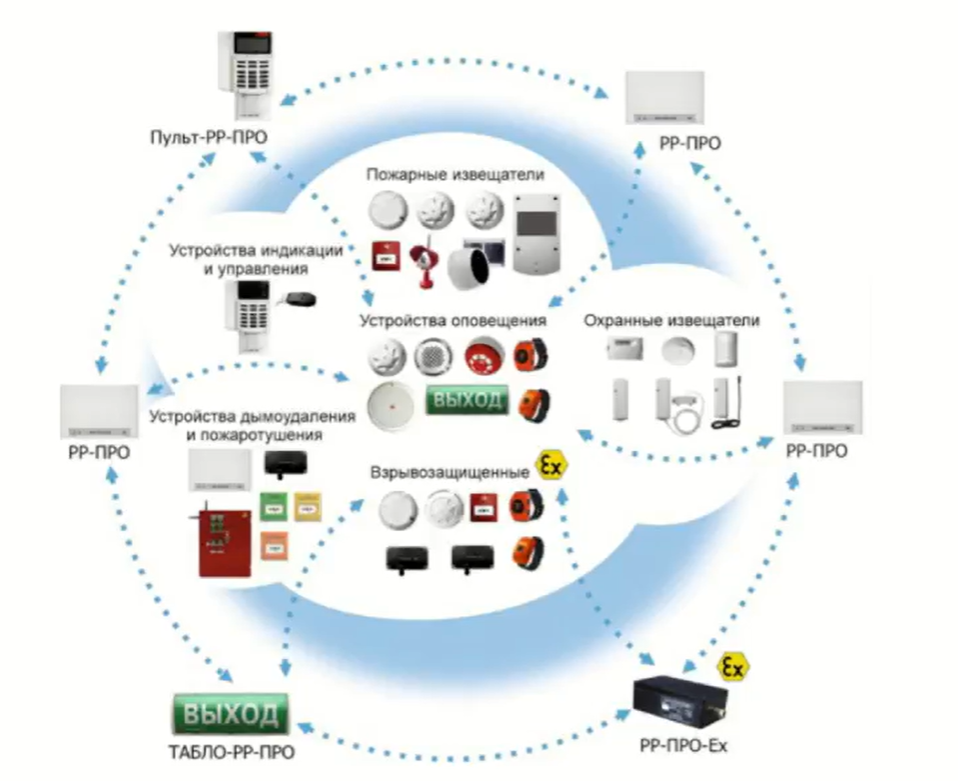
\includegraphics[width=0.8\textwidth]{image1}

Рис. 1- Беспроводная система пожарной сигнализации и автоматики,
включающая в себя облачный сервис для технологического мониторинга
{[}7{]}

В целом, умные системы детектирования пожаров имеют огромный потенциал
для обеспечения безопасности в умных городах. Однако, важно учитывать,
что каждая система имеет свои преимущества и недостатки, и выбор
конкретной системы должен основываться на специфических потребностях
города и его жителей.

Существует множество различных систем автоматического подавления
пожаров, которые используются для быстрого и эффективного тушения
возгораний. Некоторые из них включают (Рис. 2):

\begin{itemize}
\item
  Системы автоматического пожаротушения на основе газов. Эти системы
  используют различные газы, такие как аргон, диоксид углерода, азот или
  инертные газы, для тушения пожара. Газы подаются в помещение через
  сеть трубопроводов и распыляются по всей площади. Газы поглощают
  тепло, замедляют химические реакции и удаляют кислород, что приводит к
  ликвидации пожара.
\item
  Системы автоматического пожаротушения на основе жидкостей. Эти системы
  используют жидкие вещества, такие как вода, пены или специальные
  жидкости, для тушения пожара. Жидкости подаются в помещение через сеть
  трубопроводов и распыляются на поверхности горящих материалов.
  Жидкости охлаждают горящие поверхности, удаляют тепло и предотвращают
  распространение пламени.
\item
  Системы автоматического пожаротушения на основе порошков. Эти системы
  используют порошки, такие как сульфат алюминия или бикарбонат натрия,
  для тушения пожара. Порошки подаются в помещение через сеть
  трубопроводов и распыляются на поверхности горящих материалов. Порошки
  задерживают кислород, замедляют химические реакции и удаляют тепло,
  что приводит к ликвидированию пожара.
\item
  Системы автоматического пожаротушения на основе пены. Эти системы
  используют пену, которая создается путем смешивания воды и
  специального раствора, для тушения пожара. Пена подаются в помещение
  через сеть трубопроводов и распыляются на поверхности горящих
  материалов. Пена уменьшает количество кислорода, снижает температуру и
  удаляет тепло, что приводит к тушению пожара.
\end{itemize}

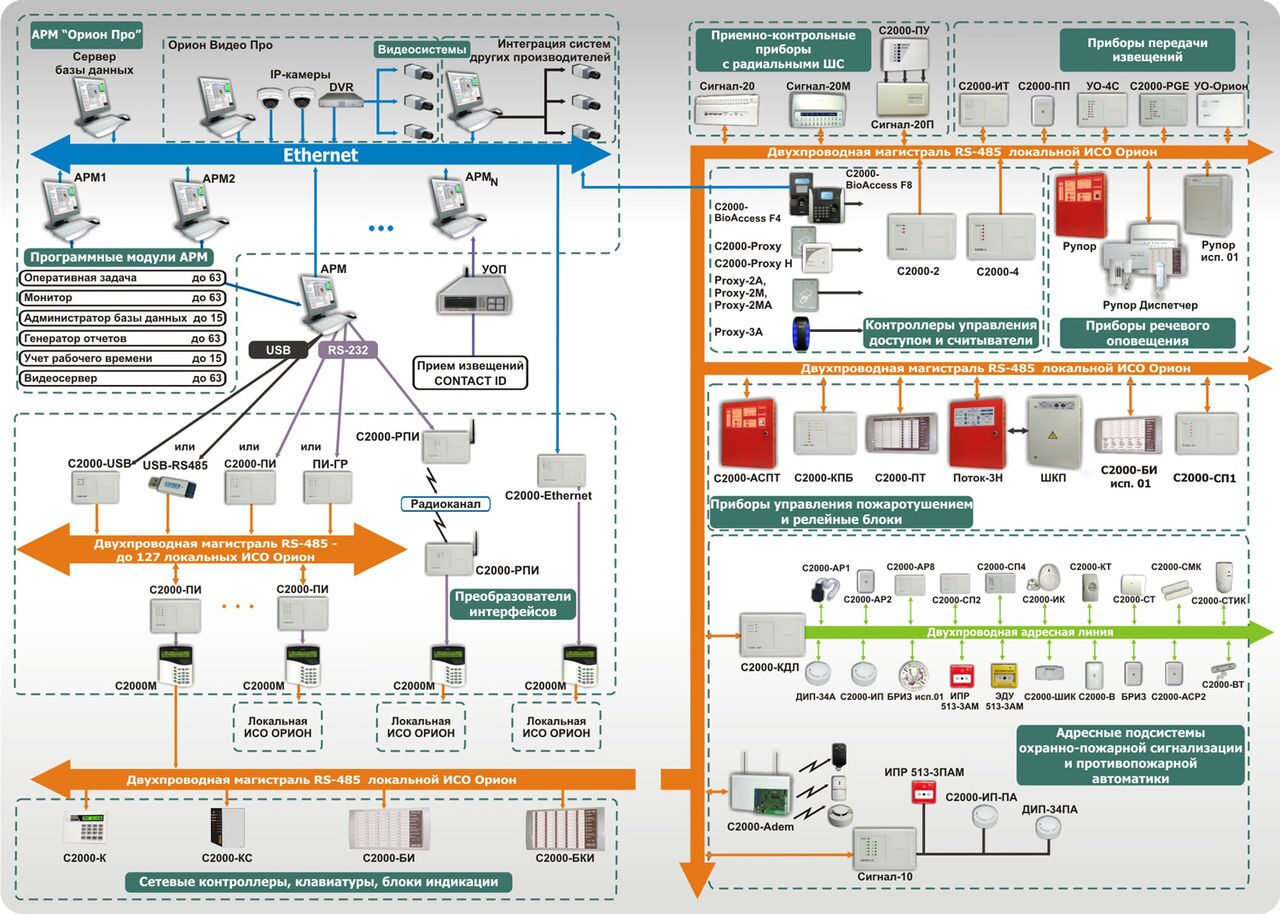
\includegraphics[width=0.8\textwidth]{image2}

Рис. 2- Пример построения пожарной сигнализации на основе системы BOLID,
которая включает три автоматические установки пожаротушения (порошковое,
газовое, водяное)

Каждая система автоматического подавления пожаров имеет свои
преимущества и недостатки. Ниже приведены некоторые из них:

Система автоматического пожаротушения водой:

Преимущества:

\begin{enumerate}
\def\labelenumi{\arabic{enumi}.}
\item
  Это наиболее распространенная и экономически выгодная система тушения
  пожара.
\item
  Вода доступна повсюду и является относительно дешевым ресурсом.
\item
  Она недорога в установке и обслуживании.
\item
  Система довольно проста в использовании.
\end{enumerate}

Недостатки:

\begin{enumerate}
\def\labelenumi{\arabic{enumi}.}
\item
  Вода может нанести вред имуществу, которое находится в зоне пожара.
\item
  Она неэффективна при тушении пожаров, связанных с электрооборудованием
  и маслом.
\item
  При наличии чрезмерного количества воды может возникнуть опасность
  затопления здания.
\end{enumerate}

Система автоматического пожаротушения газом:

Преимущества:

\begin{enumerate}
\def\labelenumi{\arabic{enumi}.}
\item
  Газы, такие как углекислый газ, галогенные газы и аргон, не повреждают
  имущество при тушении пожара.
\item
  Газы не оставляют следов и не оказывают негативного влияния на
  окружающую среду.
\item
  Система автоматического пожаротушения газом может быть легко
  интегрирована в существующую систему пожарной безопасности.
\end{enumerate}

Недостатки:

\begin{enumerate}
\def\labelenumi{\arabic{enumi}.}
\item
  Газы могут быть опасными для здоровья людей и животных.
\item
  Система автоматического пожаротушения газом может быть дорогой в
  установке и обслуживании.
\end{enumerate}

Система автоматического пожаротушения пеной:

Преимущества:

\begin{enumerate}
\def\labelenumi{\arabic{enumi}.}
\item
  Пена не повреждает имущество при тушении пожара.
\item
  Система автоматического пожаротушения пеной работает очень быстро и
  эффективно.
\item
  Пена обладает дополнительными свойствами охлаждения, которые могут
  помочь предотвратить повторное возгорание.
\end{enumerate}

Недостатки:

\begin{enumerate}
\def\labelenumi{\arabic{enumi}.}
\item
  Пена может вызывать коррозию электрооборудования.
\item
  Система автоматического пожаротушения пеной может быть дорогой в
  установке и обслуживании.
\end{enumerate}

Система автоматического пожаротушения порошком:

Преимущества:

\begin{enumerate}
\def\labelenumi{\arabic{enumi}.}
\item
  Порошок быстро тушит пожар, потому что быстро затушивает пламя и
  снижает температуру.
\item
  Порошковые системы довольно надежны и могут использоваться для тушения
  различных типов пожаров, включая горючие жидкости, газы и твердые
  вещества.
\item
  Порошковые системы относительно просты в использовании и обслуживании.
\end{enumerate}

Недостатки:

\begin{enumerate}
\def\labelenumi{\arabic{enumi}.}
\item
  Порошок может оставлять остатки на поверхностях, что может быть
  проблемой для некоторых промышленных процессов.
\item
  Порошковые системы не подходят для использования в областях с высокой
  влажностью, так как вода может склеивать порошок и делать его менее
  эффективным.
\item
  Порошок может быть вреден для животных и людей, поэтому следует быть
  осторожными при использовании в жилых зонах.
\end{enumerate}

Система автоматического пожаротушения углекислым газом:

Преимущества:

\begin{enumerate}
\def\labelenumi{\arabic{enumi}.}
\item
  Углекислый газ быстро тушит пожары и не оставляет остатков.
\item
  Углекислый газ не повреждает электронное оборудование и другие
  чувствительные предметы.
\item
  Системы тушения углекислым газом могут использоваться в небольших и
  крупных помещениях.
\end{enumerate}

Недостатки:

\begin{enumerate}
\def\labelenumi{\arabic{enumi}.}
\item
  Углекислый газ может быть опасен для людей, поэтому следует быть
  осторожными при использовании в жилых зонах.
\item
  Углекислый газ может быть дорогим в производстве, что может повлиять
  на стоимость системы пожаротушения.
\item
  Системы тушения углекислым газом могут потребовать дополнительных
  работ по установке и обслуживанию, что может повлиять на стоимость и
  сложность системы.
\end{enumerate}

Некоторые примеры реализации систем автоматического подавления пожаров в
умных городах:

\begin{itemize}
\item
  Шанхай, Китай: В рамках проекта по созданию умного города в Шанхае
  были установлены системы автоматического пожаротушения в некоторых
  зданиях и объектах города, включая жилые дома, торговые центры и
  склады. Системы используют различные методы тушения пожара, включая
  использование воды, газов и порошка.
\item
  Сеул, Южная Корея: В Сеуле были установлены системы автоматического
  пожаротушения в метрополитене города. Системы используют воду для
  тушения пожаров и были разработаны с учетом особенностей
  метрополитена, включая наличие высоковольтных линий и систем
  вентиляции.
\item
  Дубай, ОАЭ: В Дубае была установлена система автоматического
  пожаротушения в самом высоком здании в мире - небоскребе Burj Khalifa.
  Система использует воду для тушения пожаров и была разработана с
  учетом особенностей здания, включая его высоту и сложную архитектуру.
  Городская команда пожарных внедрила систему Fireye, которая использует
  искусственный интеллект для обнаружения возгораний и автоматического
  оповещения пожарных. Система включает в себя более 16 000 датчиков и
  позволяет реагировать на пожары мгновенно.
\item
  Город Копенгаген в Дании: в Копенгагене внедрена система пожарной
  безопасности, которая использует данные датчиков качества воздуха для
  обнаружения изменений в концентрации угарного газа и оповещения о
  пожарах.
\item
  Город Торонто в Канаде: в Торонто внедрена система пожарной
  безопасности, которая использует умные датчики, установленные на
  каждом этаже здания, для обнаружения пожаров. Датчики синхронизированы
  с центральной системой управления, которая автоматически оповещает
  пожарных и предоставляет информацию о месте возгорания.
\item
  Город Сеул в Южной Корее: в Сеуле установлены умные датчики дыма,
  которые используются для обнаружения пожаров в многоэтажных зданиях.
  Датчики сигнализируют о пожаре, а затем система автоматического
  пожаротушения, установленная на каждом этаже, начинает работу.
\item
  Барселона, Испания: В Барселоне была установлена система
  автоматического пожаротушения в здании местного музея. Система
  использует газ для тушения пожаров и была разработана с учетом
  особенностей здания, включая его историческую ценность и наличие
  хрупких экспонатов.
\end{itemize}

Умные системы управления пожаром используют сенсоры и другие технологии,
чтобы обнаруживать пожары и принимать соответствующие меры для их
тушения. Они могут включать в себя следующие компоненты (Рис. 3):

\begin{itemize}
\item
  Системы управления пожаротушением: эти системы используют различные
  технологии, такие как датчики дыма и тепла, чтобы обнаруживать пожары
  и автоматически активировать системы пожаротушения, такие как системы
  дренажных шлангов и автоматические установки пожаротушения.
\item
  Системы управления дверьми: эти системы используются для контроля
  доступа и предотвращения распространения огня через двери. Они могут
  быть программируемыми для автоматического закрытия и блокировки
  дверей, если возникает пожар.
\item
  Системы управления эвакуацией: эти системы предназначены для быстрой и
  эффективной эвакуации людей из здания в случае пожара. Они могут
  включать в себя автоматические оповещения и инструкции для эвакуации,
  системы связи и навигации, а также интегрированные системы контроля
  доступа для предотвращения паники и хаоса.
\item
  Системы мониторинга окружающей среды: эти системы используют сенсоры
  для наблюдения за уровнем кислорода, угарного газа и других вредных
  веществ в окружающей среде. Они также могут контролировать температуру
  и влажность, чтобы определить риски возгорания.
\end{itemize}

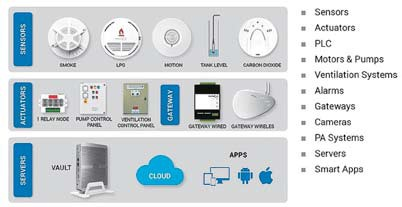
\includegraphics[width=0.8\textwidth]{image3}

Рис. 3 - Элементы системы пожарной безопасности на основе IoT

Примеры умных систем управления пожаром включают в себя систему
«СМАРТ-ПОЖАР» в Москве, которая включает в себя датчики дыма, тепла и
газа, а также систему оповещения и навигации для эвакуации людей.

Еще один пример - система управления пожаром в торговом центре «Cityon
Xi\textquotesingle an» в Китае, которая включает в себя системы
мониторинга окружающей среды, автоматические установки пожаротушения и
систему управления дверьми для предотвращения распространения огня.

Ниже приведены преимущества и недостатки нескольких типов умных систем
управления пожаром:

Системы управления пожаром на основе облака данных.

Преимущества:

\begin{enumerate}
\def\labelenumi{\arabic{enumi}.}
\item
  Можно использовать в любом масштабе: от небольшого здания до крупного
  города.
\item
  Может быстро определить местоположение пожара и отправить сообщения на
  мобильные устройства или в офисы службы пожарной безопасности.
\item
  Система может автоматически предоставлять рекомендации по эвакуации и
  другие инструкции по безопасности.
\end{enumerate}

Недостатки:

\begin{enumerate}
\def\labelenumi{\arabic{enumi}.}
\item
  Требуется надежное подключение к Интернету для полной
  функциональности.
\item
  Неэффективна в случаях, когда необходимо быстрое действие и устранение
  проблемы немедленно.
\item
  Могут возникать проблемы с конфиденциальностью данных в случае
  нарушения системы.
\end{enumerate}

Системы управления пожаром на основе искусственного интеллекта.

Преимущества:

\begin{enumerate}
\def\labelenumi{\arabic{enumi}.}
\item
  Системы на основе искусственного интеллекта могут эффективно
  анализировать данные для определения наличия пожара и его
  местоположения.
\item
  Могут предсказывать вероятность возникновения пожаров на основе данных
  о климате и других факторах.
\item
  Могут автоматически управлять системами тушения пожара и производить
  эвакуацию.
\end{enumerate}

Недостатки:

\begin{enumerate}
\def\labelenumi{\arabic{enumi}.}
\item
  Требуется большой объем данных для корректной работы системы.
\item
  Могут возникать проблемы с точностью анализа, особенно при сильном
  дыме или других факторах, которые затрудняют обнаружение пожара.
\item
  Высокая стоимость.
\end{enumerate}

Системы управления пожаром на основе IoT-технологий {[}8, 9{]}.

Преимущества:

\begin{enumerate}
\def\labelenumi{\arabic{enumi}.}
\item
  Большое количество устройств IoT, таких как датчики температуры, дыма
  и движения, могут быть интегрированы в систему, что позволяет получать
  много информации о возможных угрозах пожара.
\item
  Использование аналитических данных позволяет определять оптимальную
  стратегию тушения пожара и уменьшает время реакции на пожар.
\item
  Информация о пожаре может быть передана автоматически в системы
  управления, вызова пожарных служб, а также на мобильные устройства
  пользователя.
\item
  Системы управления пожаром на основе IoT-технологий могут
  использоваться для управления несколькими объектами одновременно, что
  может существенно повысить эффективность.
\item
  Технология IoT может использоваться для прогнозирования возможных
  рисков пожара, что помогает предотвращать возникновение пожаров в
  будущем.
\end{enumerate}

Недостатки:

\begin{enumerate}
\def\labelenumi{\arabic{enumi}.}
\item
  Риск возникновения ошибок в системе IoT. Если один из датчиков или
  устройств не будет работать должным образом, это может привести к
  неверной оценке угрозы пожара и неправильной реакции на пожар.
\item
  Высокая стоимость оборудования и инфраструктуры, необходимых для
  установки системы управления пожаром на основе IoT-технологий.
\item
  Требуется надежное соединение с интернетом и устойчивая работа сети
  для обмена данными между устройствами.
\item
  Некоторые системы могут быть сложны в установке и настройке, требуя
  профессиональных навыков.
\item
  Защита конфиденциальности и безопасности данных, передаваемых между
  устройствами IoT, может стать проблемой, особенно в случае хакерских
  атак или несанкционированного доступа.
\end{enumerate}

Несколько примеров реализации систем управления пожаром на основе
IoT-технологий в умных городах (Рис. 4):

\begin{itemize}
\item
  Санта-Клара, Калифорния, США - В 2019 году город Санта-Клара в
  Калифорнии внедрил систему управления пожаром на основе
  IoT-технологий. Система включает в себя датчики дыма, температуры,
  влажности, CO2 и движения, которые мониторят изменения в окружающей
  среде и передают данные в облако, где они анализируются и используются
  для принятия решений о тушении пожара. Система также имеет
  автоматический вызов пожарных служб, если датчики обнаружат признаки
  пожара.
\item
  Сингапур - В Сингапуре была разработана система управления пожаром на
  основе IoT-технологий, которая используется в высотных зданиях.
  Система включает в себя датчики температуры, давления, дыма и газа,
  которые мониторят изменения в окружающей среде и передают данные на
  сервер, где они анализируются. Если датчики обнаружат признаки пожара,
  система автоматически отправляет сообщение на пульт управления и
  вызывает пожарных.
\item
  Гамбург, Германия - Город Гамбург в Германии внедрил систему
  управления пожаром на основе IoT-технологий, которая используется в
  туннелях и метро. Система включает в себя датчики дыма, температуры и
  CO2, которые мониторят изменения в окружающей среде и передают данные
  на сервер, где они анализируются. Если датчики обнаружат признаки
  пожара, система автоматически отправляет сообщение на пульт управления
  и вызывает пожарных.
\item
  Город Копенгаген в Дании установил систему, которая объединяет датчики
  дыма, системы оповещения и системы дистанционного управления в единую
  систему управления пожарной безопасностью. Система собирает данные о
  дыме и температуре и передает их на центральный сервер. Если
  происходит пожар, система автоматически оповещает пожарную службу, а
  также отправляет информацию о местоположении пожара и его
  характеристиках.
\item
  В Дубае установлены умные системы управления пожарной безопасностью в
  высотных зданиях. Эти системы используют датчики дыма и температуры,
  которые мониторят пожарную опасность. Когда система обнаруживает
  пожар, она автоматически срабатывает, закрывая вентиляционные
  отверстия, чтобы предотвратить распространение огня, и уведомляет
  службу пожарной безопасности.
\item
  Город Барселона в Испании использует умную систему управления пожарной
  безопасностью на своих улицах. Система включает датчики дыма и
  температуры, которые мониторят общественные пространства, и систему
  оповещения, которая автоматически оповещает службу пожарной
  безопасности в случае возникновения пожара. Система также включает
  автоматические системы пожаротушения, которые могут быстро подавить
  пожар, прежде чем он начнет распространяться.
\end{itemize}

Это лишь некоторые примеры систем управления пожаром на основе
IoT-технологий, реализованных в различных умных городах по всему миру.

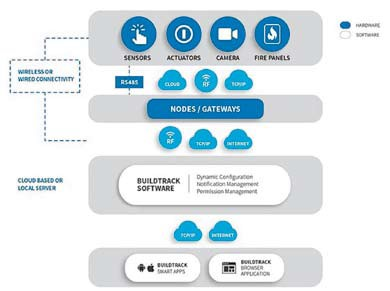
\includegraphics[width=0.8\textwidth]{image4}

Рис. 4 - Стандартная архитектура системы пожарной безопасности на основе
IoT

Системы оповещения и эвакуации граждан являются важной частью общей
системы пожарной безопасности. Они предназначены для предупреждения
людей о возможной опасности и организации эвакуации в случае пожара.
Существуют различные типы систем оповещения и эвакуации граждан, которые
могут быть использованы в зависимости от конкретной ситуации.

Одним из наиболее распространенных типов систем оповещения является
система громкоговорителей. Она включает в себя установку
громкоговорителей в зданиях и на улицах города, которые могут
воспроизводить звуковые сигналы для предупреждения людей о возможной
опасности. Некоторые системы громкоговорителей также могут
использоваться для оповещения людей о том, что они могут покинуть здание
в случае пожара.

Еще один тип системы оповещения -- это система SMS-уведомлений. Она
используется для отправки SMS-сообщений на мобильные телефоны людей,
которые зарегистрировали свои номера в системе. Такие системы могут быть
особенно полезны в крупных городах, где многие люди постоянно находятся
в движении.

Существуют также системы оповещения и эвакуации на основе световых
сигналов. Они могут использоваться в сочетании с системами
громкоговорителей или отдельно. Например, система оповещения на основе
световых сигналов может быть установлена в здании и использоваться для
предупреждения людей о пожаре, если в помещении слишком шумно для того,
чтобы использовать громкоговорители.

Кроме того, существуют также автоматические системы оповещения, которые
могут быть интегрированы с другими умными системами пожарной
безопасности. Например, система детектирования пожара на основе дыма
может быть интегрирована с системой оповещения для автоматического
предупреждения людей в здании о возможной опасности.

Все системы оповещения и эвакуации граждан имеют свои преимущества и
недостатки, которые могут зависеть от конкретных обстоятельств.

Далее приведены преимущества и недостатки некоторых распространенных
систем оповещения и эвакуации граждан:

Звуковая система оповещения и эвакуации. Это самый распространенный и
простой вид системы, который использует звуковой сигнал для оповещения и
направления людей на выход из здания.

Преимущества:

\begin{enumerate}
\def\labelenumi{\arabic{enumi}.}
\item
  Простота установки и использования;
\item
  Низкая стоимость.
\end{enumerate}

Недостатки:

\begin{enumerate}
\def\labelenumi{\arabic{enumi}.}
\item
  Неэффективность для людей со слабым слухом;
\item
  Ограниченность в передаче информации о характере и местоположении
  пожара.
\end{enumerate}

Система оповещения и эвакуации на основе световых сигналов. Эта система
использует световые сигналы, такие как мигающие огни, для оповещения и
направления людей к выходу из здания.

Преимущества:

\begin{enumerate}
\def\labelenumi{\arabic{enumi}.}
\item
  Эффективность для людей со слабым слухом;
\item
  Хорошая видимость в темноте.
\end{enumerate}

Недостатки:

\begin{enumerate}
\def\labelenumi{\arabic{enumi}.}
\item
  Ограниченность в передаче информации о характере и местоположении
  пожара;
\item
  Высокая стоимость.
\end{enumerate}

Система оповещения и эвакуации на основе текстовых сообщений. Эта
система использует текстовые сообщения, передаваемые через мобильные
устройства или другие коммуникационные каналы, для оповещения и
направления людей к выходу из здания.

Преимущества:

\begin{enumerate}
\def\labelenumi{\arabic{enumi}.}
\item
  Может обеспечить более точную информацию о характере и местоположении
  пожара;
\item
  Хорошая эффективность для людей со слабым зрением или слухом.
\end{enumerate}

Недостатки:

\begin{enumerate}
\def\labelenumi{\arabic{enumi}.}
\item
  Требуется наличие мобильных устройств или других коммуникационных
  средств;
\item
  Неэффективность, если люди не могут или не хотят получать текстовые
  сообщения.
\end{enumerate}

Система оповещения и эвакуации на основе виртуальной реальности является
инновационным подходом к созданию системы безопасности. Она использует
технологию виртуальной реальности, чтобы обучать людей, как действовать
в случае пожара или другой аварии, а также для эвакуации.

Преимущества:

\begin{enumerate}
\def\labelenumi{\arabic{enumi}.}
\item
  Увеличивает эффективность обучения и подготовки к чрезвычайным
  ситуациям, поскольку обучение проводится в условиях виртуальной
  реальности, которая более реалистична и захватывающа.
\item
  Увеличивает эффективность эвакуации, поскольку люди могут быть более
  знакомы с территорией и знать, куда следует направляться.
\item
  Уменьшает количество жертв в чрезвычайных ситуациях, поскольку люди
  будут лучше подготовлены и обучены действовать в таких ситуациях.
\end{enumerate}

Недостатки:

\begin{enumerate}
\def\labelenumi{\arabic{enumi}.}
\item
  Системы на основе виртуальной реальности могут быть дорогостоящими для
  создания и установки.
\item
  Система требует обновлений и технического обслуживания, чтобы
  гарантировать ее надежность и эффективность.
\item
  Некоторые люди могут испытывать дискомфорт или неудобства при
  использовании виртуальной реальности, что может отвлечь их от обучения
  или эвакуации.
\end{enumerate}

Системы оповещения и эвакуации на основе виртуальной реальности являются
новым направлением в развитии умных городов, поэтому пока что не
существует множества примеров реализации таких систем в реальных
городах.

Одним из примеров реализации подобной системы является проект,
воплощенный в жизнь компанией Luminous Group. Они разработали
виртуальную реальность, которая позволяет людям испытать пожарную
опасность, не находясь на самом объекте. Система состоит из нескольких
виртуальных тренажеров, которые имитируют ситуации пожаров различной
сложности. Посетитель может научиться пользоваться огнетушителями и
другими средствами пожаротушения, а также понять, как правильно и быстро
эвакуироваться из здания.

\begin{itemize}
\item
  Еще одним примером является проект, реализованный в городе Сингапур.
  Здесь была создана система AR-очков (очки дополненной реальности),
  которая позволяет людям быстро и безопасно покинуть здание в случае
  пожара. Система сканирует помещение и отображает на очках наиболее
  безопасный путь для эвакуации.
\item
  В России проекты по созданию систем оповещения и эвакуации на основе
  виртуальной реальности пока что не широко распространены, но многие
  компании работают в этом направлении, в том числе НИИ "Криста".
\end{itemize}

Система оповещения и эвакуации на основе световых сигналов является
одной из самых распространенных и простых систем в умных городах. Она
использует специальные световые сигналы, которые сигнализируют о
необходимости эвакуации или предупреждают об опасности. Примеры
реализации этой системы можно найти по всему миру.

\begin{itemize}
\item
  Например, в Японии система оповещения и эвакуации на основе световых
  сигналов используется во многих городах, включая Токио. Световые
  сигналы размещены во многих местах, в том числе на зданиях, мостах и
  автомобильных дорогах. Они могут быть использованы для предупреждения
  о землетрясениях, цунами и других природных катастрофах.
\item
  В США система оповещения и эвакуации на основе световых сигналов
  используется для предупреждения о торнадо. В некоторых городах
  установлены специальные световые сигналы, которые могут предупредить
  жителей о торнадо и указать направление, в котором необходимо
  двигаться для эвакуации.
\item
  В России система оповещения и эвакуации на основе световых сигналов
  также широко используется в умных городах. Например, в Москве и
  Санкт-Петербурге световые сигналы установлены на зданиях, мостах и
  других объектах, и используются для оповещения жителей о пожарах,
  авариях и других чрезвычайных ситуациях.
\end{itemize}

Однако, недостатком этой системы является то, что она может быть
ограничена в использовании в темное время суток или в условиях, когда
видимость снижена из-за дыма или тумана. Кроме того, световые сигналы
могут быть не заметны для людей с ограниченными возможностями зрения
(Рис. 5).

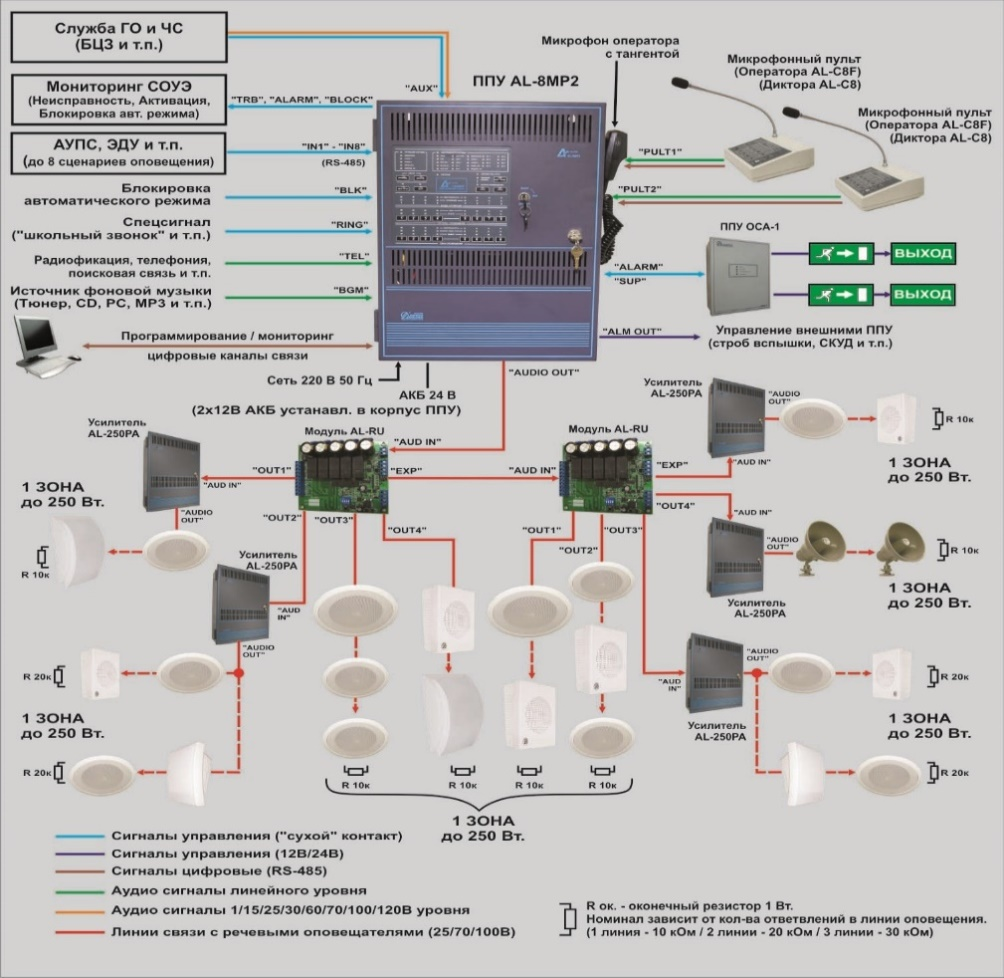
\includegraphics[width=0.8\textwidth]{image5}

Рис. 5 - Система речевого оповещения о пожаре серии Альфа

Сравнение различных систем пожарной безопасности зависит от многих
факторов, включая тип здания, его назначение, размер и наличие
персонала. Ниже приведены общие характеристики и сравнение нескольких
типов систем пожарной безопасности.

Системы автоматического пожаротушения:

Преимущества: эффективность, автоматическое действие, надежность.

Недостатки: возможно повреждение имущества, высокая стоимость установки
и технического обслуживания.

Системы оповещения и эвакуации:

Преимущества: быстрое оповещение, возможность эвакуации, надежность.

Недостатки: требуют обучения и знания о процедурах эвакуации, могут
вызывать панику в людях, не способных на нормальное восприятие звуков.

Системы детектирования пожаров:

Преимущества: быстрое обнаружение пожара, возможность автоматической
активации других систем безопасности.

Недостатки: ложные срабатывания, высокая стоимость установки и
технического обслуживания.

Системы пассивной защиты от пожара:

Преимущества: надежность, эффективность, низкая стоимость.

Недостатки: не действуют на пожарном стадии, не способны обнаруживать
пожар.

Системы управления пожаром на основе IoT-технологий:

Преимущества: точность, быстрое обнаружение и управление пожаром,
удаленное управление, снижение вероятности ложных срабатываний.

Недостатки: высокая стоимость, сложность в установке и техническом
обслуживании.

Применимость разных систем пожарной безопасности может зависеть от
конкретных городских условий, таких как климат, наличие промышленных
зон, плотность населения и т.д. Например, в городах, где климат холодный
и снежный, система автоматического тушения пожаров водой может быть
менее эффективной из-за возможности замерзания воды и образования льда,
что затруднит доступ к возгоранию и усложнит работу пожарных.

С другой стороны, в городах с промышленными зонами, где может быть
большое количество горючих материалов и легко воспламеняемых веществ,
могут быть эффективны системы автоматического тушения пожаров, которые
используют специализированные химические вещества, такие как инертные
газы или порошок.

Также важным фактором может быть плотность населения и густота
застройки. В городах с большой плотностью населения и высокой застройкой
может быть трудно провести эвакуацию людей в случае пожара, поэтому
могут быть эффективны системы оповещения и эвакуации, которые используют
визуальные и звуковые сигналы, чтобы привлечь внимание граждан и
направить их на безопасный выход.

Таким образом, выбор системы пожарной безопасности должен основываться
на конкретных условиях города и требованиях к безопасности, а также на
эффективности, надежности и стоимости реализации и эксплуатации системы.

Умные технологии имеют огромный потенциал для улучшения систем пожарной
безопасности в умных городах. Многие инновации уже внедрены и успешно
работают, позволяя ускорить процессы обнаружения и тушения пожаров,
оповещения и эвакуации населения, а также минимизации ущерба от пожара
(Рис. 6).

Системы оповещения и эвакуации на основе IoT-технологий и виртуальной
реальности позволяют быстро обнаружить пожар и организовать эвакуацию,
даже если люди находятся внутри зданий, где не ощущают запах дыма или не
видят огонь. Автоматические системы пожаротушения на основе газа, пены,
порошка и воды позволяют быстро потушить пожар и предотвратить
распространение огня.

Системы мониторинга и детектирования пожаров, основанные на датчиках и
анализе больших данных, позволяют быстро обнаружить начальные стадии
пожара и принять меры для его тушения. Автоматические системы управления
пожаром на основе IoT-технологий позволяют быстро реагировать на пожар и
координировать действия пожарных бригад {[}10, 11{]}.

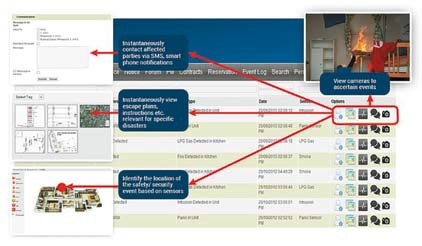
\includegraphics[width=0.8\textwidth]{image6}

Рис. 6 - Пример централизованной системы контроля, позволяющей выявлять
чрезвычайные ситуации в пределах обширной территории

Каждая из систем имеет свои преимущества и недостатки, и выбор
конкретной системы должен основываться на характеристиках конкретного
города и его потребностях. Однако все они могут быть успешно
интегрированы в общую систему пожарной безопасности, что позволит
значительно повысить ее эффективность.

\textbf{Выводы.} Умные системы пожарной безопасности имеют большой
потенциал для развития в будущем. С появлением новых технологий и
развитием искусственного интеллекта, умные системы пожарной безопасности
будут становиться все более эффективными и точными в предотвращении и
тушении пожаров. Одной из перспективных технологий является
использование беспилотных авиационных систем для наблюдения и тушения
пожаров, особенно там, где доступ человека затруднен или опасен. Также в
будущем умные системы пожарной безопасности могут быть установлены во
всех зданиях и сооружениях, и интегрированы с другими умными системами
города, такими как системы мониторинга качества воздуха, системы
управления транспортом и энергетические сети. Другой перспективной
технологией является использование блокчейн-технологии для создания
безопасных и надежных систем пожарной безопасности. Блокчейн может
обеспечить децентрализованное хранение данных о системах пожарной
безопасности и связанных с ними рисках, что может помочь в
предотвращении пожаров и быстрой реакции на них.

В целом, умные технологии имеют огромный потенциал для улучшения систем
пожарной безопасности в умных городах, что может привести к снижению
рисков и сохранению жизней.

\emph{Работа выполнена за счет средств грантового финансирования научных
исследований на 2023-2025 годы по проекту ИРН АР19678157.}

\textbf{Литература}

1. Ву Т.З. Анализ систем автоматизированного управления умным домом //
Молодой ученый, 2011. -- №4. Т.1. -- С. 28-29. (in Eng).

2. А.Ф. Котюк. Датчики в современных измерениях. -- М.: «Радио и связь»,
2006. -- 96 с. (in Russ).

3. Дж. Фрайден. Современные датчики. -- М.: «Техносфера», 2005. -- 592
с. (in Russ).

4. Е.А. Тесля. «Умный дом» своими руками. Строим интеллектуальную
цифровую систему в своей квартире / Тесля Е.А. -- СПб., 2008. -- 224 с.
(in Russ).

5. Intelligent Buildings: Design, Management \& Operation / edited by
Derek Clements-Croome. -- London: Thomas Telford Publishing, 2004. --
408 p. (in Eng).

6. Г.З. Зиятбекова, А.Т. Мазакова, А.Д. Бургегулов, Е.Б. Муратов.
Разработка энергосберегающей системы «Умный офис» и его принципы работы
// Вестник КазУТБ. -- Нур-Султан, 2022. -- № 1(14). -- С. 13-18. (in
Russ).

7. Ч. Платт. Электроника: логические микросхемы, усилители и датчики для
начинающих. -- СПб.: БХВ-Петербург, 2015. -- 448 с. (in Eng).

8. Т. Рашид. Создаем нейронную сеть. -- СПб.: ООО «Альфа-книга», 2018.
-- 272 с. (in Russ).

9. К.Е. Климентьев. Системы реального времени. -- Самара: Самар.гос.
аэрокосм. ун-т, 2008. -- 45 с. (in Russ).

10. Р. Каллан. Нейронные сети. Краткий справочник -- М.: ООО «И.Д.
Вильямс», 2017. -- 288 с. (in Russ).

11. С.В. Аксенов, В.Б. Новосельцев. Организация и использование
нейронных сетей (методы и технологии). -- Томск: Изд-во НТЛ, 2006. --
128 с. (in Russ).

\textbf{References}

1. Wu T.Z. Analysis of automated control systems for smart house //
Young Scientist, 2011. -- No. 4. -- VOL. 1. -- Pр. 28-29. (in Eng)

2. A.F. Kotyuk. Sensors in Modern Measurements. -- M.: Radio and
Communications, 2006. -- 96 p. (in Russ)

3. J. Fryden. Modern Sensors. -- M.: Technosphere, 2005. -- 592 p. (in
Russ)

4. E.A. Tesla. "Smart House with my own hands. Building an intelligent
digital system in your apartment / Teslya E.A. -- SPb., 2008. -- 224 p.
(in Russ)

5. Intelligent Buildings: Design, Management \& Operation / edited by
Derek Clements-Croome. -- London: Thomas Telford Publishing, 2004. --
408 p. (in Eng)

6. G.Z. Ziyatbekova, A.T. Mazakova, A.D. Burgegulov, E.B. Muratov.
Development of energy-saving system "Smart Office" and its operating
principles // Bulletin of KazUTB. -- Nur-Sultan, 2022. -- No. 1(14). --
Pp. 13-18. (in Russ)

7. Ch. Platt. Electronics: Logic Circuits, Amplifiers and Sensors for
Beginners. -- SPb: BHV-Peterburg, 2015. -- 448 p. (in Eng)

8. Т. Rashid. Creating a neural network. -- St. Petersburg: OOO
"Alpha-book", 2018. -- 272 p. (in Russ)

9. K.E. Klimentiev. Real-time systems. -- Samara: Samara State Aerospace
University, 2008. -- 45 p. (in Russ)

10. Р. Callan. Neural networks. A Quick Reference Guide. -- M.: I.D.
Williams LLC, 2017. -- 288 p. (in Russ)

11. S.V. Aksenov, V.B. Novoseltsev. Organization and use of neural
networks (methods and technologies). -- Tomsk: NTL Publisher, 2006. --
128 p. (in Russ)

\emph{\textbf{Сведения об авторах}}

Бургегулов А. Д. -- докторант КазНУ имени аль-Фараби, Алматы, Казахстан,
\href{mailto:dizel_kz@bk.ru}{\nolinkurl{dizel\_kz@bk.ru}}

Мазаков Т.Ж. -- доктор физико-математических наук, главный научный
сотрудник Института Информационных и вычислительных технологий КН МНВО
РК, профессор НАО Казахского национального университета имени
аль-Фараби, Алматы, Казахстан,
\href{mailto:tmazakov@mail.ru}{\nolinkurl{tmazakov@mail.ru}}

Зиятбекова Г.З. -- PhD, и.о. доцента НАО Казахского национального
университета имени аль-Фараби; старший научный сотрудник Института
Информационных и вычислительных технологий КН МНВО РК, Алматы,
Казахстан,
\href{mailto:ziyatbekova@mail.ru}{\nolinkurl{ziyatbekova@mail.ru}}

Саметова А.А. -- докторант КазНУ имени аль-Фараби, Алматы, Казахстан,
sametova\_aygerim\href{mailto:amirkhanov.b@gmail.com}{@mail.}ru

Джолдасова Б.У. -- магистрант КазНУ имени аль-Фараби, Алматы, Казахстан,
bagilaurel@gmail.com

\emph{\textbf{Information about authors}}

Burgegulov A. D. -- doctoral student at Al-Farabi Kazakh National
University, Almaty, Kazakhstan, dizel\_kz@bk.ru

Mazakov T. Zh. -- NAO Al-Farabi Kazakh National University, doctor of
physical and mathematical sciences, professor, Almaty, Kazakhstan, Chief
Researcher at the RSE Institute of Information and Computational
Technologies of the National Academy of Sciences of the Republic of
Kazakhstan, Almaty, Kazakhstan,
\href{mailto:tmazakov@mail.ru}{\nolinkurl{tmazakov@mail.ru}}

Ziyatbekova G. Z. -- PhD, Acting Associate Professor NAO Al-Farabi
Kazakh National University; Senior Researcher at the RSE Institute of
Information and Computational Technologies of the National Academy of
Sciences of the Republic of Kazakhstan, Almaty, Kazakhstan,
ziyatbekova@mail.ru

Sametova Aigerim Aidarkyzy -- doctoral student at Al-Farabi Kazakh
National University, Almaty, Kazakhstan,
sametova\_aygerim\href{mailto:amirkhanov.b@gmail.com}{@mail.}ru

Joldassova Bagila Ummetovna -- graduate student at Al-Farabi Kazakh
National University, Almaty, Kazakhstan, bagilaurel@gmail.com

\textbf{SRSTI 50.47.00:20.23.19}

\textbf{DATAMINING CAPABILITIES FOR CLUSTERING CONCRETE MIX
FORMULATIONS}

\textbf{K.M. Akishev\textsuperscript{1*},V.I. Karpov\textsuperscript{2},
L.A. Akisheva\textsuperscript{3}, A.D.Tulegulov\textsuperscript{1}}

\textsuperscript{1}Kazhach University of Technology and
Business,\textsuperscript{2}Moscow State University of Technology and
Management named after K.G. Razumovsky, \textsuperscript{3}Nazarbayev
Intellectual School

e-mail:\href{mailto:Akmail04cx@mail.ru}{\nolinkurl{Akmail04cx@mail.ru}}

The article discusses the possibilities of using DataMining technology
for clustering concrete mixtures. In practice, it is often necessary to
face tasks in which it is necessary to choose the formulations closest
in quality characteristics from a large number of formulations of
concrete mixtures. The distribution of formulations of concrete mixtures
by classes is provided on the basis of specified criteria such as
strength, as well as the composition of the ingredients of the concrete
mixture. Earlier in work {[}1{]}, clustering of concrete mix
formulations was carried out with the help of the program "Comprehensive
quality assessment and classification of multidimensional objects",
which made it possible to distribute formulations into classes with the
closest characteristics and collect the highest quality concrete mix
formulations into the appropriate classes. The result of using
DataMining technology for clustering concrete mix formulations allowed
us to create classes in which the distribution using the DBSCAN
algorithm is quite high-quality, however, there is a need for more
detailed training of this algorithm, since clustering using the program
"Integrated Quality Assessment and classification of multidimensional
objects" turned out to be more optimal.

\textbf{Keywords} : clustering, datamining, concrete mix formulations,
quality criteria

\textbf{БЕТОН ҚОСПАЛАРЫНЫҢ РЕЦЕПТЕРІН КЛАСТЕРЛЕУГЕ АРНАЛҒАН DATA MINING
МҮМКІНДІКТЕРІ}

\textbf{К.М.Акишев\textsuperscript{1*}, В.И.Карпов\textsuperscript{2},
Л.Ақышева\textsuperscript{3}, А.Д.Тулеғулов\textsuperscript{1}}

\textsuperscript{1}Қазақ технология және бизнес университеті,
\textsuperscript{2} К. Г. Разумовский атындағы Москеу мемлекеттік
технология және басқару университеті

\textsuperscript{3} Назарбаев Зияткерлік мектебі,

e-mail: \href{mailto:Akmail04cx@mail.ru}{\nolinkurl{Akmail04cx@mail.ru}}

Мақалада бетон қоспаларын кластерлеу үшін DataMining технологиясын
қолдану мүмкіндіктері қарастырылады. Іс жүзінде сіз көбінесе бетон
қоспаларының көптеген рецептерінен сапалық сипаттамалары бойынша ең
жақын рецептілерді таңдау қажет болатын міндеттерге тап болуыңыз керек.
Бетон қоспаларының рецептураларын сыныптар бойынша бөлу беріктік,
сондай-ақ бетон қоспасының ингредиенттерінің құрамы сияқты берілген
критерийлер негізінде қамтамасыз етіледі. {[}1{]} -жұмыстың басында
бетон қоспаларының рецептураларын кластерлеу "сапаны кешенді бағалау
және көпөлшемді объектілерді жіктеу" бағдарламасының көмегімен жүзеге
асырылды, бұл рецептураларды ең жақын сипаттамалары бар сыныптарға
бөлуге және бетон қоспаларының ең сапалы рецептураларын тиісті
сыныптарға жинауға мүмкіндік берді. Бетон қоспаларының формулаларын
кластерлеу үшін DataMining технологиясын қолданудың нәтижесі DBSCAN
алгоритмін қолдана отырып бөлу өте сапалы болатын сыныптар құруға
мүмкіндік берді, дегенмен бұл алгоритмді егжей-тегжейлі оқыту қажет,
өйткені "сапаны кешенді бағалау және көп өлшемді объектілерді жіктеу"
бағдарламасын қолдана отырып кластерлеу оңтайлы болды.

\textbf{Түйін сөздер}: кластерлеу, datamining, бетон қоспаларының
формулалары, сапа критерийлері.

\textbf{ВОЗМОЖНОСТИ DATAMINING ДЛЯ КЛАСТЕРИЗАЦИИ РЕЦЕПТУР БЕТОННЫХ
СМЕСЕЙ}

\textbf{К.М.Акишев\textsuperscript{1*}, В.И.Карпов\textsuperscript{2},
Л.Акишева\textsuperscript{1}, А.Д.Тулегулов\textsuperscript{1}}

\textsuperscript{1}Казахский университет технологии и бизнеса,
\textsuperscript{2}Московский Государственный университет

технологии и управления им. К.Г. Разумовского,
\textsuperscript{3}Назарбаев интеллектуальная школа,

e-mail:
\href{mailto:Akmail04cx@mail.ru}{\nolinkurl{Akmail04cx@mail.ru}},

В статье рассматривается возможности использования технологии DataMining
для кластеризации бетонных смесей. На практике часто приходится
сталкиваться с задачами в которых необходимо из большого количества
рецептур бетонных смесей выбрать наиболее близкие по качественным
характеристикам рецептуры. Распределение рецептур бетонных смесей по
классам обеспечивается на основании заданных критериев таки, как
прочность, а также состав ингредиентов бетонной смеси. Раннее в работе
{[}1{]}, кластеризация рецептур бетонных смесей была осуществлена с
помощью программы «Комплексная оценка качества и классификация
многомерных объектов», позволившая распределить рецептуры по классам с
наиболее близкими характеристиками и собрать наиболее качественные
рецептуры бетонных смесей в соответствующие классы. Результат
использования технологии DataMining для кластеризации рецептур бетонных
смесей позволил создать классы в которых распределение c помощью
алгоритма DBSCAN достаточно качественно, тем не менее существует
необходимость более детального обучения данного алгоритма, так как
кластеризация с использованием программы «Комплексная оценка качества и
классификация многомерных объектов» оказалось более оптимальной.

\textbf{Ключевые слова}: кластеризация, datamining, рецептуры бетонных
смесей, критерии качества

\textbf{Introduction.}To date, the active promotion of information
technology (datamining) provides the necessary and sufficient
opportunities to obtain reliable and high-quality results, in particular
for solving clustering and forecasting problems.

Data analysis depends on efficient data collection, storage and computer
processing. Data Mining allows you to analyze large volumes of
heterogeneous data of various scientific fields.

The international market of DataMining systems has a dynamic growth.
Firms such as SAS, IBM, Microsoft, Oracle, provide investments of \$56.2
billion by 2027 {[}2{]}.

Promising trends in DataMining allow us to develop methods of virtual
and augmented reality analysis, statistical data analysis, and data
protection.

It is known for certain that data mining in the future for big data
analysis using corporate databases.

At the same time, the main criterion for DataMining technology is the
system time required to complete the tasks. At the same time, the main
difficulty lies in the limitations that arise during the search of
decision trees, which affect the efficiency and performance of the
search.

Solving this problem remains the main goal of DataMining product
developers{[}2{]}.

When performing clustering tasks, there are a number of typical,
standard stages for DataMining, which include:

-statement of the task, which includes the analysis of requirements, the
definition of the problem area, the metrics for which the assessment
will be performed, as well as the definition of tasks for the analysis
project;

-preparation of data, evaluation criteria;

-research and evaluation of data;

-building analytical dependencies;

-research, verification of the accuracy of solutions.

Today, everyone who deals with problems in the field of big data
processing must have skills in the field of mathematical statistics,
programming languages, machine learning techniques, statistical
analysis, predictive decisions, including managerial decision-making,
depend on the accuracy and in-depth data analysis.

To date, there is a wide selection of programs on the market for solving
Data Mining problems. Let\textquotesingle s look at the main ones:

SAS EnterpriseMiner --- used mainly for fraud detection, financial risk
assessment, market forecasting, etc. It has a fairly high performance
when working with big data;

-MicrosoftAnalysisServices --- used to create analytical reports;

-SAS CustomerIntelligence 360 --- used as a tool for information
business, evaluation of marketing campaigns, real-time data analysis;

-SAS CreditScoring --- used as a risk management tool for financial
institutions;

-Board --- nothing remarkable, for business analytics, corporate
governance, evaluation of the effectiveness of projects.

-SAS RevenueOptimization --- a use case as an intellectual business
tool, mainly in retail;

-RapidMiner --- is used for text analysis, machine learning, and the
creation of analytical reports.

\textbf{The aim of the study} is to evaluate the DataMining technology
for clustering concrete mix formulations and compare the results with
the data obtained using the program "Comprehensive quality assessment
and classification of multidimensional objects" with the possibility of
using DataMining technology in further studies of clustering problems of
technogenic deposits.

In {[}1{]}, prior to the start of cluster analysis, each object under
study or the formulation of a concrete mixture is a separate cluster,
and the proximity between clusters is assumed by accepted metrics.

The most optimal way to solve the research problem, determining
proximity (distances) between clusters in the studied space, or as they
say in many sources, Euclidean distances. "Euclidean distance is a
general type of distance used from ancient times to the present day, it
is a geometric distance in multidimensional space"{[}3{]} and is used in
various methods.

As a result of the solution {[}1{]}, a mathematical formulation of the
problem of clustering concrete mixtures using technogenic waste formula
1 was obtained.

\emph{F(C\textsubscript{k},C\textsubscript{l})=1/(N\textsubscript{k}*N\textsubscript{l})*}\(\sum_{SiCk}^{}{\sum_{SjCl}^{}{f(Sj\ ,Sj)}}\)
(1)

That is, each cluster contains formulations of concrete mixtures that
are closest in their characteristics and the formulations of each class
differ from each other.

For the software implementation of the mathematical formulation of the
solution of the problem of clustering concrete mixtures, the program
"Comprehensive quality assessment and classification of multidimensional
objects" in Russian was used. Data on the metrics of the recipe of
concrete mixtures are presented in Table 1.

Table 1. Recipe of concrete mixtures

\begin{longtable}[]{@{}
  >{\raggedright\arraybackslash}p{(\columnwidth - 8\tabcolsep) * \real{0.1697}}
  >{\raggedright\arraybackslash}p{(\columnwidth - 8\tabcolsep) * \real{0.1510}}
  >{\raggedright\arraybackslash}p{(\columnwidth - 8\tabcolsep) * \real{0.1322}}
  >{\raggedright\arraybackslash}p{(\columnwidth - 8\tabcolsep) * \real{0.1321}}
  >{\raggedright\arraybackslash}p{(\columnwidth - 8\tabcolsep) * \real{0.4151}}@{}}
\toprule\noalign{}
\multirow{2}{*}{\begin{minipage}[b]{\linewidth}\raggedright
№ recipes
\end{minipage}} &
\multicolumn{4}{>{\raggedright\arraybackslash}p{(\columnwidth - 8\tabcolsep) * \real{0.8303} + 6\tabcolsep}@{}}{%
\begin{minipage}[b]{\linewidth}\raggedright
Composition of the concrete mix
\end{minipage}} \\
& \begin{minipage}[b]{\linewidth}\raggedright
Ravr. Compr.Mpa
\end{minipage} & \begin{minipage}[b]{\linewidth}\raggedright
ash

g/\%
\end{minipage} & \begin{minipage}[b]{\linewidth}\raggedright
Metall. Slag g/\%
\end{minipage} & \begin{minipage}[b]{\linewidth}\raggedright
bauxite sludge

g/\%
\end{minipage} \\
\midrule\noalign{}
\endhead
\bottomrule\noalign{}
\endlastfoot
1 & 3.11 & & & 337/3 \\
2 & 3.7 & & & 505/4 \\
3 & 8.32 & & & 674/5 \\
4 & 3.5 & & & 842/7 \\
5 & 3.6 & & & 1011/8 \\
6 & 2.84 & & & 944/7 \\
7 & 2.56 & & & 910/7 \\
8 & 2.73 & 574/4.4 & & \\
9 & 2.3 & 246/2 & & 337/3 \\
10 & 4.4 & 574/4.4 & & \\
11 & 2.5 & 656/5 & & \\
12 & 4.5 & 3370/26 & & \\
13 & 2.51 & 492/4 & & \\
14 & 2.8 & 574/4.4 & & \\
15 & 3.45 & & & 410/3.2 \\
16 & 4.54 & & & 410,3.2 \\
17 & 3.9 & 246/2 & 798/6 & \\
18 & 2.55 & 328/2.5 & 798/6\% & \\
19 & 3.5 & 328/2.5 & 640/5 & \\
20-\textsubscript{15} & 1.47 & 107/1.3 & 1066/13 & \\
21 & 9.74 & 328/2.5 & 798//6 & 246/2 \\
22 & 3.18 & & 399/3 & 328/2.5 \\
23 & 3.23 & 164/1.3 & 798/6 & 164/1.3 \\
24-\textsubscript{15} & 1.6 & & 1020/12 & 357/4.2 \\
25 & 4.77 & 328/2.5 & 399/3 & 337/2.5 \\
26 & 4.33 & 164/1.2 & 798/6 & 337/2.5 \\
27 & 3.3 & 337/2.5 & 798/6 & 164/1.2 \\
28 & 9 & 337/2.5 & 798/6 & 505/4 \\
29 & 10 & 337/2.5 & 1596/12 & \\
30 & 3.22 & 328/.5 & 798/6 & 674/5.2 \\
31 & 4.62 & 246/2 & & 505/3.2 \\
32 & 2.3 & & & 1685/13 \\
33 & 9.1 & 164/1.3 & & 1685/13 \\
34 & 8.18 & 164/1.3 & & 2022/16 \\
35 & 4.37 & 1011/8 & & \\
36 & 1.35 & 7798/80 & & \\
37 & 4.43 & 337/1.5 & 798/6 & 674/5.2 \\
38 & 4.13 & 337/2.5 & 798/6 & 337/2.5 \\
39 & 22.3 & 505/4 & 1197/9. & 337/2.5 \\
\end{longtable}

Fig.1-Shows the interface of the program "Comprehensive quality
assessment and classification of multidimensional objects". The data is
entered directly from the keyboard\textbf{.}

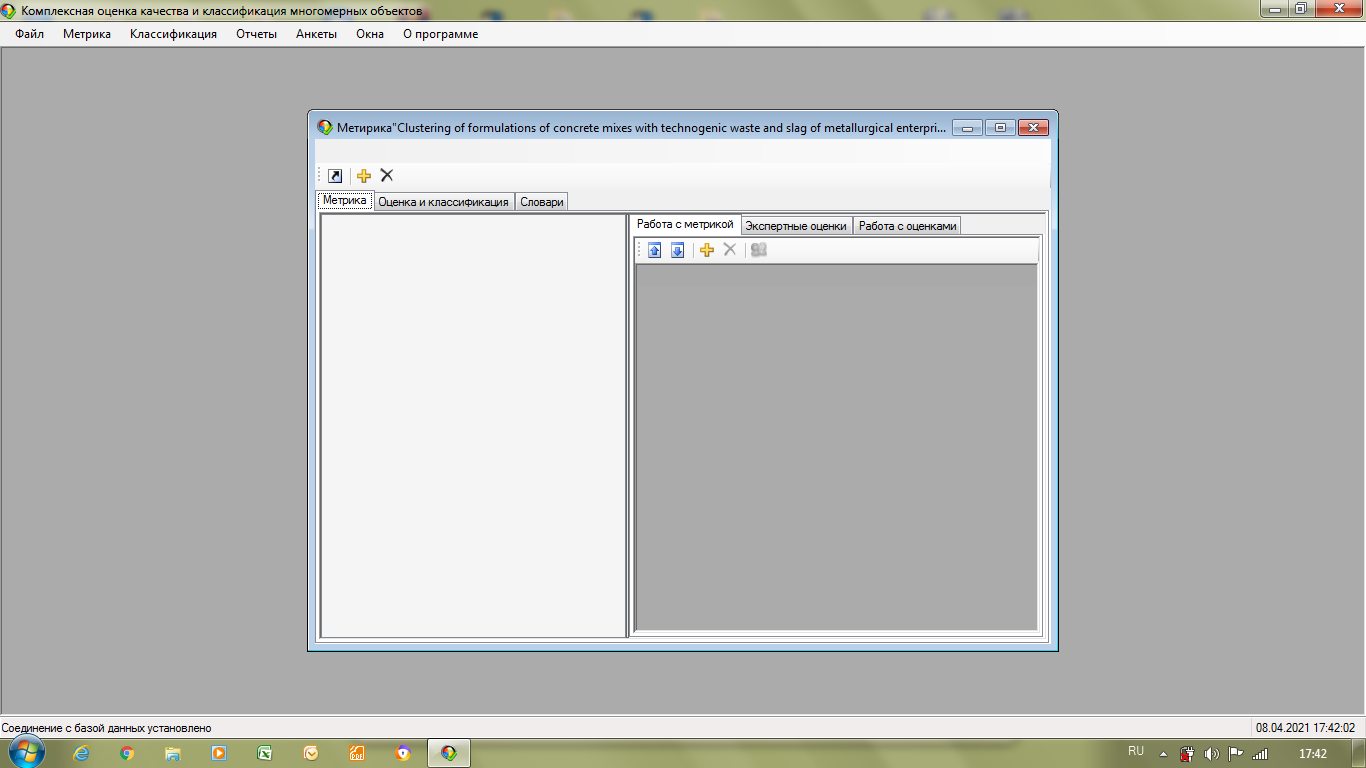
\includegraphics[width=0.8\textwidth]{image8}

Fig. 1- Program interface ""Comprehensive quality assessment and
classification of multidimensional objects"

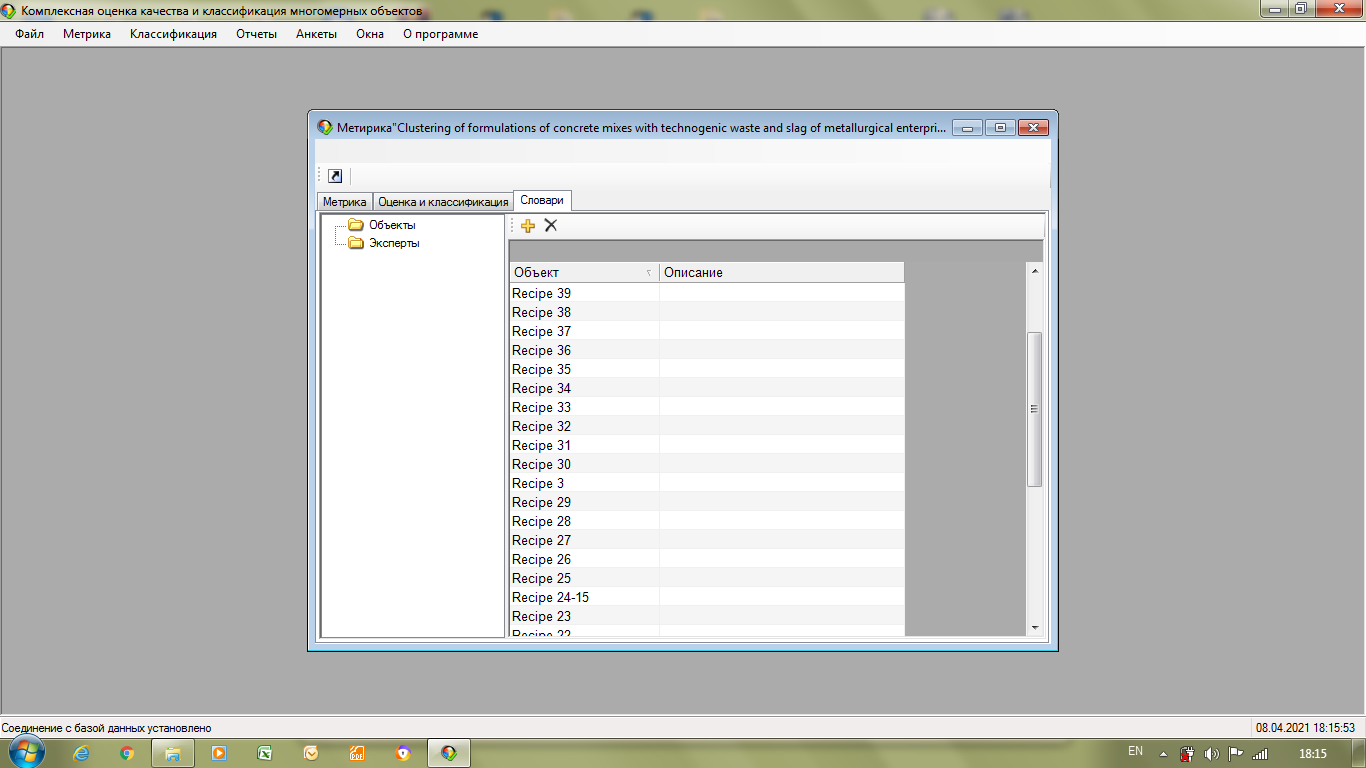
\includegraphics[width=0.8\textwidth]{image9}

Fig. 2 - Shows the input of metrics for compounding concrete mixtures

As a result of the program, the distribution of formulations of concrete
mixtures of Table 1, Figure 3 was obtained. In each cluster there are
recipes that are closest in terms of metrics.

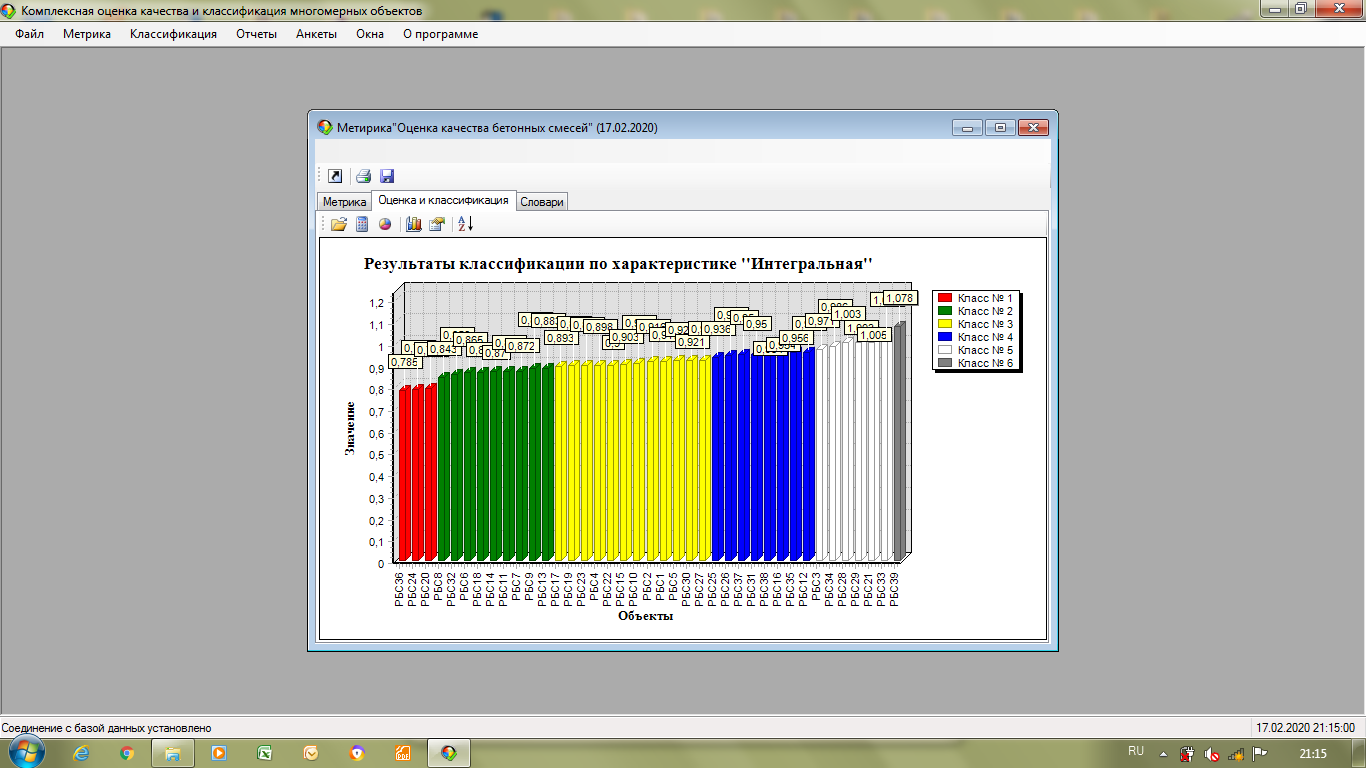
\includegraphics[width=0.8\textwidth]{image10}

Fig. 3- Clustering of concrete mix formulations

From the clustering result obtained, it can be seen that the
formulations of concrete mixtures are distributed in 6 clusters. In each
cluster there are formulations of concrete mixtures with the closest
characteristics in composition and strength. The formulations of
concrete mixtures with low strength indicators are located in clusters
1-4. Table 2 shows the formulations, the composition of concrete
mixtures with the highest strength indicators of 5 and 6 clusters.

Table 2. Recipe of cluster 5-6

\begin{longtable}[]{@{}
  >{\raggedright\arraybackslash}p{(\columnwidth - 10\tabcolsep) * \real{0.1486}}
  >{\raggedright\arraybackslash}p{(\columnwidth - 10\tabcolsep) * \real{0.1629}}
  >{\raggedright\arraybackslash}p{(\columnwidth - 10\tabcolsep) * \real{0.1812}}
  >{\raggedright\arraybackslash}p{(\columnwidth - 10\tabcolsep) * \real{0.1449}}
  >{\raggedright\arraybackslash}p{(\columnwidth - 10\tabcolsep) * \real{0.1631}}
  >{\raggedright\arraybackslash}p{(\columnwidth - 10\tabcolsep) * \real{0.1992}}@{}}
\toprule\noalign{}
\begin{minipage}[b]{\linewidth}\raggedright
Cluster №
\end{minipage} & \begin{minipage}[b]{\linewidth}\raggedright
№ recipes
\end{minipage} & \begin{minipage}[b]{\linewidth}\raggedright
Ravr.сompr.

Mpa
\end{minipage} & \begin{minipage}[b]{\linewidth}\raggedright
ash

g/\%
\end{minipage} & \begin{minipage}[b]{\linewidth}\raggedright
Metall. Slagg/\%
\end{minipage} & \begin{minipage}[b]{\linewidth}\raggedright
bauxite sludge

g/\%
\end{minipage} \\
\midrule\noalign{}
\endhead
\bottomrule\noalign{}
\endlastfoot
\multirow{6}{*}{5} & RBS3 & 8.32 & & & 674/5 \\
& RBS34 & 8.18 & & & 842/7 \\
& RBS28 & 9 & 337/2.5 & 798/6 & 505/4 \\
& RBS29 & 10 & 337/2.5 & 1596/12 & \\
& RBS33 & 9.1 & 164/1.3 & & 1685/13 \\
& RBS21 & 9.74 & 328/2.5 & 798//6 & 246/2 \\
6 & RBS39 & 22.3 & 505/4 & 1197/9.2 & 337/2.5 \\
\end{longtable}

\textbf{Methods and materials}. As a software tool for clustering
concrete mix formulations, we use the DBSCAN clustering algorithm
{[}4-11{]}.

DBSCAN (Density-based spatial clustering of applications with noise), a
density algorithm for spatial clustering with the presence of noise), as
the name implies, operates with data density.

We use the same data as in {[}1{]}.Ideally, DBSCAN can achieve good
results, but it\textquotesingle s not worth hoping for. Many versions of
the algorithm are able to work from cluster to cluster.

At the same time, the algorithm considers clusters as high-density areas
separated by low-density areas.

Because of this, clusters obtained in DBSCAN come in any shape, unlike
k-means, which assume that clusters are convex.

In practice, an important component of DBSCAN is a cluster consisting of
a set of core samples, "each of which is close to each other (measured
using some distance measurement measure) and a set of non-core samples
that are close to the core sample (but are not core samples themselves)"
{[}4{]}.

2 parameters are important for the DBSCAN algorithm: min\_samples and
eps, high min\_samples or lower eps, provide the high density necessary
for cluster organization.

The algorithm is formed in this way:

1. All points are marked as core, boundary or noise;

2. Interference will be eliminated;

3. The face between all the main points located inside at the distance
of the Eps parameter from each other is marked;

4. Each group is placed in a separate cluster;

5. The boundary points of one of the clusters associated with this
boundary point are specified.

At the same time, the base sample is part of a cluster, a sample that is
not a core sample, and exists, at a distance of eps from any core
sample, is considered an anomaly of the algorithm.

The algorithm executed (DensitybasedClusteringAlgorithm) allows the
cluster to grow until the density in the neighboring cluster exceeds a
certain threshold.

The DBSCAN algorithm is deterministic, always generating the same
clusters when providing the same data in the same order. However, the
results may differ if the data is provided in a different order. First,
even though core samples will always be assigned to the same clusters,
the labels of these clusters will depend on the order in which these
samples occur in the data. Secondly, and more importantly, the clusters
to which the non-core samples are assigned may differ depending on the
order of the data.

The clustering algorithm is effective when, as a rule, the "compactness
hypothesis" can be implemented, while splitting objects into classes,
the distances between objects from the same class
(intra-clusterdistances) will be less than some value
ϵ\textgreater0�\textgreater0, and between objects from different classes
(cross-clusterdistance) will be greater than ϵ�.

For our case, a table of distances between classes is formed in Figure
4.

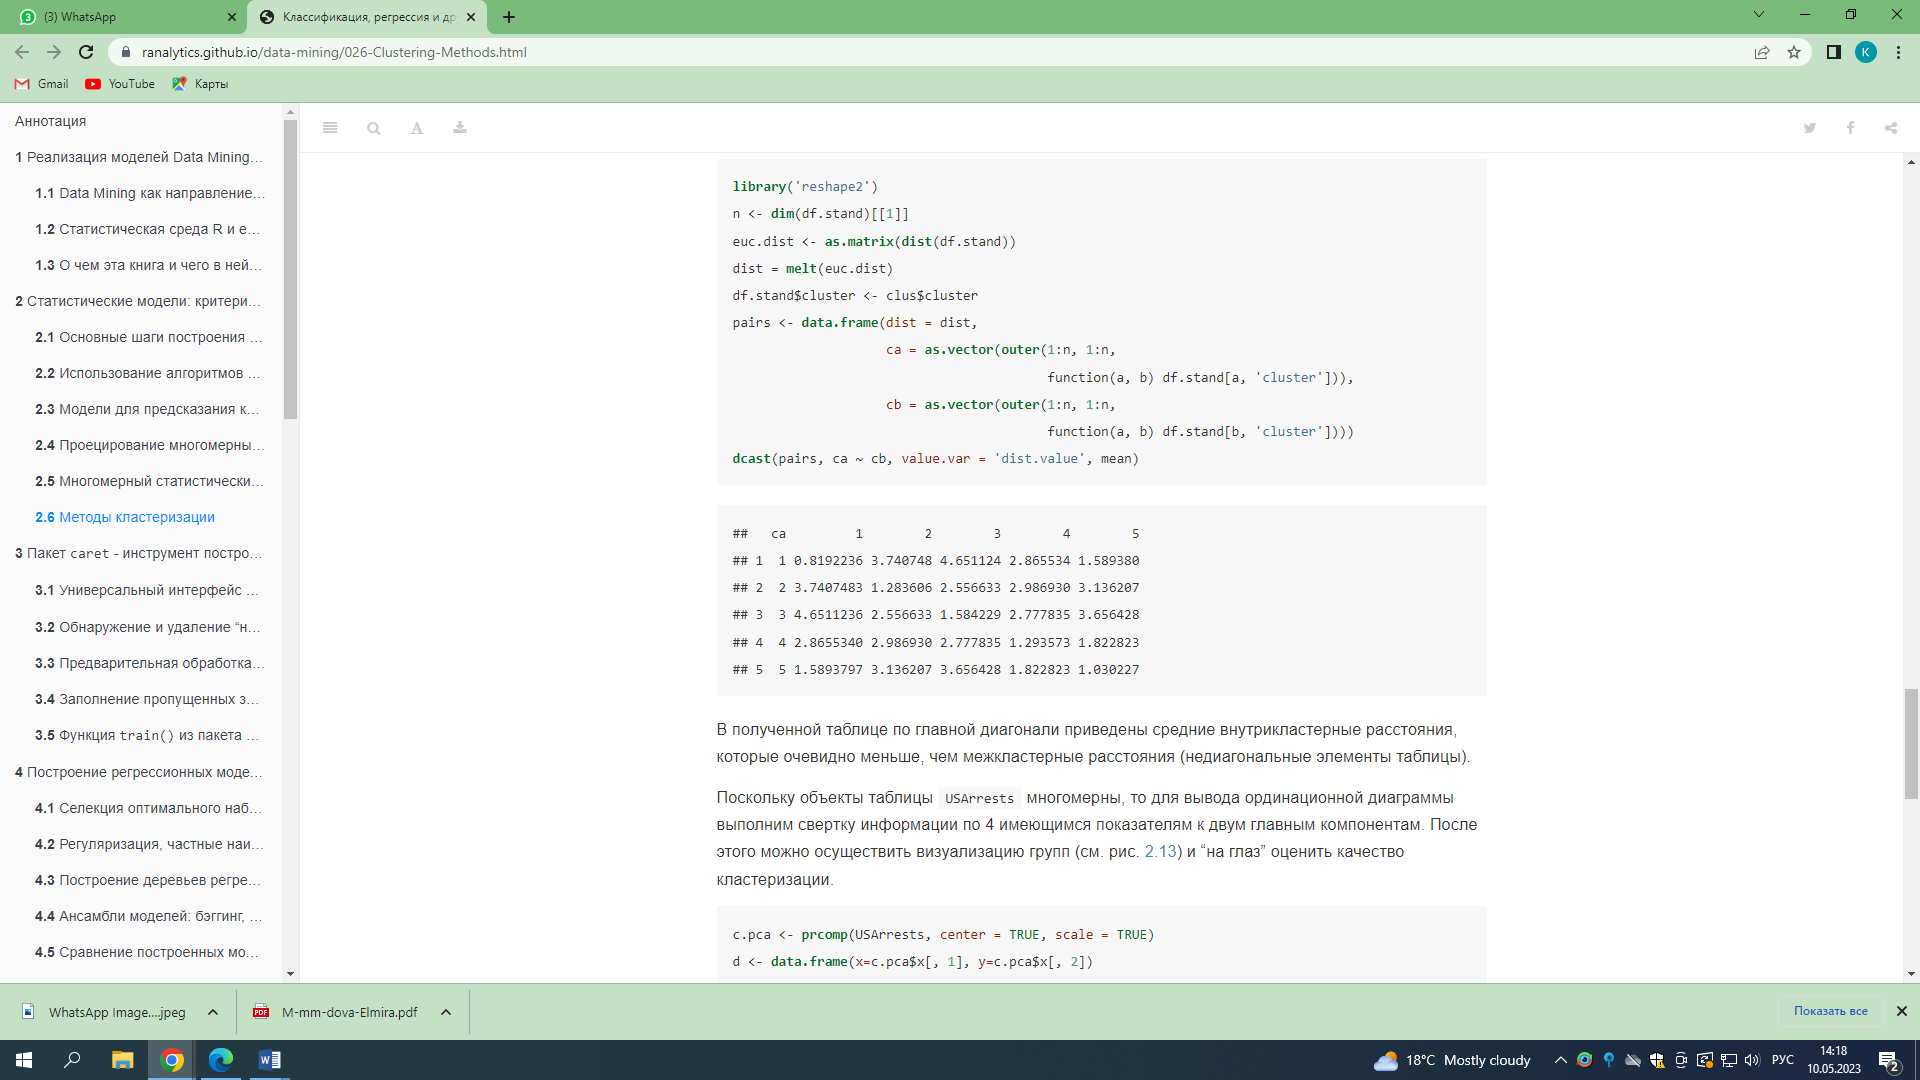
\includegraphics[width=0.8\textwidth]{image11}

Fig.4 - Table of distances between classes

From Figure 5, we see that the average intracluster distances are
significantly smaller than the intercluster distances.

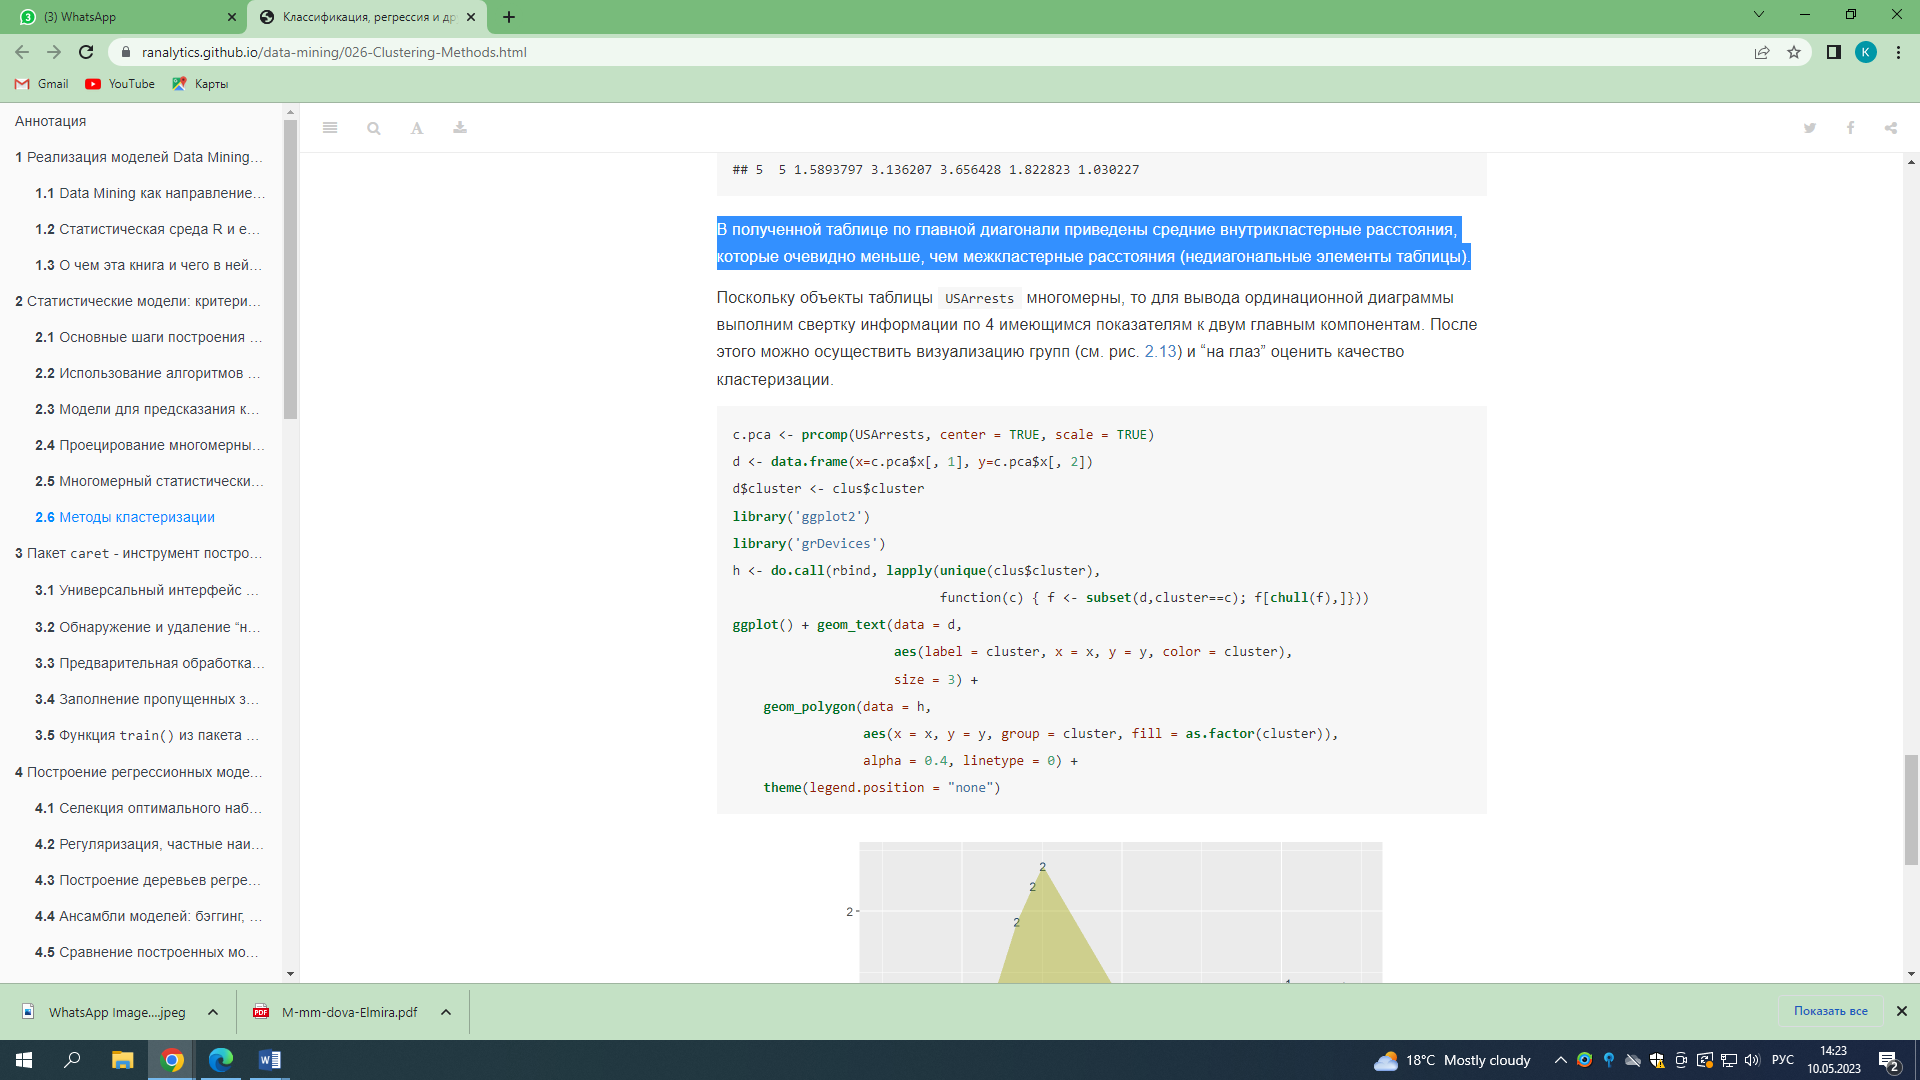
\includegraphics[width=0.8\textwidth]{image12}

Fig. 5 - Dependencies of distances inside and outside clusters

As a result, using the DBSCAN algorithm, the distribution of concrete
mix formulations by class is obtained, as shown in Figure 6.

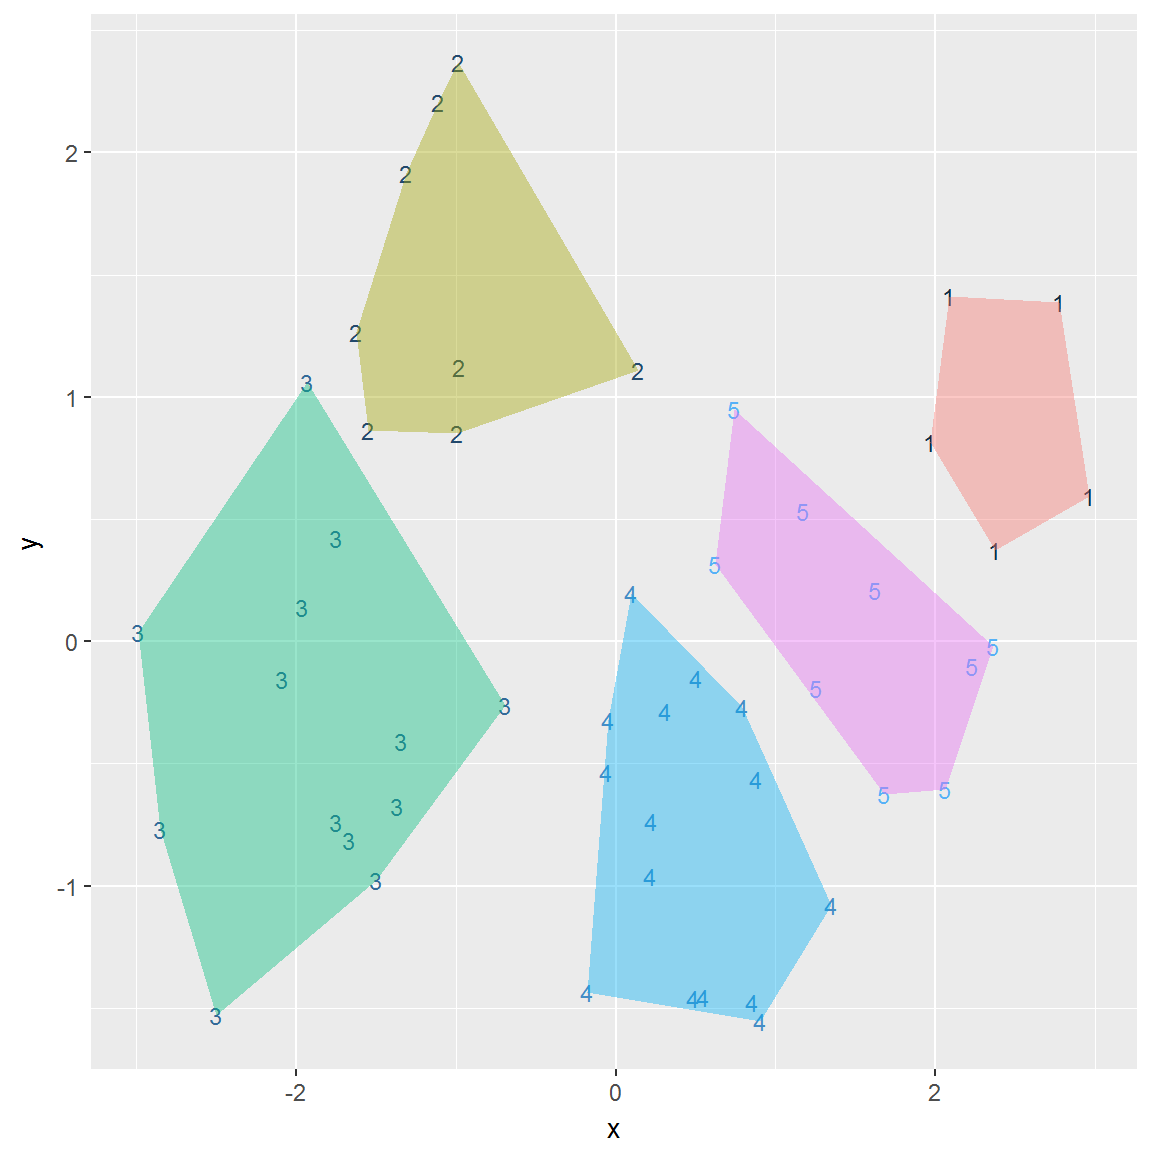
\includegraphics[width=0.8\textwidth]{image13}

Fig. 6 - Results of the distribution of concrete mix recipe by class

Figure 7 shows the clustering of concrete mix formulations.

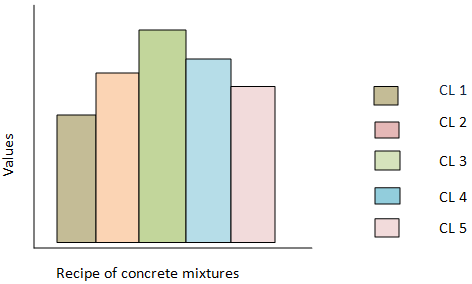
\includegraphics[width=0.8\textwidth]{image14}

Fig. 7 - Distribution of concrete mix formulations by clusters

\textbf{Discussion and results}. As can be seen from Figure 7, all the
formulations of concrete mixtures are combined into 5 clusters. The
largest is cluster 3, the smallest is cluster 1.

The task of describing in detail which formulations of concrete mixtures
were included in each cluster was not set.

Clustering technology using datamining is quite complex, the difficulty
lies in the uncontrolled decision-making process. It is not completely
clear whether the correct solution has been achieved.

"Deep artificial neural networks are very good at classification, but
clustering is still an open question"{[}2{]}.

\textbf{Conclusions.} We see that DataMining is quite a promising tool
for clustering, including formulations of concrete mixtures. Although
the results leave much to be desired compared to those previously
obtained in {[}1{]}, nevertheless, with fairly constant machine learning
and training, there is a potential prospect that we will get good
clustering results. In the future, we plan to use one of the software
tools presented above for clustering man-made waste of the Pavlodar
region.

\textbf{Referenses}

1. Akishev K and other. Mathematical formulation and the problem
solution of clustering recipes of concrete mixtures using technogenic
waste waste and slags of metallurgical enterprises.-- Метаllurjia. -
2022. - 61(1)213-216. Zagreb, p.321.

2. Electronicresource
:URL:\href{https://www.google.com/url?sa=t\&source=web\&rct=\%20j\&url=https://trends.rbc.ru}{https://www.google.com/url?sa=t\&source=web\&rct=
j\&url=https://trends.rbc.ru}/trends/amp/news/61b359739a7947c7376ef7ce\&ved
=2ahUKEwi8t6 uloOj-AhWPxosKHaboDG4QFnoECCAQAQ\&usg=
AOvVaw2QeUcHkOYOZ3RdPy3Sttjx -Date of application 12.05.2023.

3. Electronic
resource:URL:\url{https://cyberleninka.ru/article/n/analiz-i-klassifikatsiya-algoritmov-klasterizatsii}
- Date of application 12.05.2023.

4. Electronic
resource:URL:\url{https://etu.ru/assets/files/nauka/}dissertacii /2009
/SIElizarov.doc. -date of application 12.05.2023.

5. Electronicresource:
URL:\url{https://elibrary.ru/item.asp?id=45420956} - Date of application
12.05.2023.

6. Electronicresource :URL:\url{https://habr.com/ru/articles/322034/}
-Date of application 12.05.2023.

7. Electronic resource:URL:
\url{http://pzs.dstu.dp.ua/DataMining/cluster/bibl/\%25}D0\% 9A
\%D0\%9B\%D0\%90\%D0\%A1\%D0\%A2\%D0\%95\%D0\%A0\%D0\%98\%D0\%97\%D0\%90\%D0\%A6\%D0\%98\%D0\%AF\%20\%D0\%9E\%D0\%91\%D0\%AA\%D0\%95\%D0\%9A\%D0\%A2\%D0\%9E\%D0\%92\%20\%D0\%A1\%20\%D0\%9F\%D0\%9E\%D0\%9C\%D0\%9E\%D0\%A9\%D0\%AC\%D0\%AE\%20\%D0\%90\%D0\%9B\%D0\%93\%D0\%9E\%D0\%A0\%D0\%98\%D0\%A2\%D0\%9C\%D0\%90\%20DBSCAN.pdf
- Date of application 12.05.2023{]}

8. Electronicresource: URL:
\url{https://www.math.spbu.ru/SD_AIS/documents/2014-05-341/2014-05-tw11.pdf}
-Date of application 12.05.2023.

9. Electronicresource:URL:
\url{https://core.ac.uk/download/pdf/196226625.pdf} - date of
application 12.05.2023.

10. Electronic resource :URL: Ortiz-Arroyo D. Discovering Sets of Key
Players in Social Networks // Computational Social Networks Analysis. --
2010 -- C. 27-47 {[}Date of application 12.05.2023.

11.Electronic resource:URL:
\href{https://kpfu.ru/portal/docs/F_1980845423/161_3\%20_phys\%20_mat_8.pdf}{https://kpfu.ru/portal/docs/F\_1980845423/161\_3
\_phys \_mat\_8.pdf} - Date of application 12.05.2023.

\emph{\textbf{Information about the authors}}

Akishev Karshyga Maksutovich, Candidate of Technical Sciences, Ass.
Professor, Department of "Information Technology", Kazakh University of
Technology and Business, Astana, Republic of
Kazakhstan:email:akmail04cx@mail.ru

Karpov Valery Ivanovich, Doctor of Technical Sciences, Professor,
Department of Information Technology, Moscow State University of
Technology and Management named after K.G. Razumovsky, Moscow, Russia
:email:Vikarp@mail.ru

Akisheva Lenara Karshygaevna, 7th grade student of Nazarbayev
Intellectual School, Astana, Republic of Kazakhstan email:LK@mail.ru

Tulegulov Amandos Dabysovich, Ph.D., Ass. Professor, Head of the
Department of "Information Technology", Kazakh University of Technology
and Business, Astana, Republic of Kazakhstan email:tud62@yandex.ru

\emph{\textbf{Сведения об авторах}}

Акишев Каршыга Максутович, к.т.н., асс. профессор, кафедра
«Информационные технологии», Казахский университет технологии и бизнеса,
г. Астана, Республика Казахстан: email:akmail04cx@mail.ru

Карпов Валерий Иванович, доктор технических наук, профессор, кафедра
«Информационные технологии» Московский Государственный универститет
технологии и управления имени К.Г. Разумовского,г. Москва,
Россия:email:Vikarp@mail.ru

Акишева Ленара Каршыгаевна, ученица 7 классса Назарбаев Интеллектуальная
школа, г. Астана, Республика Казахстан LK@mail.ru

Тулегулов Амандос Дабысович, к.ф.м.н., асс. профессор, зав. кафедрой
«Информационные технологии», Казахский университет технологии и бизнеса,
г. Астана, Республика Казахстан: tud62@yandex.ru

\textbf{SRSTI 52-77; 003.11}

\begin{quote}
\textbf{EXPLORING THE USE OF ELECTRONIC MEDICAL RECORDS FOR PATIENTS}
\end{quote}

\textbf{G.Z.Ziyatbekova\textsuperscript{1,2*}, M.K.
Omirzak\textsuperscript{2}, G.Z. P.Kisala\textsuperscript{3}}

\textsuperscript{1}RSE Institute of Information and Computational
Technologies MSHE RK CS,

Almaty, Kazakhstan, \textsuperscript{3} Lublin Technical University,
Poland,

\textsuperscript{2}Al-Farabi Kazakh National University, Almaty,
Kazakhstan,

e-mail:
\href{mailto:ziyatbekova@mail.ru}{\nolinkurl{ziyatbekova@mail.ru}}

\textbf{Abstract.} The article is devoted to the study of the
information system of electronic medical records of patients in order to
improve the work of the ambulance service. Scientific research in the
field of medicine is given. This article discusses medical information
systems and the principles of their functioning. It also shows the
process of effective work due to medical information system. A
user-friendly interface is used. The following functions are touched
upon: elimination of paperwork, transition to electronic system,
additional medical services. All available methods are presented, which
are the key factors in optimizing all medical processes. Also considered
options for modeling and system development, taking into account all the
relevant issues of automation of medical information systems. The
developed information complex can be used both in polyclinics and in
pharmacies, as well as individually for patients. The article deals with
the study of electronic medical records system. In this work developed a
medical information system and ER system as an application. The
possibility of processing, storing and conveniently viewing the created
data system is provided.

\textbf{Key words:} ambulance, electronic medical record, medicine,
medicine, website.

\textbf{ПАЦИЕНТТЕРДІҢ ЭЛЕКТРОНДЫ МЕДИЦИНАЛЫҚ ЖАЗБАЛАРЫН}

\textbf{ҚОЛДАНУ МҮМКІНДІКТЕРІН ЗЕРТТЕУ}

\textbf{Г.З.Зиятбекова\textsuperscript{1,2*},
P.Kisala\textsuperscript{3}, М.Қ.Өмірзақ\textsuperscript{2}}

\textsuperscript{1}Қазақстан Республикасы Ғылым және жоғары білім
министрлігі Ақпараттық және есептеуіш технологиялар институты, Алматы,
Қазақстан, \textsuperscript{3}Люблин техникалық yниверситеті, Польша,
\textsuperscript{2}әл-Фараби атындағы Қазақ ұлттық университеті, Алматы,
Қазақстан,

e-mail:
\href{mailto:ziyatbekova@mail.ru}{\nolinkurl{ziyatbekova@mail.ru}}

\textbf{Аннотация.} Мақала жедел жәрдем жұмысын жақсарту мақсатында
пациенттердің электрондық медициналық картасын жүргізудің ақпараттық
жүйесін зерттеуге арналған. Медицина саласындағы ғылыми зерттеулер
келтірілген. Бұл мақалада медициналық ақпараттық жүйелер және олардың
жұмыс істеу принциптері қарастырылады. Медициналық ақпараттық жүйенің
арқасында тиімді жұмыс процесі де көрсетілген. Пайдаланушыға ыңғайлы
интерфейс қолданылды. Келесі функциялар қозғалады: қағазбастылықты жою,
электрондық жүйеге көшу, қосымша медициналық қызметтер. Қазіргі уақытта
барлық медициналық процестерді оңтайландырудың негізгі факторлары болып
табылатын барлық қол жетімді әдістер ұсынылған. Сондай-ақ, медициналық
ақпараттық жүйелерді автоматтандырудың барлық өзекті мәселелерін ескере
отырып, жүйені модельдеу және әзірлеу нұсқалары қарастырылған. Әзірленіп
жатқан ақпараттық кешенді емханаларда да, дәріханаларда да, пациенттер
үшін де жеке пайдалануға болады. Мақалада электронды медициналық
жазбалар жүйесін зерттеу қарастырылады. Бұл жұмыста қосымша ретінде
медициналық ақпараттық жүйе және жедел жәрдем жүйесі жасалды. Құрылған
деректер жүйесін өңдеу, сақтау және ыңғайлы қарау мүмкіндігі
қарастырылған.

\textbf{Түйін сөздер:} жедел жәрдем, электронды медициналық жазба,
медицина, дәрі-дәрмек, веб-сайт.

\textbf{ИССЛЕДОВАНИЕ ВОЗМОЖНОСТЕЙ ИСПОЛЬЗОВАНИЯ ЭЛЕКТРОННЫХ МЕДИЦИНСКИХ
КАРТ ПАЦИЕНТОВ}

\textbf{Г.З. Зиятбекова\textsuperscript{1,2*},
P.Kisala\textsuperscript{3}, М.Қ. Өмірзақ\textsuperscript{2}}

\textsuperscript{1}Институт информационных и вычислительных технологий
КН МНВО РК, Алматы,

Казахстан, \textsuperscript{3}Люблинский технический yниверситет, Польша

\textsuperscript{2}Казахский национальный университет имени аль-Фараби,
Алматы, Казахстан,

e-mail:
\href{mailto:ziyatbekova@mail.ru}{\nolinkurl{ziyatbekova@mail.ru}}

\textbf{Аннотация.} Статья посвящена изучению информационной системы
ведения электронной медицинской карты пациентов с целью улучшения работы
скорой помощи. Приведены научные исследования в области медицины. В
данной статье рассматриваются медицинские информационные системы и
принципы их функционирования. Также показан процесс эффективной работы
благодаря медицинской информационной системе. Использован удобный
интерфейс. Затрагиваются следующие функции: устранение бумажной
волокиты, переход на электронную систему, дополнительные медицинские
услуги. В настоящее время представлены все доступные методы, которые
являются ключевыми факторами оптимизации всех медицинских процессов.
Также рассмотрены варианты моделирования и разработки системы с учетом
всех актуальных вопросов автоматизации медицинских информационных
систем. Разрабатываемый информационный комплекс можно использовать как в
поликлиниках, так и в аптеках, а также индивидуально для пациентов. В
статье рассматривается исследование системы электронных медицинских
карт. В данной работе разработана медицинская информационная система и
система Скорой помощи в качестве приложения. Предусмотрена возможность
обработки, хранения и удобного просмотра созданной системы данных.

\textbf{Ключевые слова:} скорая помощь, электронная медицинская карта,
медицина, лекарства, веб-сайт.

\textbf{Introduction.} There are many automated control systems designed
to automate the work of emergency stations and departments, but they are
mostly expensive tools and require expensive equipment and skilled
professionals. This raises the challenge of creating an automated
workstation for an ambulance dispatcher "ambulance". In recent years,
not only has the number of computer equipment in medical institutions
increased, but also the quality of communication has improved
significantly, allowing the system to move to a web-based platform. The
complexity of managing and maintaining the current version of the system
does not allow it to be used in small, private and remote medical
institutions, which makes it difficult to automate the exchange of
information. The transition to the Web platform will allow to expand the
range of medical organizations and implement the system {[}1{]}.

Theoretical methods and research analysis were developed as a research
method. Theoretical methods of research allow you to systematize
information, reveal the nature of various phenomena and objects, to
identify relationships between processes. 7 main problems and 7
principles of their solution:

1.The lack of the principle of normative regulation and incentives to
conduct EMC.

2.Problems and principles of integrated document management in medicine.

3. legal significance

4. ensuring of reliability and rules of collective work

5. defining the right of access to electronic medical document

6. structuring and standardization of medical information for electronic
exchange of medical documents

7. principle of systematic sufficiency

According to electronic medical records management, when developing new
rules, they should include balanced requirements for technical means
used in combination with carefully considered organizational measures.

Development of a web application for the ambulance medical information
system, which allows to automate the work of an ambulance dispatcher in
private and remote municipal health care facilities with the ability to
work remotely. It is designed to increase the productivity of ambulance
workers and reduce processing and data entry time. It also provides
various opportunities for immediate contact with ambulance staff.

\textbf{Materials and methods.} The general system and the medical
laboratory information system can be integrated with modern medical
equipment. In addition, medical IS make it possible to promptly bring
general statistics about the state of health of the population to
municipal authorities and other state institutions. In this connection,
the electronic medical record is used.

The main goals of the electronic medical record:

\begin{itemize}
\item
  To collect and store electronically as much information as possible
  about a specific person\textquotesingle s health;
\item
  Promptly provide access to this information to authorized medical
  workers, the individual himself and his authorized representatives in
  the most convenient and accessible form for a particular user;
\item
  Creation of specialized electronic services based on this information,
  aimed at medical personnel, at the individual himself, and providing
  improved safety and quality of medical care, as well as improved
  quality of life and health of citizens {[}2{]}.
\end{itemize}

These software packages offer the optimal solution for preparing
reporting documents and, in the opinion of many users, are a necessary
component of any ambulance station. But not every ambulance station
allows for the implementation and maintenance of these software
packages. As before, the main problem of widespread implementation of
these systems and their analogues remains the limitation of financial
availability of these programs at the municipal level.

The next step is to describe the Web technologies for creating an
electronic medical record information system for patients. The
server-side programming language for Web applications is Python. Python
is an interpreted, interactive, object-oriented programming language. It
is created in the django framework to create web applications with
little code. A database is used to systematically store an array of data
collected and easily accessible by an authorized user. It is stored to
retrieve the necessary data from the database as needed. Therefore, the
database was implemented using a SQLite database. The client part and
GUI were implemented using JavaScript language, which allows for a
user-friendly and responsive interface. This allows users to access and
interact with basic data in the database. These actions can range from
simple data querying to defining database schemas that radically affect
the database structure.

\textbf{Results and discussion.} According to electronic medical
records, when new regulations are developed, they must include balanced
requirements for the technical means used, combined with carefully
considered organizational measures (Fig. 1).

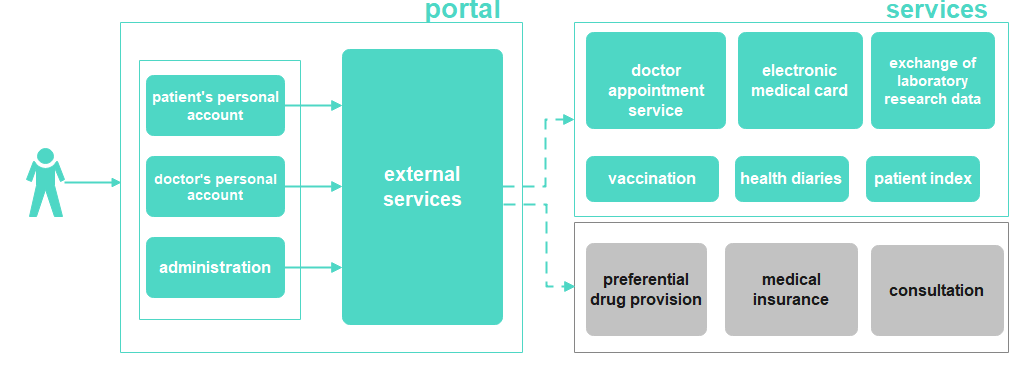
\includegraphics[width=0.8\textwidth]{image15}

Figure 1 - Vision for the medical center portal

Information system for electronic medical records of patients before
compiling the technical part of the web-application, it is necessary to
define the requirements to the web-application.

The following requirements apply to a web-based information system for
maintaining electronic medical records:

\begin{itemize}
\item
  Patients must be able to provide complete information;
\item
  Patients should be able to register and then log in to the system;
\item
  information about the patient, records of doctor\textquotesingle s
  visits should always be available in the personal account;
\item
  the doctor must be able to see the patient\textquotesingle s medical
  history, to make records in the medical history;
\item
  the administrator of the web application must be able to view,
  customize information about patients and doctors and arrange for the
  patient to contact the doctor.
\item
  the administrator and physicians need to have separate registration
  and login pages.
\end{itemize}

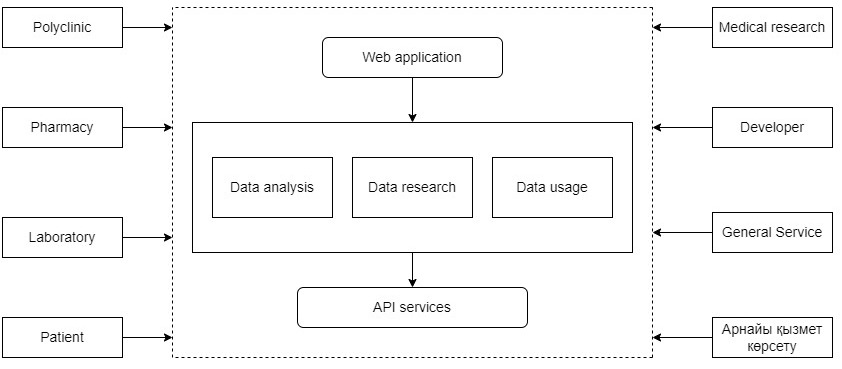
\includegraphics[width=0.8\textwidth]{image16}

Figure 2 - Medical Web Application Connection Diagram

The web-based patient application contains an electronic health record,
as described in the previous electronic health record in addition to
including other types of services(Fig. 2). This system establishes
communication with institutions that have access to internal data.
Through the outpatient clinic, pharmacy, and laboratory, certificates
issued by the doctor are indicated. The service and medical research
departments also have the ability to obtain the necessary data
{[}3-4{]}.

Each patient has a unique opportunity to receive the following
information:

\begin{itemize}
\item
  Information about the prescription written by the attending physician;
\item
  Vaccination schedule;
\item
  Information about pharmacies that provide free medications;
\item
  diagnoses;
\item
  hospitalization records.
\end{itemize}

The information received cannot be processed. For visitors to the
e-Health Passport, only training mode is available.


\includegraphics[width=0.8\textwidth]{image17}

Figure 3 - "About the ambulance"

Under the ambulance data, we can see our mission, the staff. If we click
on it, we can see information about it (Fig. 3).

The ambulance is an emergency medical service. Therefore, the emergency
medical service is of great importance in the health care system. Its
mission is to protect people\textquotesingle s health by providing
services that are affordable and meet the current professional and
technical level of emergency medical care.

Types of service we provide:

\begin{itemize}
\item
  diagnosis and emergency care;
\item
  Doctors who are invited to come to the home;
\item
  full supervision.
\end{itemize}

For more information, click on the button to see the types of services.
Long-term hospital care provides long-term care measures for patients
who are in serious condition. Specialized care is provided with full
monitoring of patients in need of medical care. Along with sleepwalking,
each place of care was also fully monitored by medical transport
{[}5-6{]}.

Providing first aid to patients in need of emergency care, through a set
of diagnostic and emergency services of a comprehensive type for those
who are referred. Median locations through house call physicians are for
regular patients in certain rural areas and patients who must be checked
regularly over a period of time {[}7-8{]}.

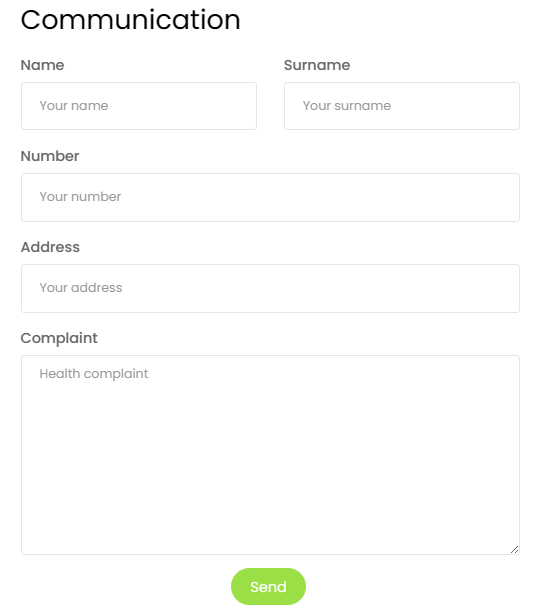
\includegraphics[width=0.8\textwidth]{image18}

\begin{quote}
Figure 4 - Emergency communication menu
\end{quote}

In the event of a specific emergency, by visiting the site, you can go
to the emergency communication menu and drop off an application (Fig.
4). The following form is required to be filled out in full.They:

\begin{itemize}
\item
  first name;
\item
  your last name;
\item
  your phone number;
\item
  letter.
\end{itemize}

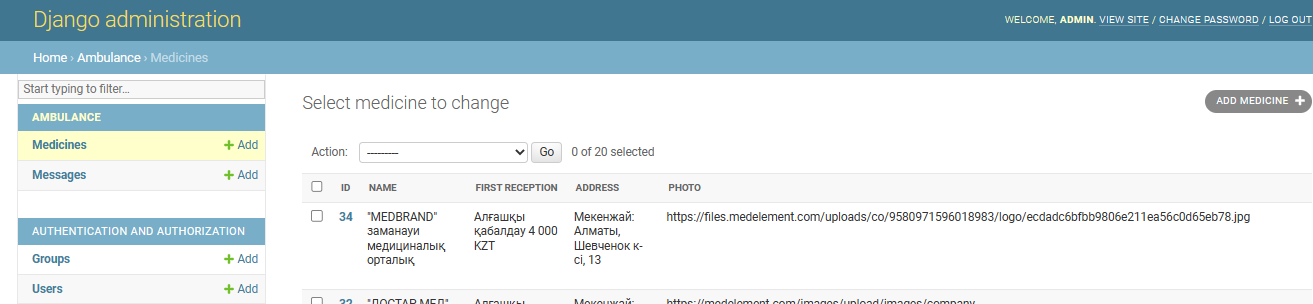
\includegraphics[width=0.8\textwidth]{image19}

Figure 5 - Representation of saving in the database

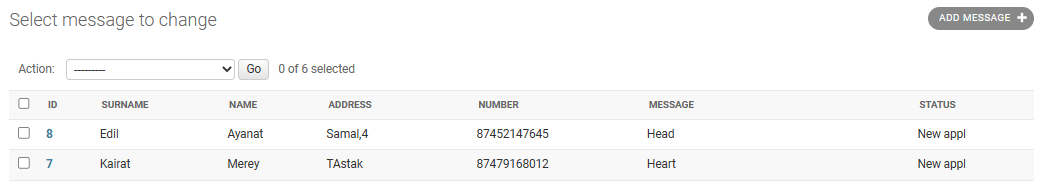
\includegraphics[width=0.8\textwidth]{image20}

Figure 6 - Storing in the database

The completed emergency form goes into the database.

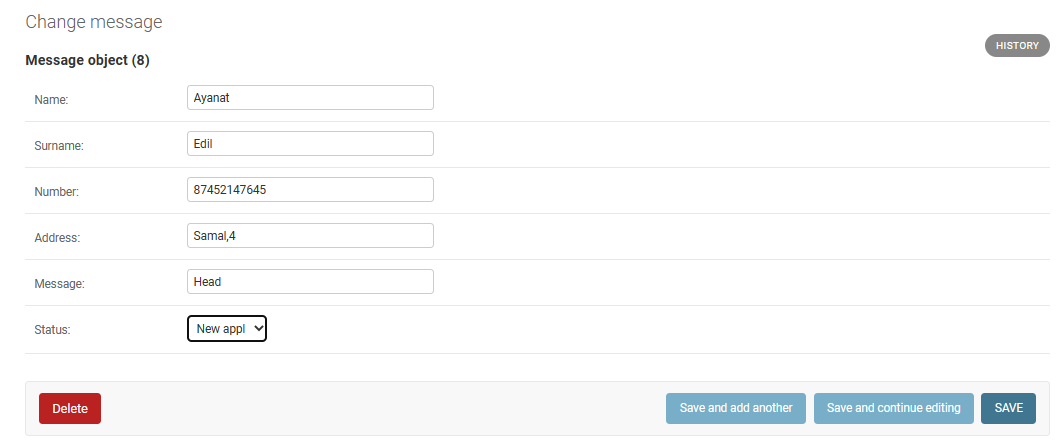
\includegraphics[width=0.8\textwidth]{image21}

Figure 7 - Changing the status in the database

You can change the status of incoming data in the database. Also saves
again, changing the status(Fig. 5-6).

You can change the status in the data. The status consists of:

\begin{itemize}
\item
  new request;
\item
  sent;
\item
  completed;
\item
  invalid application.
\end{itemize}

For example, highlight the status "sent" and click the "Save" button. At
this point, the status of the data sent to the database changes (Fig.
8).

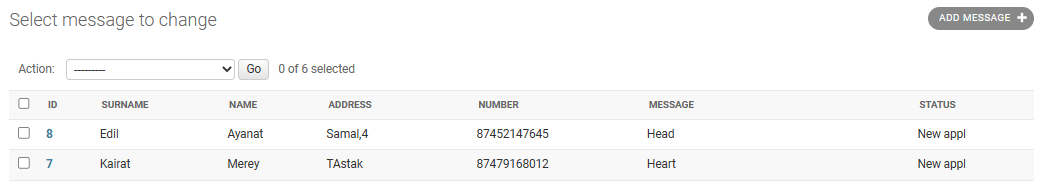
\includegraphics[width=0.8\textwidth]{image20}

Figure 8 - Database when changing and saving the status

The results of the study show that the web application, working through
a medical information system, has the ability to communicate with
patients. As a result of the work the following results were achieved:

- Subject area analysis and problem statement;

- analysis of existing software for the automation of emergency medical
care;

- definition of requirements to the developed software.

The sent protocol is processed in the database and is in the row of new
letters. In this way, patients can report their illness in advance. This
will not only eliminate paperwork at medical centers, but also make the
work of medical professionals easier. As a result, efficiency is
increased and the quality of work is improved through possible
implementation in remote and small medical centers.

\textbf{Conclusion.} The module was developed using web-programming
technologies. The client part and the graphical interface were
implemented with the help of JavaScript language, which allowed to get a
convenient and responsive interface. The server part was implemented in
python with the help of a framework.

The result of the work is a full-fledged web application with the
possibility of implementation in remote and small medical institutions.

An outpatient record in any paper form, that is, a
patient\textquotesingle s records of illness, treatment, are compiled by
a person since childhood and are updated over time. However, the most
well-known negative properties of paper documents are obsolescence and
high probability of loss. That is why now, in the course of information
technology development, it is more and more common to develop electronic
versions of such documents.

The EMR can be used in any medical facility. When using this system, all
processes that take place will be exactly the same as when an outpatient
record is created and maintained. That is, the administrator of the
institution first registers the patient, and then the
patient\textquotesingle s personal account appears. Then personal
meetings are held with the doctor, as a result of which the doctor
registers the necessary records - diagnosis, prescriptions for
treatment, necessary documents in the EMR, and information about this
record appears in the personal office of both the patient and the doctor
and administrator, in the form of an EMR record. These appointments will
be held and the patient\textquotesingle s EMR will be filled out.

While doing this article, I delved into Python and SQLite databases and
programming languages. In doing so, choosing the necessary languages to
create the site, it stopped at the pros and cons of the language.

\textbf{References}

\begin{enumerate}
\def\labelenumi{\arabic{enumi}.}
\item
  Abushaev sh. t. how to buy mis? Practical recommendations for heads of
  health care and general medicine -- how to improve medical information
  systems //medicine and information technologies. 2020. №3. P. 47.
\item
  Galieva G. B., Iunbaeva a.m., Urazhanova N. zh. on the special
  education of children for the new and new medical care in Taldykorgan.
  - Youth School, No. 2 (49). - 2019. - 2p.
\item
  Nadinia Davis: Foundations of Health Information Management --
  5\textsuperscript{th} Edition, ISBN: 9780323674966, 2019.
\item
  Yassine Maleh, Ahmed A. Abd El-Latif, Kevin Curran, Patrick Siarry:
  Computational Intelligence for Medical Internet of Things (MIoT)
  Applications -- 1\textsuperscript{st} Edition, 2022
\item
  Boris Kobrinksy. Intelligent systems for medicine: Retrospective and
  perspective // Sixth International Scientific Conference ``Intelligent
  Information Technologies for Industry'' (IITI'22). 2022.
\item
  Zarubina T. V., Kobrinsky B. A., Belonosov S. S. and Dr. Medical
  Informatics: teacher / under the office. Ed. T. V. Zarubinoy, B. A.
  Kobrinsky. 2-e izd. M.: Geotar-Media, 2022.
\item
  Faezeh Afzali,Yunes Jahani, Fatemeh Bagheri \& Reza khajouei, BMC
  Medical Informatics and Decision Making, 2021.
\item
  Gail Baura: Medical Device Technologies -- 2\textsuperscript{nd}
  Edition, ISBN: 9780128119846, 2020.
\end{enumerate}

\emph{\textbf{Information about the authors}}

Ziyatbekova Gulzat Ziyatbekkyzy -- PhD, Acting Associate Professor NAO
Al-Farabi Kazakh National University; Senior Researcher at the RSE
Institute of Information and Computational Technologies of the National
Academy of Sciences of the Republic of Kazakhstan;
\href{mailto:ziyatbekova@mail.ru}{\nolinkurl{ziyatbekova@mail.ru}};

Omirzak Merey Kairatkyzy -- graduate student at Al-Farabi Kazakh
National University; kayratovnam@mail.ru.

Piotr Kisala -- PhD, Associate Professor Lublin Technical University,
Poland; \href{mailto:p.kisala@pollub.pl}{\nolinkurl{p.kisala@pollub.pl}}

\emph{\textbf{Сведения об авторах}}

Зиятбекова Гулзат Зиятбеккызы -- PhD, и.о. доцента НАО Казахского
национального университета имени аль-Фараби; старший научный сотрудник
Института Информационных и вычислительных технологий КН МНВО РК;
\href{mailto:ziyatbekova@mail.ru}{\nolinkurl{ziyatbekova@mail.ru}};

Өмірзақ Мерей Қайратқызы -- магистрант НАО Казахского национального
университета имени аль-Фараби, kayratovnam@mail.ru;

Piotr Kisala -- PhD, доцент Люблинского технического университета,
Польша; p.kisala@pollub.pl

\textbf{ДОЛЖНА БЫТЬ СТАТЬЯ ЖАМАНГАРИНА С.}

\textbf{ҒТАХР 65.55.37}

\textbf{ХОЛЕКАЛЬЦИФЕРОЛДЫҢ ОЛИГОҚАНТПЕН СУДА ЕРИТІН}

\textbf{КЕШЕНІН АЛУ}

\textbf{С. Фазылов\textsuperscript{1*}, O.Нүркенов\textsuperscript{1},
A. Искинеева\textsuperscript{2}, A.Мұстафаева\textsuperscript{2},}

\textbf{И. Пустолайкина\textsuperscript{3}, А.
Сарсенбекова\textsuperscript{3}, А.Свидерский\textsuperscript{4}}

\textsuperscript{1}Органикалық синтез және көмірхимиясы институты,
Қарағанды, Қазақстан,

\textsuperscript{2}С.Сейфуллин атындағы Қазақ агротехникалық
университеті, Астана, Қазақстан,

\textsuperscript{3} Е.Бөкетов атындағы Қарағанды университеті,
Қарағанды, Қазақстан,

\textsuperscript{4}Инновациялық Еуразия университеті, Павлодар,
Қазақстан,

e-mail: \href{mailto:iosu8990@mail.ru}{\ul{iosu8990@mail.ru}}

Мақалада майда еритін холекальциферолдың крахмал олигоқантымен капталған
түрін алу бойынша зерттеу нәтижелері келтірілген. Өндіріс жағдайында
ылғалды ортада майда еритін холекальциферолдың жоғары липофильділігі
және төмен ерігіштігі белгілі бір қиындықтар тудырады. Осы себепті
биофармацевтикалық және қоректік қасиеттері жақсартылған холекальциферол
дәруменінің (ХД) суда еритін түрлерін алудың технологиялық әдістерін
жасау қажеттілігі туындайды. Жүргізілген зерттеулер нәтижесінде ХД
крахмалдың олигоқантымен (бета-тұйықдекстрин, β-ТД) қапталған суда
еритін кешені алынды. Молекулалық үлгілеудің \emph{in silico}
әдістерімен ХД-дың β-ТД-мен кешендерінің клатратты түрлерінің түзілу
механизмдері зерттелді. Клатрат түзілуіндегі кристаллдың беткі қабатының
морфологиясы электронды микроскоп деректерімен әртүрлі үлкейту
жағдайында сарапталды. Термографиялық өлшеулердің нәтижелері, сондай-ақ
бастапқы және соңғы қосылыстардың салыстырмалы \textsuperscript{1}Н және
\textsuperscript{13}С ЯМР спектроскопиялық параметрлері ұсынылды.
Алынған жаңа ғылыми нәтижелер олигоқанттың гидрофобты қуысында ішкі
(инклюзивті) кешен пайда болады деген қорытынды жасауға мүмкіндік
береді.

\textbf{Түйін сөздер:} холекальциферол, функционалды тамақтану,
олигоқанттар, β-тұйықдекстрин, қосылу кешендері, клатрат

\textbf{ПОЛУЧЕНИЕ ВОДОРАСТВОРИМОГО КОМПЛЕКСА} ХОЛЕКАЛЬЦИФЕРОЛА \textbf{С
ОЛИГОСАХАРИДОМ}

\textbf{С. Фазылов\textsuperscript{1*}, O.Нуркенов\textsuperscript{1},
A. Искинеева\textsuperscript{2}, \textsuperscript{2}A.
Мустафаева\textsuperscript{2},}

\textbf{И. Пустолайкина\textsuperscript{3},
А.Сарсенбекова\textsuperscript{3}, А.Свидерский\textsuperscript{4}}

\textsuperscript{1}Институт органического синтеза и углехимии РК,
Караганда, Казахстан,

\textsuperscript{2} Казахский агротехнический университет имени С.
Сейфуллина, Астана, Казахстан,

\textsuperscript{3} Карагандинский университет имени Е.Букетова,
Караганда, Казахстан,

\textsuperscript{4}Инновационный Евразийский университет, Павлодар,
Казахстан,

e-mail: iosu8990@mail.ru

В статье представлены результаты исследования по получению
капсулированной формы жирорастворимого холекальциферола с олигосахаридом
крахмала. В производственных условиях высокая липофильность и низкая
растворимость нативной формы холекальциферола в водной среде создает
определенные трудности. По этой причине возникает необходимость
разработки технологических способов получения водорастворимых форм
витамина холекальциферола (ХД) с улучшенными биофармацевтическими и
питательными свойствами. В результате выполненных исследований получен
водорастворимый комплекс клатратного типа холекальциферола с
бета-олигосахаридом крахмала (бета-циклодекстрином, β-ТД). Методами
молекулярного моделирования выполнено \emph{in silico} изучение
механизмов образования комплексов включения ХД с β-ТД- ном. Морфологии
поверхности кристаллов при клатратообразовании оценены данными
электронного микроскопа при различных увеличениях. Представлены
результаты термографических измерений, а также сравнительные
\textsuperscript{1}Н и \textsuperscript{13}С ЯМР-спектроскопические
параметры исходных и конечных соединений. Полученные новые научные
результаты позволяют сделать вывод, что в гидрофобной полости
олигосахарида образуется внутренний (инклюзивный) комплекс.

\textbf{Ключевые слова:} холекальциферол, функциональное питание,
олигосахариды, β-циклодекстрин, клатрат.

\textbf{PREPARATION OF A WATER-SOLUBLE COMPLEX OF CHOLECALCIFEROL WITH
AN OLIGOSACCHARIDE}

\textbf{S. Fazylov\textsuperscript{1*}, O. Nurkenov\textsuperscript{1},
A. Iskineyeva\textsuperscript{2}, A. Mustafayeva\textsuperscript{2},}

\textbf{I. Pustolaikina\textsuperscript{3},
A.Sarsenbekova\textsuperscript{3}, A.Sviderskiy\textsuperscript{4}}

\textsuperscript{1}Institute of Organic Synthesis and Coal Chemistry,
Karaganda, 100008, Kazakhstan,

\textsuperscript{2} Kazakh Agrotechnical University, named after S.
Seifullin, Astana, 010000, Kazakhstan,

\textsuperscript{3} Karagandа University named after E.Buketov,
Karaganda, 100024, Kazakhstan,

\textsuperscript{4}Innovativ Eurasian University, Pavlodar, 140000,
Kazakhstan)

e-mail: \href{mailto:iosu8990@mail.ru}{\ul{iosu8990@mail.ru}}

The article presents the results of a study on the preparation of a
encapsulated form of fat-soluble cholecalciferol with starch
oligosaccharide. In production conditions, the high lipophilicity and
low solubility of the native form of cholecalciferol in an aqueous
medium creates certain difficulties. For this reason, there is a need to
develop technological methods for obtaining water-soluble forms of
vitamin cholecalciferol with improved biopharmaceutical and nutritional
properties. As a result of the performed studies, a water-soluble of
cholecalciferol inclusion complex with β-cyclodextrin (β-CD) was
obtained. Molecular modeling methods were used to study in silico the
mechanisms of formation of cholecalciferol inclusion complexes with
β-CD. The morphologies of the crystal surface during clathrate formation
are estimated by electron microscope data at various magnifications. The
results of thermographic measurements, as well as comparative
\textsuperscript{1}H and \textsuperscript{13}C NMR spectroscopic
parameters of the initial and final compounds are presented. The
obtained new scientific results allow us to conclude that an internal
(inclusive) complex is formed in the hydrophobic cavity of the
oligosaccharide.

\textbf{Keywords:} cholecalciferol, functional food, oligosaccharide,
β-cyclodextrin, inclusion complexes, clathrate.

\textbf{Кіріспе} Бүгінгі таңда, қолда бар соңғы медициналық деректерге
сәйкес, бүкіл әлем бойынша халықтың көпшілігі холекальциферол
дәруменінің (ХД) жетіспеушілігіне тап болуда. Қазіргі уақытта ХД
тапшылығы пандемия деп танылды {[}1,2{]}. ХД-нің адам ағзасындағы
кальций мен фосфордың метаболизміне қатысады. Бұл витамин сүйектердің,
эндокриндік {[}1{]} және адам ағзасының басқа жүйелерінің денсаулығын
қалыптастыру және сақтау үшін қажет. Соңғы зерттеулер ХД-тің қатерлі
ісік {[}3{]}, жүрек-қан тамырлары аурулары, қант диабеті және басқа
аурулардың алдын алудағы рөлін нақтылады {[}4-6{]}. Миллиондаған мектеп
жасына дейінгі балалар ХД тапшылығын анықтайды {[}1{]}. Азық-түлік ХД
қажеттіліктерін толығымен қамтымайды. Мұндай жағдайларда тамақты
дәрименмен қосымша байыту қажет. ХД молекуласында олефиндік байланыстар
көп, сондықтан температура, оттегі және жарық сияқты қоршаған орта
әсерлері жағдайларына байланысты тағамды өңдеу және сақтау кезінде оңай
тотығады. Өндіріс жағдайында су

ортасындағы ХД қалыпты түрінің липофильділігі мен суда төмен ерігіштігі
(1 мг/100 мл-ден аз) белгілі бір қиындықтар тудырады. Осы себепті
биофармацевтикалық және тағамдық қасиеттері жақсартылған
ДД\textsubscript{3} дәруменінің суда еритін түрлерін алудың
технологиялық әдістерін жасау қажеттілігі туындайды. Бұл жұмыста біз
крахмалдың 7 глюкозидті қалдығынан тұратын β-тұйықдекстринмен (β-ТД)
холекальциферолды қаптау нәтижелерін зерттедік. ХД молекуласының майлы
ерітіндісін қолдану арқылы осы ХД молекулаларының β-ТЦ молекулаларының
цилиндрлік гидрофобты қуыстарына енгізу арқылы, "қонақ-қожайын"
кешенінің түзілуін іске асырдық (сурет1).

\begin{longtable}[]{@{}
  >{\raggedright\arraybackslash}p{(\columnwidth - 4\tabcolsep) * \real{0.3920}}
  >{\raggedright\arraybackslash}p{(\columnwidth - 4\tabcolsep) * \real{0.1980}}
  >{\raggedright\arraybackslash}p{(\columnwidth - 4\tabcolsep) * \real{0.4100}}@{}}
\toprule\noalign{}
\multicolumn{3}{@{}>{\raggedright\arraybackslash}p{(\columnwidth - 4\tabcolsep) * \real{1.0000} + 4\tabcolsep}@{}}{%
\begin{minipage}[b]{\linewidth}\raggedright
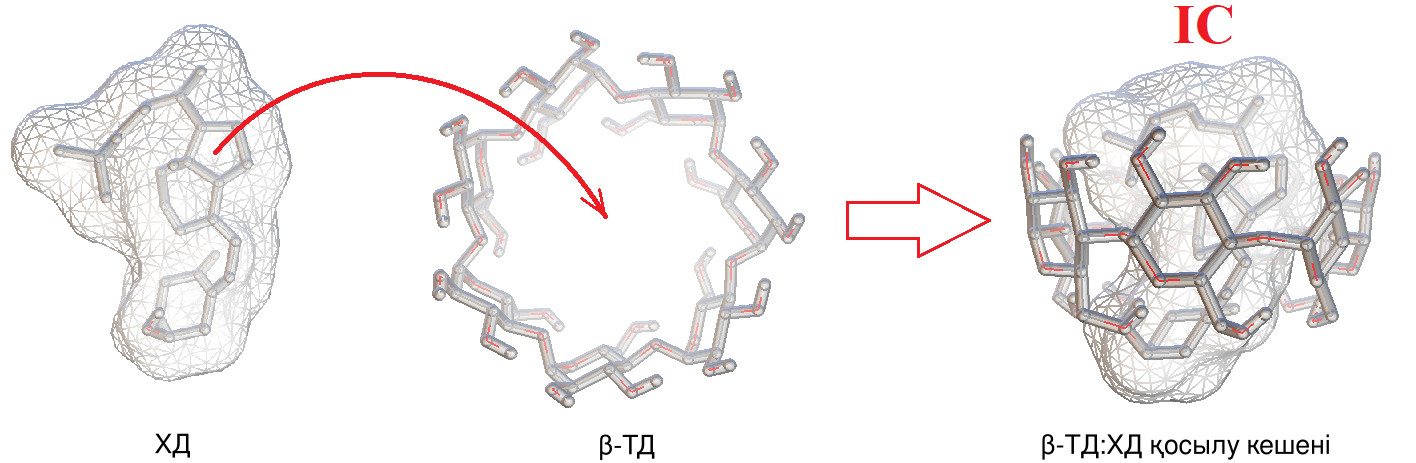
\includegraphics[width=0.8\textwidth]{image22}
\end{minipage}} \\
\midrule\noalign{}
\endhead
\bottomrule\noalign{}
\endlastfoot
ХД & β-ТД & β-ТД:ХД қосылу кешені \\
\end{longtable}

Сурет 1 - Холекальциферолдың β-ТД-мен қосылу кешенінің

қалыптасуының схемалық көрінісі

ХД тотықтырғыштардың әсерінен майлы қабық ішінде жақсы сақталады және
биожетімділігі жақсы болады {[}7{]}. Сондықтан ХД -ды β-ТД-мен кешенге
қосу табиғатын түсіну өте маңызды. Осы жұмыста біз β-ТД:ХД қосылу
кешенін микротолқынды әдіспен алдық {[}8{]}. Алынған кешен ИК-Фурье,
\textsuperscript{1}H және \textsuperscript{13}C ЯМР спектроскопиясы,
СEM, ДTГ әдістемелерімен зерттелді.

\textbf{Материалдар мен әдістемелер.} Жұмыста келесі реагенттер
қолданылды: олигосахарид β-тұйықдекстрин (β-ТД, Fluka фирмасынан сатып
алынған, 99,5\%), ХД (250 мкг (10.000 ХБ),
С\textsubscript{27}Н\textsubscript{44}О, (Олдрич компаниясы). ЯМР
\textsuperscript{1}Н, \textsuperscript{13}С барлық өлшемдері
DMSO-d\textsubscript{6} (Олдрич) ерітінділерінде жүргізілді, басқа
химиялық заттар реагенттер класының аналитикалық тазалығында болды.
(ХД)-нін тұйықдекстриндермен молекулалық докингтеу autodock 4.2.6,
MGLTools 1.5.7 {[}9{]} және AutoDock 4.2.6-да енгізілген ламарков
генетикалық алгоритмі (LGA) {[}10{]} бағдарламалары арқылы жүзеге
асырылды. Жартылай иілгіш қондыру әдісі қолданылды, онда рецептор қатты
зат ретінде қарастырылды, ал лиганд белгілі бір текше аймақта айналды
және қозғалыста болды. Байланыс энергиясы ретінде \emph{AutoDock}
электростатикалық, гидрофобты және сольвациялық әсерлерді, сондай-ақ
конфигурация энтропиясын қоса алғанда, еркін байланыс энергиясына
негізделген эмпирикалық бағалау функциясын пайдаланды. \emph{Autodock}
тәсілі торға негізделген молекулалық жақындық потенциалдарын қолдана
және энергияны жылдам бағалай отырып, Монте-Карлоның модельді үйлестіру
әдісін қолданады. Химиялық құрылымдар PubChem Substance and Compound
дерекқорынан алынды (pubchem.ncbi.nlm.nih.gov) {[}10{]}. Химиялық
құрылымның бірегей идентификаторлары ретінде 444041 (циклодекстрин),
5280795 (холекальциферол) алынды (сурет 2).

\begin{longtable}[]{@{}
  >{\raggedright\arraybackslash}p{(\columnwidth - 2\tabcolsep) * \real{0.4842}}
  >{\raggedright\arraybackslash}p{(\columnwidth - 2\tabcolsep) * \real{0.5158}}@{}}
\toprule\noalign{}
\begin{minipage}[b]{\linewidth}\raggedright
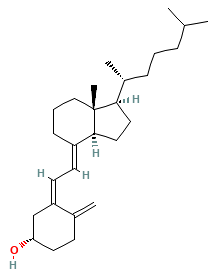
\includegraphics[width=0.8\textwidth]{image23}
\end{minipage} & \begin{minipage}[b]{\linewidth}\raggedright
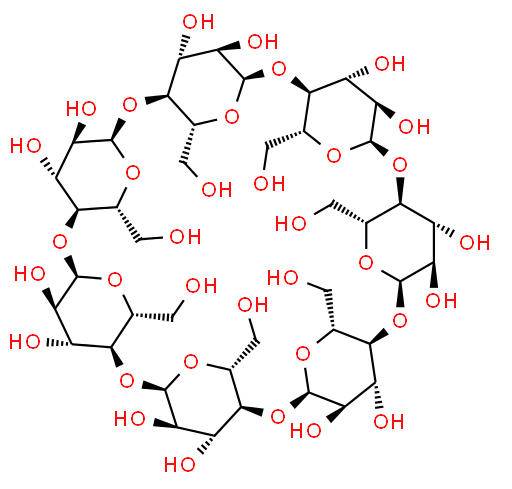
\includegraphics[width=0.8\textwidth]{image24}
\end{minipage} \\
\midrule\noalign{}
\endhead
\bottomrule\noalign{}
\endlastfoot
(a) Cholecalciferol (ДД\textsubscript{3}) & (b) β-ТД \\
\multicolumn{2}{@{}>{\raggedright\arraybackslash}p{(\columnwidth - 2\tabcolsep) * \real{1.0000} + 2\tabcolsep}@{}}{%
Сурет 2 -- Зерттеу нысандарының құрылымдарының формулалары} \\
\end{longtable}

(ХД)-дың β-ТД-мен қосылу кешендері (1:1; 1:2; 1:3) сулы-спиртті ортада
алынды. ХД мен β-ТД (ммоль ) қоспасы 600 секунд ішінде "Anton Paar
monowave 300" микротолқынды пеште 200 Вт сәулелену қуатымен 70°С
температурада әр 2 минуттік қадаммен өңделінді. Өңдеу аяқталғаннан кейін
еріткіштер алынып тасталды, ал өнімдер ацетонмен жуылып, эксикатор
ішінде CaCl\textsubscript{2} көмегімен тұрақты массаға дейін кептірілді.
β-ТД:ХД клатрат кешендерінің шығысы келесідей болды: 52,2 (1:1), 64.3
(1:2), 63,1 (1:3)\%. Алынған кешендер суда еритін ақ түсті кристалды
заттар болды, олар суда ақшыл түсті коллоидты ерітінді түзді. β-ТД:ХД
(2:1) кешенінің тазартылған суда ерігіштігі 0,20 мг±0,05/100 мл құрады.
β-ТД:ХД клатрат үлгілерінің бетінің морфологиясы LMN (Чехия) фирмасының
TesconMira3 сканерлеуші электронды микроскопының (СЭМ) көмегімен
зерттелді. ИҚ спектрлері 4000-400 см\textsuperscript{-1} диапазонында
Agilent Technologies (АҚШ) фирмасының CARY600 сериялы ИҚ-Фурье
спектрометрінде түсірілді. Алынған клатраттардың \textsuperscript{1}Н
және \textsuperscript{13}С ЯМР спектрлері DMSO-d6 еріткішін пайдаланып
Jnm-ECA Jeol400 спектрометрінде (сәйкесінше 399,78 және 100,53 МГц
жиіліктерде) тіркелді. β-ТД:ХД клатрат кешендерінің жылулық қасиеттері
labsys Evalution DTA/DTS дифференциалды сканерлеу калориметрінде
динамикалық режимде 30-500\textsuperscript{о}С температура диапазонында
азот атмосферасында 10 градус/мин қыздыру кезінде
Al\textsubscript{2}O\textsubscript{3} табақшасында жүргізілді,
температура диапазоны 30-800°С, үлгілердің қыздыру жылдамдығы 5-тен 20
к/мин дейін, үлгілердің массасы 12-16 мг болды, барлық есептеулер
Mathcad бағдарламасының көмегімен жүргізілді {[}11{]}.

\textbf{Нәтижелер және талқылау.} Молекулалық докинг әдісі тұрақты кешен
пайда болған кезде бір молекуланың екіншісіне қатысты артықшылықты
конфигурациясын дұрыс болжауға мүмкіндік береді. Сандық бағалау ретінде
рецептор молекуласы мен лиганд арасындағы байланыс энергиясы
қолданылады. Бастапқыда біз (β-ТД-дың β-ТД:ХД молекуласымен молекулалық
докингін олардың қосу кешендерінің 1:1 қатынасында байланысу энергиясын
анықтау үшін жасадық. (сурет 3).

\begin{longtable}[]{@{}
  >{\raggedright\arraybackslash}p{(\columnwidth - 4\tabcolsep) * \real{0.6467}}
  >{\raggedright\arraybackslash}p{(\columnwidth - 4\tabcolsep) * \real{0.1686}}
  >{\raggedright\arraybackslash}p{(\columnwidth - 4\tabcolsep) * \real{0.1846}}@{}}
\toprule\noalign{}
\multicolumn{2}{@{}>{\raggedright\arraybackslash}p{(\columnwidth - 4\tabcolsep) * \real{0.8154} + 2\tabcolsep}}{%
\begin{minipage}[b]{\linewidth}\raggedright
\begin{longtable}[]{@{}
  >{\raggedright\arraybackslash}p{(\columnwidth - 2\tabcolsep) * \real{0.5767}}
  >{\raggedright\arraybackslash}p{(\columnwidth - 2\tabcolsep) * \real{0.4233}}@{}}
\toprule\noalign{}
\begin{minipage}[b]{\linewidth}\raggedright
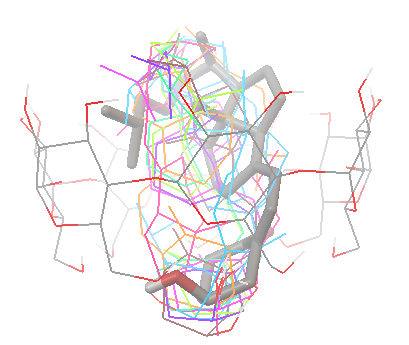
\includegraphics[width=0.8\textwidth]{image25}
\end{minipage} & \begin{minipage}[b]{\linewidth}\raggedright
\begin{longtable}[]{@{}
  >{\raggedright\arraybackslash}p{(\columnwidth - 2\tabcolsep) * \real{0.4738}}
  >{\raggedright\arraybackslash}p{(\columnwidth - 2\tabcolsep) * \real{0.5262}}@{}}
\toprule\noalign{}
\begin{minipage}[b]{\linewidth}\raggedright
Конформация нөмері
\end{minipage} & \begin{minipage}[b]{\linewidth}\raggedright
Байланыс энергиясы,

ккал/моль
\end{minipage} \\
\midrule\noalign{}
\endhead
\bottomrule\noalign{}
\endlastfoot
4 & -2.70 \\
7 & -0.17 \\
10 & +1.70 \\
6 & +4.22 \\
3 & +7.45 \\
8 & +17.43 \\
1 & +17.68 \\
5 & +27.93 \\
9 & +8.98 \\
2 & +23.00 \\
\end{longtable}
\end{minipage} \\
\midrule\noalign{}
\endhead
\bottomrule\noalign{}
\endlastfoot
\end{longtable}
\end{minipage}} & \begin{minipage}[b]{\linewidth}\raggedright
\end{minipage} \\
\midrule\noalign{}
\endhead
\bottomrule\noalign{}
\endlastfoot
\multicolumn{3}{@{}>{\raggedright\arraybackslash}p{(\columnwidth - 4\tabcolsep) * \real{1.0000} + 4\tabcolsep}@{}}{%
а) ХД-нің β-ТД-нің іш қуысындағы 10 түрлі мүмкін конформациясы} \\
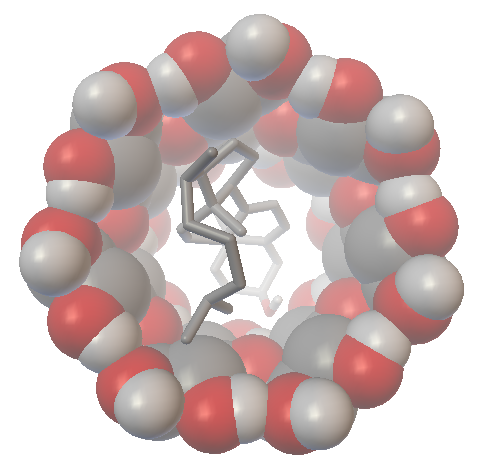
\includegraphics[width=0.8\textwidth]{image26} &
\multicolumn{2}{>{\raggedright\arraybackslash}p{(\columnwidth - 4\tabcolsep) * \real{0.3533} + 2\tabcolsep}@{}}{%
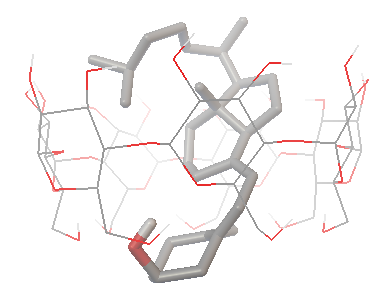
\includegraphics[width=0.8\textwidth]{image27}} \\
Жоғарыдан көрініс &
\multicolumn{2}{>{\raggedright\arraybackslash}p{(\columnwidth - 4\tabcolsep) * \real{0.3533} + 2\tabcolsep}@{}}{%
Бүйірден көрініс} \\
\multicolumn{3}{@{}>{\raggedright\arraybackslash}p{(\columnwidth - 4\tabcolsep) * \real{1.0000} + 4\tabcolsep}@{}}{%
(b) Ең жақсы байланысқан конформация (байланыс энергиясы = --2.7
ккал/моль)} \\
\multicolumn{3}{@{}>{\raggedright\arraybackslash}p{(\columnwidth - 4\tabcolsep) * \real{1.0000} + 4\tabcolsep}@{}}{%
Сурет 3 -- Холекальциферолдың β-ТД-мен докинг нәтижелері} \\
\end{longtable}

Докинг негізінде β-ТД мен ХД лигандысының 10 конформациясы алынды және
олардың байланысу энергиясы бағаланды. Сонымен қатар, ең жақсы
байланыстыруды 4-ші конформация көрсетті, оның байланысу энергиясы -2,7
ккал/моль болды. Байланыстыру энергиясының теріс мәні β-ТД-мен ХД
молекулалары арасында комплекс түзілуінінің мүмкіншілігін көрсетеді,
сонымен бірге өте төмен мән комплекс түзілу реакциясын жүргізудің арнайы
шарттарының қажеттілігі туралы айтуға мүмкіндік береді. ХД мен β-ТД
арасындағы байланыс энергиясының аз мөлшері назар аударады, сондықтан
AutoDock құралдарының көмегімен рецептор мен лиганд молекулалары
арасындағы сутегі байланыстарының болуын анықтау қызықты болып көрінді
(сурет 4).

\begin{longtable}[]{@{}
  >{\raggedright\arraybackslash}p{(\columnwidth - 0\tabcolsep) * \real{1.0000}}@{}}
\toprule\noalign{}
\begin{minipage}[b]{\linewidth}\raggedright
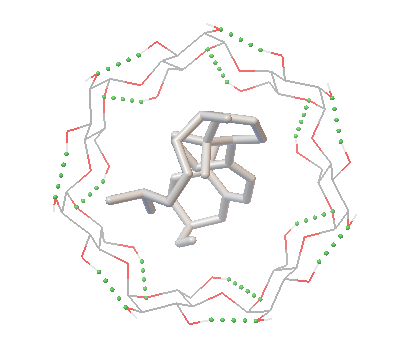
\includegraphics[width=0.8\textwidth]{image28}
\end{minipage} \\
\midrule\noalign{}
\endhead
\bottomrule\noalign{}
\endlastfoot
\end{longtable}

Сурет 4 -- ХД-дың β-ТД-мен кешендеріндегі

14 сутегі байланысының жүйесі

4-Суретте көрсетілген мәліметтерден бойынша β-ТД молекуласындағы ОН
топтары арасында 14 молекулаішілік сутегі байланысының жүйесі түзіледі.
Бұл жағдайда рецептор мен лиганд молекулалары арасында сутегі байланысы
байқалмайды. Рецептор мен лиганд арасында молекулааралық сутегі
байланысының болмауы олардың ТД-мен кешендерін молярлық 2:1 қатынасында
модельдеу болды. Ыңғайлы болу үшін β-ТД молекуласының кең жағы "бас"
("бас"), ал қарама-қарсы артқы жағы "құйрық" ("құйрық") деп белгіленді
(сурет. 5а). Бұл жағдайда екі β-ТД молекуласы арасында өзара
бағдарлаудың үш түрі болуы мүмкін: "бас-бас" (HH), бас-құйрық (HT) және
"құйрық-құйрық" (TT) (сурет 5б-г).

\begin{longtable}[]{@{}
  >{\raggedright\arraybackslash}p{(\columnwidth - 2\tabcolsep) * \real{0.4999}}
  >{\raggedright\arraybackslash}p{(\columnwidth - 2\tabcolsep) * \real{0.5001}}@{}}
\toprule\noalign{}
\begin{minipage}[b]{\linewidth}\raggedright
«Бас» («Head»)
\end{minipage} &
\multirow{3}{*}{\begin{minipage}[b]{\linewidth}\raggedright
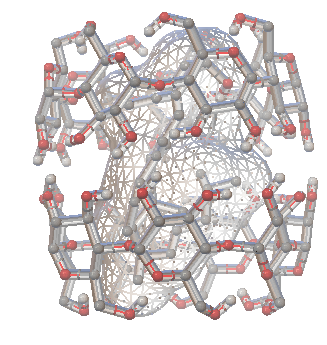
\includegraphics[width=0.8\textwidth]{image29}
\end{minipage}} \\
\begin{minipage}[b]{\linewidth}\raggedright
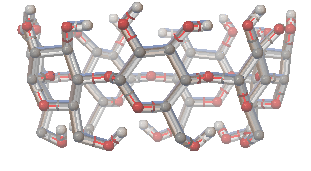
\includegraphics[width=0.8\textwidth]{image30}
\end{minipage} \\
\begin{minipage}[b]{\linewidth}\raggedright
«Құйрық» («Tail»)
\end{minipage} \\
\midrule\noalign{}
\endhead
\bottomrule\noalign{}
\endlastfoot
(a) β-ТД молекуласының бас және құйрығы & (б) кешеннің «бас басқа» (НН)
түрі

(байланыс энергиясы = -4.71 ккал/моль) \\
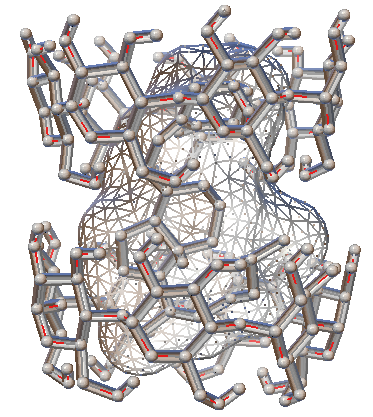
\includegraphics[width=0.8\textwidth]{image31} &
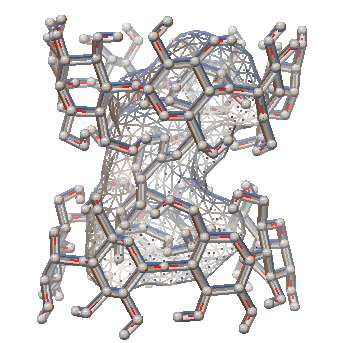
\includegraphics[width=0.8\textwidth]{image32} \\
(c) кешеннің «бас құйрыққа» түрі (HT),

(байланыс энергиясы = -7.32 ккал/моль) & (д) кешеннің «құйрық құйрыққа»
түрі (TT),

(байланыс энергиясы = +3.85 ккал/моль) \\
\end{longtable}

Сурет 5 -- β-ТД молекуласы (а) және оның ХД-мен кешендерінің үш түрі
(2:1)

5-Суретте көрініп тұрғандай, 1:1 (-2,7 ккал/моль) комплексімен
салыстырғанда, "бас-бас" (HH) және "бас-құйрық" (HT) кешендерінің екі
түрі тиімдірек байланыстыруды (тиісінше -4,71 және -7,32 ккал/моль)
көрсетеді. "Құйрық-құйрық" типті кешен оң байланыс энергиясын көрсетеді,
бұл осы типтегі кешеннің түзілу мүмкіншілігінің аз екенін көрсетеді. Бұл
жағдайда "бас-құйрық" (с) кешені максималды байланыс энергиясын
көрсетеді, бұл мұндай кешеннің үлкен тұрақтылығын көрсетеді {[}11,12{]}.

Қарастырылып отырған физикалық жағдайға байланысты зерттелетін
объектілерді сипаттау үшін әртүрлі әдістерді қолдану модельдердің
сенімділігі тұрғысынан жақсы нәтиже береді. 6-Суретте β-ТД-нің, β-ТД+ ХД
физикалық қоспасының және β-ТД:ХД (2:1) қосылу кешенінің микросуреттері
көрсетілген. Клатрат түзілуіндегі кристалл беті морфологиясының өзгеруі
қосу кешенінің пайда болуының күшті дәлелі болып табылады {[}13,14{]}.

\begin{longtable}[]{@{}
  >{\raggedright\arraybackslash}p{(\columnwidth - 4\tabcolsep) * \real{0.3360}}
  >{\raggedright\arraybackslash}p{(\columnwidth - 4\tabcolsep) * \real{0.3360}}
  >{\raggedright\arraybackslash}p{(\columnwidth - 4\tabcolsep) * \real{0.3281}}@{}}
\toprule\noalign{}
\begin{minipage}[b]{\linewidth}\raggedright
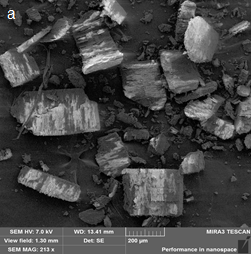
\includegraphics[width=0.8\textwidth]{image33}
\end{minipage} & \begin{minipage}[b]{\linewidth}\raggedright
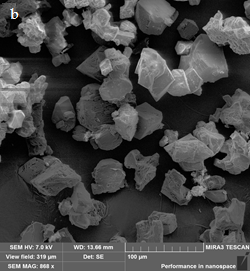
\includegraphics[width=0.8\textwidth]{image34}
\end{minipage} & \begin{minipage}[b]{\linewidth}\raggedright
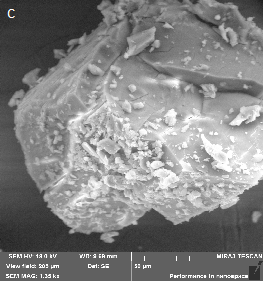
\includegraphics[width=0.8\textwidth]{image35}
\end{minipage} \\
\midrule\noalign{}
\endhead
\bottomrule\noalign{}
\endlastfoot
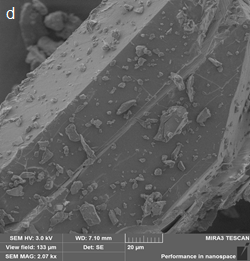
\includegraphics[width=0.8\textwidth]{image36} &
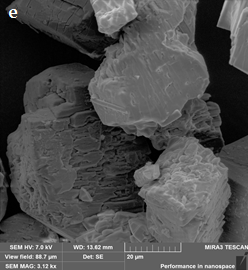
\includegraphics[width=0.8\textwidth]{image37} &
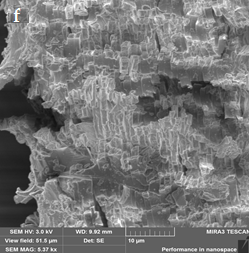
\includegraphics[width=0.8\textwidth]{image38} \\
\end{longtable}

Сурет 6 -- β-ТД (а, b), β-ТД +ХД-ның физикалық қоспасының және β-ТД:ХД
(2:1) (e, f) клатратының әр түрлі үлкейтудегі электронды микросуреттері

ИҚ спектрлерде (сурет 7) О-Н байланысының валенттік тербелістері 3398
(β-ТД (a), 3564 (ТД\textsubscript{3} (b) және 3368
см\textsuperscript{--1} (β-ТД:ХД (c) аймақтарында кең жолақ түрінде
анықталады. Сондай-ақ, CH және CН\textsubscript{2} топтарындағы CH
байланыстарының валенттік тербелістеріне тән сіңіру жолағы 2924
см\textsuperscript{-1}-де бар {[}15{]}. β-ТД:ХД кешенінің ИҚ
спектрлерінде C=C, ОН және ВД\textsubscript{3}-ның басқа топтарының
сіңіру жолақтары көрінбейді. Бұл осы топтардың толқын ұзындығының бірдей
диапазонында өте кең және қарқынды β-ТД жолақтарының көлеңкесінен
көрінбеуі мүмкін. 1643 см\textsuperscript{-1} аймағында β-ТД:ХД
кешенінің С=О тобының қарқынды жолағы бар. Қосылу кешендерінің түзілуін
растаудың ақпараттық әдістерінің бірі-спектроскопияның
\textsuperscript{1}Н ЯМР әдісі {[}16{]}. Бұл әдіс ТД молекуласының ішкі
қуысында бағытталған β-ТД H-3 және H-5 протондарының тербелмелі
спектрлеріндегі олардың химиялық ыдысуын айқын байқауға мүмкіндік
береді. Клатраттың \textsuperscript{1}Н ЯМР спектрінде барлық алты β-ТД
протондары күшті өрісте айқын химиялық ыдысуды көрсетті. β-ТД:ХД (2:1)
кешенінің \textsuperscript{1}H ЯМР спектрлеріндегі Δδ химиялық ыдысу
мәндеріндегі ең үлкен айырмашылық H-3 (-0.112) және H-5 (-0.108)
сфераішілік протондарына тән. Бұл деректер циклодекстриннің гидрофобты
қуысында ішкі (инклюзивті) кешен пайда болады деген қорытынды жасауға
мүмкіндік береді.

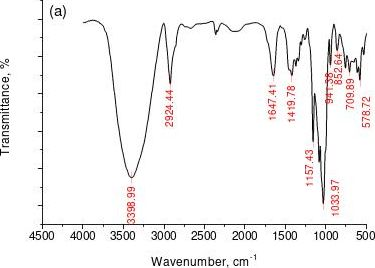
\includegraphics[width=0.8\textwidth]{image39}
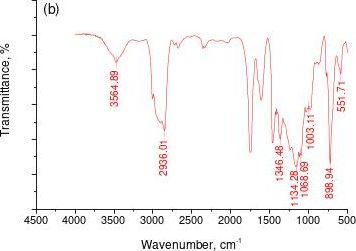
\includegraphics[width=0.8\textwidth]{image40}

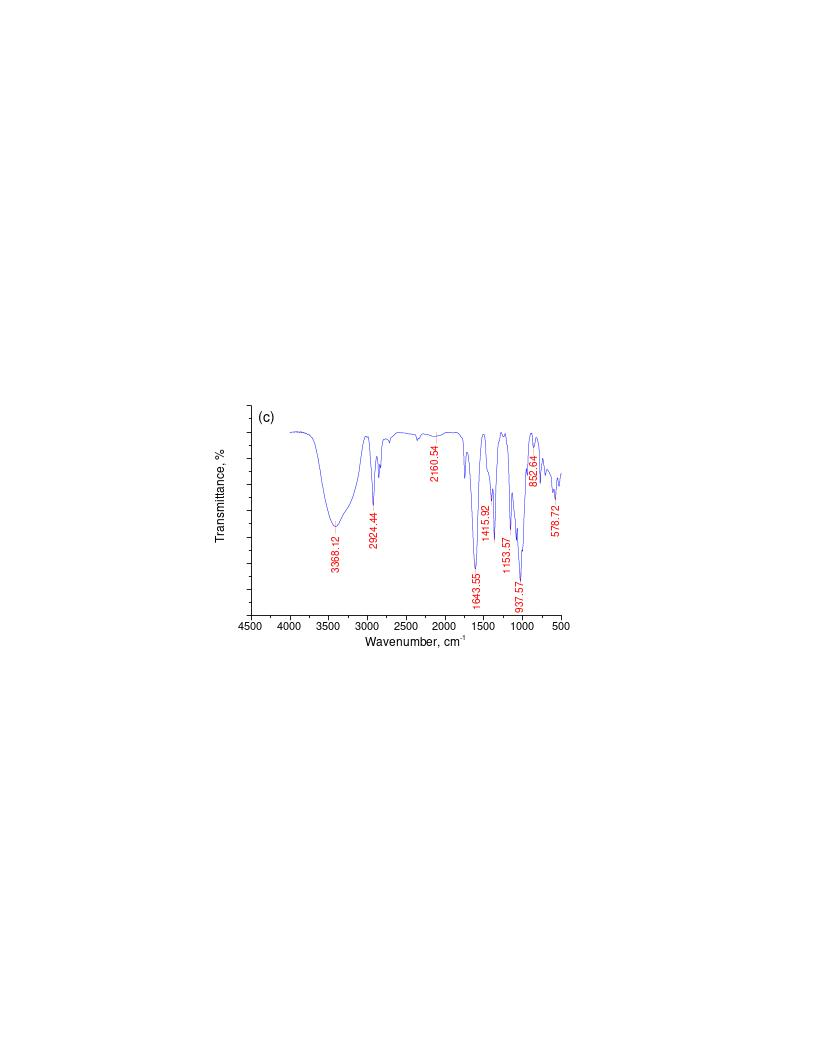
\includegraphics[width=0.8\textwidth]{image41}

Сурет 7 -- β-ТД (a), ХД (b) және β-ТД:ХД (2:1) клатратының ИК спектрлері

β-ТД:ДД\textsubscript{3} кешендерінің термиялық қасиеттерін талдау
термогравиметриялық талдау әдісімен жүргізілді {[}17{]}. Суретте 8а,b
β-ТД мен оның β-ТД:ХД (2:1) клатратының ТГ мен ДТГ термограммалары
көрсетілген (қыздыру жылдамдығы 10 градус/мин).

β-ТД және оның β-ТД:ХД клатратының термоаналитикалық ыдырау
көрсеткіштері (2:1) TГ/ДTГ сызықтық қисықтарымен ұсынылған (сурет 8a,b).
Термогравиметриялық β-ТД қисықтары мен β-ТД:ХД клатратын салыстыру
арқылы (сурет 8a,b), β-ТД:ХД клатраты үшін
\textasciitilde124\textsuperscript{о}\textasciitilde{} \textasciitilde{}
235\textsuperscript{о}С температура диапазонында үлгі массасының
қарқынды төмендеуі байқалатынын көреміз (\textasciitilde77,27 \%). TG
қисығының бұл бөлімі \textasciitilde235\textsuperscript{о}С
температурада ДТГ қисығындағы массаның жоғалу жылдамдығының максималды
өзгеруіне сәйкес келеді (сурет 8b).

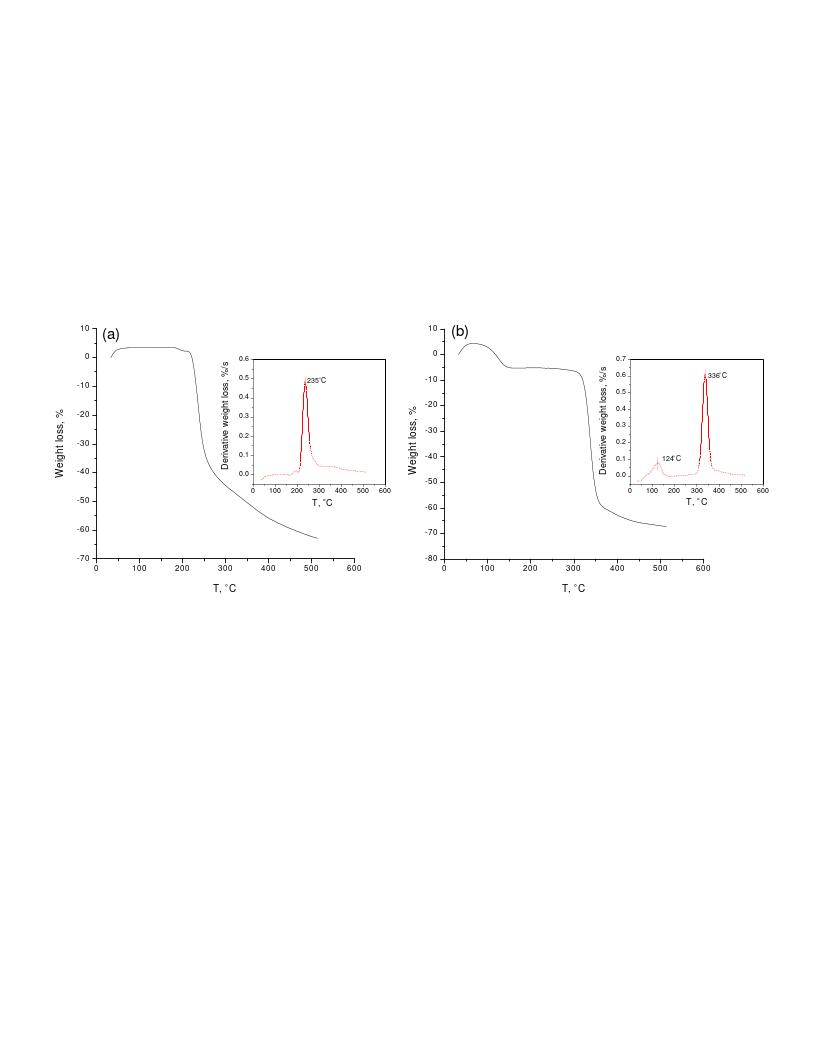
\includegraphics[width=0.8\textwidth]{image42}

Сурет 8 -- β-ТД:ХД кешенінің азотты ортада 10 градус/мин тұрақты қыздыру
жылдамдығы жағдайында алынған TГ/ДТГ қисықтары: а) физикалық қоспа; b)
β-ТД:ХД (2:1)

β-ТД:ХД клатраттарындағы массаның төмен температурада
(\textasciitilde1240с) жоғалуы ылғалдың жойылуымен байланысты, бұл ДТГ
деректерімен де расталады (сурет 8b). Алынған β-ТД:ХД кешендерінде,
бастапқы β-ТД сияқты, байланысқан су болды. Алынған мәліметтер негізінде
β-ТД:ХД (2:1) клатратының термиялық ыдырауының кинетикалық параметрлері
есептелді (кесте 3) {[}13{]}. β-ЦД мен β-ТД:ХД (2:1) клатратының
термиялық тұрақтылығын салыстыру үшін ыдырау реакциясының активтену
энергиялары анықталды. β-ЦД және β-ТД:ХД (2:1) кешендерінің термиялық
ыдырауының есептеулерін салыстыра отырып β-ТД мен оның клатратының (2:1)
активтену энергиялары бірдей конверсия дәрежелерінде (\emph{α}) әр түрлі
болады деп айтуға болады (кесте).

Кесте -- β-ТД мен β-ТД:ХД (2:1) клатратының азотты ортада активтену
энергиясының мәндері

\begin{longtable}[]{@{}
  >{\raggedright\arraybackslash}p{(\columnwidth - 4\tabcolsep) * \real{0.3037}}
  >{\raggedright\arraybackslash}p{(\columnwidth - 4\tabcolsep) * \real{0.3750}}
  >{\raggedright\arraybackslash}p{(\columnwidth - 4\tabcolsep) * \real{0.3212}}@{}}
\toprule\noalign{}
\begin{minipage}[b]{\linewidth}\raggedright
Үлгі
\end{minipage} & \begin{minipage}[b]{\linewidth}\raggedright
E\textsubscript{a}, кДж/моль
\end{minipage} & \begin{minipage}[b]{\linewidth}\raggedright
A, с\textsuperscript{-1}
\end{minipage} \\
\midrule\noalign{}
\endhead
\bottomrule\noalign{}
\endlastfoot
β-ТД & 164.58 & 1.10·10\textsuperscript{17} \\
β-ТД:ХД (2:1) & 103.50 & 8.96·10\textsuperscript{10} \\
\end{longtable}

\textbf{Қорытынды.} Жүргізілген зерттеулердің нәтижелері
холекальциферолдың (ХД) β-олигоқантпен (β-ТД) суда еритінді қосылу
кешенін алу мүмкіндігін көрсетті, оны тағамды дәрумендеу үшін қолдануға
болады. \emph{In silico} зерттеу жағдайында молекулалық модельдеу және
докинг әдістерін қолдану ХД-нің β-ТД-мен қосылу кешендерінің түзілу
механизмдерінің жалпы көрінісін жасауға мүмкіндік берді. Модельдер
жартылай иілгіш қондыру әдісін қолданды, онда рецептор қатты зат ретінде
қарастырылды, ал лиганд белгілі бір текше аймақта айналды және қозғалыс
жағдайында болды. Зерттелетін объектілерді сипаттау үшін қарастырылып
отырған физикалық жағдайға байланысты әртүрлі физиохимиялық әдістерді
қолдану модельдердің сенімділігі тұрғысынан жақсы нәтиже береді. Майлы
ортада еритін ХД дәруменінің β-олигоқантпен микротолқынды белсендіру
жағдайында сулы-спиртті ортада әрекеттесуі оның суда еритін
супрамолекулярлы қосылу кешенінің түзілуіне әкелді. ХД-ді клатратты
кешенге қаптау дәруменнің майлы ерітіндісінің агрегаттық күйінің
өзгеруіне әкелді. Синтезделген β-ТД:ХД кешені "қонақ-қожайын"
қосылыстарына жатады және жақсы ерігіштікке ие. Клатрат кешенінің
түзілуіндегі шешуші мәселе арнайы байланыс емес (гидрофобты,
дисперсиялық және ван-дер-Ваальс) өзара әрекеттесулерге жатады.

\emph{Алғыс, мүдделер қақтығысы (қаржыландыру\textbf{)-} Қаржыландыру,
биологиялық белсенді заттарды инкапсуляциялау әдістерін әзірлеу
жөніндегі ғылыми зерттеуді Қазақстан Республикасы Білім және ғылым
министрлігінің Ғылым комитеті қолдады (PTF № BR10965230, 2021-2023).}

\textbf{Әдебиеттер}

1. Mauryaa V.K., Bashirb K., Aggarwala M. Vitamin D microencapsulation
and fortification: Trends and technologies // Journal of Steroid
Biochemistry and Molecular Biology. --2020. --Vol.196. --No.105489.

2. Brett N.R., Lavery P., Vanstone C.A., Maguire J.L., Rauch F., Weiler
H.A. Dietary vitamin D dose-response in healthy children 2 and 8 y of
age: a 12-wk randomized controlled trial using fortified foods // Am. J.
Clin. Nutr. --2016. -- Vol. 103. --P.144-152.

3. Abu el Maaty M., Almouhanna F., Wölfl S. Expression of TXNIP in
cancer cells and regulation by 1, 25 (OH) 2D\textsubscript{3}: is it
really the vitamin D\textsubscript{3} upregulated protein // Int. J.
Mol. Sci. --2018. --Vol.19. -- Issue No 3. --P.796-803.

4. Atteritano M., Mirarchi L., Venanzi-Rullo E., Santoro D., Iaria C.,
Catalano A., Lasco A., Arcoraci V., Lo Gullo A., Bitto A. Vitamin D
status and the relationship with bone fragility fractures in
HIV-infected patients: a case control study // Int. J. Mol. Sci. --2018.
--Vol.19. --P.119.

5. Legarth C., Grimm D., Wehland M., Bauer J., Krüger M. The impact of
vitamin D in the treatment of essential hypertension. Int. J. Mol. Sci.
--2018. --Vol.19. --Issue No 2. --P. 455.

6. Wierzbicka J., Binek A., Ahrends T., Nowacka J.D., Szydłowska A.,
Tuckey R. Differential antitumor effects of vitamin D analogues on
colorectal carcinoma in culture // Int. J. Oncol. --2015. --Vol. 47.
--P.1084-1096.

7. Larsen, K.L. Large cyclodextrins //J. Incl. Phenom. Mycrocycl. Chem.
--2002, -- Vol.43(1), --Р.1-13.

8. Zhao D., Liao K., Ma X., Yan X. Study of the supramolecular inclusion
of~\emph{β}-cyclodextrin with andrographolide //
\href{https://link.springer.com/journal/10847}{Journal of Inclusion
Phenomena and Macrocyclic Chemistry}. --2002. --Vol.43. --259-264.

9 Morris G. M., Huey R., Lindstrom W., Sanner M. F., Belew R. K.,
Goodsell D.S. and Olson A.J. ``Autodock4 and AutoDockTools4: automated
docking with selective receptor flexibility // J. Computational
Chemistry. --2009. --Vol.16. --P.2785-2791.

10. Fuhrmann J., Rurainski A., Lenhof H. P., Neumann D. A new Lamarckian
genetic algorithm for flexible ligand-receptor docking // Journal of
computational chemistry. --2010. --Vol. 31. -- Issue No.9.
--P.1911--1918.

11. Kim S., Chen J., Cheng T., Gindulyte A., He J., He S., Li Q.,
Shoemaker B. A., Thiessen P.A., Yu B., Zaslavsky L., Zhang J.,
\emph{Bolton E.E.} PubChem in 2021: new data content and improved web
interfaces \emph{//~}Nucleic Acids Res.~ --2019. --Vol.49(D1).
--P.D1388--D1395.

12. Bulani V.D., Kothavade P.S., Kundaikar H.S., Gawali N.B., Chowdhury
A.A., Degani M.S., Juvekar A.R. Inclusion complex of ellagic acid with
β-cyclodextrin: Characterization and in vitro anti-inflammatory
evaluation //~J. Mol. Struct\emph{.}~--2016. --Vol.1105. --P.308-315.

13. Bakirova R., Nukhuly A., Iskineyeva A., Fazylov S., Burkeev M.,
Mustafaeva A., Minaeva E., Sarsenbekova A. Obtaining and Investigation
of the beta-Cyclodextrin Inclution Complex with Vitamin
D\textsubscript{3} Oil // Scientifica. --2020. --Vol.1-8. ~-- ID
6148939. DOI: 10.1155/2020/6148939.

14. Liu Y., Zhang H. ``Study of VD\textsubscript{3}-β-Cyclodextrin
Inclusion Complex //Journal of Geoscience and Environment
Protection\emph{.} --2016. --Vol.4. --Issue 4. --P.163-167

15. Zou A., Zhao X., Handge U.A., Garamus V.M., Willumeit-Römer R., Yin
P. Folate receptor targeted bufalin/\emph{β}-cyclodextrin supramolecular
inclusion complex for enhanced solubility and anti-tumor efficiency of
bufalin //Mater. Sci. Eng. --2017. --Vol.78. --P.609-618.

16. Dodziuk H., Koźmiński W., Ejchart A. NMR studies of chiral
recognition by cyclodextrines //Chirality\emph{.} --2004. -- Vol.16.
--Issue No.2. --P.90-105.

\textbf{References}

1. Mauryaa V.K., Bashirb K., Aggarwala M. Vitamin D microencapsulation
and fortification: Trends and technologies // Journal of Steroid
Biochemistry and Molecular Biology. --2020. --Vol.196. --No.105489.

2. Brett N.R., Lavery P., Vanstone C.A., Maguire J.L., Rauch F., Weiler
H.A. Dietary vitamin D dose-response in healthy children 2 and 8 y of
age: a 12-wk randomized controlled trial using fortified foods // Am. J.
Clin. Nutr. --2016. -- Vol. 103. --P.144-152.

3. Abu el Maaty M., Almouhanna F., Wölfl S. Expression of TXNIP in
cancer cells and regulation by 1, 25 (OH) 2D\textsubscript{3}: is it
really the vitamin D\textsubscript{3} upregulated protein // Int. J.
Mol. Sci. --2018. --Vol.19. -- Issue No 3. --P.796-803.

4. Atteritano M., Mirarchi L., Venanzi-Rullo E., Santoro D., Iaria C.,
Catalano A., Lasco A., Arcoraci V., Lo Gullo A., Bitto A. Vitamin D
status and the relationship with bone fragility fractures in
HIV-infected patients: a case control study // Int. J. Mol. Sci. --2018.
--Vol.19. --P.119.

5. Legarth C., Grimm D., Wehland M., Bauer J., Krüger M. The impact of
vitamin D in the treatment of essential hypertension. Int. J. Mol. Sci.
--2018. --Vol.19. --Issue No 2. --P. 455.

6. Wierzbicka J., Binek A., Ahrends T., Nowacka J.D., Szydłowska A.,
Tuckey R. Differential antitumor effects of vitamin D analogues on
colorectal carcinoma in culture // Int. J. Oncol. --2015. --Vol. 47.
--P.1084-1096.

7. Larsen, K.L. Large cyclodextrins //J. Incl. Phenom. Mycrocycl. Chem.
--2002, -- Vol.43(1), --Р.1-13.

8. Zhao D., Liao K., Ma X., Yan X. Study of the supramolecular inclusion
of~\emph{β}-cyclodextrin with andrographolide //
\href{https://link.springer.com/journal/10847}{Journal of Inclusion
Phenomena and Macrocyclic Chemistry}. --2002. --Vol.43. --259-264.

9 Morris G. M., Huey R., Lindstrom W., Sanner M. F., Belew R. K.,
Goodsell D.S. and Olson A.J. ``Autodock4 and AutoDockTools4: automated
docking with selective receptor flexibility // J. Computational
Chemistry. --2009. --Vol.16. --P.2785-2791.

10. Fuhrmann J., Rurainski A., Lenhof H. P., Neumann D. A new Lamarckian
genetic algorithm for flexible ligand-receptor docking // Journal of
computational chemistry. --2010. --Vol. 31. -- Issue No.9.
--P.1911--1918.

11. Kim S., Chen J., Cheng T., Gindulyte A., He J., He S., Li Q.,
Shoemaker B. A., Thiessen P.A., Yu B., Zaslavsky L., Zhang J.,
\emph{Bolton E.E.} PubChem in 2021: new data content and improved web
interfaces \emph{//~}Nucleic Acids Res.~ --2019. --Vol.49(D1).
--P.D1388--D1395.

12. Bulani V.D., Kothavade P.S., Kundaikar H.S., Gawali N.B., Chowdhury
A.A., Degani M.S., Juvekar A.R. Inclusion complex of ellagic acid with
β-cyclodextrin: Characterization and in vitro anti-inflammatory
evaluation //~J. Mol. Struct\emph{.}~--2016. --Vol.1105. --P.308-315.

13. Bakirova R., Nukhuly A., Iskineyeva A., Fazylov S., Burkeev M.,
Mustafaeva A., Minaeva E., Sarsenbekova A. Obtaining and Investigation
of the beta-Cyclodextrin Inclution Complex with Vitamin
D\textsubscript{3} Oil // Scientifica. --2020. --Vol.1-8. ~-- ID
6148939. DOI: 10.1155/2020/6148939.

14. Liu Y., Zhang H. ``Study of VD\textsubscript{3}-β-Cyclodextrin
Inclusion Complex //Journal of Geoscience and Environment
Protection\emph{.} --2016. --Vol.4. --Issue 4. --P.163-167

15. Zou A., Zhao X., Handge U.A., Garamus V.M., Willumeit-Römer R., Yin
P. Folate receptor targeted bufalin/\emph{β}-cyclodextrin supramolecular
inclusion complex for enhanced solubility and anti-tumor efficiency of
bufalin //Mater. Sci. Eng. --2017. --Vol.78. --P.609-618.

16. Dodziuk H., Koźmiński W., Ejchart A. NMR studies of chiral
recognition by cyclodextrines //Chirality\emph{.} --2004. -- Vol.16.
--Issue No.2. --P.90-105.

\emph{\textbf{Information about authors:}}

Serik Fazylov -- Academician of the National Academy of the Republic of
Kazakhstan, Doctor of Chemical Sciences, Full Professor, Institute of
Organic Synthesis and Coal Chemistry, Alikhanov str. 1, 100008,
Karaganda, Kazakhstan; е-mail:
\ul{\href{mailto:iosu8990@mail.ru}{\nolinkurl{iosu8990@mail.ru}};}
\ul{\url{https://orcid.org/0000-0002-4240-6450}.} \emph{(Corresponding
author)}

Oralgazy Nurkenov -- Doctor of Chemical Sciences, Full Professor,
Institute of Organic Synthesis and Coal Chemistry, Alikhanov str. 1,
100008, Karaganda, Kazakhstan; е-mail:
\ul{\href{mailto:nurkenov_oral@mail.ru}{\nolinkurl{nurkenov\_oral@mail.ru}};}
\ul{\url{https://orcid.org/0000-0003-1878-2787}.}

Ainara Iskineyeva - PhD student of Saken Seifullin Kazakh Agrotechnical
University, Nur-Sultan, Kazakhstan, e-mail: iskeneeva\_aynara@mail.ru,
https://orcid.org/0000-0002-1705-6372.

Ayaulim Mustafayeva - Candidate of Thechnical Sciences, Saken Seifullin
Kazakh Agrotechnical University, Nur-Sultan, Kazakhstan, e-mail:
ayaulym.mustafa@mail.ru,
\href{https://orcid.org/0000-0003-0693-6427}{\ul{https://orcid.org/0000-0003-0693-6427}}.

Irina Pustolaikina -- Candidate of Chemical Sciences, Assoc. Professor,
Karagandy University of the name of academician E.A.~Buketov,
Universitetskaya street, 28, 100024, Karaganda, Kazakhstan; e-mail:
\href{mailto:ipustolaikina@gmail.com}{\ul{ipustolaikina@gmail.com}},
\ul{\url{https://orcid.org/0000-0001-6319-666X}.}

Akmaral Sarsenbekova - PhD, Assoc. Professor,, Karagandy University of
the name of academician E.A.~Buketov, Universitetskaya street, 28,
100024, Karaganda, Kazakhstan; e-mail:
\href{mailto:chem_akmaral@mail.ru}{\ul{chem\_akmaral@mail.ru}},
\ul{\url{https://orcid.org/0000-0002-8951-3616}.}

Aleksandr Sviderskiy -- Doctor of Chemical Sciences, Full Professor,
Innovativ Eurasian University, Lomova Str. 45, 140000, Pavlodar,
Kazakhstan; e-mail:
\href{mailto:katsostud@mail.ru}{\ul{katsostud@mail.ru}},
https://orcid.org/0000-0001-7277-5882.

МРНТИ 61.13.17; 31.15.27

\textbf{КИНЕТИКА ТЕРМИЧЕСКОЙ ДЕСТРУКЦИИ УГЛЯ МЕСТОРОЖДЕНИЯ КИЯКТЫ}

\textbf{Н.У. Нургалиев\textsuperscript{*},} \textbf{А.Х.Такирова, А.Ж.
Хамит, Э.Б. Жунусова, А.А. Ахаева}

Казахский университет технологии и бизнеса, г. Астана, Казахстан,

e-mail:
\href{mailto:nurgaliev_nao@mail.ru}{\nolinkurl{nurgaliev\_nao@mail.ru}}

В статье проведено исследование кинетики термической деструкции угля с
использованием метода термогравиметрического анализа. Нагрев образцов
угля проводили в керамических тиглях в интервале температур 25-900 °С
при разных скоростях нагрева (3-15 град/мин) в средах азота и кислорода.
В качестве объекта исследования выбран уголь месторождения Киякты
(Казахстан). На основе построенных дифференциальных термических кривых
DTG (зависимость скорости изменения массы образца от времени) при разных
скоростях нагрева рассчитаны кинетические параметры термодеструкции
угля, с использованием уравнений неизотермической формальной кинетики.
Изучено влияние скорости и температуры нагрева угля на кинетические
параметры процесса термической деструкции органической массы угля (ОМУ).
Выявлены основные стадии разложения ОМУ. Установлено, что скорость
нагрева образцов угля заметно влияет на значения температуры и скорости
процесса, соответствующие максимумам основного разложения на
дифференциальных кривых DTG.

\textbf{Ключевые слова:} термогравиметрический анализ, уголь,
термическая деструкция, кривые DTG, кинетические параметры, стадии
разложения, скорость нагрева.

\textbf{ҚИЯҚТЫ КЕН ОРЫНЫ КӨМІРНІҢ ТЕРМИЯЛЫҚ ДЕСТРУКЦИЯСЫНЫҢ КИНЕТИКАСЫ}

\textbf{Н.У. Нургалиев\textsuperscript{*}, А.Х.} \textbf{Такирова, А.Ж.
Хамит, Э.Б. Жунусова, А.А.Ахаева}

Қазақ технология және бизнес университеті, Астана, Қазақстан

e-mail:
\href{mailto:nurgaliev_nao@mail.ru}{\nolinkurl{nurgaliev\_nao@mail.ru}}

Мақалада термогравиметриялық анализ әдісін қолдану арқылы көмірдің
термиялық деградациясының кинетикасы зерттеу жасалған. Көмір үлгілері
қыш тигельдерде 25--900°C температура диапазонында азот пен оттегі
орталарында әртүрлі қыздыру жылдамдықтарында (3--15 град/мин)
қыздырылды. Зерттеу нысаны ретінде Қияқты кен орнының көмірі (Қазақстан)
таңдалды. Құрылған дифференциалдық қисықтар негізінде DTG (үлгі
массасының өзгеру жылдамдығының уақытқа тәуелділігі) әртүрлі қыздыру
жылдамдықтарында көмірдің термиялық деструкциясының кинетикалық
параметрлері изотермиялық емес формалды кинетика теңдеулері арқылы
есептелді. Көмірдің органикалық массасының (КОМ) термиялық бұзылу
процесінің кинетикалық параметрлеріне көмірді қыздыру жылдамдығы мен
температурасының әсері зерттелді.

КОМ ыдырауының негізгі кезеңдері анықталды. Көмір үлгілерін қыздыру
жылдамдығы DTG дифференциалды қисықтары бойынша негізгі ыдырау
максимумдарына сәйкес келетін температура мен технологиялық процестің
жылдамдығына айтарлықтай әсер ететіні анықталды.

\textbf{Түйінді сөздер:} термогравиметриялық талдау, көмір, термиялық
деградация, DTG қисықтары, кинетикалық параметрлер, ыдырау кезеңдері,
қыздыру жылдамдығы.

\textbf{KINETICS OF THERMAL DESTRUCTION OF COAL FROM THE KIYAKTY
DEPOSIT}

\textbf{N.U. Nurgaliyev\textsuperscript{*}, A.K. Takirova, A.Z. Khamit,
E.B. Zhunussova, A.A.Akhaeva}

Kazakh University of Technology and Business, Astana, Kazakhstan,

e-mail:
\href{mailto:nurgaliev_nao@mail.ru}{\nolinkurl{nurgaliev\_nao@mail.ru}}

The article studies the kinetics of thermal degradation of coal using
the method of thermogravimetric analysis. Coal samples were heated in
ceramic crucibles in the temperature range of 25--900°C at different
heating rates (3--15 deg/min) in nitrogen and oxygen media. Coal from
the Kiyakty deposit (Kazakhstan) was chosen as the object of study.
Based on the constructed differential thermal curves DTG (dependence of
the sample mass change rate on time) at different heating rates, the
kinetic parameters of thermal degradation of coal were calculated using
the equations of non-isothermal formal kinetics. The influence of the
rate and temperature of coal heating on the kinetic parameters of the
process of thermal destruction of the organic mass of coal (OMC) has
been studied. The main stages of WMD decomposition are revealed. It has
been found that the heating rate of coal samples significantly affects
the temperature and process rate corresponding to the main decomposition
maxima on the differential DTG curves.

\textbf{Keywords:} thermogravimetric analysis, coal, thermal
degradation, DTG curves, kinetic parameters, decomposition stages,
heating rate.

\textbf{Введение.} Для повышения экологичности и эффективности
использования твердого топлива предложены различные решения, от
газификации до оптимизации эксплуатационных параметров с применением
математического моделирования процессов деструкции. Это объясняет
повышенный интерес к исследованию кинетики процессов деструкции твердых
топлив в последнее время {[}1-4{]}. Одним из наиболее известных методов
термического анализа является метод термогравиметрического анализа
(ТГА), позволяющий исследовать основные параметры окисления твердого
топлива, в т.ч. определять кинетические параметры исследуемого процесса.

Достаточно широко распространены работы с применением ТГА {[}5-9{]},
посвященные определению констант формальной кинетики процессов конверсии
угля. Подобные работы основаны на интерпретации уравнения Аррениуса и
предположении о том, что скорость уменьшения массы твердого топлива
зависит только от температуры и степени конверсии {[}10{]}. Целью данных
работ является нахождении параметров \emph{E} и \emph{A}, называемых
энергией активации и предэкспонентой соответственно, а также
кинетической функции f(α). Вместе, эти три величины называют
кинетическим триплетом {[}11{]}.

При рассмотрении термической деструкции классическая кинетика отдельно
описывает влияние концентрации и температуры реагирующих веществ на
скорость процесса, без учета изменения концентрации в зависимости от
температуры. В неизотермической кинетике нет этого недостатка {[}12{]}.
С помощью неизотермических методов можно за относительно небольшой
промежуток времени получить важную информацию о характере протекания
процесса термодеструкции в широком температурном интервале.

Цель настоящей работы ‒ исследование зависимости скорости и температуры
нагрева угля от кинетических параметров термической деструкции ОМУ с
использованием метода ТГА. В качестве объекта исследования выбран уголь
месторождения Киякты (Казахстан). Задачами исследования является
определение основных стадий разложения ОМУ, изучение влияния скорости и
температуры нагрева угля на кинетику термодеструкции.

\textbf{Материалы и методы.} Эксперименты по исследованию кинетики
термического разложения угля месторождения Киякты проводили на
термогравиметрическом анализаторе TGA4000 при разных скоростях нагрева в
пределах 3-15 град/мин. Использовали стандартные тестовые методы для
анализа угля согласно ASTM D7582-12 «Standard Test Methods for Proximate
Analysis of Coal and Coke by Macro Thermogravimetric Analysis».

Эксперименты на приборе ТГА проводили при двух атмосферах печи: азот и
кислород. Эксперимент проводили в два этапа. На 1-ом этапе температуру
поднимают от комнатной 25°С до 40°С и при этой температуре выдерживают
15 минут для стабилизации температуры. На втором этапе тестовый образец
в тиглях с закрытой крышкой нагревают от 40°С до 915± 3°С. При этом,
скорость нагрева при разных экспериментах устанавливают: 3, 6, 9, 12, 15
\textsuperscript{0}С/мин. При нагреве печи прибор ТГА взвешивает
закрытые тигли через определенные промежутки времени и фиксирует данные
в специальной программе. Когда для обеспечения нейтральной атмосферы
использовали азот, показатели потока сушильного газа устанавливались в
количестве от 0,4 до 1,4 от изменений объема печи за минуту. Когда в
качестве окислительного газа использовали кислород, показатели потока
устанавливались от 1,3 до 1,4 от изменений объема печи за минуту.

В данной работе расчет кинетических параметров термодеструкции ОМУ
проводили на основе уравнений неизотермической формальной кинетики в
соответствии с методикой, описанной в работе {[}13{]}.

Для характеристики исследуемого процесса выбраны следующие показатели:
потери масс угля при различных температурах; скорость
\emph{v\textsubscript{max}}, константа скорости
\emph{k\textsubscript{max}} и температура \emph{Т\textsubscript{max}},
которые соответствуют максимальной скорости потери массы (т.е.
максимумам основного разложения на кривых DTG в точках перегиба);
энергия активации \emph{E\textsubscript{акт }}и предэкспоненциальный
множитель \emph{k\textsubscript{0}}, относящиеся к стадиям основного
термического разложения угля; \emph{n --} показатель степени процесса
(безразмерная величина).

Следует отметить, что описать весь процесс деструкции угля одним
уравнением первого порядка невозможно, т.к. фактически разложение ОМУ
осуществляется при взаимодействии множества групп веществ различной
природы. Поэтому уравнениями формальной кинетики 1-го порядка можно
описать только процесс основного термического разложения ОМУ и
рассчитать кинетические параметры.

\textbf{Результаты и обсуждение.} Характеристики угля месторождения
Киякты приведены таблице 1.

Таблица 1. Характеристики угля месторождения Киякты

\begin{longtable}[]{@{}
  >{\raggedright\arraybackslash}p{(\columnwidth - 18\tabcolsep) * \real{0.0869}}
  >{\raggedright\arraybackslash}p{(\columnwidth - 18\tabcolsep) * \real{0.0853}}
  >{\raggedright\arraybackslash}p{(\columnwidth - 18\tabcolsep) * \real{0.1036}}
  >{\raggedright\arraybackslash}p{(\columnwidth - 18\tabcolsep) * \real{0.1036}}
  >{\raggedright\arraybackslash}p{(\columnwidth - 18\tabcolsep) * \real{0.0870}}
  >{\raggedright\arraybackslash}p{(\columnwidth - 18\tabcolsep) * \real{0.0870}}
  >{\raggedright\arraybackslash}p{(\columnwidth - 18\tabcolsep) * \real{0.0870}}
  >{\raggedright\arraybackslash}p{(\columnwidth - 18\tabcolsep) * \real{0.0978}}
  >{\raggedright\arraybackslash}p{(\columnwidth - 18\tabcolsep) * \real{0.1206}}
  >{\raggedright\arraybackslash}p{(\columnwidth - 18\tabcolsep) * \real{0.1410}}@{}}
\toprule\noalign{}
\multicolumn{8}{@{}>{\raggedright\arraybackslash}p{(\columnwidth - 18\tabcolsep) * \real{0.7384} + 14\tabcolsep}}{%
\multirow{2}{*}{\begin{minipage}[b]{\linewidth}\raggedright
Cостав угля (на рабочую массу), \%
\end{minipage}}} &
\multicolumn{2}{>{\raggedright\arraybackslash}p{(\columnwidth - 18\tabcolsep) * \real{0.2616} + 2\tabcolsep}@{}}{%
\begin{minipage}[b]{\linewidth}\raggedright
Теплота сгорания,

(ккал/кг)
\end{minipage}} \\
& & & & & & & & \begin{minipage}[b]{\linewidth}\raggedright
высшая
\end{minipage} & \begin{minipage}[b]{\linewidth}\raggedright
высшая
\end{minipage} \\
\midrule\noalign{}
\endhead
\bottomrule\noalign{}
\endlastfoot
\emph{W}\textsuperscript{r} & \emph{\textsc{A}}\textsuperscript{r} &
\emph{V}\textsuperscript{daf} & \emph{C}\textsuperscript{r} &
\emph{O}\textsuperscript{r} & \emph{H}\textsuperscript{r} &
\emph{N}\textsuperscript{r} & \emph{S}\textsuperscript{r} &
\(Q_{в}^{r}\) & \(Q_{н}^{r}\) \\
9,37 & 21,25 & 43,18 & 51,56 & 13,39 & 3,26 & 0,55 & 0,62 & 4822 &
4589 \\
\end{longtable}

При анализе дифференциальных кривых DTG выявлены три стадии основного
разложения ОМУ, где наблюдаются пики с максимумами скорости потери массы
(точки перегиба). Проведем характеристики каждой из стадий на примере
среды азота.

Первая стадия с максимумом при температурах Т\textsubscript{max} в
интервале 148-229 °С обусловлена испарением влаги, улетучиванием
кислородсодержащих газов из-за распада крайних групп макромолекул. На
этой стадии осуществляется в основном частичный разрыв и отщепление
боковых цепей, обрыв связей между основными структурными звеньями,
частично удаляются сера, азот, кислород. Количество летучих веществ в
данном интервале температур невелик. На 2-й стадии наблюдается пик с
максимумом при 362-459 °С, который связан с возрастанием интенсивности
реакций термосинтеза из-за увеличения реакционной способности веществ
угля. Здесь могут осуществляться реакции расщепления гетероциклических и
оксиароматических систем, повышение количества непредельных связей, при
этом скорость образования летучих веществ возрастает.\\
3-стадия с максимумом при 478-637 °С обусловлена реакциями термораспада
наиболее термостабильных органоминеральных комплексов. К концу этой
стадии выделяется основная масса газообразных углеводородов и смольных
веществ и процесс заканчивается образованием полукокса. Дальнейшее
увеличение температуры реакции приводит к интенсификации полициклизации
и ароматизации (с выделением газообразных продуктов, в основном
водорода, и в меньшем количестве -- метана, оксида углерода, азота),
происходит образование более высокомолекулярных полициклических систем
сетчатого строения {[}13{]}. При скоростях нагрева от 6 до 15 град/мин
на 3-й стадии основного разложения ОМУ пики с максимумом скорости потери
массы слабо выделяются и они уменьшаются при повышении скорости нагрева.
Это скорее всего связано с наложением ряда процессов и невозможностью их
раздельной оценки для определения кинетических характеристик.

В таблицах 2-5 приведены результаты обработки кривых DTG.

азота Таблица 2. Значения потери масс образцов угля и температуры
Т\textsubscript{max} на различных стадиях разложения в среде

\begin{longtable}[]{@{}
  >{\raggedright\arraybackslash}p{(\columnwidth - 14\tabcolsep) * \real{0.1312}}
  >{\raggedright\arraybackslash}p{(\columnwidth - 14\tabcolsep) * \real{0.1470}}
  >{\raggedright\arraybackslash}p{(\columnwidth - 14\tabcolsep) * \real{0.1546}}
  >{\raggedright\arraybackslash}p{(\columnwidth - 14\tabcolsep) * \real{0.1546}}
  >{\raggedright\arraybackslash}p{(\columnwidth - 14\tabcolsep) * \real{0.1396}}
  >{\raggedright\arraybackslash}p{(\columnwidth - 14\tabcolsep) * \real{0.0976}}
  >{\raggedright\arraybackslash}p{(\columnwidth - 14\tabcolsep) * \real{0.0880}}
  >{\raggedright\arraybackslash}p{(\columnwidth - 14\tabcolsep) * \real{0.0874}}@{}}
\toprule\noalign{}
\multirow{3}{*}{\begin{minipage}[b]{\linewidth}\raggedright
Скорость

нагрева,\\
°С /мин\strut
\end{minipage}} &
\multicolumn{4}{>{\raggedright\arraybackslash}p{(\columnwidth - 14\tabcolsep) * \real{0.5957} + 6\tabcolsep}}{%
\begin{minipage}[b]{\linewidth}\raggedright
Потеря массы от навески, \%
\end{minipage}} &
\multicolumn{3}{>{\raggedright\arraybackslash}p{(\columnwidth - 14\tabcolsep) * \real{0.2730} + 4\tabcolsep}@{}}{%
\begin{minipage}[b]{\linewidth}\raggedright
Т\textsubscript{max}, °С
\end{minipage}} \\
& \multirow{2}{*}{\begin{minipage}[b]{\linewidth}\raggedright
30-300°С
\end{minipage}} &
\multirow{2}{*}{\begin{minipage}[b]{\linewidth}\raggedright
300-600°С
\end{minipage}} &
\multirow{2}{*}{\begin{minipage}[b]{\linewidth}\raggedright
600-900°С
\end{minipage}} &
\multirow{2}{*}{\begin{minipage}[b]{\linewidth}\raggedright
30-900°С
\end{minipage}} &
\multicolumn{3}{>{\raggedright\arraybackslash}p{(\columnwidth - 14\tabcolsep) * \real{0.2730} + 4\tabcolsep}@{}}{%
\begin{minipage}[b]{\linewidth}\raggedright
Стадии разложения
\end{minipage}} \\
& & & & & \begin{minipage}[b]{\linewidth}\raggedright
1
\end{minipage} & \begin{minipage}[b]{\linewidth}\raggedright
2
\end{minipage} & \begin{minipage}[b]{\linewidth}\raggedright
3
\end{minipage} \\
\midrule\noalign{}
\endhead
\bottomrule\noalign{}
\endlastfoot
3 & 10,32 & 17,36 & 9,73 & \emph{37,41} & 148 & 362 & 478 \\
6 & 10,03 & 16,56 & 8,93 & \emph{35,52} & 176 & 403 & 527 \\
9 & 9,64 & 16,69 & 8,59 & \emph{34,92} & 193 & 425 & 562 \\
12 & 9,27 & 16,23 & 8,24 & \emph{33,74} & 205 & 441 & 603 \\
15 & 8,63 & 15,68 & 7,85 & \emph{32,16} & 229 & 459 & 637 \\
\end{longtable}

Таблица 3. Значения потери масс образцов угля и температуры
Т\textsubscript{max} на различных стадиях разложения в среде кислорода

\begin{longtable}[]{@{}
  >{\raggedright\arraybackslash}p{(\columnwidth - 14\tabcolsep) * \real{0.1312}}
  >{\raggedright\arraybackslash}p{(\columnwidth - 14\tabcolsep) * \real{0.1470}}
  >{\raggedright\arraybackslash}p{(\columnwidth - 14\tabcolsep) * \real{0.1546}}
  >{\raggedright\arraybackslash}p{(\columnwidth - 14\tabcolsep) * \real{0.1546}}
  >{\raggedright\arraybackslash}p{(\columnwidth - 14\tabcolsep) * \real{0.1396}}
  >{\raggedright\arraybackslash}p{(\columnwidth - 14\tabcolsep) * \real{0.0976}}
  >{\raggedright\arraybackslash}p{(\columnwidth - 14\tabcolsep) * \real{0.0880}}
  >{\raggedright\arraybackslash}p{(\columnwidth - 14\tabcolsep) * \real{0.0874}}@{}}
\toprule\noalign{}
\multirow{3}{*}{\begin{minipage}[b]{\linewidth}\raggedright
Скорость

нагрева,\\
°С /мин\strut
\end{minipage}} &
\multicolumn{4}{>{\raggedright\arraybackslash}p{(\columnwidth - 14\tabcolsep) * \real{0.5957} + 6\tabcolsep}}{%
\begin{minipage}[b]{\linewidth}\raggedright
Потеря массы от навески, \%
\end{minipage}} &
\multicolumn{3}{>{\raggedright\arraybackslash}p{(\columnwidth - 14\tabcolsep) * \real{0.2730} + 4\tabcolsep}@{}}{%
\begin{minipage}[b]{\linewidth}\raggedright
Т\textsubscript{max}, °С
\end{minipage}} \\
& \multirow{2}{*}{\begin{minipage}[b]{\linewidth}\raggedright
30-300°С
\end{minipage}} &
\multirow{2}{*}{\begin{minipage}[b]{\linewidth}\raggedright
300-600°С
\end{minipage}} &
\multirow{2}{*}{\begin{minipage}[b]{\linewidth}\raggedright
600-900°С
\end{minipage}} &
\multirow{2}{*}{\begin{minipage}[b]{\linewidth}\raggedright
30-900°С
\end{minipage}} &
\multicolumn{3}{>{\raggedright\arraybackslash}p{(\columnwidth - 14\tabcolsep) * \real{0.2730} + 4\tabcolsep}@{}}{%
\begin{minipage}[b]{\linewidth}\raggedright
Стадии разложения
\end{minipage}} \\
& & & & & \begin{minipage}[b]{\linewidth}\raggedright
1
\end{minipage} & \begin{minipage}[b]{\linewidth}\raggedright
2
\end{minipage} & \begin{minipage}[b]{\linewidth}\raggedright
3
\end{minipage} \\
\midrule\noalign{}
\endhead
\bottomrule\noalign{}
\endlastfoot
3 & 9,25 & 22,59 & 10,73 & \emph{42,57} & 154~ & 375 & 459 \\
6 & 8,23 & 21,04 & 9,88 & \emph{39,15} & 181 & 395 & 518 \\
9 & 8,01 & 20,23 & 9,57 & \emph{37,81} & 198 & 431 & 537 \\
12 & 7,62 & 19,17 & 8,93 & \emph{35,72} & 212 & 453 & 562 \\
15 & 7,04 & 18,62 & 8,26 & \emph{33,92} & 229 & 479 & 593 \\
\end{longtable}

Таблица 4. Кинетические характеристики термодеструкции ОМУ в среде азота

\begin{longtable}[]{@{}
  >{\raggedright\arraybackslash}p{(\columnwidth - 16\tabcolsep) * \real{0.1290}}
  >{\raggedright\arraybackslash}p{(\columnwidth - 16\tabcolsep) * \real{0.0888}}
  >{\raggedright\arraybackslash}p{(\columnwidth - 16\tabcolsep) * \real{0.0934}}
  >{\raggedright\arraybackslash}p{(\columnwidth - 16\tabcolsep) * \real{0.1476}}
  >{\raggedright\arraybackslash}p{(\columnwidth - 16\tabcolsep) * \real{0.0892}}
  >{\raggedright\arraybackslash}p{(\columnwidth - 16\tabcolsep) * \real{0.1090}}
  >{\raggedright\arraybackslash}p{(\columnwidth - 16\tabcolsep) * \real{0.1084}}
  >{\raggedright\arraybackslash}p{(\columnwidth - 16\tabcolsep) * \real{0.1476}}
  >{\raggedright\arraybackslash}p{(\columnwidth - 16\tabcolsep) * \real{0.0870}}@{}}
\toprule\noalign{}
\begin{minipage}[b]{\linewidth}\raggedright
\end{minipage} &
\multicolumn{8}{>{\raggedright\arraybackslash}p{(\columnwidth - 16\tabcolsep) * \real{0.8710} + 14\tabcolsep}@{}}{%
\begin{minipage}[b]{\linewidth}\raggedright
Стадии основного разложения
\end{minipage}} \\
\midrule\noalign{}
\endhead
\bottomrule\noalign{}
\endlastfoot
\multirow{2}{*}{Скорость

нагрева, °С /мин} &
\multicolumn{4}{>{\raggedright\arraybackslash}p{(\columnwidth - 16\tabcolsep) * \real{0.4190} + 6\tabcolsep}}{%
1 стадия} &
\multicolumn{4}{>{\raggedright\arraybackslash}p{(\columnwidth - 16\tabcolsep) * \real{0.4520} + 6\tabcolsep}@{}}{%
2 стадия} \\
& k\textsubscript{max},

10\textsuperscript{-3} с\textsuperscript{-1} & k\textsubscript{0},

10\textsuperscript{2} с\textsuperscript{-1} & E\textsubscript{акт},

кДж/моль & n & k\textsubscript{max},

10\textsuperscript{-3} с\textsuperscript{-1} & k\textsubscript{0},

10\textsuperscript{4} с\textsuperscript{-1} & E\textsubscript{акт},
кДж/моль & n \\
3 & 1,84 & 3,61 & 56,14 & 1,12 & 1,42 & 2,73 & 73,41 & 1,04 \\
6 & 1,47 & 5,93 & 54,27 & 1,09 & 1,17 & 1,39 & 67,14 & 1,15 \\
9 & 2,83 & 6,17 & 53,72 & 1,03 & 1,93 & 1,82 & 60,29 & 1,21 \\
12 & 1,39 & 4,39 & 47,93 & 1,17 & 1,27 & 2,16 & 63,72 & 1,13 \\
15 & 3,26 & 2,31 & 46,13 & 1,06 & 2,37 & 3,27 & 68,58 & 1,09 \\
\end{longtable}

Таблица 5. Кинетические характеристики термодеструкции ОМУ в среде
кислорода

\begin{longtable}[]{@{}
  >{\raggedright\arraybackslash}p{(\columnwidth - 16\tabcolsep) * \real{0.1291}}
  >{\raggedright\arraybackslash}p{(\columnwidth - 16\tabcolsep) * \real{0.0948}}
  >{\raggedright\arraybackslash}p{(\columnwidth - 16\tabcolsep) * \real{0.0892}}
  >{\raggedright\arraybackslash}p{(\columnwidth - 16\tabcolsep) * \real{0.1494}}
  >{\raggedright\arraybackslash}p{(\columnwidth - 16\tabcolsep) * \real{0.0748}}
  >{\raggedright\arraybackslash}p{(\columnwidth - 16\tabcolsep) * \real{0.1046}}
  >{\raggedright\arraybackslash}p{(\columnwidth - 16\tabcolsep) * \real{0.1346}}
  >{\raggedright\arraybackslash}p{(\columnwidth - 16\tabcolsep) * \real{0.1342}}
  >{\raggedright\arraybackslash}p{(\columnwidth - 16\tabcolsep) * \real{0.0894}}@{}}
\toprule\noalign{}
\begin{minipage}[b]{\linewidth}\raggedright
\end{minipage} &
\multicolumn{8}{>{\raggedright\arraybackslash}p{(\columnwidth - 16\tabcolsep) * \real{0.8709} + 14\tabcolsep}@{}}{%
\begin{minipage}[b]{\linewidth}\raggedright
Стадии разложения
\end{minipage}} \\
\midrule\noalign{}
\endhead
\bottomrule\noalign{}
\endlastfoot
\multirow{2}{*}{Скорость

нагрева, \textsuperscript{0}С /мин} &
\multicolumn{4}{>{\raggedright\arraybackslash}p{(\columnwidth - 16\tabcolsep) * \real{0.4082} + 6\tabcolsep}}{%
1 стадия} &
\multicolumn{4}{>{\raggedright\arraybackslash}p{(\columnwidth - 16\tabcolsep) * \real{0.4627} + 6\tabcolsep}@{}}{%
2 стадия} \\
& k\textsubscript{max},

10\textsuperscript{-3} с\textsuperscript{-1} & k\textsubscript{0},

10\textsuperscript{2} с\textsuperscript{-1} & E\textsubscript{акт},

кДж/моль & n & k\textsubscript{max},

10\textsuperscript{-3} с\textsuperscript{-1} & k\textsubscript{0},

10\textsuperscript{4} с\textsuperscript{-1} & E\textsubscript{акт},
кДж/моль & n \\
3 & \emph{1,42} & \emph{1,82} & \emph{52,24} & 1,02 & 2,27 & 3,06 &
69,29 & 1,18 \\
6 & \emph{1,39} & \emph{3,74} & \emph{49,28} & 1,14 & \emph{2,73} & 2,48
& 65,18 & 1,02 \\
9 & \emph{2,85} & \emph{5,85} & \emph{48,16} & 1,07 & 1,94 & 1,73 &
59,27 & 1,12 \\
12 & \emph{1,27} & \emph{4,81} & \emph{41,83} & 1,19 & 1,58 & 1,92 &
60,38 & 1,05 \\
15 & 2,83 & 2,03 & 39,32 & 1,15 & 2,04 & 2,75 & 62,91 & 1,03 \\
\end{longtable}

Анализ полученных данных показал, что для всех образцов угля в интервале
температур 300-600 °С, где наблюдается второй и третий максимумы,
наблюдаются наибольшие потери массы ОМУ (таблицы 2, 3). Эти потери массы
угля существенно превышают потери в других интервалах 30-300 °С и
600-900 °С, значения которых приблизительно одинаковы. По всей
видимости, это обусловлено выделением основной массы газообразных
углеводородов и смольных веществ, а также образованием паров так
называемой пирогeнетuческой воды.

Повышение скорости нагрева приводит к некоторому снижению потери массы
ОМУ -- с 37,41-32,16 \% и 42,57-33,92 \% для азота и кислорода
соответственно. Данный показатель показывает степень влияния времени
пребывания частиц угля при термолизе. Более наглядно это видно на
рисунке 1, из которого также видно, что окислительное действие кислорода
способствует более существенному увеличению потери массы ОМУ при
повышении скорости нагрева по сравнению с действием азота, особенно при
низких скоростях нагрева 3 °С и 6 °С. Вместе с тем, общие потери массы
ОМУ в среде кислорода превышают аналогичные в среде азота, что
объясняется окислительным действием первого.

Рис. 1 − Значения потери масс образцов угля при скоростях нагрева\\
6-15 град/мин в средах азота и кислорода

Выявлено, что увеличение скорости нагрева β от 3 до 15 град/мин на всех
стадиях разложения ОМУ заметно повышает значения температуры
Т\textsubscript{max}, которая растет при переходе 1→2→3 стадий. Так, для
среды азота общие изменения Т\textsubscript{max} для 1-й стадии
ΔТ\textsubscript{max} = 81 °С, 2-й стадии ΔТ\textsubscript{max} = 97 °С,
3-й стадии ΔТ\textsubscript{max} = 159 °С. Для среды кислорода общие
изменения Т\textsubscript{max} для 1-й стадии ΔТ\textsubscript{max} = 75
°С, 2-й стадии ΔТ\textsubscript{max} = 104 °С, 3-й стадии
ΔТ\textsubscript{max} = 134 °С (таблицы 2,3).

При увеличении скорости нагрева β от 3 до 15 град/мин повышается
скорость v\textsubscript{max} деструкции (соответствующие максимумам
основного разложения на дифференциальных кривых DTG), а также
наблюдается снижение активационного барьера процесса. С повышением
температуры при переходе от одной стадии основного разложения к другой
(на всем диапазоне изменения скорости нагрева) наблюдается заметное
увеличение Е\textsubscript{акт} , как в среде азота, так и кислорода.

Полученные значения показателей степени процесса \emph{n} (≈1,0-1,2)
показывают, что в силу многообразия и сложности физико-химических
превращений полученные кинетические параметры описывают не определенные
реакции, а суммарные процессы термического разложения ОМУ, и как выше
отмечалось, описывают только процесс основного термического разложения
ОМУ. Поэтому такие параметры можно рассматривать как «эффективные
параметры» формальной кинетики. Множество конкурирующих
последовательно-параллельных процессов при термодеструкции угля часто
приводит к колебаниям значения \emph{n} в интервале 0,5-1,5 {[}13{]}.

\textbf{Выводы.} Таким образом, в работе исследована зависимость
кинетических характеристик термического разложения ОМУ от скорости и
температуры нагрева, описана зависимость между кинетическими параметрами
на разных стадиях основного разложения угля. Полученные данные
показывают, что более длительное время протекания термолиза оказывает
более существенное влияние на процесс деструкции угля, чем скорость его
нагрева. В целом можно отметить, что рассчитанные значения энергии
активации стадий основного термического разложения угля соизмеримы с
энергиями химических связей. Сам процесс основного термического
разложения ОМУ можно приближенно описать уравнением формальной кинетики
1-го порядка. Полученные результаты исследования могут быть применены
при определении режимов и ведении термохимических процессов разложения
углей, таких как газификация, коксование, полукоксование и др.

\textbf{Литература}

1. Zhang Y., Li Y., Huang Y., Li S., Wang W. Characteristics of mass,
heat and gaseous products during coal spontaneous combustion using
TG/DSC--FTIR technology // Journal of Thermal Analysis and Calorimetry,
2019. -- P. 1-12.

2. Худякова Г.И. Экспериментальное исследование термохимической
конверсии коксового остатка угля методом термогравиметрического анализа:
автореферат диссертации на соискание степени кандидата технических наук:
01.04.14, Екатеринбург, 2015. -- 24 с.

3. Kosowska-Golachowska M. Thermal Analysis and Kinetics of Coal during
Oxy-Fuel Combustion // Journal of Thermal Science, 2017. -- Vol. 26. --
No. 4. -- P. 355-361.

4. Su S, Pohl J.H., Holcombe D., Hart J.A. Techniques to determine
ignition, flame stability and burnout of blended coals in p.f. power
station boilers // Progress in Energy and Combustion Science, 2001. --
Vol. 27. -- P. 75-98.

5. Jayaraman K., Kok M.V., Gokalp I. Thermogravimetric and mass
spectrometric (TG-MS) analysis and kinetics of coal-biomass blends //
Renewable energy, 2017. -- Vol. 101. -- P. 293-300.

6. Wang G., Zhang J., Shao J., Liu Z., Zhang G., Xu T., Guo J., Wang H.,
Xu R., Lin H. Thermal behavior and kinetic analysis of co-combustion of
waste biomass/low rank coal blends // Energy Conversion and Management,
2016. -- V.124. -- P. 414-426.

7. Das T., Baruah B.P., Saikia B.K. Thermal behaviour of low-rank Indian
coal fines agglomerated with an organic binder // Journal of Thermal
Analysis and Calorimetry, 2016. -- V.126. -- P.435-446.

8. Лыгина Е.С., Дмитрук А.Ф., Галушко Л.Я., Любчик С.Б., Третьяков В.Ф.
Особенности изучения термодеструкции твердых и жидких органических
углесодержащих продуктов методом термогравиметрии // Химия твердого
топлива, 2009. -- № 3. -- С. 58-74.

9. López F.A., El Hadad A.A., Alguacil F.G., Centeno T.A., Lobato B.
Kinetics of the Thermal Degradation of Granulated Scrap Tyres: A
Model-free Analysis // Materials Science, 2013. -- Vol. 19. -- No. 4. --
P. 403-408.

10. Starink M.J. The determination of activation energy from linear
heating rate experiments: a comparison of the accuracy of isoconversion
methods // Termochimica Acta, 2003. -- Vol. 404. -- P. 163-176.

11. Vyazovkin S., Burnhamb A.K., Criadoc J.M., Pérez-Maquedac L.A.,
Popescud C., Sbirrazzuolie N. ICTAC Kinetics Committee recommendations
for performing kinetic computations on thermal analysis data //
Thermocimica Acta, 2017. -- Vol. 505. -- P. 1-19.

12. Бойко Е.А., Страшников А.В. Теоретическое обобщение и развитие
математического аппарата неизотермической кинетики // Известия РАН.
Энергетика, 2021. -- № 2. -- С. 97--118.

13. Гюльмалиев А.М., Головин Г.С., Гладун Т.Г. Теоретические основы
химии угля. -- М.: Издательство Московского государственного горного
университета, 2003. -- 556 с.

\textbf{References}

1. Zhang Y., Li Y., Huang Y., Li S., Wang W. Characteristics of mass,
heat and gaseous products during coal spontaneous combustion using
TG/DSC--FTIR technology // Journal of Thermal Analysis and Calorimetry,
2019. -- P. 1-12.

2. Khudyakova G.I. Experimental study of the thermochemical conversion
of the coke residue of coal by the method of thermogravimetric analysis:
abstract of the dissertation for the degree of candidate of technical
sciences: 01.04.14, Yekaterinburg, 2015. - 24 p.

3. Kosowska-Golachowska M. Thermal Analysis and Kinetics of Coal during
Oxy-Fuel Combustion // Journal of Thermal Science, 2017. -- Vol. 26. --
No. 4. -- P. 355-361.

4. Su S, Pohl J.H., Holcombe D., Hart J.A. Techniques to determine
ignition, flame stability and burnout of blended coals in p.f. power
station boilers // Progress in Energy and Combustion Science, 2001. --
Vol. 27. -- P. 75-98.

5. Jayaraman K., Kok M.V., Gokalp I. Thermogravimetric and mass
spectrometric (TG-MS) analysis and kinetics of coal-biomass blends //
Renewable energy, 2017. -- Vol. 101. -- P. 293-300.

6. Wang G., Zhang J., Shao J., Liu Z., Zhang G., Xu T., Guo J., Wang H.,
Xu R., Lin H. Thermal behavior and kinetic analysis of co-combustion of
waste biomass/low rank coal blends // Energy Conversion and Management,
2016. -- V.124. -- P. 414-426.

7. Das T., Baruah B.P., Saikia B.K. Thermal behaviour of low-rank Indian
coal fines agglomerated with an organic binder // Journal of Thermal
Analysis and Calorimetry, 2016. -- V.126. -- P.435-446.

8. Lygina E.S., Dmitruk A.F., Galushko L.Ya., Lyubchik S.B., Tretyakov
V.F. Features of the study of thermal destruction of solid and liquid
organic carbon-containing products by thermogravimetry // Chemistry of
solid fuels, 2009. - No. 3. - P. 58-74.

9. López F.A., El Hadad A.A., Alguacil F.G., Centeno T.A., Lobato B.
Kinetics of the Thermal Degradation of Granulated Scrap Tyres: A
Model-free Analysis // Materials Science, 2013. -- Vol. 19. -- No. 4. --
P. 403-408.

10. Starink M.J. The determination of activation energy from linear
heating rate experiments: a comparison of the accuracy of isoconversion
methods // Termochimica Acta, 2003. -- Vol. 404. -- P. 163-176.

11. Vyazovkin S., Burnhamb A.K., Criadoc J.M., Pérez-Maquedac L.A.,
Popescud C., Sbirrazzuolie N. ICTAC Kinetics Committee recommendations
for performing kinetic computations on thermal analysis data //
Thermocimica Acta, 2017. -- Vol. 505. -- P. 1-19.

12. Boyko E.A., Strashnikov A.V. Theoretical generalization and
development of the mathematical apparatus of non-isothermal kinetics //
Izvestiya RAN. Energy, 2021. - No. 2. - P. 97--118.

13. Gyulmaliev A.M., Golovin G.S., Gladun T.G. Theoretical foundations
of coal chemistry. - M.: Publishing house of the Moscow State Mining
University, 2003. - 556 p.

\emph{\textbf{Сведения об авторах}}

Нургалиев Нуркен Утеуович − кандидат химических наук, ассоциированный
профессор, кафедра «Химия, химическая технология и экология», Казахский
университет технологии и бизнеса, Республика Казахстан, г. Астана,
e-mail:
\href{mailto:nurgaliev_nao@mail.ru}{\nolinkurl{nurgaliev\_nao@mail.ru}}.

Такирова Айгерим Хасеновна − магистр, старший преподаватель, кафедра
«Химия, химическая технология и экология», Казахский университет
технологии и бизнеса, Республика Казахстан, г. Астана, e-mail:
\href{mailto:adem_1996@mail.ru}{\nolinkurl{adem\_1996@mail.ru}}.

Хамит Айтолкын Жумабаевна, магистр, старший преподаватель, кафедра
«Химия, химическая технология и экология», Казахский университет
технологии и бизнеса, Республика Казахстан, г. Астана, e-mail:
\href{mailto:aytolkyn.khamit-76@mail.ru}{\nolinkurl{aytolkyn.khamit-76@mail.ru}}.

Жунусова Эльвира Бактыгалиевна, кандидат технических наук,
ассоциированный профессор, кафедра «Химия, химическая технология и
экология», Казахский университет технологии и бизнеса, Республика
Казахстан, г. Астана, e-mail:
\href{mailto:tahmina.66@mail.ru}{\nolinkurl{tahmina.66@mail.ru}}.

Ахаева Айнур Акимхановна - магистр, старший преподаватель, кафедра
«Химия, химическая технология и экология», Казахский университет
технологии и бизнеса, Республика Казахстан, г. Астана, e-mail:
ainur\_akhaeva@mail.ru.

\emph{\textbf{Information about the authors}}

Nurgaliyev Nurken Uteuovich − Candidate of Chemical Science, Associate
Professor, Department of Chemistry, Chemical Technology and Ecology,
Kazakh University of Technology and Business, Republic of Kazakhstan,
Astana, e-mail:
\href{mailto:nurgaliev_nao@mail.ru}{\nolinkurl{nurgaliev\_nao@mail.ru}}.

Takirova Aygerim Khasenovna - Master\textquotesingle s degree, senior
lecturer, Department of Chemistry, Chemical Technology and Ecology,
Kazakh University of Technology and Business, Republic of Kazakhstan,
Astana, e-mail:
\href{mailto:adem_1996@mail.ru}{\nolinkurl{adem\_1996@mail.ru}}.

Khamit Aitolkyn Zhumabaevna, Master\textquotesingle s degree, senior
lecturer, Department of Chemistry, Chemical Technology and Ecology,
Kazakh University of Technology and Business, Republic of Kazakhstan,
Astana, e-mail:
\href{mailto:aytolkyn.khamit-76@mail.ru}{\nolinkurl{aytolkyn.khamit-76@mail.ru}}.

Zhunussova Elvira Baktygalievna, Candidate of technical sciences,
Associate Professor, Department of Chemistry, Chemical Technology and
Ecology, Kazakh University of Technology and Business, Republic of
Kazakhstan, Astana, e-mail:
\href{mailto:tahmina.66@mail.ru}{\nolinkurl{tahmina.66@mail.ru}}.

Akhaeva Ainur Akimkhanovna, Master\textquotesingle s degree, senior
lecturer, Department of Chemistry, Chemical Technology and Ecology,
Kazakh University of Technology and Business, Republic of Kazakhstan,
Astana, e-mail: ainur\_akhaeva@mail.ru.

\textbf{SRSTI 53.37.91}

\textbf{VOLTAMMETRIC STUDY OF THE CATHODIC BEHAVIOR OF COPPER, NICKEL
AND ZINC IONS IN AMMONIA SOLUTIONS}

\textbf{Kh.B.Omarov\textsuperscript{1*}, J.T. Nurtai\textsuperscript{1},
N.I.Kopylov\textsuperscript{2}}

\textsuperscript{1} Kazakh University of Technology and Business,
Astana, Kazakhstan

\textsuperscript{2} Institute of Solid State Chemistry and
Mechanochemistry of the Siberian Branch of the Russian Academy of
Sciences, Novosibirsk, Russia

\href{mailto:homarov1963@mail.ru}{\nolinkurl{homarov1963@mail.ru}}

The article presents the results of the study of the electrochemical
behavior of Cu\textsuperscript{2+}, Ni\textsuperscript{2+},
Zn\textsuperscript{2+} by voltammetry on stationary solid electrodes.
Polarizable working electrodes (copper, titanium) were used for
measurements. The value of the half-wave potentials on the titanium
electrode shifts to the negative region with an increase in the
concentration of ions in the solution, while on the copper one it
remains at the same level. The addition of glycine shifts the half-wave
potential of both copper and nickel, zinc to the negative region (by
0,07 V for copper, 0,11 V for nickel, 0,12 V for zinc). In the presence
of citric acid, the half-wave potential of copper also shifts to a more
negative region, while the reduction potentials of copper, nickel and
zinc converge, which contributes to their joint electrodeposition.

\textbf{Keywords:} copper electrolyte, copper, nickel, zinc,
voltammetry, electrodeposition.

\textbf{АММИАК ЕРІТІНДІЛЕРІНДЕГІ МЫС, НИКЕЛЬ ЖӘНЕ МЫРЫШ}

\textbf{ИОНДАРЫНЫҢ КАТОДТЫҚ ӘРЕКЕТІН ВОЛЬТАМПЕРМЕТРИАЛЫҚ}

\textbf{ЗЕРТТЕУ}

\textbf{Х.Б.Омаров\textsuperscript{1}, Ж.Т.Нұртай\textsuperscript{1},
Н.И.Копылов\textsuperscript{2}}

\textsuperscript{1}Қазақ технология және бизнес университеті, Астана,
Қазақстан

\textsuperscript{2}Қатты дене химиясы және механикохимия институты,
Ресей ғылым академиясының Сібір филиалы, Новосибирск қ, Ресей

\href{mailto:homarov1963@mail.ru}{\nolinkurl{homarov1963@mail.ru}}

Мақалада стационарлық қатты электродтардағы Cu\textsuperscript{2+},
Ni\textsuperscript{2+}, Zn\textsuperscript{2+} электрохимиялық әрекетін
вольтамперметрия арқылы зерттеу нәтижелері берілген. Өлшеу үшін
поляризацияланатын жұмыс электродтары (мыс, титан) пайдаланылды. Титан
электродындағы жартылай толқындық потенциалдардың мәні ерітіндідегі
иондар концентрациясының жоғарылауымен теріс аймаққа ауысады, ал мыс
электродында ол сол деңгейде қалады. Глициннің қосылуы мыстың да,
никельдің де, мырыштың да жарты толқындық потенциалын теріс аймаққа
жылжытады (мыс үшін 0,07 В, никель - 0,11 В, мырыш - 0,12 В). Лимон
қышқылының қатысуымен мыстың жартылай толқындық потенциалы да теріс
аймаққа ауысады, ал мыс, никель және мырыштың тотықсыздану потенциалдары
жақындасады, бұл олардың бірлескен электротұнбалауына ықпал етеді.

\textbf{Түйін сөздер:} мыс электролиті, мыс, никель, мырыш,
вольтамперметрия, электротұнбалау.

\textbf{ВОЛЬТАМПЕРОМЕТРИЧЕСКОЕ ИССЛЕДОВАНИЕ КАТОДНОГО ПОВЕДЕНИЯ ИОНОВ
МЕДИ, НИКЕЛЯ И ЦИНКА В АММИАЧНЫХ РАСТВОРАХ}

\textbf{Х.Б.Омаров\textsuperscript{1*}, Ж.Т. Нұртай\textsuperscript{1},
Н.И.Копылов\textsuperscript{2}}

\textsuperscript{1}Казахский университет технологии и бизнеса, г.
Астана, Казахстан

\textsuperscript{2} Институт химии твердого тела и механохимии
Сибирского отделения Российской Академии наук, г. Новосибирск, Россия

\href{mailto:homarov1963@mail.ru}{\ul{homarov1963@mail.ru}}

В статье представлены результаты исследования электрохимического
поведения Cu\textsuperscript{2+,} Ni\textsuperscript{2+},
Zn\textsuperscript{2+} методом вольтамперометрии на стационарных твердых
электродах. Для измерений использовались поляризуемые рабочие электроды
(медный, титановый). Значение потенциалов полуволн на титановом
электроде с ростом концентрации ионов в растворе сдвигается в
отрицательную область, тогда как на медном остается на одном уровне.
Добавление глицина сдвигает потенциал полуволны как меди, так и никеля,
цинка в отрицательную область (на 0,07 В у меди, 0,11 В - никеля, 0,12 В
- цинка). В присутствии лимонной кислоты потенциал полуволны меди также
сдвигается в более отрицательную область, при этом потенциалы
восстановления меди, никеля и цинка сближаются, что способствует их
совместному электроосаждению.

\textbf{Ключевые слова:} медный электролит, медь, никель, цинк,
вольтамперометрия, электросоосаждение.

\textbf{Introduction.} The processing of solutions derived from the
electrolytic refining cycle of copper is important both from the point
of view of environmental protection, but also in terms of extracting
various valuable components (copper, nickel, zinc) from them into
marketable products. The existing technologies in this area do not meet
modern requirements either in terms of environmental or economic
indicators, because they are characterized by bulkiness and low
efficiency {[}1-3{]}. In this regard, research aimed at developing an
electromembrane technology for processing copper electrolyte to obtain a
triple alloy (Cu-Ni-Zn) -- nickel silver is relevant.

For the development of electromembrane technologies {[}4-10{]},
information is needed on the behavior of ammonia complexes of metals
(copper, nickel, zinc) in membrane systems. In the literature, such data
are presented extremely concisely. Therefore, this work is devoted to
the study of voltammetric parameters of electrolysis {[}11-14{]} on the
process of joint cathodic deposition of copper, nickel and zinc. If
there are a number of interesting works on the production of
copper-nickel-based double alloys {[}15-17{]}, then there are
practically no data on the production of triple alloys by electrolysis.

\textbf{Materials and methods.} To clarify the mechanism of electrode
reactions in the
Cu\textsuperscript{2+}-Ni\textsuperscript{2+}-Zn\textsuperscript{2+}
system, voltammetry on solid electrodes was used. The removal of
polarograms was performed on a potentiostat-galvanostat (model M273
(USA)).

Polarizable working electrodes (copper, titanium), auxiliary (graphite)
and non-polarizable reference electrode (silver chloride) were used for
measurements. The area of the copper and titanium working electrode is
0.070 cm\textsuperscript{2}. Registration of polarograms began with an
equilibrium (-0,4 V-0,46 V). Polarizable voltage up to 2 V. The scanning
speed is 10 mV/sec.

The studies were conducted against a background of 1M
NH\textsubscript{4}OH at the following salt concentrations (in mol/L):
CuSO\textsubscript{4}•5H\textsubscript{2}O (10\textsuperscript{-1},
10\textsuperscript{-2}, 10\textsuperscript{-3}, 10\textsuperscript{-4});
NiSO\textsubscript{4}•7H\textsubscript{2}O (10\textsuperscript{-1},
10\textsuperscript{-2}, 10\textsuperscript{-3},10\textsuperscript{-4});
ZnSO\textsubscript{4}•7H\textsubscript{2}O (10\textsuperscript{-1},
10\textsuperscript{-2}, 10\textsuperscript{-3}, 10\textsuperscript{-4})
with citric acid additives in g-eq/l: 0,01; 0,025; 0,05; 0,1 and glycine
in g-eq/l: 0,01; 0,025; 0,05; 0,1.

\textbf{Results and discussion.} The standard potential of the
Cu/Cu\textsuperscript{2+} system is a significantly positive value
compared to the standard potential of the Ni/Ni\textsuperscript{2+} and
Zn/Zn\textsuperscript{2+} systems:
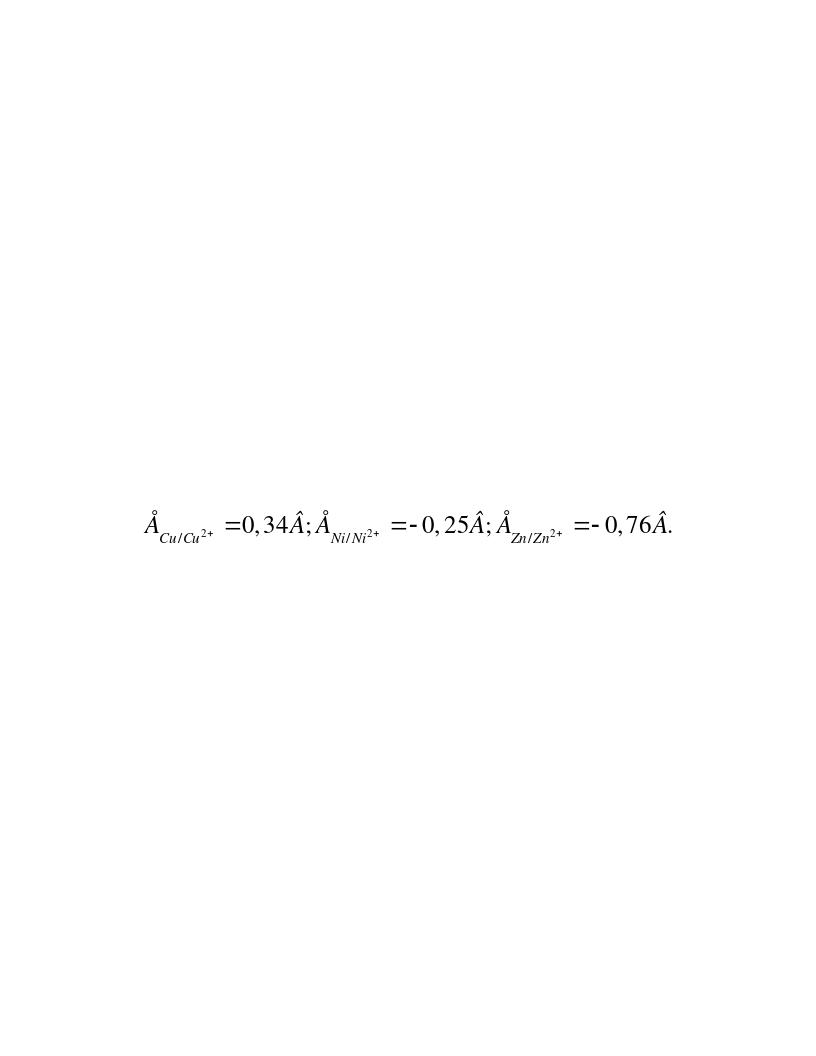
\includegraphics[width=0.8\textwidth]{image43}

As a result, in non-complexing media at copper reduction potentials, the
discharge of nickel and zinc at the cathode does not occur. This is the
basis, for example, for the process of electrolytic refining of copper,
where nickel and zinc, without being released at the cathode, accumulate
in sulfuric acid solutions. If complexing reagents are introduced into
the system - ammonia, citric acid, glycine, sufficiently stable
complexes with Cu\textsuperscript{2+}, Ni\textsuperscript{2+},
Zn\textsuperscript{2+} ions are formed in solution. Data on the
stability of these compounds are given in Table 1.

The formation of ammonia complexes leads to a shift in the reduction
potential of copper to a more negative region, and for copper this shift
was significant. The value of the reduction potential of copper still
remained positive than the potential for the release of nickel and zinc.
The recovery potential of nickel and zinc shifts to the positive region.

Table 1. Stability of copper, nickel and zinc complexes

\begin{longtable}[]{@{}
  >{\raggedright\arraybackslash}p{(\columnwidth - 12\tabcolsep) * \real{0.1464}}
  >{\raggedright\arraybackslash}p{(\columnwidth - 12\tabcolsep) * \real{0.1031}}
  >{\raggedright\arraybackslash}p{(\columnwidth - 12\tabcolsep) * \real{0.1328}}
  >{\raggedright\arraybackslash}p{(\columnwidth - 12\tabcolsep) * \real{0.1480}}
  >{\raggedright\arraybackslash}p{(\columnwidth - 12\tabcolsep) * \real{0.1482}}
  >{\raggedright\arraybackslash}p{(\columnwidth - 12\tabcolsep) * \real{0.1484}}
  >{\raggedright\arraybackslash}p{(\columnwidth - 12\tabcolsep) * \real{0.1731}}@{}}
\toprule\noalign{}
\begin{minipage}[b]{\linewidth}\raggedright
Metal ion
\end{minipage} & \begin{minipage}[b]{\linewidth}\raggedright
lg K\textsubscript{1}
\end{minipage} & \begin{minipage}[b]{\linewidth}\raggedright
lg K\textsubscript{1,2}
\end{minipage} & \begin{minipage}[b]{\linewidth}\raggedright
lg K\textsubscript{1,2,3}
\end{minipage} & \begin{minipage}[b]{\linewidth}\raggedright
lg K\textsubscript{1,2,3,4}
\end{minipage} & \begin{minipage}[b]{\linewidth}\raggedright
lg K\textsubscript{1,2,3,4,5}
\end{minipage} & \begin{minipage}[b]{\linewidth}\raggedright
lg K\textsubscript{1,2,3,4,5,6}
\end{minipage} \\
\midrule\noalign{}
\endhead
\bottomrule\noalign{}
\endlastfoot
\multicolumn{7}{@{}>{\raggedright\arraybackslash}p{(\columnwidth - 12\tabcolsep) * \real{1.0000} + 12\tabcolsep}@{}}{%
Ammonia complexes} \\
Сu\textsuperscript{2+} & 3,99 & 7,33 & 10,06 & 12,03 & 11,43 & 8,9 \\
Ni\textsuperscript{2+} & 2,69 & 4,79 & 6,40 & 7,47 & 8,10 & 8,01 \\
Zn\textsuperscript{2+} & 2,18 & 4,43 & 6,74 & 8,70 & - & - \\
\multicolumn{7}{@{}>{\raggedright\arraybackslash}p{(\columnwidth - 12\tabcolsep) * \real{1.0000} + 12\tabcolsep}@{}}{%
Citrate complexes} \\
\multicolumn{7}{@{}>{\raggedright\arraybackslash}p{(\columnwidth - 12\tabcolsep) * \real{1.0000} + 12\tabcolsep}@{}}{%
{[}(CH\textsubscript{2})\textsubscript{2}C(OH)
(COO)\textsubscript{3}{]}\textsuperscript{3-}} \\
Сu\textsuperscript{2+} & 5,90 & - & - & - & - & - \\
Ni\textsuperscript{2+} & 5,40 & - & - & - & - & - \\
\multicolumn{7}{@{}>{\raggedright\arraybackslash}p{(\columnwidth - 12\tabcolsep) * \real{1.0000} + 12\tabcolsep}@{}}{%
{[}(CH\textsubscript{2})\textsubscript{2}C(OH)(COOH)(COO)\textsubscript{2}{]}\textsuperscript{2-}} \\
Сu\textsuperscript{2+} & 3,42 & - & - & - & - & - \\
Ni\textsuperscript{2+} & 3,30 & - & - & - & - & - \\
\multicolumn{7}{@{}>{\raggedright\arraybackslash}p{(\columnwidth - 12\tabcolsep) * \real{1.0000} + 12\tabcolsep}@{}}{%
{[}(CH\textsubscript{2})\textsubscript{2}C(OH)(COOH)\textsubscript{2}COO{]}\textsuperscript{-}} \\
Сu\textsuperscript{2+} & 2,26 & - & - & - & - & - \\
Ni\textsuperscript{2+} & 1,75 & - & - & - & - & - \\
\end{longtable}

These data were obtained for both copper and titanium stationary
electrodes. The polarization curves are shown in Figures 1-4. The
magnitude of the limiting current increased with an increase in the
concentration of metal ions. It should be noted that the limiting
currents on the titanium electrode were 5-10 times higher than the
corresponding values obtained on the copper electrode.

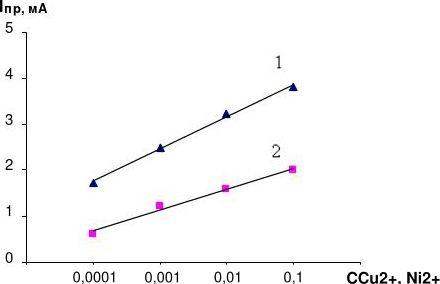
\includegraphics[width=0.8\textwidth]{image44}

\begin{longtable}[]{@{}
  >{\raggedright\arraybackslash}p{(\columnwidth - 0\tabcolsep) * \real{1.0000}}@{}}
\toprule\noalign{}
\begin{minipage}[b]{\linewidth}\raggedright
0,0001 0,001 0,01 0,1 C\textsubscript{Cu2+, Ni2+}
\end{minipage} \\
\midrule\noalign{}
\endhead
\bottomrule\noalign{}
\endlastfoot
\end{longtable}

Figure 1 - Dependence of the limiting reduction current of
Cu\textsuperscript{2+}(1) and Ni\textsuperscript{2+}(2) on a copper
electrode on the concentration of ions in solution. Ion concentrations,
mol/l: 0,0001; 0,001; 0,01; 0,1

The reduction of copper, nickel and zinc on a titanium electrode occurs
in a more negative potential range compared to copper (Table 2),
although the nature of the electrode does not significantly affect the
shape of the polarograms. The value of the half-wave potential on a
titanium electrode shifts to a less negative region with an increase in
the concentration of ions in the solution, whereas on a copper electrode
it remains at the same level. So, for example, when the copper
concentration changes from 10\textsuperscript{-4} to
10\textsuperscript{-1} M on a titanium electrode, the half-wave
potential changes from -0,68 V to -0,54 V, on a copper electrode it
remains at -0,54 V to -0,52 V.

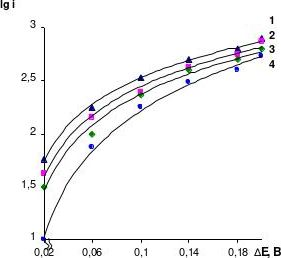
\includegraphics[width=0.8\textwidth]{image45}

Figure 2 - Dependence of lg I on the ΔE-reduction process of
Cu\textsuperscript{2+} concentration of 10\textsuperscript{-1} mol/l on
a titanium electrode with the addition of citric acid, g-eq/l: 1-0,01;
2-0,025; 3-0,05; 4-0,1

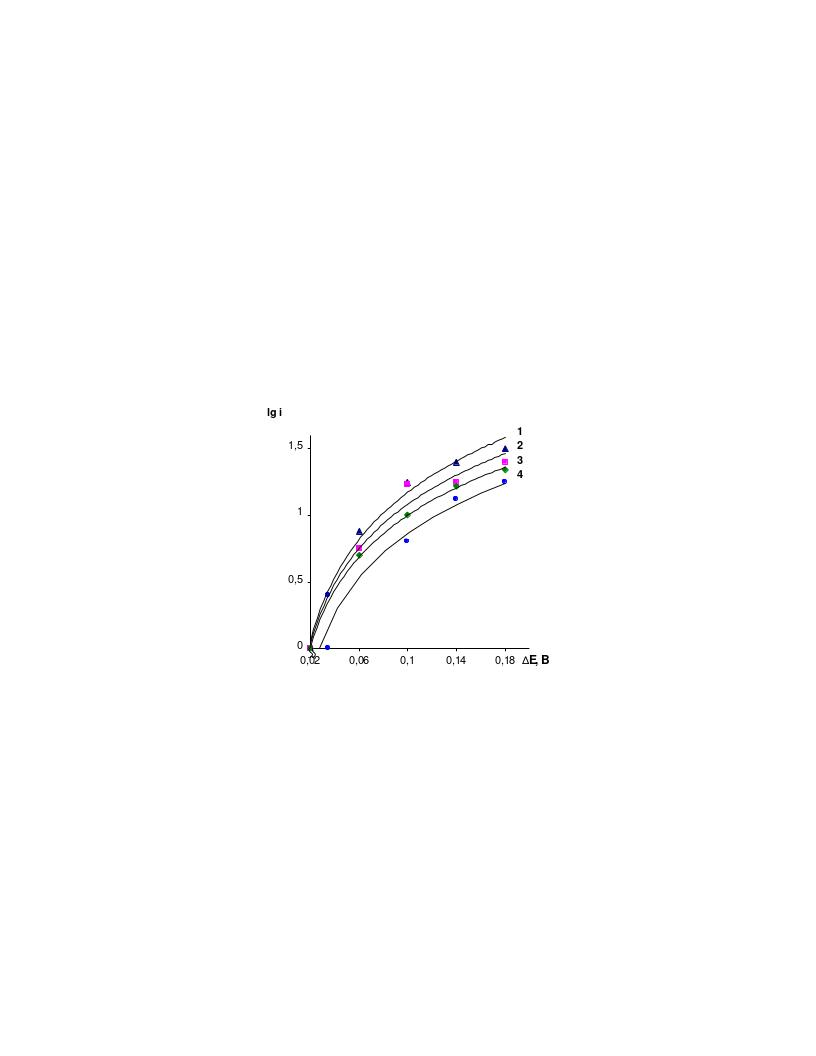
\includegraphics[width=0.8\textwidth]{image46}

Figure 3. Dependence of lg I on the ΔE-reduction process of
Ni\textsuperscript{2+} concentration of 10\textsuperscript{-1} mol/l on
a copper electrode with the addition of citric acid, g-eq/l: 1-0,01;
2-0,025; 3-0,05; 4-0,1

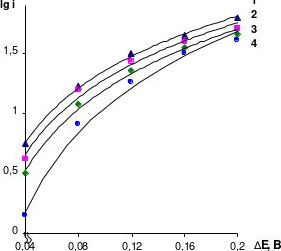
\includegraphics[width=0.8\textwidth]{image47}

Figure 4 - Dependence of lg I on the ΔE-reduction process of
Zn\textsuperscript{2+} concentration of 10\textsuperscript{-1} mol/l on
a copper electrode with the addition of citric acid, g-eq/l: 1-0,01;
2-0,025; 3-0,05; 4-0,1

Table 2 - The effect of the concentration of ammonia complexes on -E1/2
and I\textsubscript{pr}

\begin{longtable}[]{@{}
  >{\raggedright\arraybackslash}p{(\columnwidth - 10\tabcolsep) * \real{0.1310}}
  >{\raggedright\arraybackslash}p{(\columnwidth - 10\tabcolsep) * \real{0.1262}}
  >{\raggedright\arraybackslash}p{(\columnwidth - 10\tabcolsep) * \real{0.1359}}
  >{\raggedright\arraybackslash}p{(\columnwidth - 10\tabcolsep) * \real{0.1497}}
  >{\raggedright\arraybackslash}p{(\columnwidth - 10\tabcolsep) * \real{0.1497}}
  >{\raggedright\arraybackslash}p{(\columnwidth - 10\tabcolsep) * \real{0.3075}}@{}}
\toprule\noalign{}
\multicolumn{3}{@{}>{\raggedright\arraybackslash}p{(\columnwidth - 10\tabcolsep) * \real{0.3931} + 4\tabcolsep}}{%
\begin{minipage}[b]{\linewidth}\raggedright
Concentration, mol/l
\end{minipage}} &
\multirow{2}{*}{\begin{minipage}[b]{\linewidth}\raggedright
I\textsubscript{pr}, мA
\end{minipage}} &
\multirow{2}{*}{\begin{minipage}[b]{\linewidth}\raggedright
-Е\textsubscript{1/2}, В
\end{minipage}} &
\multirow{2}{*}{\begin{minipage}[b]{\linewidth}\raggedright
Cathode material
\end{minipage}} \\
\begin{minipage}[b]{\linewidth}\raggedright
Cu\textsuperscript{2+}
\end{minipage} & \begin{minipage}[b]{\linewidth}\raggedright
Ni\textsuperscript{2+}
\end{minipage} & \begin{minipage}[b]{\linewidth}\raggedright
Zn\textsuperscript{2+}.
\end{minipage} \\
\midrule\noalign{}
\endhead
\bottomrule\noalign{}
\endlastfoot
10\textsuperscript{-1} & & & 3,9 & 0,52 & \multirow{4}{*}{Cu} \\
10\textsuperscript{-2} & & & 3,15 & 0,54 \\
10\textsuperscript{-3} & & & 2,4 & 0,53 \\
10\textsuperscript{-4} & & & 1,7 & 0,54 \\
& 10\textsuperscript{-1} & & 3,3 & 0,58 & \multirow{4}{*}{Cu} \\
& 10\textsuperscript{-2} & & 2,85 & 0,60 \\
& 10\textsuperscript{-3} & & 2,3 & 0,59 \\
& 10\textsuperscript{-4} & & 1,8 & 0,56 \\
& & 10\textsuperscript{-1} & 2 & 0,62 & \multirow{4}{*}{Cu} \\
& & 10\textsuperscript{-2} & 1,5 & 0,58 \\
& & 10\textsuperscript{-3} & 1,2 & 0,58 \\
& & 10\textsuperscript{-4} & 0,7 & 0,565 \\
10\textsuperscript{-1} & & & 60 & 0,54 & \multirow{4}{*}{Ti} \\
10\textsuperscript{-2} & & & 47 & 0,60 \\
10\textsuperscript{-3} & & & 35 & 0,63 \\
10\textsuperscript{-4} & & & 22 & 0,66 \\
& 10\textsuperscript{-1} & & 51 & 0,62 & \multirow{4}{*}{Ti} \\
& 10\textsuperscript{-2} & & 40 & 0,64 \\
& 10\textsuperscript{-3} & & 29 & 0,63 \\
& 10\textsuperscript{-4} & & 18 & 0,65 \\
& & 10\textsuperscript{-1} & 44 & 0,68 & \multirow{4}{*}{Ti} \\
& & 10\textsuperscript{-2} & 34 & 0,67 \\
& & 10\textsuperscript{-3} & 25 & 0,64 \\
& & 10\textsuperscript{-4} & 15 & 0,635 \\
\end{longtable}

Citric acid shifts the copper half-wave potential to a more negative
area. If, in the absence of citric acid, the difference in the half-wave
potentials of copper and nickel is (on a titanium electrode) -0,08 V,
copper and zinc -- 0,14 V, then in the presence of citric acid in the
solution, the difference in the half-wave potentials of copper and
nickel is 0,015 V, copper and zinc -0,005 V. In this case, the reduction
potentials of copper, nickel and zinc converge. This promotes the joint
electrodeposition of Cu, Ni and Zn. Table 3 shows the data on the effect
of citrate ions on the reduction potentials and the magnitude of the
limiting current.

Table 3 -The effect of citric acid additions on -E\textsubscript{1/2}
and Ipr

\begin{longtable}[]{@{}
  >{\raggedright\arraybackslash}p{(\columnwidth - 12\tabcolsep) * \real{0.1422}}
  >{\raggedright\arraybackslash}p{(\columnwidth - 12\tabcolsep) * \real{0.1404}}
  >{\raggedright\arraybackslash}p{(\columnwidth - 12\tabcolsep) * \real{0.1310}}
  >{\raggedright\arraybackslash}p{(\columnwidth - 12\tabcolsep) * \real{0.1479}}
  >{\raggedright\arraybackslash}p{(\columnwidth - 12\tabcolsep) * \real{0.1381}}
  >{\raggedright\arraybackslash}p{(\columnwidth - 12\tabcolsep) * \real{0.1422}}
  >{\raggedright\arraybackslash}p{(\columnwidth - 12\tabcolsep) * \real{0.1582}}@{}}
\toprule\noalign{}
\multicolumn{3}{@{}>{\raggedright\arraybackslash}p{(\columnwidth - 12\tabcolsep) * \real{0.4136} + 4\tabcolsep}}{%
\begin{minipage}[b]{\linewidth}\raggedright
Concentration, mol/l
\end{minipage}} &
\multirow{2}{*}{\begin{minipage}[b]{\linewidth}\raggedright
C\textsubscript{citric acid}
\end{minipage}} &
\multirow{2}{*}{\begin{minipage}[b]{\linewidth}\raggedright
I\textsubscript{pr}, мA
\end{minipage}} &
\multirow{2}{*}{\begin{minipage}[b]{\linewidth}\raggedright
-Е\textsubscript{1/2}, В
\end{minipage}} &
\multirow{2}{*}{\begin{minipage}[b]{\linewidth}\raggedright
Cathode material
\end{minipage}} \\
\begin{minipage}[b]{\linewidth}\raggedright
Cu\textsuperscript{2+}
\end{minipage} & \begin{minipage}[b]{\linewidth}\raggedright
Ni\textsuperscript{2+}
\end{minipage} & \begin{minipage}[b]{\linewidth}\raggedright
Zn\textsuperscript{2+}
\end{minipage} \\
\midrule\noalign{}
\endhead
\bottomrule\noalign{}
\endlastfoot
10\textsuperscript{-1} & & & 0 & 3,9 & 0,52 & \multirow{5}{*}{Cu} \\
& & & 0,01 & 3,5 & 0,54 \\
& & & 0,025 & 3,2 & 0,53 \\
& & & 0,05 & 3,4 & 0,54 \\
& & & 0,1 & 3,9 & \\
& 10\textsuperscript{-1} & & 0 & 3,3 & 0,58 & \multirow{5}{*}{Cu} \\
& & & 0,01 & 2,6 & 0,60 \\
& & & 0,025 & 2,1 & 0,59 \\
& & & 0,05 & 1,6 & 0,56 \\
& & & 0,1 & 1,5 & \\
& & 10\textsuperscript{-1} & 0 & 2 & 0,62 & \multirow{5}{*}{Cu} \\
& & & 0,01 & 1,7 & 0,58 \\
& & & 0,025 & 1,5 & 0,58 \\
& & & 0,05 & 1,6 & 0,565 \\
& & & 0,1 & 1,3 & \\
10\textsuperscript{-1} & & & 0 & 60 & 0,54 & \multirow{5}{*}{Ti} \\
& & & 0,01 & 58 & 0,60 \\
& & & 0,025 & 56 & 0,63 \\
& & & 0,05 & 50 & 0,66 \\
& & & 0,1 & 40 & \\
& 10\textsuperscript{-1} & & 0 & 51 & 0,62 & \multirow{5}{*}{Ti} \\
& & & 0,01 & 48 & 0,64 \\
& & & 0,025 & 41 & 0,63 \\
& & & 0,05 & 41 & 0,65 \\
& & & 0,1 & 36,6 & \\
& & 10\textsuperscript{-1} & 0 & 44 & 0,68 & \multirow{5}{*}{Ti} \\
& & & 0,01 & 41 & 0,67 \\
& & & 0,025 & 38 & 0,64 \\
& & & 0,05 & 37 & 0,635 \\
& & & 0,1 & 32 & \\
\end{longtable}

The value of the limiting current decreased with an increase in the
concentration of the citric acid additive, especially when using a
titanium electrode. Glycine additives shift the half-wave potential of
both copper, nickel and zinc to a less negative region (by 0,078 V for
copper, 0,11 V for nickel, 0,12 V for zinc). But a significant gap
between them remains. The presence of glycine also led to a significant
change in the value of the limiting current at the electrodes (Table 4).

Changes in the voltammetric behavior of metals in the presence of citric
and aminoacetic (glycine) acids are associated with the noted processes
of complexation, the transition of metals from one complex form to
another.

Table 4 - The effect of glycine additives on -E\textsubscript{1/2} and
Ipr

\begin{longtable}[]{@{}
  >{\raggedright\arraybackslash}p{(\columnwidth - 12\tabcolsep) * \real{0.1365}}
  >{\raggedright\arraybackslash}p{(\columnwidth - 12\tabcolsep) * \real{0.1346}}
  >{\raggedright\arraybackslash}p{(\columnwidth - 12\tabcolsep) * \real{0.1273}}
  >{\raggedright\arraybackslash}p{(\columnwidth - 12\tabcolsep) * \real{0.1407}}
  >{\raggedright\arraybackslash}p{(\columnwidth - 12\tabcolsep) * \real{0.1330}}
  >{\raggedright\arraybackslash}p{(\columnwidth - 12\tabcolsep) * \real{0.1379}}
  >{\raggedright\arraybackslash}p{(\columnwidth - 12\tabcolsep) * \real{0.1899}}@{}}
\toprule\noalign{}
\multicolumn{3}{@{}>{\raggedright\arraybackslash}p{(\columnwidth - 12\tabcolsep) * \real{0.3985} + 4\tabcolsep}}{%
\begin{minipage}[b]{\linewidth}\raggedright
Concentration, mol/l
\end{minipage}} &
\multirow{2}{*}{\begin{minipage}[b]{\linewidth}\raggedright
Glycine\textsubscript{, г-экв/л}
\end{minipage}} &
\multirow{2}{*}{\begin{minipage}[b]{\linewidth}\raggedright
I\textsubscript{пр}, мA
\end{minipage}} &
\multirow{2}{*}{\begin{minipage}[b]{\linewidth}\raggedright
-Е\textsubscript{1/2}, В
\end{minipage}} &
\multirow{2}{*}{\begin{minipage}[b]{\linewidth}\raggedright
Cathode material
\end{minipage}} \\
\begin{minipage}[b]{\linewidth}\raggedright
Cu\textsuperscript{2+}
\end{minipage} & \begin{minipage}[b]{\linewidth}\raggedright
Ni\textsuperscript{2+}
\end{minipage} & \begin{minipage}[b]{\linewidth}\raggedright
Zn\textsuperscript{2+}.
\end{minipage} \\
\midrule\noalign{}
\endhead
\bottomrule\noalign{}
\endlastfoot
10\textsuperscript{-1} & & & 0 & 3,9 & 0,52 & \multirow{5}{*}{Cu} \\
& & & 0,01 & 3,4 & 0,54 \\
& & & 0,025 & 3,1 & 0,53 \\
& & & 0,05 & 3,3 & 0,54 \\
& & & 0,1 & 3,1 & \\
& 10\textsuperscript{-1} & & 0 & 3,3 & 0,58 & \multirow{5}{*}{Cu} \\
& & & 0,01 & 2,9 & 0,60 \\
& & & 0,025 & 2,5 & 0,59 \\
& & & 0,05 & 2,6 & 0,56 \\
& & & 0,1 & 2,65 & \\
& & 10\textsuperscript{-1} & 0 & 2 & 0,62 & \multirow{5}{*}{Cu} \\
& & & 0,01 & 1,7 & 0,54 \\
& & & 0,025 & 1,6 & 0,52 \\
& & & 0,05 & 1,8 & 0,525 \\
& & & 0,1 & 1,5 & 0,50 \\
\end{longtable}

\textbf{Conclusions.} Thus, if complexing reagents - ammonia, citric
acid, glycine - are introduced into the system, sufficiently stable
complexes with Cu\textsuperscript{2+}, Ni\textsuperscript{2+},
Zn\textsuperscript{2+} ions are formed in the solution. Glycine makes
the system more stable, which is associated with the formation of
homogeneous complexes. Citric acid reduces the limiting current, but the
equilibrium character remains unchanged. At the same time, the reduction
potentials of copper, nickel and zinc converge, which contributes to
their joint electrodeposition. The results of the research can be used
to solve problems in the field of processing solutions derived from the
cycle of electrolytic refining of copper.

\textbf{Литература}

1. Омаров Х.Б., Жарменов А.А., Сагиндыкова З.Б. Мышьяк в гидрохимических
процессах медного производства. -- Караганда: Изд-во КарГУ, 2007. -- 167
с.

2. Жарменов А.А., Милицин В.В., Омаров Х.Б. и др. Опытно-промышленные
испытания аммиачной технологии переработки медного электролита на АО
«Жезказганцветмет» // Промышленность Казахстана. 2000. - №3.-- С. 51-93.

3. Cumbal L. Sen Gupta A.K. Arsenic removal using polymer-supported
hydrated lron (III) oxide nanoparticles: role of donnan membrane effect
// Environ. Sci. Technol. - 2005, №39. - P. 6508-6515.

4. Шаталов В.В., Смирнова Н.М., Глухова Л.П., Савельева Т.И. Мембранные
процессы в гидрометаллургии // Цветные металлы. - 2003. - №4. - С.
53-57.

5. Тодоров С.А., Лайнер Ю.А., Медведев А.С. Утилизация
низкоконцентрированных растворов с использованием электродиализа //
Цветная металлургия. - 2004. - №3. - С. 37-39.

6. Шапошник В.А., Котов В.,В, Кобелева Н.С. Влияние плотности тока на
эффективность разделения ионов при электродиализе // Прикладная химия.
-- 1980. - №5. -- С. 1058-1061.

7. Разделение и очистка веществ методом электродиализа с ионообменными
мембранами // РЖХ. -- 1986. - 5Л3Б.

8. Певницкая М.В., Гнусин Н.П., Лаврова Т.А. Электрический перенос ионов
через катионитовую мембрану в смешанных растворах солей // Известия СO
АН CССР, Серия химических наук. -- 1965. - №7. -- С. 13-18.

9. Жарменов А.А. Электродиализная переработка растворов
электролитического рафинирования меди: автореф\ldots{} канд. техн. наук:
- Алма-Ата, 1982. -21с.

10. Жарменов А.А., Шарипов М.Ш. Избирательность катионитовых мембран в
сернокислых растворах никеля и меди //Прикладная химия. -- 1985.
--№2.-С.275-278.

11. Agraz R., Sevilla M.T. and Hernandez L. Chemically modified
electrode for the simultaneous determination of trace metals and
speciation analysis. Anal. Chim. Acta. 1993. Vol. 273. P. 205.

12. Багхери А., Маранд М.Х. Вольтамперометрическое и потенциометрическое
определение Cu\textsuperscript{2+} с помощью электрохимического сенсора
на основе сверхокисленного полипиррола. Электрохимия. 2020. Т. 56. № 6.
С. 483-493.

13. Касач А.А., Харитонов Д.С., Радченко С.Л. и др. Исследование влияния
параметров импульсного электролиза на процесс электроосаждения сплава
медь-олово из сульфатного электролита. Электрохимия. 2020. Т. 56. №9.
С.820-830.

14. Zanganeh A.R. and Amini M.K. Polypyrrole-modified electrodes with
induced recognition sites for potentiometric and voltammetric detection
of copper (II) ion. Sens. Act. B. 2008/ Vol. 135. P. 358.

15. Meudre C., Ricg I., Hihn J.Y. and others. Absorption of gelatin
during electrodeposition of copper and tin-copper alloys from acid
sulfate electrolyte. Surf. Coat. Tech., 2014. Vol. 252. P.93.

16. Желис Х.П. Винкавичус И.И. Химическое осаждение никелевых сплавов //
Труды АН Лит ССР. -1985 Б. - № 61.151. -- С.3-9.

17 А.С. 1148903 СССР. Способ переработки медного электролита
электролизом / А.А. Жарменов и др.; опубл. 1985, Бюл. №13.

\textbf{References}

1. Omarov Kh.B., Zharmenov A.A., Sagyndykova Z.B. Myshyak v
gidrochemitheskikh processakh mednogo proizvodstva. -Karaganda:Izd-vo
KarGU, 2007. -167s.

2. Zharmenov A.A., Milicin V.V., Omarov Kh.B. i dr. Opytno-promyshlennye
ispytania ammiathnoi technologii pererabotki mednogo electrolita na AO
«Zhezkazgancvetmet» // Promyshlennost Kazakhstana. 2000. -№3. -S. 51-93.

3. Cumbal L. Sen Gupta A.K. Arsenic removal using polymer-supported
hydrated lron (III) oxide nanoparticles: role of donnan membrane effect
// Environ. Sci. Technol. - 2005, №39. - P. 6508-6515.

4. Shatalov V.V., Smirnova N.M., Glukhova L.P., Savelieva T.I.
Membrannye process v gidrometallurgii // Cvetnye metally. -- 2003. -№3.
-S. 53-57.

5. Todorov S.A., Lainer Ua.A., Medvedev A.S. Utilizaciya
nizkoconcenrirovannykh rastvorov s ispolzovaniem electrodializa //
Cvetnaya metallurgiya. -- 2004. - №3. -S. 37-39.

6. Shaposhnik V.A., Kotov V.V., Kobeleva N.S. Vliyanie plotnosti toka na
effectibnost razdeleniya ionov pri electrodialize // Pricladnaya
chimiya. -- 1980. - №5. -- S. 1058-1061.

7. Razdelenie i othistka veschestv metodom electrodializa s
ionoobmennymi membranami // RZhCh. -- 1986. -- 5L3B.

8. Pevnickaya M.V., Gnusin N.P., Lavrova T.A. Electritheskii perenos
ionov therez kationitovuua membranu v smeshannych rastvorach solei //
Izvestiya SO AN SSSR, Seriya chimitheskich nauk. -- 1965. - №7. -- S.
13-18.

9. Zharmenov A.A. Electrodializnaya pererabotka rastvorov
electrolititheskogo rafinirovaniya medi: avtoref\ldots kand. techn.
nauk: - Alma-Ata, 1982. -21s.

10. Zharmenov A.A., Sharipov M.Sh. Izbiratelnost kationitovych membran v
sernokislych rastvorach nicelya i medi // Pricladnaya chimiya. . --
1985. --№2.-S.275-278.

11. Agraz R., Sevilla M.T. and Hernandez L. Chemically modified
electrode for the simultaneous determination of trace metals and
speciation analysis. Anal. Chim. Acta. 1993. Vol. 273. P. 205.

12. Bagcheri A., Marand M.Ch. Voltamperometritheskoe i
potenciometritheskoe opredelenie Cu\textsuperscript{2+} s pomoschua
electrochimitheskogo sensora na osnove sverchokislennogo polipirolla.
Electochimiya. 2020. Т. 56. № 6. S. 483-493.

13. Kasath A.A., Charitonov D.S., Radthenko S.L. i dr. Issledovanie
vliyaniya parametrov impulsnogo electroliza na process electroosagdeniya
splava med-olovo iz sulfatnogo electrolita. Electochimiya. 2020. Т. 56.
№9. S.820-830.

14. Zanganeh A.R. and Amini M.K. Polypyrrole-modified electrodes with
induced recognition sites for potentiometric and voltammetric detection
of copper (II) ion. Sens. Act. B. 2008/ Vol. 135. P. 358.

15. Meudre C., Ricg I., Hihn J.Y. and others. Absorption of gelatin
during electrodeposition of copper and tin-copper alloys from acid
sulfate electrolyte. Surf. Coat. Tech., 2014. Vol. 252. P.93.

16. Zhelis Ch.P., Vinkavithus I.I. Chimicheskoe osazhdenie nicelevych
splavov // Trudy AN Lit. SSR. -1985 B. - № 61.151. -- S.3-9.

17 A.S. 1148903 SSSR. Sposob pererabotki mednogo electrolita
electrolizom / A.A.Zharmenov i dr.; opubl. 1985, Bual. №13.

\emph{\textbf{Information about authors}}

Omarov Khylysh Beisenovich, Doctor of Technical Sciences, Professor,
Professor of the Department of Chemistry, Chemical Technology and
Ecology, Kazakh University of Technology and Business, Republic of
Kazakhstan, Astana, e-mail:
\href{mailto:homarov1963@mail.ru}{\ul{homarov1963@mail.ru}}

Nurtai Zhadyra Tastenbekovna, PhD, Associate Professor of the Department
of Chemistry, Chemical Technology and Ecology, Kazakh University of
Technology and Business, Republic of Kazakhstan, Astana, e-mail:
\href{mailto:zhadira_nurtai@mail.ru}{\ul{zhadira\_nurtai@mail.ru}}

Kopylov Nikolai Ivanovich, Doctor of Technical Sciences, Professor,
Leading Researcher, Institute of Solid State Chemistry and
Mechanochemistry, Siberian Branch of the Russian Academy of Sciences,
Russia, Novosibirsk, e-mail:
\href{mailto:kopylov@narod.ru}{\ul{kopylov@narod.ru}}

\emph{\textbf{Сведения об авторах}}

Омаров Хылыш Бейсенович, доктор технических наук, профессор, профессор
кафедры химии, химической технологии и экологии Казахского университета
технологии и бизнеса, Республика Казахстан, г. Астана, e-mail:
\href{mailto:homarov1963@mail.ru}{\ul{homarov1963@mail.ru}}

Нұртай Жадыра Тастенбековна, доктор PhD, ассоциированный профессор
кафедры химии, химической технологии и экологии Казахского университета
технологии и бизнеса, Республика Казахстан, г. Астана, e-mail:
\href{mailto:zhadira_nurtai@mail.ru}{\ul{zhadira\_nurtai@mail.ru}}

Копылов Николай Иванович, доктор технических наук, профессор, ведущий
научный сотрудник Института химии твердого тела и механохимии Сибирского
отделения Российской Академии наук, Россия, г. Новосибирск, e-mail:
kopylov@narod.ru

\textbf{Производственные и обрабатывающие отрасли}

\textbf{МРНТИ: 52.13.17; 20.51.23; 87.15.15; 44.01.75}

\begin{quote}
\textbf{НАПРАВЛЕНИЯ ПОВЫШЕНИЯ ЭНЕРГОЭФФЕКТИВНОСТИ НА ОТКРЫТЫХ
РАЗРАБОТКАХ МЕСТОРОЖДЕНИЙ ПОЛЕЗНЫХ ИСКОПАЕМЫХ}
\end{quote}

\textbf{С.Ж. Галиев\textsuperscript{1*}, Е.Т.Утешов\textsuperscript{1*},
Д.А. Галиев\textsuperscript{1}, Ж.С. Бексапин \textsuperscript{2}}

Институт горного дела им. Д.А.Кунаева РГП «НЦ КПМС» МИИР РК, г. Алматы,
Казахстан,

ТОО «Qazakstan smart technology», г. Алматы, Казахстан,

email: seitgaligaliyev@mail.ru

Статья посвящена актуальной теме, в которой сочетаются проблемные
вопросы энергоэффективности и низкоуглеродного развития горного
производства. В ней раскрываются подходы и методические аспекты анализа
и оценки энергоэффективности горных предприятий с открытым способом
освоения месторождений твёрдых полезных ископаемых. В основе методологии
лежит процессный подход, базирующийся на процессах цифровизации,
развития информационных технологий и соответствующего
программно-методического обеспечения с применением эффективного для
решения данного рода задач метода имитационного моделирования. В статье
раскрываются результаты проведения комплексных технико-технологических и
энерго- аудитов, позволяющих выявлять реальный потенциал повышения
энергоэффективности и направления его реализации с последующей
выработкой комплекса конкретных мер в данном направлении. Одними из
основных выводов является вывод о наличии существенно потенциала
повышения энергоэффективности (10-15\%) и обоснование необходимости
формирования на горных предприятиях автоматизированных систем энерго- и
экологического мониторинга, позволяющих, с одной стороны, своевременно и
целенаправленно вырабатывать оперативные управленческие меры, а с
другой, повысить эффективность реализации принципа экологичности и
безопасности в процессе технологической модернизации горных производств.

\textbf{Ключевые слова:} Открытые горные работы, геотехнологический
комплекс,

экологические выбросы, энергоэффективность, энергосбережение, экономика,
оптимизация, автоматизация.

\textbf{ПАЙДАЛЫ ҚАЗБАЛАР КЕН ОРЫНДАРЫН АШЫҚ ИГЕРУДЕГІ ЭНЕРГИЯ
ТИІМДІЛІГІН АРТТЫРАУ БАҒЫТТАРЫ}

\textbf{С.Ж. Ғалиев\textsuperscript{1*}, Е.Т. Өтешов\textsuperscript{1},
Д.А. Ғалиев\textsuperscript{1}, Ж. С. Бексапин\textsuperscript{2}}

Д. А. Қонаев атындағы Тау-кен институты. Д. А. Қонаева ҚР ИИДМ

"КПМС ҰО" РМК, Алматы қ., Қазақстан, "Qazakstan smart technology" ЖШС,
Алматы қ., Қазақстан,
е-mail:~\href{https://e.mail.ru/compose/?mailto=mailto\%3aseitgaligaliyev@mail.ru}{seitgaligaliyev@mail.ru}~

Мақала энергия тиімділігі мен тау-кен өндірісінің төмен көміртекті
дамуының проблемалық мәселелерін біріктіретін өзекті тақырыпқа арналған.
Онда қатты пайдалы қазбалар кен орындарын игерудің ашық тәсілімен
тау-кен кәсіпорындарының энергия тиімділігін талдау мен бағалаудың
тәсілдері мен әдістемелік аспектілері ашылады. Әдістеме цифрландыру,
ақпараттық технологияларды дамыту және осы типтегі міндеттерді шешуде
тиімді модельдеу әдісін қолдана отырып, тиісті бағдарламалық-әдістемелік
қамтамасыз ету процестеріне негізделген процестік тәсілге негізделген.
Мақалада энергия тиімділігін арттырудың нақты әлеуетін және оны іске
асыру бағытын анықтауға мүмкіндік беретін кешенді
техникалық-технологиялық және энергетикалық аудиттерді жүргізу
нәтижелері, содан кейін осы бағытта нақты шаралар кешені әзірленеді.
Негізгі тұжырымдардың бірі-энергия тиімділігін арттырудың айтарлықтай
әлеуетінің болуы туралы қорытынды (10-15\%) және негіздеме.

\textbf{Түйінді сөздер:} Ашық тау-кен жұмыстары, геотехнологиялық кешен,
экологиялық шығарындылар, энергия тиімділігі, энергия үнемдеу,
экономика, оңтайландыру, автоматтандыру.

\textbf{DIRECTIONS OF ENERGY EFFICIENCY IMPROVEMENT IN OPEN PIT MINING
OF MINERAL DEPOSITS}

\textbf{S.Zh. Galiev\textsuperscript{1*}, E.T.
Uteshov\textsuperscript{1}, D.A. Galiev\textsuperscript{1},Zh.S
Beksapin\textsuperscript{2}}

Mining Institute after D.A. Kunayev of RSE "NC KPMC" MIIR RK, Almaty,
Kazakhstan, Almaty, Kazakhstan, Qazakstan smart technology" LLP, Almaty,
Kazakhstan,

е-mail:~\href{https://e.mail.ru/compose/?mailto=mailto\%3aseitgaligaliyev@mail.ru}{seitgaligaliyev@mail.ru}~

The article is devoted to the actual topic, which combines the
problematic issues of energy efficiency and low-carbon development of
mining production. It reveals the approaches and methodological aspects
of the analysis and assessment of energy efficiency of mining
enterprises with the open-pit method of development of deposits of solid
minerals. The methodology is based on the process approach based on the
processes of digitalization, development of information technologies and
corresponding software and methodological support with the use of
simulation modeling method effective for solving this kind of problems.
The article reveals the results of comprehensive technical and
technological and energy audits, which allow to identify the real
potential of energy efficiency and areas of its implementation with the
subsequent development of a set of specific measures in this direction.
One of the main conclusions is the conclusion that there is a
significant potential to increase energy efficiency (10-15\%) and the
rationale for the need to form automated energy and environmental
monitoring systems at mining enterprises, allowing, on the one hand,
timely and targeted development of operational management measures, and
on the other hand, to improve the effectiveness of the principle of
environmental and safety in the process of technological modernization
of mining production.

\textbf{Keywords:} open-pit mining, geotechnological complex,
environmental emissions, energy efficiency, energy conservation,
economy, optimization, automation.

\textbf{Введение.} Вопросы энергоэффективности традиционно имеют высокую
актуальность, которая в последние десятилетия усиливается проблемами
экологии и глобального потепления. Эти вопросы становятся центральной
темой ежегодных глобальных форумов, проходящих с участием
правительственных делегаций стран мира. Казахстан в этом плане
присоединился к международным инициативам приняв Указом Президента
Республики Казахстан от 2 февраля 2023 года за № 121 Стратегию
достижения углеродной нейтральности Республики Казахстан до 2060 года.
Для Казахстана проблема энергоэффективности актуальна и в связи с тем,
что основным источником энергии в стране является уголь. Практически всё
промышленное производство страны подпадает под экологические санкции,
выдвигаемые международным сообществом, и проблема снижения экологических
выбросов жёстко коррелирует с задачами повышения энергоэффективности.
Особенно жёстко данный вопрос стоит перед горнодобывающей отраслью
экономики, являющейся одной из самых энергозатратных, а также и одним из
крупнейших загрязнителей окружающей среды.

По результатам ряда проведённых исследований, очевиден существенный
потенциал повышения энергоэффективности, реализация которого сопряжена
со снижением себестоимости горнотранспортных работ в среднем на 10-15\%.
Для Казахстана это принципиально важно не только по экономическим
аспектам, но также в связи с повышением рентабельности освоения
отечественной минерально-сырьевой базы и выполнением принятых
международных обязательств о снижении выбросов к 2030 г. на 15\%
относительно уровня выбросов 1990 г. (безусловная цель) и доведение
сокращения на 25 \% при условии получения международной поддержки на
декарбонизацию экономики (условная цель) {[}1{]}.

Для Казахстана достижение углеродной нейтральности является достаточно
амбициозной задачей, которую планируется достичь через реализацию
инициатив по трем ключевым направлениям, одно из которых -
декарбонизация отраслей и процессов, связанных с ископаемым топливом
{[}2{]}. При этом, выбросы парниковые газы, связанные с ископаемым
топливом, будут сокращены посредством перехода от использования
ископаемого топлива и его производных к альтернативным и возобновляемым
источникам энергии, путём повышения энергоэффективности и
энергосбережения, взятием курса на дальнейшую электрификацию (замещения
установок, сжигающих топливо, на технологии, работающие на основе
электроэнергии).

\emph{Потенциал повышения энергоэффективности и достижения углеродной
нейтральности в горнодобывающей отрасли Казахстана:}

По данным казахстанской статистики на современном этапе 86,6\% выбросов
в РК приходится на промышленность, в т.ч. на горнодобывающую - 53,45\%
(11, 2 млн. тонн в год). Энергоемкость продукции ГМК превышает
аналогичный показатель ОЭСР более чем в 2 раза. Наибольшие выбросы и
расход топлива приходятся на автотранспорт. В общем объеме
производственных затрат ГМК, расходы на дизельное топливо и
электроэнергию составляют около 50\%.

Если проанализировать возможные направления повышения
энергоэффективности и снижения углеродоёмкости горного производства, то
их можно сформулировать следующим образом:

- за счёт оптимизации производственных и технологических процессов --
потенциал до 15\% с достижением экономических эффектов в виде снижения
себестоимости горнотранспортных работ до 10-15\%/год при попутном
повышении технологической культуры;

- перевод автотранспорта на газодизельные двигатели -- снижение до
25-30\% экологических выбросов, сопровождающееся аналогичным где-то
снижением себестоимости горнотранспортных работ;

- адаптация транспортной инфраструктуры и структуры энергосетей со
структурой минерально-сырьевой базы Республики Казахстан -- потенциал
снижения объёмов выбросов СО2 и снижения себестоимости около 5-10\%;

- разработка технологий снижения (декарбонизация) выбросов загрязняющих
веществ (УХУ: улавливание до 90\%, хранение и утилизация -- до 100\%);

- совершенствование технологий в рамках процесса технологической
модернизации -- долгосрочная перспектива с потенциалом до 100\%
(экскаваторно-конвейерные комплексы, скиповые подъёмники и др.);

- освоение технологий подземного скважинного выщелачивания (ПСВ) для
освоения месторождений руд цветных и чёрных металлов -- до 100\%;

- комплексное освоение минерально-сырьевой базы Казахстана -- помимо
значительного снижения углеродоёмкости, снижение затрат на извлечение
сокращается в разы;

- перевод системы энергообеспечения ГМК РК на альтернативные и
возобновляемые источники (водород, солнечная и ветряная энергия, водные
электростанции, урановое производство и атомные электростанции) -- до
100\% снижение углеродоёмкости;

- разработка нанотехнологий освоения месторождений полезных ископаемых
-- касается практически всей минерально-сырьевой базы -- потенциал до
100\%.

В приведенном перечне, первые два направления могут быть
первоочередными, так как не требуют каких-либо особых дополнительных
вливаний. Тут достаточно поддержки развития программно-методического
обеспечения на основе пооперационной цифровизации и углубленной
аналитики в рамках широко применяемых сегодня инструментов
финансирования науки. С этой целью необходимо привлечение таких
инструментов инновационно-индустриального развития и стимулирования
технологической модернизации, как проведение комплексных
технико-технологических аудитов и совершенствование энергоаудитов, что
позволит своевременно и точно определять имеющийся потенциал,
направления и меры по его своевременной реализации.

\textbf{Материалы и методы - методология оценки энергоэффективности.}
Комплексный технико-технологический аудит проектных решений по
формированию, а также эксплуатируемых геотехнологических комплексов
осуществляется на основе системного подхода, при котором одним из
ключевых факторов является адекватный учёт процессности в управлении
горнотранспортными работами. В свою очередь, этот подход основывается и
реализуется в рамках теории и методологии модернизации, индустриализации
и технологической модернизации {[}3-4{]}.

Рассматриваемый подход предполагает использование наиболее эффективного
на данном направлении метода имитационного логико-статистического
моделирования, обеспечивающего достоверное воспроизведение порядка и
последовательности основных технологических и
организационно-экономических операций в конкретных горнотехнических,
горно-геологических, горно-геометрических, организационных и
экономических условиях. В настоящее время данные подход и метод уже боле
40 лет широко применяются для технико-экономического анализа
эффективности функционирования геотехнологических комплексов на открытых
разработках с использованием цикличных технологий с автомобильным,
железнодорожным и комбинированным автомобильно-железнодорожным видами
транспорта горной массы.

Основной целью комплексного технико-технологического аудита является
оценка эффективности, включая энергоэффективность, функционирования
геотехнологического комплекса, выявление имеющегося потенциала,
направлений и установления мер по его реализации.

В случае рассмотрения геотехнологического комплекса с применением
автотранспорта, основными элементами его, как системы, являются
карьерная автотрасса, экскаваторный и автомобильный парки, геометрия
карьерного пространства, принятые на предприятии организационные меры и
нормативы. По автотрассе адекватно учитываются её структура со всеми
технологическими особенностями и фактического расположения блок-участков
в карьерном пространстве, их геометрия (уклон, протяжённость,
криволинейность) и качество применяемого дорожного покрытия, а также
затраты на их формирование и поддержание в рабочем состоянии. По
экскаваторному и автомобильному парку достоверному учёту подлежат
основные паспортные технико-технологические характеристики (ёмкость
кузова и ковша, КПД трансмиссии и двигателей, их мощностные
характеристики, сроки эксплуатации и принятые нормативы по
эксплуатации), модели и число работающего и списочного парков, а также
их стоимостные характеристики (остаточная стоимость, цены, нормы
амортизации). Параметры принципиальных характеристик карьерного
пространства учитываются благодаря использованию графических документов,
полученных с использованием специализированной программы AutoCAD.

Одним из важнейших направлений комплексного технико-технологического
аудита является оценка его энергоэффективности. Энергоёмкость основных
технологических процессов при освоении месторождений твёрдых полезных
ископаемых открытым способом и с применением цикличных технологий добычи
занимает в среднем 60-70 \% в общей себестоимости горнотранспортных
работ. При заданных технологиях освоения месторождений, когда определены
направления и порядок ведения добычных и вскрышных работ, основные
направления поиска потенциала снижения энергоёмкости технологических
связаны с соответствующим выбором моделей основного горного и
транспортного оборудования, режимом и условиями их эксплуатации
{[}5-11{]}.

В свою очередь, исследование режимов эксплуатации основного горного и
транспортного оборудования требует соответствующих методов и подходов,
позволяющих вести адекватный учёт основных влияющих на результативность
работы горнотранспортного комплекса факторов, как это показано на
рисунке 1. Это позволяет оценивать энергоэффективность исходя из
адекватного учёта пооперационного расхода энергии и характера интеграции
этих долей энергии в формирующиеся энергопотоки технологического
процесса в целом.

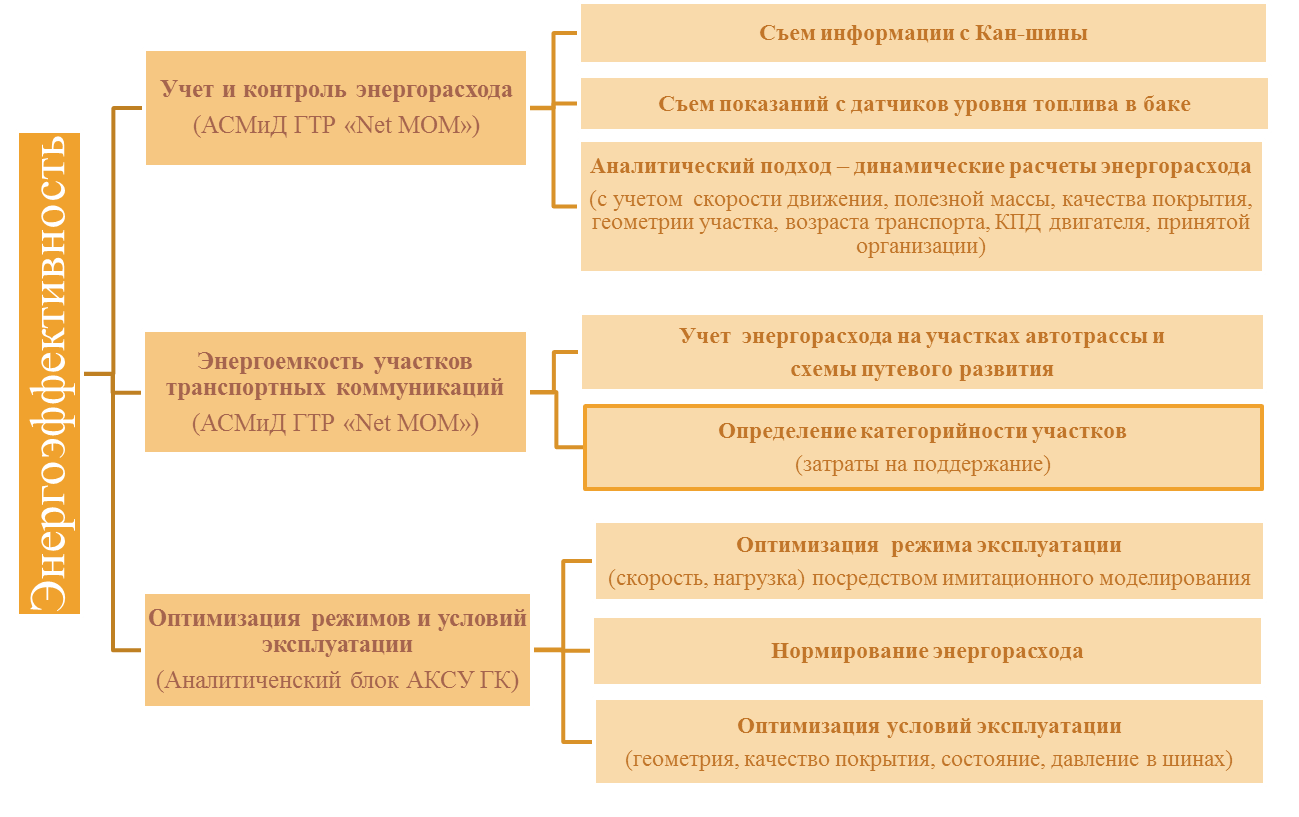
\includegraphics[width=0.8\textwidth]{image48}

Рис. 1 -- Концепция энергосбережения на открытых разработках

Энергоэффективность предполагает не только простое снижение
энергорасхода, а прежде всего в увязке с общей эффективностью
функционирования геотехнологического комплекса, которая оценивается с
применением комплекса технико-экономических критериев. В связи с этим,
принципиально важным в процессе анализа и оценки энергоэффективности
исследуемых технологических процессов основываться на адекватном учёте
пооперационных затрат горнотранспортного процесса и технического
состояния машин. Одним из принципиальных показателей в этом плане
является КПД двигателя автосамосвала, который имеет зависимость своего
значения от возраста эксплуатируемых машин (см. рис.2). Это позволяет
достоверно оценивать экономическую эффективность энергорасхода,
способность энергии к обеспечению повышенной производительности, а,
следовательно, устанавливать уровень его целесообразности. Для этих
целей применяется методология экономики процессного управления.

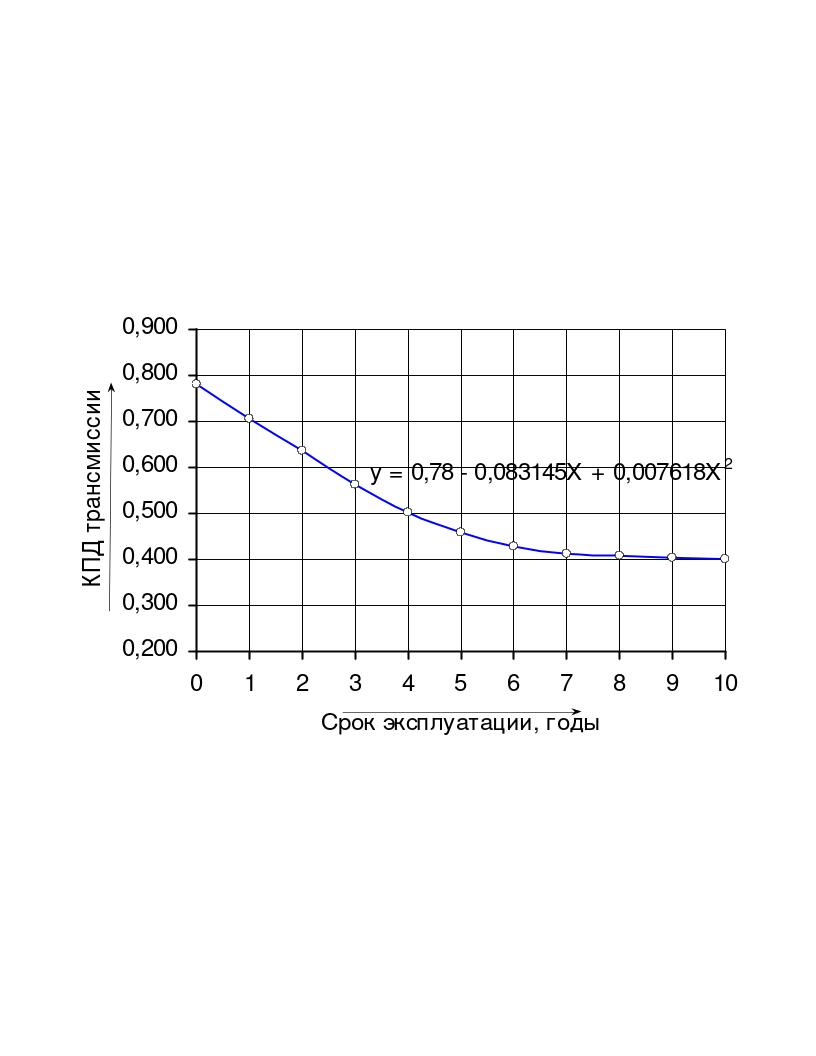
\includegraphics[width=0.8\textwidth]{image49}

Рис. 2 - Зависимость КПД двигателя автосамосвала от срока эксплуатации

Другим важным моментом в применяемом подходе является адекватный
динамический подход к учёту энергорасхода автосамосвалами в зависимости
от паспортных тяговых характеристик двигателей и трансмиссии машин (см.
рисунок 3), позволяющих воспроизводить реальную процессную взаимосвязь в
динамике скорости движения автосамосвала и энергорасхода в зависимости
от режима и условий их эксплуатации -- качества дорожного покрытия,
геометрия по участкам автотрассы, техническое состояние и режим загрузки
автосамосвалов (вровень, «с шапкой», «без шапки»).

По специализированным карьерным автосамосвалам тяговые характеристики
являются паспортными, полученные заводом изготовителем, а по
автосамосвалам не специализированным они были получены путём перевода из
имеющейся формы отражения тяговых характеристик (часто в место тяговых
усилий указываются обороты двигателя). Данный способ учёта энергорасхода
является наиболее достоверным и обеспечивает адекватную чувствительность
к изменениям всех обозначенных принципиальных факторов, обуславливающих
энергорасход. Тяговые характеристики вшиты в модели автосамосвалов и
своевременно используются алгоритмом в процессе моделирования.

По погрузочному оборудованию, учёт энергорасхода (электричество,
дизельное топливо) осуществляется в зависимости от КПД двигателя,
времени циклов, ёмкости ковша и плотности экскавируемых горных пород с
учётом соответствующего коэффициента разрыхления.

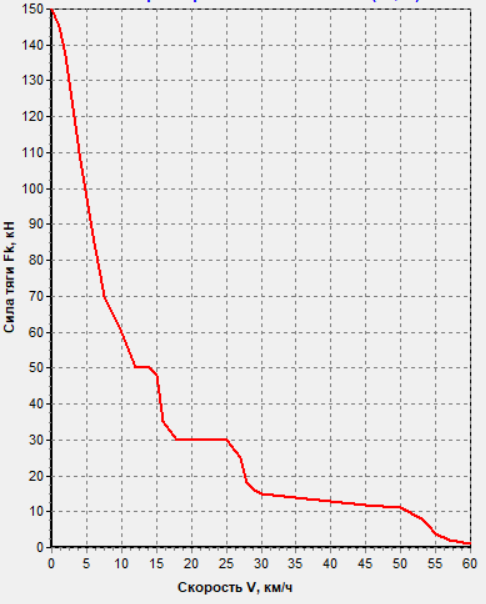
\includegraphics[width=0.8\textwidth]{image50}

Рис. 3. - Тяговые характеристики автосамосвалов БелАЗ-7540

Для адекватного учёта энергорасходов на участках транспортных
коммуникаций необходимо достоверное воспроизведение их структуры и
характеристик качественных и технологических, как это показано на
рисунке 4. С этой целью используется план (фактический или проект)
горных работ, выполненный в AutoCAD либо полученный с использованием
широко ныне используемых летательных аппаратов дронов, которые позволяют
с максимальной точностью воспроизводить на имитационных цифровых моделях
в трёхмерном пространстве горно-геометрические параметры. С планов
горных работ и из пояснительных записок по ним берутся необходимые
организационные и технико-технологические характеристики по ним. Это
позволяет точно позиционировать в карьерном пространстве все имеющиеся
пункты погрузки-выгрузки и перегрузки горной массы, а следовательно,
адекватно учитывать структуры формируемых рудо- и породо- потоков.

Таким образом, проведение комплекса исследований предполагается на
основе системного подхода с применением методологии имитационного
моделирования исследуемых горнотранспортных процессов, обеспечивающих
адекватный учёт порядка и последовательности операций основных
технологических процессов с достоверным учётом конкретных
горнотехнических, горно-геометрических, горно-геологических,
организационных и экономических условий функционирования основного
технологического комплекса разрезов {[}6-10{]}.

\includegraphics[width=0.8\textwidth]{image51}

Рис. 4 - План разреза «Центральный» с встроенной структурой модели
горнотранспортного комплекса

Применяемая в процессе имитационного моделирования и исследований
методология формирования экономико-математических моделей обеспечивает
адекватный учёт порядка и последовательности пооперационных затрат на
поддержание работы горнотранспортного комплекса.

Одно из достоинств применяемого подхода заключается в практически
достоверном учёте общего режима и календаря эксплуатации
горнотранспортных комплексов разрезов, что имеет принципиальное значение
для обеспечения точности основных технико-экономических расчётов и
эффективности комплекса предлагаемых мер.

\textbf{Результаты и обсуждение -} направления повышения эффективности.

Возможные в рамках данного направления повышения энергоэффективности под
направления можно увидеть по таблице 1, где на примере одного из
исследуемых объектов, среди с общепроизводственных мероприятий,
наибольшую долю (до 90\%) имеющегося потенциала имеют улучшение качества
покрытия внутрикарьерных дорог, внедрение автоматизированной системы
мониторинга энергорасхода, и оптимизации парка автосамосвалов, а также
режимов и условий их эксплуатации.

Таблица 1. План энергосберегающих мероприятий по предприятию

\begin{longtable}[]{@{}
  >{\raggedright\arraybackslash}p{(\columnwidth - 8\tabcolsep) * \real{0.0551}}
  >{\raggedright\arraybackslash}p{(\columnwidth - 8\tabcolsep) * \real{0.4444}}
  >{\raggedright\arraybackslash}p{(\columnwidth - 8\tabcolsep) * \real{0.1213}}
  >{\raggedright\arraybackslash}p{(\columnwidth - 8\tabcolsep) * \real{0.1820}}
  >{\raggedright\arraybackslash}p{(\columnwidth - 8\tabcolsep) * \real{0.1972}}@{}}
\toprule\noalign{}
\multirow{2}{*}{\begin{minipage}[b]{\linewidth}\raggedright
\textbf{№ п/п}
\end{minipage}} &
\multirow{2}{*}{\begin{minipage}[b]{\linewidth}\raggedright
\textbf{Наименование мероприятий}
\end{minipage}} &
\multirow{2}{*}{\begin{minipage}[b]{\linewidth}\raggedright
\textbf{Затраты, тыс. тенге}
\end{minipage}} &
\multicolumn{2}{>{\raggedright\arraybackslash}p{(\columnwidth - 8\tabcolsep) * \real{0.3792} + 2\tabcolsep}@{}}{%
\begin{minipage}[b]{\linewidth}\raggedright
\textbf{Годовая экономия топливно-энергетических ресурсов}
\end{minipage}} \\
& & & \begin{minipage}[b]{\linewidth}\raggedright
в натуральном выражении, т.у.т.
\end{minipage} & \begin{minipage}[b]{\linewidth}\raggedright
в стоимостном выражении, тыс. тенге
\end{minipage} \\
\midrule\noalign{}
\endhead
\bottomrule\noalign{}
\endlastfoot
\textbf{1} & Замена деревянных окон на металлопластиковые,
энергосберегающие окна & 86954 & 114,17 & 539,52 \\
\textbf{2} & Установка ПВХ завес на воротах & 5401,1 & 319,27 &
1508,69 \\
\textbf{3} & Применение низкоэмиссионных пленок на окнах & 16210,9 &
219,62 & 889,72 \\
\textbf{4} & Установка теплоотражающих экранов на стенах за приборами
отопления & 228,78 & 11,37 & 53,74 \\
\textbf{5} & Замена неизолированного провода типа А и АС ВЛ 0,4 кВ на
провод типа СИП & 35811,43 & 30,37 & 6557,7 \\
\textbf{6} & Замена устаревших трансформаторов типа ТМ на
энергоэффективные трансформаторы типа ТМГ-12 и переустановка
существующих КТП с учетом загрузки трансформаторов & 2527,05 & 3,7 &
511,63 \\
\textbf{7} & Замена освещения на светодиодное освещение & 70 956,92 &
131,6 & 18 182,95 \\
\textbf{8} & Внедрение устройств компенсации реактивной мощности (УКРМ)
& 4688 & 28,4 & 4034,39 \\
\textbf{9} & \textbf{Улучшение качества покрытия внутрикарьерных дорог}
& \textbf{8 420,00} & \multirow{2}{*}{\textbf{330,22}} &
\multirow{2}{*}{\textbf{303 480,00}} \\
\textbf{~10} & \textbf{Внедрение системы мониторинга энергоэффективности
внутрикарьерных автомобильных дорог на разрезах предприятия} &
\textbf{15000} \\
\textbf{11} & \textbf{Оптимизация парка автосамосвалов по разрезам
«Центральный» и «Западный».} & \textbf{5 477 000} & \textbf{3760,9} &
\textbf{1832588,54} \\
\textbf{12} & Установка гозобалонного оборудования для автотранспорта
бензиновым двигателем & 5 600 & 13,1 & 9 355,80 \\
\multicolumn{2}{@{}>{\raggedright\arraybackslash}p{(\columnwidth - 8\tabcolsep) * \real{0.4995} + 2\tabcolsep}}{%
\textbf{Итого}} & \textbf{5 728 798,18} & \textbf{4 962,72} & \textbf{2
177 702,68} \\
\end{longtable}

Основными направлениями повышения эффективности и снижения себестоимости
горнотранспортных работ определены такие, как повышение эффективности
мониторинга горнотранспортных работ, оптимизация парка автосамосвалов и
мероприятия организационного характера. При этом потенциал снижения
энергоёмкости горнотранспортного процесса за счёт улучшения качества
внутрикарьерных дорог не рассматривался в связи с особенностями
дальнейшей технологической переработки рудной массы и кратковременным
характером ведения горных работ в карьерной зоне.

По установленным направлениям комплекс предлагаемых мер позволяет
снизить удельную себестоимость 1 м\textsuperscript{3} извлекаемой горной
массы с базового уровня в среднем на 15-20\% и более. При этом общий
экономический эффект максимально может достигать от 0,5 до 2,5 млн. в
год.

Другим, важным направлением Стратегии достижения низкоуглеродной
нейтральности Казахстана, как и многих других горнодобывающих стран
может и должна стать дальнейшая электрификация горнотранспортных работ.
Одним из наглядных примеров реальной перспективности этого направления
являются результаты исследования перспектив применения двух вариантов
горнотранспортного комплекса на одном из железорудных карьеров
Казахстана, как это представлено в таблице 2.

Таблица 2. Сравнение эффективности горнотранспортных систем с
автомобильным

и комбинированным автомобильно-железнодорожным транспортом

\begin{longtable}[]{@{}
  >{\raggedright\arraybackslash}p{(\columnwidth - 10\tabcolsep) * \real{0.0796}}
  >{\raggedright\arraybackslash}p{(\columnwidth - 10\tabcolsep) * \real{0.1483}}
  >{\raggedright\arraybackslash}p{(\columnwidth - 10\tabcolsep) * \real{0.1872}}
  >{\raggedright\arraybackslash}p{(\columnwidth - 10\tabcolsep) * \real{0.1417}}
  >{\raggedright\arraybackslash}p{(\columnwidth - 10\tabcolsep) * \real{0.1954}}
  >{\raggedright\arraybackslash}p{(\columnwidth - 10\tabcolsep) * \real{0.2477}}@{}}
\toprule\noalign{}
\begin{minipage}[b]{\linewidth}\raggedright
ПП/П
\end{minipage} & \begin{minipage}[b]{\linewidth}\raggedright
Варианты
\end{minipage} & \begin{minipage}[b]{\linewidth}\raggedright
Удельная себестоимость, тг/ м\textsuperscript{3}.
\end{minipage} & \begin{minipage}[b]{\linewidth}\raggedright
Объёмы перевозок, тыс. м\textsuperscript{3}.
\end{minipage} & \begin{minipage}[b]{\linewidth}\raggedright
Экономический эффект, млн. тг./год
\end{minipage} & \begin{minipage}[b]{\linewidth}\raggedright
Примечание
\end{minipage} \\
\midrule\noalign{}
\endhead
\bottomrule\noalign{}
\endlastfoot
II. &
\multicolumn{5}{>{\raggedright\arraybackslash}p{(\columnwidth - 10\tabcolsep) * \real{0.9204} + 8\tabcolsep}@{}}{%
Существующая горнотранспортная система} \\
11.1. & ЭАК & 227,84 & 5839 & - & \multirow{3}{*}{7 и 9 а.с. и 10 из 12
л.с. Не выполнение плана.} \\
11.2. & ЭЖК & 180,01 & 7252 & - \\
11.3. & ГТК & 356,80 & 7525 & - \\
III. &
\multicolumn{5}{>{\raggedright\arraybackslash}p{(\columnwidth - 10\tabcolsep) * \real{0.9204} + 8\tabcolsep}@{}}{%
ГТСК с заменой Ж.Д.Т. на автомобильный} \\
22.1. & ЭАК & 277,6 & 14828 & - & \multirow{3}{*}{+16 БелАЗов.

Ж.д. только на участке склад-фабрика.} \\
22.2. & ЭЖК & 157,06 & 948 & - \\
22.3. & ГТК & 287,64 & 14828 & +1025 \\
IIII. &
\multicolumn{5}{>{\raggedright\arraybackslash}p{(\columnwidth - 10\tabcolsep) * \real{0.9204} + 8\tabcolsep}@{}}{%
ГТСК с принятыми мерами по организации авто- и ж.д. транспорта} \\
33.1. & ЭАК

(9 БелАЗ) & 186,30 & 7913 & & \multirow{3}{*}{Устранение одно-полосных
участков на дорогах.

Увеличение затрат на поддержание ж.д. путей в 1,5 раза, строительство
допол-нительных путей, перенос ПТО.} \\
33.2. & ЭЖК

(12 л.с.) & 97,85 & 12551 & \\
33.3. & ГТК & 215,31 & 12551 & +1776 \\
\end{longtable}

Из представленного в таблице 2 следует, что вариант горнотранспортного
комплекса с комбинированным автомобильно-железнодорожным транспортом в
более чем в 1,5 раза эффективнее по себестоимости горнотраспортных
работ, более эффективен в плане производительности и в существенной мере
экологичней по сравнению с вариантом, где единственным видом транспорта
является автотранспорт.

Наибольшие эффекты снижения себестоимости связаны с оптимизацией режимов
загрузки и технического состояния автотранспорта.

Из организационных моментов, целесообразно более обоснованно
рассматривать на предприятиях вопрос предоставления на аутсорсинг
горнотранспортных работ субподрядным организациям.

\textbf{Выводы.} Результаты проведённых в ходе комплексного
технико-технологического аудита исследований эффективности
функционирования геотехнологических комплексов разрезов и карьеров,
показали, что при достаточно качественно организованной инфраструктуре,
включая структуру и качество второстепенных автомобильных дорог в
отведённой промышленной зоне, на предприятии имеется существенный
потенциал повышения эффективности и снижения себестоимости
горнотранспортных работ.

Эффективная реализация определённого комплекса мер, обеспечивающих
повышение эффективности функционирования геотехнологических комплексов
предприятия и снижения себестоимости горнотранспортных работ карьеров,
может быть обеспечена посредством повышения эффективности углубленного
(пооперационного) мониторинга горнотранспортных работ, повышением
качества управления горнотранспортными работами посредством более
качественной реализации таких функций, как учёт и контроль,
стимулирование, регулирование, нормирование, планирование и организация.

Одним из эффективных инструментов управления и повышения
энегоэффективности горнотранспортных работ на открытых разработках
является внедрение на предприятии единых автоматизированных
корпоративных систем управления геотехнологическими комплексами.

\textbf{Литература}

\begin{enumerate}
\def\labelenumi{\arabic{enumi}.}
\item
  Стратегии достижения углеродной нейтральности Республики Казахстан до
  2060
\end{enumerate}

года/Указ Президента Республики Казахстан от 2 февраля 2023 года № 121.

\begin{enumerate}
\def\labelenumi{\arabic{enumi}.}
\setcounter{enumi}{1}
\item
  Закон Республики Казахстан от 27 декабря 2021 г. № 86-VII - «О
  промышленной
\end{enumerate}

политике».

\begin{enumerate}
\def\labelenumi{\arabic{enumi}.}
\setcounter{enumi}{2}
\item
  Мэтт Ридли Эволюция всего. Перевод на русский Мосоловой Т.П.-
  Издательство
\end{enumerate}

«Э».2017.- 390 с.

\begin{enumerate}
\def\labelenumi{\arabic{enumi}.}
\setcounter{enumi}{3}
\item
  Травин Д. Т65 Европейская модернизация: В 2 кн. Кн. 1. Д.Травин. О.
  Маргания. - М.:
\end{enumerate}

ООО "Издательство АСТ"; СПб: Тегга Fantastica.- 2004. - 665, {[}7{]} с.
- (Philosophy).

\begin{enumerate}
\def\labelenumi{\arabic{enumi}.}
\setcounter{enumi}{4}
\item
  Декарбонизация добывающих отраслей экономики Республики Казахстан//
\end{enumerate}

Монография/Под ред. Академика НАН РК, д.г-м.н. С.Ж. Даукей. -
Нур-Султан: Bi-ПРИНТ.- 2021.- 295 с. - ISBN 978-601-358-000-5.

\begin{enumerate}
\def\labelenumi{\arabic{enumi}.}
\setcounter{enumi}{5}
\item
  Галиев С.Ж., Утешов Е.Т., Галиев Д.А. Цифровые технологии повышения
  энерго-
\end{enumerate}

эффективности горных предприятий// Цифровизация в энергетике:
монография/ Ю.С. Валеева, Р.С. Зарипова, К.А. Сарыев, Н.А. Алланазаров,
А.А. Матьякубов и др.; под науч. ред. И.Г. Ахметовой, Р.С. Зариповой,
Ю.С. Валеевой. -- Казань: Федеральное государственное бюджетное
образовательное учреждение высшего образования Казань. гос. энерг. ун-т
Министерства науки и высшего образования РФ - 2022. - С.153--160.- ISBN
978-5-89873-621-7.

\begin{enumerate}
\def\labelenumi{\arabic{enumi}.}
\setcounter{enumi}{6}
\item
  Отчёт о проведении комплексного энергоаудита эффективности работы
  горностранс -
\end{enumerate}

портных комплексов разрезов «Центральный» и «Западный» АО
«Шубарколь-комир». -- Караганда.- 2020.- 72 с.

\begin{enumerate}
\def\labelenumi{\arabic{enumi}.}
\setcounter{enumi}{7}
\item
  Отчёт о проведении комплекса исследований и технико-технологического
  аудита
\end{enumerate}

эффективности работы геотехнологического комплекса карьера ТОО
«Брендт».- Житикара.- 2021.- 91с.

\begin{enumerate}
\def\labelenumi{\arabic{enumi}.}
\setcounter{enumi}{8}
\item
  Проведение комплекса исследований и технико-технологического аудита
  эффектив-
\end{enumerate}

ности работы геотехнологического комплекса карьера ТОО «ГОК
«Сарыарка-Көмір»/Отчёт о проведении научно-исследовательской работы. --
Караганда.- 2023. -107 с.

10. Галиев С.Ж. Состояние и перспективные направления декарбонизации и
повышения энергоэффективности горнодобывающих и горно-металлургических
отраслей промышленности Казахстана/ Отраслевой журнал
«Горно-металлургическая промыш-ленность».- Астана. - 2021.- № 9-10 (146)
- С.43-49.

11. Галиев С.Ж. Технологическая модернизация и промышленная политика в
период модернизации Казахстана 3.0/ Журнал Казахского университета
технологии и бизнеса «Вестник КазУТБ».- Астана, 2022.- № 3 (16) -
С.65-75.

\textbf{References}

1. Strategies for achieving carbon neutrality of the Republic of
Kazakhstan until 2060/Decree of the President of the Republic of
Kazakhstan dated February 2.- 2023.- № 121.

2.The Law of the Republic of Kazakhstan dated December 27.- 2021 No.
86-VII -"On Industrial Policy".

3. Mеtt Ridley Evolution of Everything. Translated into Russian by T.P.
Mosolova-Publishing House "E". - 2017.- 390 p.

4. Travin D. T65 European modernization: In 2 books. Book 1. D.Travin.
O. Marganiya. - M.: LLC "AST Publishing House"; St. Petersburg: Tegga
Fantastica.- 2004. - 665, {[}7{]} p. - (Philosophy).

5. Decarbonization of extractive industries of the economy of the
Republic of Kazakhstan// Monograph/Ed. Academician of the National
Academy of Sciences of the Republic of Kazakhstan, Doctor of Medical
Sciences S.Zh. Daukey. - Nursultan: Bi-PRINT.- 2021.- 295 p. ISBN
978-601-358-000-5.

6. Galiyev S.Zh. Uteshov E.T. Galiyev D.A. Tsifrovyye tekhnologii
povysheniya energoeffektivnosti gornykh predpriyatiy// Tsifrovizatsiya v
energetike: monografiya/ Yu.S. Valeyeva. R.S. Zaripova. K.A. Saryyev.
N.A. Allanazarov. A.A. Matiakubov i dr.; pod nauch. red. I.G.
Akhmetovoy. R.S. Zaripovoy. Yu.S. Valeyevoy. -- Kazan: Federalnoye
gosudarstvennoye byudzhetnoye obrazovatelnoye uchrezhdeniye vysshego
obrazovaniya Kazan. gos. energ. un-t Ministerstva nauki i vysshego
obrazovaniya RF.- 2022. - S.153--160.- ISBN 978-5-89873-621-7.

7. Otchet o provedenii kompleksnogo energoaudita effektivnosti raboty
gornotransportnykh kompleksov razrezov «Tsentralnyy» i «Zapadnyy» AO
«Shubarkol-komir». -- Karaganda. -2020.- 72 s.

8. Otchet o provedenii kompleksa issledovaniy i
tekhniko-tekhnologicheskogo audita effektivnosti raboty
geotekhnologicheskogo kompleksa karyera TOO «Brendt». - Zhitikara.
2021.- 91s.

8. Otchyot o provedenii kompleksa issledovanij i
tehniko-tehnologicheskogo audita effektivnosti raboty
geotehnologicheskogo kompleksa karera TOO «Brendt», g. Zhitikara. -
2021.- 91s.

9. Provedeniye kompleksa issledovaniy i tekhniko-tekhnologicheskogo
audita effektivnosti raboty geotekhnologicheskogo kompleksa karyera TOO
«GOK «Saryarka-Komіr»/Otchet o provedenii nauchno-issledovatelskoy
raboty. -- Karaganda.- 2023. -107 s.

10. Galiyev S.Zh. Sostoyaniye i perspektivnyye napravleniya
dekarbonizatsii i povysheniya energoeffektivnosti gornodobyvayushchikh i
gorno-metallurgicheskikh otrasley promyshlennosti Kazakhstana/
Otraslevoy zhurnal «Gorno-metallurgicheskaya promyshlennost».- Astana.-
2021.- № 9-10 (146)- S.43-49.

11. Galiyev S.Zh. Tekhnologicheskaya modernizatsiya i promyshlennaya
politika v period modernizatsii Kazakhstana 3.0/ Zhurnal Kazakhskogo
universiteta tekhnologii i biznesa «Vestnik KazUTB».- Astana. - 2022.- №
3 (16) - S.65-75.

\emph{\textbf{Сведения об авторах:}}

Галиев Сейтгали Жолдасович - д.т.н., профессор, член-корреспондент НАН
РК, заведующий отделом горной системологии, филиал РГП «НЦ КПМС МИИР РК
Институт горного дела им. Д.А.Кунаева, г. Алматы, Казахстан, e-mail:
\href{mailto:seitgaligaliyev@mail.ru}{\nolinkurl{seitgaligaliyev@mail.ru}}

Утешов Ержан Турсынович -- доктор (Ph.D), заместитель директора по
проектным работам, филиал РГП «НЦ КПМС МИИР РК Институт горного дела им.
Д.А.Кунаева,

г. Алматы, Казахстан, e-mail:
\href{mailto:yuteshov@gmail.com}{\nolinkurl{yuteshov@gmail.com}}

Галиев Данияр Айткалиевич - доктор (Ph.D), заведующий лабораторией
Автоматизации отдела горной системологии, филиал РГП «НЦ КПМС МИИР РК
Институт горного дела им. Д.А.Кунаева, г. Алматы, Казахстан, e-mail:
danijr.3012986@mail.ru

Бексапин Жаслан Сержанович - инженер программист-исследователь, ТОО
«Qazakstan smart technology», г. Алматы, Казахстан, e-mail:
\href{mailto:beksapin@mail.ru}{\nolinkurl{beksapin@mail.ru}}

\emph{\textbf{Information about authors}}

Galiev Seitgali Zholdasovich - Doctor of Technical Sciences, Professor,
Corresponding Member of the National Academy of Sciences of the Republic
of Kazakhstan, head of the Mining Systemology Department, branch of RSE
"NC KPMS MIIR RK Institute of Mining named after D.A. Kunaev, Almaty,
Kazakhstan, e-mail:
\href{mailto:seitgaligaliyev@mail.ru}{\nolinkurl{seitgaligaliyev@mail.ru}}

Uteshov Yerzhan Tursynovich -- doctor (Ph.D), deputy Director for
Project Work, branch of RSE "NC KPMS MIIR RK Institute of Mining named
after D.A. Kunaev, Almaty, Kazakhstan, e-mail:
\href{mailto:yuteshov@gmail.com}{\nolinkurl{yuteshov@gmail.com}}

Galiev Daniyar Aitkalievich - doctor (Ph.D), head of the Automation
Laboratory of the Mining Systemology Department, branch of RSE "NC KPMS
MIIR RK Institute of Mining named after D.A. Kunaev, Almaty, Kazakhstan,
e-mail:
\href{mailto:danijr.3012986@mail.ru}{\nolinkurl{danijr.3012986@mail.ru}}

Beksapin Jaslan Serzhanovich - software engineer-researcher, Qazakstan
smart technology LLP, Almaty, Kazakhstan, e-mail: beksapin@mail.ru

\textbf{МРНТИ 65.09.05}

\textbf{СПРОС НАСЕЛЕНИЯ НА ЗЕРНОВЫЕ НАПИТКИ В РК}

\textbf{А.Ж.Хастаева*}\includegraphics[width=0.8\textwidth]{image52},
\textbf{А.А.Бектурганова}\includegraphics[width=0.8\textwidth]{image52},
\textbf{А.М.Омаралиева}\includegraphics[width=0.8\textwidth]{image52},

\textbf{А.Ж.Сериков}\includegraphics[width=0.8\textwidth]{image52},
\textbf{Р.К.Суюндык}

Казахский университет технологии и бизнеса, Астана, Казахстан,

e-mail: gera\_or@mail.ru

Сегмент молочных альтернатив продолжает активно развиваться.
Растительные напитки больше не являются просто данью моде или продуктом
для узкого круга последователей вегетарианства. Интерес к категории со
стороны традиционных производителей молочной продукции является
наглядным подтверждением того, что направление вышло за рамки нишевого
бизнеса и может конкурировать даже с обычным молоком.

\textbf{Ключевые слова:} растительное молоко, омега-3, потребитель,
опрос.

\textbf{ҚАЗАҚСТАН РЕСПУБЛИКАСЫНДАҒЫ АСТЫҚ СУСЫНДАРЫНА ХАЛЫҚТЫҢ СҰРАНЫСЫ}

\textbf{А.Ж.Хастаева*}\includegraphics[width=0.8\textwidth]{image52}\textbf{,}
\textbf{А.А.Бектурганова}\includegraphics[width=0.8\textwidth]{image52},
\textbf{А.М.Омаралиева}\includegraphics[width=0.8\textwidth]{image52},

\textbf{А.Ж.Сериков}\includegraphics[width=0.8\textwidth]{image52}\textbf{,
Р.К.Суюндык}

Қазақ технология және бизнес университеті, Астана, Қазақстан,

e-mail: gera\_or@mail.ru

Сүт баламаларының сегменті белсенді дамуын жалғастыруда. Өсімдік
негізіндегі сусындар енді сәнге немесе вегетариандық ізбасарлардың тар
шеңберіне арналған өнім емес. Дәстүрлі сүт өндірушілерінің санатқа деген
қызығушылығы бұл бағыттың тауашалық бизнестен тыс болғанын және тіпті
қарапайым сүтпен бәсекеге түсе алатындығының айқын дәлелі болып
табылады.

\textbf{Түйін сөздер:} өсімдік сүті, омега-3, тұтынушы, сауалнама.

\textbf{POPULATION DEMAND FOR VEGETABLE DRINKS IN THE REPUBLIC OF
KAZAKHSTAN}

\textbf{А.Zh.Khastayeva*}\includegraphics[width=0.8\textwidth]{image52}\textbf{,
A.A.
Bekturganova}\includegraphics[width=0.8\textwidth]{image52}\textbf{,
A. M.
Omaraliyeva}\includegraphics[width=0.8\textwidth]{image52}\textbf{,
A.Zh.Serikov}\includegraphics[width=0.8\textwidth]{image52}\textbf{,
R.K.Suyundyk}

Kazakh University of Technology and Business, Astana, Republic of
Kazakhstan,

e-mail: \href{mailto:gera_or@mail.ru}{\ul{gera\_or@mail.ru}}

The segment of dairy alternatives continues to develop actively. Herbal
drinks are no longer just a fashion statement or a product for a narrow
circle of vegetarian followers. Interest in the category from
traditional dairy producers is a clear confirmation that the direction
has gone beyond the niche business and can even compete with regular
milk.

\textbf{Keywords:} vegetable milk, omega-3, consumer, survey.

\textbf{Введение.} Активное развитие производства растительного молока
связано с индивидуальной непереносимостью лактозы или молочного казеина
и активной пропагандой вегетарианства, а также с физиологическими
преимуществами потребления растительного белка, особенно с
геродиетическим питанием {[}1-5{]}.

В настоящее время разработаны функциональные пищевые продукты, в состав
которых входят биологически активные соединения, выделенные из растений,
полиненасыщенные жирные кислоты, пробиотики, пребиотики, минералы и
витамины {[}6-9{]}.

По прогнозам аналитиков международного рынка в 2022 году рынок
растительных заменителей молока вырос до 9 млрд. \$. В год площадка по
производству растительного молока будет прибавлять по 7,1\% в
стоимостном выражении. За пять лет продажи в сегменте производства
растительных напитков выросли на 61\%, в то время как показатели
коровьего молока, напротив, снизились на 15\% {[}10-12{]}.

Необходимо отметить, что анализ существующего рынка растительного
молока, а также маркетинговые исследования вносят существенный вклад в
развитие производства данной продукции.

Для разработки новой технологии важно знать предпочтения населения в
потреблении той или иной группы товаров, особенно это важно для рынка
напитков функционального назначения, насчитывающего большое разнообразие
ассортимента.

\textbf{Материалы и методы.} Нами проведен социологический опрос методом
онлайн - анкетирования, на основании чего проанализирован спрос на
растительные напитки среди населения разных возрастов, изучены
потребности жителей Казахстана в растительных напитках.

Представленная для опроса анкета состояла из 15 вопросов. Вопросы анкеты
раскрывают возраст и пол участников, частоту употребляемости
растительных напитков, каким продуктам и производителям они отдают
предпочтение, а также какую еще продукцию хотят увидеть в будущем на
рынке Казахстана.

\textbf{Результаты и обсуждение.} В результате анкетировнаия были
получены анкеты от 317 респондентов из различных регионов Казахстана.

Вопросы анкеты были составлены с учетом тенденций, наблюдающихся в
развитии производства новых видов напитков из зерновых культур.
Известно, что в последнее время происходит постепенный отказ от
использования искусственных пищевых добавок, что связано со сменой
приоритетов со стороны потребителей, которые все больше заботятся о
своем здоровье и предпочитают покупать натуральные и полезные для
организма продукты или делают выбор в пользу низкокалорийных продуктов.
У некоторой части категории граждан улучшается материальное положение,
и, как следствие, возрастают требования к употребляемым продуктам
питания с учетом того, что регулярный вывод на рынок новинок, в том
числе с новыми вкусовыми сочетаниями, оригинальной рецептурой является
еще одной важной тенденцией последних лет.

Большую часть опрошенных респондентов составили девушки и юноши в
возрасте от 18 до 30 лет, также значительный сегмент занимали
респонденты от 30 до 40 и от 40 до 50 лет в соответствии с рисунком 1.

\includegraphics[width=0.8\textwidth]{image53}

Рис. 1 -- Распределения респондентов по возрастному признаку

В соответствии с рисунком 2 доля женщин, принявших участие в опросе,
составила 77 \%, соответственно мужчин -- 23 \%.

\includegraphics[width=0.8\textwidth]{image54}

Рис. 2-- Распределения респондентов по половому признаку

Анализ результатов опроса выявил, что большинство (23,1\%) употребляют
растительное молоко не реже 4-х раз в неделю. Так же, что 20,80\%
респондентов предпочитают употреблять растительное молоко 1-2 раза в
неделю (рисунок 3). Учитывая также, что более 11,60\% опрошенных
потребляют данный вид продукции ежедневно, можно говорить о значительной
роли растительного молока в питании потребителей.

\includegraphics[width=0.8\textwidth]{image55}

Рис. 3 -- Частота потребления растительного молока

Лидером по употреблению молока в будни является коровье питьевое молоко
(более 69,4\%). Около 34,7\% опрошенных предпочитали овсяное молоко,
более 23,7\% респондентов назвали рисовое молоко в качестве ежедневно
употребляемого продукта (рисунок 4).

\includegraphics[width=0.8\textwidth]{image56}

Рис. 4 -- Предпочтений разных видов молока в будни

На вопрос, «С какой целью вы покупаете растительное молоко?» 43,40\%
респондентов ответили, что у них интерес к новым продуктам; 26,6\%
опрошенных ответили, что употребляют растительное молоко с чаем/кофе,
34,7\% потребителей употребляют растительное молоко, в связи с тем, что
придерживаются принципам правильного питания. 31,8\% респондентов
употребляют растительное молоко, как самостоятельный продукт, и у 6,9\%
опрошенных имеется не переносимость лактозы (рисунок 5).

\includegraphics[width=0.8\textwidth]{image57}

Рис. 5 -- Ответы респондентов на вопрос: «С какой целью покупаете
растительное молоко?»

На вопрос, «Покупаете ли вы растительное молоко?» большая часть
опрошенных ответили положительно (63\%) (рисунок 6).

\includegraphics[width=0.8\textwidth]{image58}

Рис. 6 -- Ответы на вопрос: «Покупаете ли вы растительное молоко?»

При выборе растительного молока как для женщин, так для мужчин
(независимо от возраста) наиболее важным критерием являются качество
продукта (57,8\%). Часть потребителей отметили важным критерием
натуральность ингредиентов (50,3\%), в то время как известность марки
практически не играет роли (не более 6,9\%) (рисунок 7).

\includegraphics[width=0.8\textwidth]{image59}

Рис. 7 -- Критерий выбора растительного молока

В соответствии с рисунком 8, 42,2\% респондента предпочитают употреблять
растительное молоко с шоколадным вкусом, тогда как 37\% опрошенных
выбирают растительное молоко с ванильным вкусом.

\includegraphics[width=0.8\textwidth]{image60}

Рис. 8 -- Предпочтения вкуса при выборе растительного молока

36,4\% респондентов считают, что ассортимент растительного молока
недостаточно широким, в то время как 15,6\% потребителей считают выбор
растительного молока достаточно широким. 23,1\% опрошенных воздержались,
в связи с тем, что затруднялись ответить (рисунок 9).

\includegraphics[width=0.8\textwidth]{image61}

Рис. 9 -- Широта ассортимента растительного молока

На вопрос «Как вы считаете, в данный момент цены на растительное молоко»
64,2\% респондентов ответили, что цены на растительное молоко высокие;
32,9\% опрошенных считают, что цены на растительное молоко вполне
приемлемые, и только - 2,9\% респондентов считают, что цены на цены на
растительное молоко низкие (рисунок 10).

\includegraphics[width=0.8\textwidth]{image62}

Рис. 10 -- Ценовой сегмент на растительное молоко

На вопрос «Вы хотели бы, чтобы растительное молоко обогащали
Омега-3-полиненысыщенными жирными кислотами?», 90\% респондентов
ответили положительно (рисунок 11).

\includegraphics[width=0.8\textwidth]{image63}

Рис. 11 -- Ответы на вопрос: «Вы хотели бы, чтобы растительное молоко
обогащали Омега-3-полиненысыщенными жирными кислотами?»

Большинство опрошенных (38,7\%) предпочитают, чтобы растительное молоко
упаковывали в тетра пакетах, тогда как 33,5\% респондентов желают
покупать растительное молоко в стеклянных бутылках, соответственно,
только 25,40\% потребителей желают покупать растительное молоко в
пластиковых стаканах (рисунок 12).

\includegraphics[width=0.8\textwidth]{image64}

Рис. 12 -- Ответы респондентов на вопрос: «В какой упаковке вы обычно
предпочитаете растительное молоко?»

Так же благодаря опросу мы смогли выяснить основной контингент
потребителей. В числе тех, кто часто употребляет растительное молоко,
это служащий либо специалисты (21\%). 21,8\% студентов являются
потребителями растительного молока. У руководителей среднего звена
(15\%); домохозяек (13,3\%); рабочих (9,8\%) в рационе также
используется растительное молоко (рисунок 13).

\includegraphics[width=0.8\textwidth]{image65}

Рис. 13 --Основной контингент потребителей растительного молока

В опросе участвовали жители всей республики, но большая часть
респондентов из г.Нур-Султан (42,2\%); г.Алматы (17,3\%); г.Шымкент
(14,5\%); Павлодарской области (5,2\%) и Акмолинской области так же
(5,2\%).

Таким образом, по результатом проведенного социологического опроса
сделан вывод, что около 42,2\% респондентов предпочитают растительное
молоко с шоколадным вкусом, такие критерии, как натуральность продуктов
важны для 50,3\%, цена -- для 41\%, \% жирности -- для 17,9\%.

В дальнейшем опрос показал, что 89,6\% респондентов готовы употреблять
растительное молоко, если бы они были дополнительно обогащены
Омега-3-полиненысыщенными жирными кислотами. Около 43,4\% опрошенных
стремятся покупать новые изделия, поэтому производство растительного
молока, обогащенных Омега-3 полиненасыщенными жирными кислотами, должно
явиться одним из приоритетов предприятий пищевой и перерабатывающей
промышленности при разработке продуктов массового потребления.

\textbf{Выводы.} Проведен социологический опрос методом
онлайн-анкетирования, на основании чего проанализирован спрос на
растительные напитки среди населения разных возрастов, изучены
потребности жителей Казахстана в растительных напитках. В результате
анкетирования были получены анкеты от 317 респондентов из различных
регионов Казахстана.

\emph{Научно-исследовательская работа выполняется в рамках ПЦФ
Министерством сельского хозяйства Республики Казахстан BR10764970 по
теме «Разработка наукоемких технологий глубокой переработки с/х сырья в
целях расширения ассортимента и выхода готовой продукции с единицы
сырья, а также снижения доли отходов в производстве продукции» на
2021-2023 гг}.

\textbf{Литература}

1. Будько, Д. Мировой рынок альтернативных молочных продуктов: ожидается
стремительный рост / Д. Будько // Бизнес пищевых ингредиентов.
Апрель-май 2016 {[}Текст{]}. -- Режим доступа:
https://novaprodukt.ru/ing/articles/non\_dairy\_milk/.

2. Settaluri, V.S. Peanuts and their nutritional aspects -- a review /
V.S. Settaluri, C.V.K. Kandala, N. Puppala, J. Sundaram // Food and
Nutrition Sci-ences. -- 2012. -- V. 3. -- No. 12.-- P. 1644-1650, doi:
10.4236/fns.2012.312215.

3. Sethi, S. Plant-based milk alternatives an emerging segment of
functional beverages: a review / S. Sethi, S.K. Tyagi, R.K. Anurag //
Journal of Food Science and Technology. -- 2016. -- V. 53. -- Iss. 9. --
P. 3408-3423, doi:10.1007/s13197-016-2328-3.

4. Samofalova, L.A. Scientific justification of the use of germinating
seeds of dicotyledonous plants in the production of plant bases and
substitutes for dairy products of functional significance: abstract.
diss. ... Doctor of Technical Sciences: 05.18.07 / L.A. Samofalova. --
St. Petersburg, 2010 -- 32 p.

5. Makinen, O.E. Foods for special dietary needs: non-dairy plant-based
milk substitutes and fermented dairy-type products / O.E. Makinen, V.
Wanhalinna, E. Zannini, E.K. Arendt // Critical Reviews in Food Science
and Nutrition. -- 2016. -- V. 56 (3). -- P. 339-49,
doi:10.1080/10408398.2012.761950.

6. Gouw, V.P.; Jung, J.; Zhao, Y. Functional properties, bioactive
compounds, and in vitro gastrointestinal digestion study of dried fruit
pomace powders as functional food ingredients. LWT Food Sci. Technol.
2017, 80, 136--144.

7. Rathore, S.; Salmeron, I.; Pandiella, S.S. Production of potentially
probiotic beverages using single and mixed cereal substrates fermented
with lactic acid bacteria cultures. Food Microbiol. 2012, 30, 239--244.

8. Vieira da Silva, B.; Barreira, J.C.M.; Oliveira, M.B.P.P. Natural
phytochemicals and probiotics as bioactive ingredients for functional
foods: Extraction, biochemistry and protected-delivery technologies.
Trends Food Sci. Technol. 2016, 50, 144--158.

9. Yasmin, A.; Butt, M.S.; van Baak, M.; Shahid, M.Z. Supplementation of
prebiotics to a whey-based beverage reduces the risk of
hypercholesterolaemia in rats. Int. Dairy J. 2015, 48, 80-84.

10. https://milknews.ru/longridy/rastitelniye-analogi-moloka.html

11. Hambleton, M. Us non-dairy milk market re-port / M. Hambleton
{[}Текст{]}. -- Режимдоступа:
//https://store.mintel.com/US-NON-DAIRY-MILK-MAR-KET-REPORT.

12. Как развивается рынок растительных аналогов молока? // Milknews:
Новости и аналитика молочного рынка. -- 03.05.2018.

\textbf{References}

1. Bud\textquotesingle ko, D. Mirovoj rynok
al\textquotesingle ternativnyh molochnyh produktov: ozhidaetsya
stremitel\textquotesingle nyj rost {[}Global Dairy Alternative Market:
Rapid Growth Expected{]}. Biznes pishchevyh ingredientov.
Aprel\textquotesingle-maj 2016 {[}Tekst{]}. -- Rezhim dostupa:
https://novaprodukt.ru/ing/articles/non\_dairy\_milk/.

2. Settaluri, V.S. Peanuts and their nutritional aspects -- a review /
V.S. Settaluri, C.V.K. Kandala, N. Puppala, J. Sundaram // Food and
Nutrition Sci-ences. -- 2012. -- V. 3. -- No. 12.-- P. 1644-1650, doi:
10.4236/fns.2012.312215.

3. Sethi, S. Plant-based milk alternatives an emerging segment of
functional beverages: a review / S. Sethi, S.K. Tyagi, R.K. Anurag //
Journal of Food Science and Technology. -- 2016. -- V. 53. -- Iss. 9. --
P. 3408-3423, doi:10.1007/s13197-016-2328-3 .

4. Samofalova, L.A. Scientific justification of the use of germinating
seeds of dicotyledonous plants in the production of plant bases and
substitutes for dairy products of functional significance: abstract.
diss. ... Doctor of Technical Sciences: 05.18.07 / L.A. Samofalova. --
St. Petersburg, 2010 -- 32 p

5. Makinen, O.E. Foods for special dietary needs: non-dairy plant-based
milk substitutes and fermented dairy-type products / O.E. Makinen, V.
Wanhalinna, E. Zannini, E.K. Arendt // Critical Reviews in Food Science
and Nutrition. -- 2016. -- V. 56 (3). -- P. 339-49,
doi:10.1080/10408398.2012.761950.

6. Gouw, V.P.; Jung, J.; Zhao, Y. Functional properties, bioactive
compounds, and in vitro gastrointestinal digestion study of dried fruit
pomace powders as functional food ingredients. LWT Food Sci. Technol.
2017, 80, 136--144.

7. Rathore, S.; Salmeron, I.; Pandiella, S.S. Production of potentially
probiotic beverages using single and mixed cereal substrates fermented
with lactic acid bacteria cultures. Food Microbiol. 2012, 30, 239--244.

8. Vieira da Silva, B.; Barreira, J.C.M.; Oliveira, M.B.P.P. Natural
phytochemicals and probiotics as bioactive ingredients for functional
foods: Extraction, biochemistry and protected-delivery technologies.
Trends Food Sci. Technol. 2016, 50, 144--158.

9. Yasmin, A.; Butt, M.S.; van Baak, M.; Shahid, M.Z. Supplementation of
prebiotics to a whey-based beverage reduces the risk of
hypercholesterolaemia in rats. Int. Dairy J. 2015, 48, 80-84.

10. https://milknews.ru/longridy/rastitelniye-analogi-moloka.html

11 Hambleton, M. Us non-dairy milk market re-port / M. Hambleton
{[}Текст{]}. -- Режимдоступа:
//https://store.mintel.com/US-NON-DAIRY-MILK-MAR-KET-REPORT.

12. Kak razvivaetsya rynok rastitel\textquotesingle nyh analogov moloka?
{[}How is the market for vegetable milk analogues developing?. Milknews:
Novosti i analitika molochnogo rynka. -- 03.05.2018.

\emph{\textbf{Сведения об авторах}}

Хастаева Айгерим Жанузаковна -- phd, Казахский университет технологии и
бизнеса, Астана, Казахстан, e-mail: gera\_or@mail.ru

Бектурганова Альмира Ануарбековна -- к.т.н., асс.профессор. Казахский
университет технологии и бизнеса, Астана, Казахстан, е-mail:
1968al1@mail.ru.

Омаралиева Айгуль Махмудовна -- к.т.н., асс.профессор. Казахский
университет технологии и бизнеса, Астана, Казахстан, е-mail:
aigul-omar@mail.ru.

Сериков Алмас Жанузакович -- м.т.н., Казахский университет технологии и
бизнеса, Астана, Казахстан, e-mail: Almas.serikov.zh@mail.ru

Суюндык Райымбек Конакбайұлы -- магистрант, Казахский университет
технологии и бизнеса, Астана, Казахстан

\emph{\textbf{Information about authors}}

Khastayeva Aigerim Zhanuzakovna - phd, Kazakh University of Technology
and Business, Astana, Kazakhstan,

e-mail:gera\_or@mail.ru\\
Bekturganova Almira Anuarbekovna - PhD, assistant professor. Kazakh
University of Technology and Business,
Astana,Kazakhstan,e-mail:1968al1@mail.ru\\
Omaralieva Aigul Makhmudovna - Ph. Kazakh University of Technology and
Business, Astana, Kazakhstan,

e-mail:aigul-omar@mail.ru\\
Serikov Almas Zhanuzakovich - M.Sc., Kazakh University of Technology and
Business, Astana, Kazakhstan,

e-mail:Almas.serikov.zh@mail.ru\\
Suyundyk Rayymbek Konakbayuly - Master student, Kazakh University of
Technology and Business, Astana, Kazakhstan

\textbf{IRSTI 65.53.03}

\textbf{SAFETY STUDY OF UZBEKISTAN FRESHWATER FISH AND THEIR}

\textbf{CANNED FISH}

\textbf{I.B. Pulatov\textsuperscript{1*}, K.M
Zhuraeva\textsuperscript{2}, K.O Dodaev\textsuperscript{2}, Kh.N.
Niyozov\textsuperscript{2}}

\textsuperscript{1}University of Veterinary Medicine, Animal Husbandry
and Biotechnology,

Samarkand, Uzbekistan, \textbf{\textsuperscript{2}}Institute of Chemical
Technology, Tashkent, Uzbekistan,

\href{mailto:pulatov.i1990@mail.ru}{\nolinkurl{pulatov.i1990@mail.ru}}

Methods for industrial processing of freshwater fish, ensuring the
safety of canned fish, quantitative and qualitative determination of the
chemical composition of the tested range of fish and canned food from
them, including proteins with an essential amino acid composition,
carbohydrates, fats, minerals, vitamins, enzymes, detection of hazardous
components, including heavy metals and their salts, conversion products
of pesticides, herbicides, antibiotics, the presence of radionuclides
using gas-liquid chromatography methods, ways to eliminate them, finding
ways to eliminate them, thereby ensuring the food safety requirements of
a particular fish variety, or identifying a hazard, hidden in one or
another canned fish, development of suitability criteria for canning
fish of a particular variety, depending on the area where the fish is
grown, the composition of groundwater and air of a given lake, river or
artificial reservoir, as well as the method of preservation and the
composition of auxiliary materials, such as sauce tomato, vegetable oil,
used in canning fish, which is the scientific novelty and practical
value of this research work, which ultimately allows you to create a map
of the use of freshwater fish production in Uzbekistan, canning methods,
compiling a list of ingredients for canned food for the production of
canned fish, development of individual technology for production.

\textbf{Keywords:} presswater fish, roach, silver carp, carp, catfish,
safety, proteins, fats, carbohydrates, vitamins, heavy metals.

\textbf{ӨЗБЕКСТАН ТҰШЫ СУ БАЛЫҚТАРЫНЫҢ ЖӘНЕ ОНЫҢ КОНСЕРВЕРЛЕРІНІҢ
ҚАУІПСІЗДІГІН ЗЕРТТЕУ}

\textbf{И.Б. Пулатов\textsuperscript{1*}, Қ.М.
Жураева\textsuperscript{2}, Қ.О. Додаев\textsuperscript{2},
Х.Н.Ниёзов\textsuperscript{2}}

\textsuperscript{1}Ветеринария, мал шаруашылығы және биотехнология
университеті, Өзбекстан,

Самарқанд, \textsuperscript{2}Химиялық технология институты, Ташкент,
Өзбекстан,

\href{mailto:pulatov.i1990@mail.ru}{\nolinkurl{pulatov.i1990@mail.ru}},

Тұщы су балығын өнеркәсіптік өңдеу әдістері, балық консервілерінің
қауіпсіздігін қамтамасыз ету, балық пен консервілердің сыналатын
ассортиментінің химиялық құрамын, оның ішінде алмастырылмайтын
аминқышқылдық құрамы бар ақуыздарды, көмірсуларды, майларды, минералды
заттарды сандық және сапалық анықтау, дәрумендер, ферменттер, қауіпті
компоненттерді, оның ішінде ауыр металдар мен олардың тұздарын,
пестицидтердің, гербицидтердің, антибиотиктердің конверсиялық өнімдерін
анықтау, газ-сұйықтық хроматография әдістерін қолдану арқылы
радионуклидтердің болуы, оларды жою жолдары, оларды жою жолдарын табу,
сол арқылы белгілі бір балық сортының азық-түлік қауіпсіздігіне
қойылатын талаптар немесе сол немесе басқа балық консервілерінде
жасырылған қауіпті анықтау, балық өсірілетін аумаққа, жер асты суларының
және ауаның құрамына байланысты белгілі бір сортты балықты консервілеуге
жарамдылық критерийлерін әзірлеу. берілген көлдің, өзеннің немесе
жасанды су қоймасының, сондай-ақ балық консервілеуде қолданылатын тұздық
қызанақ, өсімдік майы сияқты көмекші материалдардың сақтау әдісі мен
құрамы, бұл ғылыми жаңалық және осы зерттеу жұмысының практикалық
құндылығы; бұл сайып келгенде Өзбекстанда тұщы су балық өндірісін
пайдалану картасын жасауға, консервілеу әдістеріне, балық консервілерін
өндіруге арналған консервілер ингредиенттерінің тізімін құруға,
өндірудің жеке технологиясын жасауға мүмкіндік береді.

\textbf{Түйінді сөздер:} пресс-су балықтары, балық, күміс тұқы, тұқы,
табан балық, қауіпсіздік, белоктар, майлар, көмірсулар, витаминдер, ауыр
металдар.

\textbf{ИССЛЕДОВАНИЕ БЕЗОПАСНОСТИ ПРЕССНОВОДНЫХ РЫБ}

\textbf{УЗБЕКИСТАНА И ИХ КОНСЕРВОВ}

\textbf{И.Б. Пулатов\textsuperscript{1*},
К.М.Жураева\textsuperscript{2}, К.О.Додаев\textsuperscript{2},
Х.Н.Ниёзов\textsuperscript{2}}

\textsuperscript{1}Университет ветеринарной медицины, животноводчества и
биотехнологий,

Самарканд, Узбекистан, \textsuperscript{2}Химико-технологический
институт, Ташкент, Узбекистан,

\href{mailto:pulatov.i1990@mail.ru}{\ul{pulatov.i1990@mail.ru}}

Изложены способы промышленной переработки пресноводной рыбы, обеспечение
безопасности рыбных консервов, количественное и качественное определение
химического состава испытуемого ассортимента рыб и консервов из них, в
том числе белков с незаменимым аминокислотным составом, углеводов,
жиров, минеральных веществ, витаминов, ферментов, обнаружение опасных
компонентов, в том числе тяжелых металлов и их солей, продуктов
преобразования пестицидов, гербицидов, антибиотиков, наличие
радионуклидов с помощью методов газожидкостной хроматографии, способы их
устранения, изыскание путей их устранения, обеспечивая тем самым
требования пищевой безопасности того или иного сорта рыбы, либо
выявление опасности, таившейся в том или ином рыбном консерве,
разработка критериев пригодности для консервирования рыбы того или иного
сорта в зависимости от района выращивания рыбы, состава грунтовых вод и
воздуха данного озера, реки или искусственного водоема, а также способа
консервации и состава вспомогательных материалов, таких как соус
томатный, масло растительное, применяемых при консервировании рыбы, что
составляет научную новизну и практическую ценность данной
научно-исследовательской работы, в конечном итоге позволяющей создать
карту использования добычи пресноводной рыбы в Узбекистане, способы
консервирования, составление списка ингредиентов для консервов для
производства консервов из рыбы, разработка индивидуальной технологии для
производства.

\textbf{Kлючевые слова:} прессноводная рыба, вобла, толстолоб, сазан,
сом, безопасность, белки, жиры, углеводы, витамины, тяжёлые металлы.

\textbf{Introduction.} The work is devoted to the preparation of fish
feed from raw materials available in Uzbekistan and the processing of
freshwater fish from lakes, rivers and artificial reservoirs for canned
food. Studies show that feed produced from local raw materials contains
protein in the range of 16-22\%, and therefore the issue of bringing the
amount of protein in feed to 32\% is relevant. The production technology
is complete

The conservation of presswater fish has its own specific problems. Fish
in press water is contaminated with various toxic substances, depending
on its habitat, as a result, the content of certain harmful substances
in canned food often exceeds SanPIN and MPC standards, and there is no
widespread practice of canning freshwater fish. In this regard, there is
a need to identify the degree of harmfulness of freshwater fish,
depending on the habitat.

The chemical compositions of fish from various reservoirs of the
Republic of Uzbekistan, the chemical compositions of canned food made
from them were studied. Such studies were carried out for the first time
{[}1-3{]}.

\textbf{Materials and methods.} The purpose of the work is to study the
ways of industrial processing of presswater fish, ensuring the safety of
canned fish products. To achieve this goal, it is necessary to solve the
following tasks:

- study of the chemical composition of fish;

- study of the chemical composition of canned food;

- comparison of the components of fish and canned fish with the maximum
allowable concentration of heavy metals;

- finding ways to reduce heavy metals in canned food.

An atomic absorption method was used for the determination of toxic
elements: lead, cadmium, copper, zinc, and iron. The technique was
developed by the Institute of Nutrition of the Russian Academy of
Medical Sciences, introduced by the State Standard of Russia {[}4-10{]}.
There is a detailed description and justification of the methodology
used for the quantitative and qualitative determination of heavy
metals);

The method of protein determination was also used. The methodology was
developed by the Federal State Budgetary Scientific Institution
``All-Russian Research Institute of the Meat Industry named after
V.M.Gorbatov (FGBNU VNIIMP named after V.M. Gorbatov) {[}11{]}.

\textbf{Results and Discussion.}The chemical composition of fish meat is
characterized mainly by the content of water, fat, nitrogenous and
mineral substances, carbohydrates, enzymes, vitamins, etc.

The total amount of all protein substances in fish meat is, on average,
about 16\% (from 12 to 22\%). This includes salt-soluble proteins such
as globulins (myosin, actin, actomyosin, tropoliosin), water-soluble
proteins such as albumins (myogen, myoalbumin, globulin, myoprotein).
Myostromins, as well as nucleoproteins (histones, deoxyribose, purine
and pyrimidine bases) have been identified. Fish meat proteins are
complete, they contain all the essential amino acids in a well-balanced
ratio for consumption {[}12-13{]}.

At the same time, the heterocyclic amino acid histidine, when fish is
spoiled, turns into histamine, which has the properties of a synergistic
toxin in high doses. The stromal protein collagen is defective, but when
boiled in water, it turns into glue or glutin, which explains some
stickiness (stickiness) of boiled fresh fish meat, as well as gelation
of fish broths, which is important in the preparation of fish dishes.
Non-protein nitrogenous extractive substances (nitrogenous bases, amino
acids, acid amides, derivatives of guanidine, imidazole, purine, etc.),
despite the small content in meat (from 0.3 to 0.6\% in the meat of
sharks and rays up to 2.2\% ) give the fish a specific taste, smell and
affect the secretion of digestive juices in humans, stimulating appetite
and promoting better absorption of food. In this regard, the ear is a
more nutritious food product than the broth from the meat of
warm-blooded animals.

The fresh meat of some sea and ocean fish contains a specific substance
- trimethylamine oxide (TMAO), which has a pleasant smell (the smell of
fresh cucumber). During storage, TMAO turns into trimethylamine, which
has an unpleasant ammonia odor.

Fish oil has a lower melting point compared to the fat of warm-blooded
animals, which has a positive effect on its digestibility by the human
body. However, due to the significant amount of unsaturated fatty acids,
fish oil is easily subjected to oxidative deterioration due to the
contact of fat with atmospheric oxygen.

The fat content in fish meat is from 0.5 to 33\% and depends on the type
of fish, so they are conventionally divided into three groups: lean, in
which the fat content in the body does not exceed 4\% (cod, pike, pike),
medium fat - from 4 to 8\% fat (most carp fish, catfish, flounder) and
fatty - the amount of fat in the body is more than 8\% (sturgeon,
salmon, herring, etc.).

Fat is deposited in different parts of the fish: in sturgeon - between
muscle tissue, in cod - in the liver, in salmon - in the abdominal part,
in herring - under the skin, etc.

Carbohydrates in fish tissues, mainly in the muscles of the trunk and
liver, are mainly represented by glycogen (animal starch) and its
hydrolysis products (glucose, pyruvic and lactic acids). Their content
is from 0.03 to 0.8\% and makes up the main part of nitrogen-free
extractive substances.

Fish (especially in liver fat, caviar, internal fat) contain a
significant amount of fat-soluble vitamins A, D and vitamin E.

Vitamins of group B (B\textsubscript{1}, B\textsubscript{2},
B\textsubscript{3}, B\textsubscript{5}, B\textsubscript{6},
B\textsubscript{12}) in fish meat are approximately the same as in the
meat of warm-blooded animals.

Of the minerals, fish meat contains: potassium, sodium, magnesium,
chlorine, sulfur, phosphorus, iron, and other elements (from 0.9 to
1.6\% in total).

Particularly important is the content of the trace element iodine, which
is very small in other foods. For example, cod meat contains 800-2440
times more iodine than beef.

Water in fish meat - 55-83\%. The fatter the fish, the less water in its
tissues. So, in the meat of eel it is about 55\%, and in the meat of
perch and cod - up to 80\%.

Fish meat during heat treatment loses less water than the meat of
slaughtered animals and birds, so it tastes juicier. However, water
promotes the development of microorganisms, and also activates the
processes of protein and fat hydrolysis.

For the production of canned food from freshwater fish, it is necessary
to choose those fish whose habitat is not conducive to the accumulation
of heavy metals in their bodies.

Vobla is a fairly well-known and popular type of fish from the carp
family, despite its rather limited distribution. Canned vobla is no less
valuable than condensed milk or stew. To this day, this representative
of waterfowl is in demand.

Vobla grows up to 30 cm, but this is not the limit. There are
representatives up to 40 cm. The average weight is from 600 to 700 g,
the largest can weigh from 800 g to 1 kg. The body is flattened, but the
sides remain wide. At the top of the back, there seems to be a small
hump, and the back of the roach is even. The scales are smaller and fit
tighter. It is dark on the top of the back, even sometimes it seems that
it is black. Below is the transition to silver.

For experimental reproduction of the conservation of freshwater fish, in
particular the roach of the Aidar-Arnasay system of lakes in the Jizzakh
region, an analysis of the chemical composition of the fish was carried
out, the results are entered in table 1.

Table 1. The chemical composition of fish meat of the roach of the
Aidar-Arnasay system lakes of Jizzakh region

\begin{longtable}[]{@{}
  >{\raggedright\arraybackslash}p{(\columnwidth - 8\tabcolsep) * \real{0.0416}}
  >{\raggedright\arraybackslash}p{(\columnwidth - 8\tabcolsep) * \real{0.3827}}
  >{\raggedright\arraybackslash}p{(\columnwidth - 8\tabcolsep) * \real{0.1524}}
  >{\raggedright\arraybackslash}p{(\columnwidth - 8\tabcolsep) * \real{0.1713}}
  >{\raggedright\arraybackslash}p{(\columnwidth - 8\tabcolsep) * \real{0.2520}}@{}}
\toprule\noalign{}
\begin{minipage}[b]{\linewidth}\raggedright
№
\end{minipage} & \begin{minipage}[b]{\linewidth}\raggedright
Name of indicator
\end{minipage} & \begin{minipage}[b]{\linewidth}\raggedright
Availability rate
\end{minipage} & \begin{minipage}[b]{\linewidth}\raggedright
Test results
\end{minipage} & \begin{minipage}[b]{\linewidth}\raggedright
Availability rate to metod
\end{minipage} \\
\midrule\noalign{}
\endhead
\bottomrule\noalign{}
\endlastfoot
1 & Mass fraction of protein, \% & 18,0 & 17,33 & GОSТ 13496.4-2019 \\
2 & Mass fraction of fate, \% & 2,8 & 21,3 & GОSТ 26829-6 п.2 \\
3 & Mass fraction of cation Мg\textsuperscript{2+}, \% & 2,5 & 2,93 &
\multirow{4}{*}{SF XII} \\
4 & Mass fraction катиоан Na\textsuperscript{+} ,\% & 6,0 & 1,31 \\
5 & Mass fraction of cation К\textsuperscript{+}, \% & 1,6 & 1,70 \\
6 & Mass fraction of cation, Са\textsuperscript{2+}, \% & 4,0 & 2,05 \\
7 & Mass fraction Hg, ppm & 0,3 & Not detected & ГОСТ 26927 \\
8 & Mass fraction As, ppm no more & 1,0 & 0,02 & ГОСТ 26930 \\
9 & Mass fraction Pb, ppm no more & 0,2 & Not detected & ГОСТ 26932 \\
10 & Mass fraction Zn, ppm no more & 40,0 & 0,005 & ГОСТ 30178 \\
11 & Mass fraction Fe, ppm no more & 0,8 & 0,006 & \\
12 & Mass fraction Ni, ppm no more & 0,6 & Not detected & ГОСТ 27236 \\
\multirow{8}{*}{13} & Mass fraction vitamin group В: & & - &
\multirow{8}{*}{SF XII} \\
& В\textsubscript{1,} \emph{мг}/100 g & - & - \\
& В\textsubscript{2}, \emph{мг}/100 g & - & 0,07 \\
& В\textsubscript{3,} \emph{мг}/100 g & - & - \\
& В\textsubscript{5,} \emph{мг}/100 g & - & - \\
& В\textsubscript{6,} \emph{мг}/100 g & - & - \\
& В\textsubscript{9,} \emph{мг}/100 g & - & - \\
& В\textsubscript{12,} \emph{мг}/100 \emph{g} & - & 0,12 \\
\end{longtable}

As can be seen from Table 1, the proportion of hazardous minerals, such
as arsenic, lead, mercury, zinc, nickel, in vobla meat is far from the
norm or absent.

Таble 2. The chemical composition of canned fish from roach of the
Aidar-Arnasay system of lakes in the Jizzakh region

\begin{longtable}[]{@{}
  >{\raggedright\arraybackslash}p{(\columnwidth - 8\tabcolsep) * \real{0.0391}}
  >{\raggedright\arraybackslash}p{(\columnwidth - 8\tabcolsep) * \real{0.4073}}
  >{\raggedright\arraybackslash}p{(\columnwidth - 8\tabcolsep) * \real{0.1274}}
  >{\raggedright\arraybackslash}p{(\columnwidth - 8\tabcolsep) * \real{0.1898}}
  >{\raggedright\arraybackslash}p{(\columnwidth - 8\tabcolsep) * \real{0.2364}}@{}}
\toprule\noalign{}
\begin{minipage}[b]{\linewidth}\raggedright
№
\end{minipage} & \begin{minipage}[b]{\linewidth}\raggedright
Наименование показателя
\end{minipage} & \begin{minipage}[b]{\linewidth}\raggedright
Availability rate
\end{minipage} & \begin{minipage}[b]{\linewidth}\raggedright
Test results
\end{minipage} & \begin{minipage}[b]{\linewidth}\raggedright
Availability rate to metod
\end{minipage} \\
\midrule\noalign{}
\endhead
\bottomrule\noalign{}
\endlastfoot
1 & Mass fraction of protein, \% & 18 & 14,4 & GОSТ 7636-85 \\
2 & Mass fraction of fate, \% & 2,8 & 4,1 & GОSТ 7636-85 \\
3 & Mass fraction of cation Мg\textsuperscript{2+},\% & 2,5 & 466 &
\multirow{5}{*}{GОSТ EN 14084.2014} \\
4 & Mass fraction катиоан Na\textsuperscript{+} ,\% & 6,0 & 1826 \\
5 & Mass fraction of cation К\textsuperscript{+}, \% & 1,6 & 2401,7 \\
6 & Mass fraction of cation, Са\textsuperscript{2+}, \% & 4,0 & 279,2 \\
7 & Mass fraction Hg, ppm & 0,3 & Not detected \\
8 & Mass fraction As, ppm no more & 1,0 & Not detected & GОSТ ISO
8070/IDF119 \\
9 & Mass fraction Pb, ppm no more & 0,2 & Not detected & GOSТ EN
14084.2014 \\
10 & Mass fraction Zn, ppm no more & 40,0 & Not detected &
\multirow{3}{*}{GОSТ EN 14084.2014} \\
11 & Mass fraction Fe, ppm no more & 0,8 & Not detected \\
12 & Mass fraction Ni, ppm no more & 0,6 & Not detected \\
\end{longtable}

Table 2 shows that the proportion of hazardous minerals such as arsenic,
lead, mercury, zinc, nickel is much less than the standard, or absent
altogether. Moreover, B vitamins appear: B\textsubscript{1}=0.02;
B\textsubscript{2}=0.09; B6 0.01; B\textsubscript{12}
\textbackslash u003d 0.08 mg / 100 g.

The conclusion is that it is possible to produce canned fish in oil and
tomato sauce from the roach of the Aidar-Arnasay system of lakes in the
Jizzakh region. The main safety criteria for canned fish from these fish
have been verified, the MPCs of heavy metals in them comply with SanPIN
standards

The chemical composition of fish meat from the Chinaz district of the
Tashkent region is characterized by the content of water, fat,
nitrogenous and mineral substances, enzymes, vitamins, etc. som and the
results are entered in table 3.

Таble 3. The chemical composition of fish meat in the Chinaz district of
the

Tashkent region

\begin{longtable}[]{@{}
  >{\raggedright\arraybackslash}p{(\columnwidth - 8\tabcolsep) * \real{0.0461}}
  >{\raggedright\arraybackslash}p{(\columnwidth - 8\tabcolsep) * \real{0.4917}}
  >{\raggedright\arraybackslash}p{(\columnwidth - 8\tabcolsep) * \real{0.1376}}
  >{\raggedright\arraybackslash}p{(\columnwidth - 8\tabcolsep) * \real{0.1869}}
  >{\raggedright\arraybackslash}p{(\columnwidth - 8\tabcolsep) * \real{0.1378}}@{}}
\toprule\noalign{}
\multirow{2}{*}{\begin{minipage}[b]{\linewidth}\raggedright
№
\end{minipage}} &
\multirow{2}{*}{\begin{minipage}[b]{\linewidth}\raggedright
Name of indicator
\end{minipage}} &
\multicolumn{3}{>{\raggedright\arraybackslash}p{(\columnwidth - 8\tabcolsep) * \real{0.4622} + 4\tabcolsep}@{}}{%
\begin{minipage}[b]{\linewidth}\raggedright
Type of fish
\end{minipage}} \\
& & \begin{minipage}[b]{\linewidth}\raggedright
Carp
\end{minipage} & \begin{minipage}[b]{\linewidth}\raggedright
Silver carp
\end{minipage} & \begin{minipage}[b]{\linewidth}\raggedright
Catfish
\end{minipage} \\
\midrule\noalign{}
\endhead
\bottomrule\noalign{}
\endlastfoot
1 & Mass fraction of protein, \% & 20,2 & 25,9 & 18,8 \\
2 & Mass fraction of fate, \% & 12,7 & 19,6 & 17,7 \\
3 & Mass fraction of cation Мg\textsuperscript{2+}, \% & 2,58 & 5,97 &
1,33 \\
4 & Mass fraction катиоан Na\textsuperscript{+} ,\% & 1,08 & 1,40 &
1,19 \\
5 & Mass fraction of cation К\textsuperscript{+}, \% & 1,40 & 1,23 &
1,70 \\
6 & Mass fraction of cation, Са\textsuperscript{2+}, \% & 0,29 & 3,12 &
0,36 \\
\multirow{8}{*}{7} & Mass fraction of vitamin group В: & & & \\
& В\textsubscript{1,} \emph{мг}/100 \emph{г} & 0,11 & 0,08 & 0,17 \\
& В\textsubscript{2}, \emph{мг}/100 \emph{г} & 0,09 & 0,14 & 0,11 \\
& В\textsubscript{3,} \emph{мг}/100 \emph{г} & 5,8 & 3,7 & 4,4 \\
& В\textsubscript{5,} \emph{мг}/100 \emph{г} & - & - & - \\
& В\textsubscript{6,} \emph{мг}/100 \emph{г} & - & 0,1 & - \\
& В\textsubscript{9,} \emph{мг}/100 \emph{г} & - & - & - \\
& В\textsubscript{12,} \emph{мг}/100 \emph{г} & 31,1 & 50,7 & 21,5 \\
\end{longtable}

Studies have also been carried out to determine the amount of heavy
metals and their salts, the presence of pesticides and herbicides,
antibiotics and phytohormones used in agriculture, radioactive
substances and radionuclides {[}14-15{]}.

In addition to organoleptic indicators, we checked the presence of heavy
metals in canned food, the source of which is the fish of the selected
area, the results are included in table 4.

Tаble 4. The presence of heavy metals in canned freshwater fish of the
Chinaz district of the Tashkent region

\begin{longtable}[]{@{}
  >{\raggedright\arraybackslash}p{(\columnwidth - 12\tabcolsep) * \real{0.0469}}
  >{\raggedright\arraybackslash}p{(\columnwidth - 12\tabcolsep) * \real{0.3303}}
  >{\raggedright\arraybackslash}p{(\columnwidth - 12\tabcolsep) * \real{0.0849}}
  >{\raggedright\arraybackslash}p{(\columnwidth - 12\tabcolsep) * \real{0.1536}}
  >{\raggedright\arraybackslash}p{(\columnwidth - 12\tabcolsep) * \real{0.0922}}
  >{\raggedright\arraybackslash}p{(\columnwidth - 12\tabcolsep) * \real{0.0921}}
  >{\raggedright\arraybackslash}p{(\columnwidth - 12\tabcolsep) * \real{0.2000}}@{}}
\toprule\noalign{}
\multirow{2}{*}{\begin{minipage}[b]{\linewidth}\raggedright
№
\end{minipage}} &
\multirow{2}{*}{\begin{minipage}[b]{\linewidth}\raggedright
Name of indicator
\end{minipage}} &
\multicolumn{3}{>{\raggedright\arraybackslash}p{(\columnwidth - 12\tabcolsep) * \real{0.3306} + 4\tabcolsep}}{%
\begin{minipage}[b]{\linewidth}\raggedright
Availability rate
\end{minipage}} &
\multirow{2}{*}{\begin{minipage}[b]{\linewidth}\raggedright
MPC
\end{minipage}} &
\multirow{2}{*}{\begin{minipage}[b]{\linewidth}\raggedright
Availability rate to metod
\end{minipage}} \\
& & \begin{minipage}[b]{\linewidth}\raggedright
\textbf{Сазан}
\end{minipage} & \begin{minipage}[b]{\linewidth}\raggedright
\textbf{Толстолоб}
\end{minipage} & \begin{minipage}[b]{\linewidth}\raggedright
\textbf{Сом}
\end{minipage} \\
\midrule\noalign{}
\endhead
\bottomrule\noalign{}
\endlastfoot
1 & Mass fraction Hg, ppm & 0,31 & 0,33 & 0,46 & 0,3 & GОSТ 26927 \\
2 & Mass fraction As, ppm & 0,02 & 0,05 & 0,04 & 1,0 & GОSТ 26930 \\
3 & Mass fraction Pb, ppm & 0,02 & 0,02 & 0,08 & 0,2 & GОSТ 26932 \\
4 & Mass fraction Zn, ppm & 2,07 & 1,78 & 2,47 & 40,0 & GОSТ 30178 \\
5 & Mass fraction Fe, ppm & 8,63 & 5,44 & 12,08 & - & \\
6 & Mass fraction Ni, ppm &
\multicolumn{3}{>{\raggedright\arraybackslash}p{(\columnwidth - 12\tabcolsep) * \real{0.3306} + 4\tabcolsep}}{%
Not detected} & - & GОSТ 27236 \\
\end{longtable}

Table 4 shows that in canned carp, silver carp and catfish grown in the
Chinaz district of the Tashkent region, the mercury content exceeds the
MPC, the worst reading in canned catfish. The conclusion is that catfish
is not suitable for the production of canned food from them.

Studies have also been carried out to determine the amount of heavy
metals and their salts, the presence of pesticides and herbicides,
antibiotics and phytohormones used in agriculture, radioactive
substances and radionuclides {[}16{]}.

The total amount of all protein substances in vobla meat is, on average,
about 18\%. This includes salt-soluble proteins such as globulins
(myosin, actin, actomyosin, tropoliosin), water-soluble proteins such as
albumins (myogen, myoalbumin, globulin, myoprotein). Myostromins, as
well as nucleoproteins (histones, deoxyribose, purine and pyrimidine
bases) have been identified. Fish meat proteins are complete, they
contain all the essential amino acids in a well-balanced ratio for
consumption {[}14-16{]}.

At the same time, the heterocyclic amino acid histidine, when fish is
spoiled, turns into histamine, which has the properties of a synergistic
toxin in high doses.

The stromal protein collagen is defective, but when boiled in water, it
turns into glue or glutin, which explains some stickiness (stickiness)
of boiled fresh fish meat, as well as gelation of fish broths, which is
important in the preparation of fish dishes.

Non-protein nitrogenous extractive substances (nitrogenous bases, amino
acids, acid amides, derivatives of guanidine, imidazole, purine, etc.),
despite the small content in meat (from 0.3 to 0.6\% in the meat of
sharks and rays up to 2.2\% ) give the fish a specific taste, smell and
affect the secretion of digestive juices in humans, stimulating appetite
and promoting better absorption of food. In this regard, the ear is a
more nutritious food product than the broth from the meat of
warm-blooded animals.

The fat content in fish meat is from 0.5 to 33\% and depends on the type
of fish, so they are conventionally divided into three groups: lean, in
which the fat content in the body does not exceed 4\% (cod, pike, pike),
medium fat - from 4 to 8\% fat (most carp fish, catfish, flounder) and
fatty - the amount of fat in the body is more than 8\% (sturgeon,
salmon, herring, etc.).

Fish (especially in liver fat, caviar, internal fat) contain a
significant amount of fat-soluble vitamins A, D and vitamin E.

There are about the same amount of B vitamins (B\textsubscript{1},
B\textsubscript{2}, B\textsubscript{3}, B\textsubscript{5},
B\textsubscript{6}, B\textsubscript{12}) in fish meat as in the meat of
warm-blooded animals.

Of the minerals, fish meat contains: potassium, sodium, magnesium,
chlorine, sulfur, phosphorus, iron, and other elements (from 0.9 to
1.6\% in total).

Particularly important is the content of the trace element iodine, which
is very small in other foods. For example, cod meat contains 800-2440
times more iodine than beef.

Water in fish meat - 55-83\%. The fatter the fish, the less water in its
tissues. So, in the meat of eel it is about 55\%, and in the meat of
perch and cod - up to 80\%.

Fish meat during heat treatment loses less water than the meat of
slaughtered animals and birds, so it tastes juicier. However, water
promotes the development of microorganisms, and also activates the
processes of protein and fat hydrolysis

\textbf{Conclusions.} Thus, the proportion of hazardous minerals, such
as arsenic, lead, mercury, zinc, nickel, iron, in vobla meat is much
lower than the permissible standard or they are absent {[}10-14{]}. This
means that the roach living in the Aidar-Arnasay system of lakes in the
Jizzakh region can be consumed both fresh and canned. Vitamins of group
B appear in canned voble: B\textsubscript{1}=0.02;
B\textsubscript{2}=0.09; B\textsubscript{6} =0.01; B\textsubscript{12}
\textbackslash u003d 0.08 mg / 100 g.

Also, studies were carried out to determine the amount of heavy metals
and their salts, the presence of pesticides and herbicides, antibiotics
and phytohormones used in agriculture, radioactive substances and
radionuclides in three types of fish in the Chinaz district of the
Tashkent region: carp, silver carp, catfish. These results coincide with
the studies previously carried out by the authors of the work I.Pulatov
and K.Dodaev, which are carried out according to GOSTs {[}1{]}.

In canned carp, silver carp and catfish grown in the Chinaz district of
the Tashkent region, the mercury content exceeds the MPC, the worst
reading in canned catfish. This is confirmed by the restrictions given
in GOSTs {[}10-14{]}. The conclusion is that catfish is not suitable for
the production of canned food from them.

Studies have also been carried out to determine the amount of heavy
metals and their salts, the presence of pesticides and herbicides,
antibiotics and phytohormones used in agriculture, radioactive
substances and radionuclides in canned food of their selected three
varieties of fish {[}2-3{]}.

Fish from lakes, rivers and artificial reservoirs have been studied for
the presence of heavy metals in their meat, such as arsenic, lead,
mercury, zinc, nickel, and iron. Canned food was made from them, the
presence of these metals and their compounds was investigated in them,
and conclusions were drawn that it is possible to make canned food
depending on the habitat and type of fish.

Freshwater fish habitats can be sources of radioactive substances,
pesticides, herbicides, antibiotics, which is important when solving the
problem of using or not using fish for canning.

These conclusions are substantiated by studies of the chemical
composition of fish, canned food made from them, comparative analyzes of
the components of fish and canned fish with the maximum allowable
concentration of heavy metals, the use of certain methods that reduce
the content of toxins in canned food to acceptable limits and below,
thereby ensuring the safety of canned food.

\textbf{References}

1. Pulatov I.B., Dodaev K.O. The results of the study of canned
presswater fish in tomato sauce // Universum Technical Sciences. Moscow.
No. 6 (4-99), 2022. -P.22-25.

2. GOST 30178-96 (Interstate standard). Raw materials and food products.
Atomic absorption method for the determination of toxic elements.
Moscow, Standartinform, 2010.

3. GOST 25011-2017 (interstate standard). Meat and meat products.
Protein determination methods. Moscow, Standartinform, 2018.

4. Vladimtseva T.M. Technology of fish and fish products. Methods for
determining the quality of fish products. Krasnoyarsk. 2019. -105 p.

5. Modern problems of food quality and safety in the light of the
requirements of the technical regulations of the customs union /
Proceedings of the international scientific and technical conference.
Krasnodar 2014.

6. Vavilova N.I. Commodity research and examination of fish products and
seafood. Saratov 2017. -52 p.

7. Volkov A.Kh., Papunidi E.K. Yakupova L.F. Assessment of the quality
and safety of fish and seafood. Tutorial. Kazan, 2020. -154 p.

8. Normakhmatov R., Pulatov I. The mass composition of fish is an
important commodity and technological indicator. Argo-ilm magazine, No1,
Tashkent - 2020, - P. 64-65.

9. GОSТ 26927. Mercury determination method.

10. GОSТ 26930. Arsenic determination method.

11. GОSТ 26932. Lead determination method

12. GОSТ 27236. Nickel determination method

13. GОSТ 30178. Method for determination of zinc and iron.

14. GОSТ 13865-2000. Canned natural fish with added oil.

15. GOST 16978 - 99. Canned fish in tomato sauce. Specifications.

16. Mamontov Yu.P. Current state and prospects for the development of
aquaculture in Russia. - Abstract. dis. d. - Krasnodar: KSAU, 2000. - 40
p.

\emph{\textbf{Information about the authors}}

Pulatov I.B. University of Veterinary Medicine, Animal Husbandry and
Biotechnology, Samarkand, Uzbekistan,

pulatov.i1990@mail.ru;

Zhuraeva K.M., -magstrant, , Tashkent Institute of Chemical Technology,
Tashkent, Uzbekistan, kamolaxonjurayeva193@gmail.com

Dodaev K.O. - Doctor of Technical Sciences prof. ,Tashkent Institute of
Chemical Technology, Tashkent, Uzbekistan., Dodoev@rambler.ru,

Niyozov Kh.N. doctoral student, xusan, Tashkent Institute of Chemical
Technology, Tashkent, Uzbekistan., niyozov.90@mail.ru,

\emph{\textbf{Сведения об авторах:}}

Пулатов И.Б. Университет ветеринарной медицины, животноводчества и
биотехнологий, Самарканд, Узбекистан,
\href{mailto:pulatov.i1990@mail.ru}{\ul{pulatov.i1990@mail.ru}};

Жураева К.М., -магтстрант, Ташкентский химико-технологический институт,
Ташкент, Узбекистан,
\href{mailto:kamolaxonjurayeva193@gmail.com}{\ul{kamolaxonjurayeva193@gmail.com}}

Додаев К.О.- д.т.н. проф., Ташкентский химико-технологический институт,
Ташкент, Узбекистан.,
\ul{\href{mailto:Dodoev@rambler.ru}{\nolinkurl{Dodoev@rambler.ru}},}

Ниёзов Х.Н. докторант, Ташкентский химико-технологический институт,
Ташкент, Узбекистан.,
\href{mailto:xusan.niyozov.90@mail.ru}{\ul{xusan.niyozov.90@mail.ru}}
